\documentclass[openright]{book}
% to set font size use
% \documentclass[12pt]{book}
% The book class is two-sided by default so you do not need to add the twoside option.
% https://www.overleaf.com/learn/latex/Single_sided_and_double_sided_documents
% https://ctan.org/pkg/book?lang=en


% https://www.overleaf.com/learn/latex/Tables
\usepackage{array}
\newcommand{\dilemmatablewidth}{5.5cm}

% draw pictures
\usepackage{tikz} 

% https://tex.stackexchange.com/questions/333617/how-to-use-chapterbib-package-syntax
% https://www.overleaf.com/latex/examples/per-chapter-bibliographies-with-chapterbib/pqzjpxwyyjyd
% https://texfaq.org/FAQ-chapbib
%\usepackage{chapterbib}

% TODO: 
% https://www.overleaf.com/learn/latex/Questions/Creating_multiple_bibliographies_in_the_same_document

% https://www.overleaf.com/learn/latex/Multibib
\usepackage{multibib}
\newcites{bureaucracy}{Bureaucracy References}
\newcites{email}{Email References}
\newcites{meetings}{Meeting References}
\newcites{ooom}{One-on-one Meeting References}


% https://tex.stackexchange.com/questions/3001/list-sections-of-chapter-at-beginning-of-that-chapter
% https://texfaq.org/FAQ-minitoc
\usepackage{minitoc}


% box text 
% https://tex.stackexchange.com/a/36528/235813
\usepackage{mdframed}

% https://tex.stackexchange.com/a/172608/235813
\usepackage{tcolorbox}
\newtcolorbox{quizbox}[1]{colback=red!5!white,colframe=red!75!black,fonttitle=\bfseries,title=#1}

% how to hyphenate words
\usepackage[USenglish]{babel}

% strikethrough text
% https://tex.stackexchange.com/a/23712/235813
% https://tex.stackexchange.com/a/13699/235813
\usepackage[normalem]{ulem}

% widows and orphans (paragraphs with single word on new line)
% https://tex.stackexchange.com/a/558241/235813

\usepackage{float}
% https://tex.stackexchange.com/a/20380/235813


% standard "if" conditional statement breaks pandoc when used inside a caption. Therefore, as per
% https://tex.stackexchange.com/a/5896/235813
\usepackage{etoolbox}


\usepackage{graphicx}

\usepackage{lineno}

% https://www.overleaf.com/learn/latex/Indices
% https://latex-tutorial.com/creating-index-latex/
\usepackage{imakeidx}
\makeindex

% the following didn't work
%\usepackage[totoc]{idxlayout}
% the following didn't work
%\makeindex[intoc] % https://tex.stackexchange.com/a/57437/235813

% https://www.quora.com/What-font-are-most-books-printed-in
% to set font, use
%\usepackage{ebgaramond}

\usepackage{hyphenat} % http://www.ctex.org/documents/packages/special/hyphenat.pdf

\usepackage{setspace}\onehalfspacing\frenchspacing\flushbottom\sloppy

% https://www.scivision.dev/include-svg-vector-latex/
%\usepackage{svg}
% see https://tex.stackexchange.com/questions/442077/is-it-possible-to-use-svg-images-with-overleaf

% https://tex.stackexchange.com/a/8459/235813
\usepackage[nottoc]{tocbibind}

\usepackage{hyperref}
\hypersetup{
    colorlinks=true,
    linkcolor=blue,
    filecolor=magenta,      
    urlcolor=cyan,
    pdftitle={Bureaucracy Field Guide},
    pdfsubject={How to be an Effective Bureaucrat},
    pdfauthor={Ben Payne},
    pdfkeywords={Bureaucrat, Bureaucracy},
    pdfpagemode=FullScreen,
    }

% https://en.wikibooks.org/wiki/LaTeX/Glossary says
% "\usepackage{glossaries} and \makeglossaries in your preamble (after \usepackage{hyperref} if present)"

% https://www.overleaf.com/learn/latex/Glossaries
\usepackage[toc]{glossaries}
%\usepackage{glossaries-extra}

\makeglossaries % The command must be before the first glossary entry.

% https://en.wikibooks.org/wiki/LaTeX/Glossary says
% "define any number of \newglossaryentry and \newacronym glossary and acronym entries in your preamble"
% see https://en.wikibooks.org/wiki/LaTeX/Glossary
% and https://www.overleaf.com/learn/latex/Glossaries

\newglossaryentry{organization}{
  name={organization},
  plural={organizations},
  description={An assembly of teams. The name of the concept might be a corporation, an agency, a department, a bureau, or any other aggregation of smaller organizations}
}

\newglossaryentry{culture}{
name={culture},
plural={cultures},
description={Norms; expectations around interaction among people}
}

\newglossaryentry{reputation}{
name={reputation},
description={Your reputation as a bureaucrat is what other people expect from you}
}

\newglossaryentry{stakeholder}{
name={stakeholder},
plural={stakeholders},
description={A person who cares about the process or the outcome; distinct from a participant. Stakeholders can be subdivided by who is impacted and who has control}
%descriptionplural={people who cares about the process or the outcome; distinct from participants}
}

\newglossaryentry{participant}{
name={participant},
description={A person who is expected to take action or make contribution}
}

\newglossaryentry{essential bureaucracy}{
name={essential bureaucracy},
text={Essential bureaucracy},
description={The minimum processes and staffing and skills necessary to address the complexity of the problem space}
}

\newglossaryentry{org chart}{
name={org chart},
plural={org charts},
description={\href{https://en.wikipedia.org/wiki/Organizational_chart}{organizational chart}  identifies formal roles and the formal relations among roles.}
}

\newglossaryentry{bureaucratic debt}{
name={bureaucratic debt},
plural={bureaucratic debts},
text={Bureaucratic debt},
% https://graphthinking.blogspot.com/2017/02/schedules-slip.html
description={The cost of work need to change a process caused by choosing an easy solution now instead of using a better approach that would take longer. Bureaucratic debt is a trade-off, conscious or unconscious, of what work to do and risks to take. More effort (work, time) could be spent building a better product, but customers want solutions now}
}

\newglossaryentry{subject}{
    name={subject},
    plural={subjects},
    description={The person experiencing bureaucracy. See page XIV of Lipsky~\cite{1983_Lipsky}}
}

\newglossaryentry{Prisoner's dilemma}{
    name={Prisoner's dilemma},
    description={Two or more people with incomplete information of a situation will make suboptimal choices compared to someone with perfect knowledge of the situation}
}



\newglossaryentry{reference experience}{
name={reference experience},
plural={reference experiences},
description={Something you have done or observed in the past}
}

\newglossaryentry{thought terminating}{
name={thought terminating},
description={\href{https://en.wikipedia.org/wiki/Thought-terminating_clich\%C3\%A9}{Thought terminating statements} at first sound reasonable but, upon reflection and analysis, are incorrect}
}


\newglossaryentry{policy}{
  name={policy},
  plural={policies},
  description={Formalized opinion that can be applied uniformly across scenarios with particular conditions}
}

% https://graphthinking.blogspot.com/2021/07/bureaucracy-book-outline.html
\newglossaryentry{bureaucrat}{
    name={bureaucrat},
    plural={bureaucrats},
    description={A person who is a member of an organization and is responsible for subjective implementation of policy for the organization. Conventional examples of a bureaucrat role: teacher, police, government employee}
}

\newglossaryentry{process empathy}{
name={process empathy},
description={what incentives do people in each role have, what information does each person have, and how does that manifest as actions by the team or organization}
}

\newglossaryentry{shared resource}{
name={shared resource},
plural={shared resources},
description={Tangible items (e.g., land, air, water) and expertise. Examples:
\begin{itemize}
\item A play put on by actors for an audience.
\item A movie in the theater.
\item A road used by cars and trucks and buses.
\item A parking lot -- public or private.
\item A kitchen with multiple users.
\item A viewing platform overlooking a waterfall.
\item A server hosting a webpage accessed publicly or only available internally to members of an organization.
\item Education - teachers
\item Health care - doctors, dental
\item Insurance
\item A hiking trail.
\item Law enforcement
\item Judicial system
\item A library.
\item Religion is a bureaucracy premised on the constraint of finite expertise concerning what God wants you to do. The shared resource is the expert's knowledge.
\item A stairwell.
\item A hallway used by renters in a multi-unit building, or used by hotel guests.
\item A house for a family. For example, a policy of taking your shoes off when you enter. 
\item Parks -- public (city, county, state, national) or private (e.g., paid access).
\item Safety of passengers on a plane, bus, train; quiet, no strong smells, no flashing lights.
\item Safety of cars and trucks on a road. 
\end{itemize}
Private or public is irrelevant; commercial or non-profit is irrelevant
}
}

\newglossaryentry{simple decision}{
  name={simple decision},
  description={Has one correct or beneficial choice and one or more wrong or harmful choices}
}

% https://tex.stackexchange.com/questions/69567/uppercase-word-in-glossary-lowercase-in-text
\newglossaryentry{bureaucracy}{
    name={bureaucracy},
    plural={bureaucracies},
    text={bureaucracy},
    description={
    An organization of bureaucrats comprises a bureaucracy. A bureaucracy facilitates coordination of stakeholders. 
    Bureaucracy is how large organizations make distributed decisions using distributed knowledge.    \\
    Everything in a bureaucracy is made up by other participants. \\
    Bureaucracy is a macroscopic phenomenon emergent at sufficient scale. The scale is important because there is no longer dependence on individual relationships. \\
    Bureaucracy arises when there is no common objectively quantifiable feedback mechanism for individual participants in the organization.\\
    Bureaucracy is a \href{https://en.wikipedia.org/wiki/Wicked_problem}{wicked problem}\cite{1973_Rittel}}
}

\newglossaryentry{feedback loop}{
name={feedback loop},
plural={feedback loops},
description={Consequences for the decision maker}
}

\newglossaryentry{ripple}{
name={ripple},
plural={ripples},
description={Consequences of a decision maker's choice}
}

\newglossaryentry{visible bureaucracy}{
name={visible bureaucracy},
    %name={bureaucracy, visible},
    description={Processes are written down and can be discovered by stakeholders}
}
\newglossaryentry{invisible bureaucracy}{
name={invisible bureaucracy},
    %name={bureaucracy, invisible},
    description={Processes are known to some stakeholders and are conveyed verbally to some of the other stakeholders}
}

\newglossaryentry{process}{
name={process},
plural={processes},
% aka procedure
% https://graphthinking.blogspot.com/2017/02/breaking-down-bureaucracy-process-roles.html
description={A task broken into a specified set of subtask dependencies, typically with subtasks in a sequence. 
Each task is associated with the application of policies enforced by bureaucrats. 
% Also known as a procedure. 
Two distinguishing features in the context of bureaucracy are authorization and justification.  
A process has inputs and outputs. 
A process can be decomposed into other processes. 
Processes operate on both information and tangible objects. 
Processes require \href{https://en.wikipedia.org/wiki/Work_(physics)}{work} and time. 
Processes are carried out by people or machines}
}

\newglossaryentry{process friction}{
name={process friction},
description={
process friction is caused by simplification of assumptions and the neglect of specific circumstances. Process friction results in the waste of resources (tangible or expertise), temporal inefficiency, emotional frustration, and social distrust of institutions
}
}

\usepackage{fancyhdr}
% https://texfaq.org/FAQ-reallyblank
\usepackage{emptypage}

% Strangely, use of \Huge for the title causes a spurious 'b' to appear on the title page
\title{\huge{The Field Guide for\\ Process Empathy:\\
How to be a Better Bureaucrat}\\
\vfill
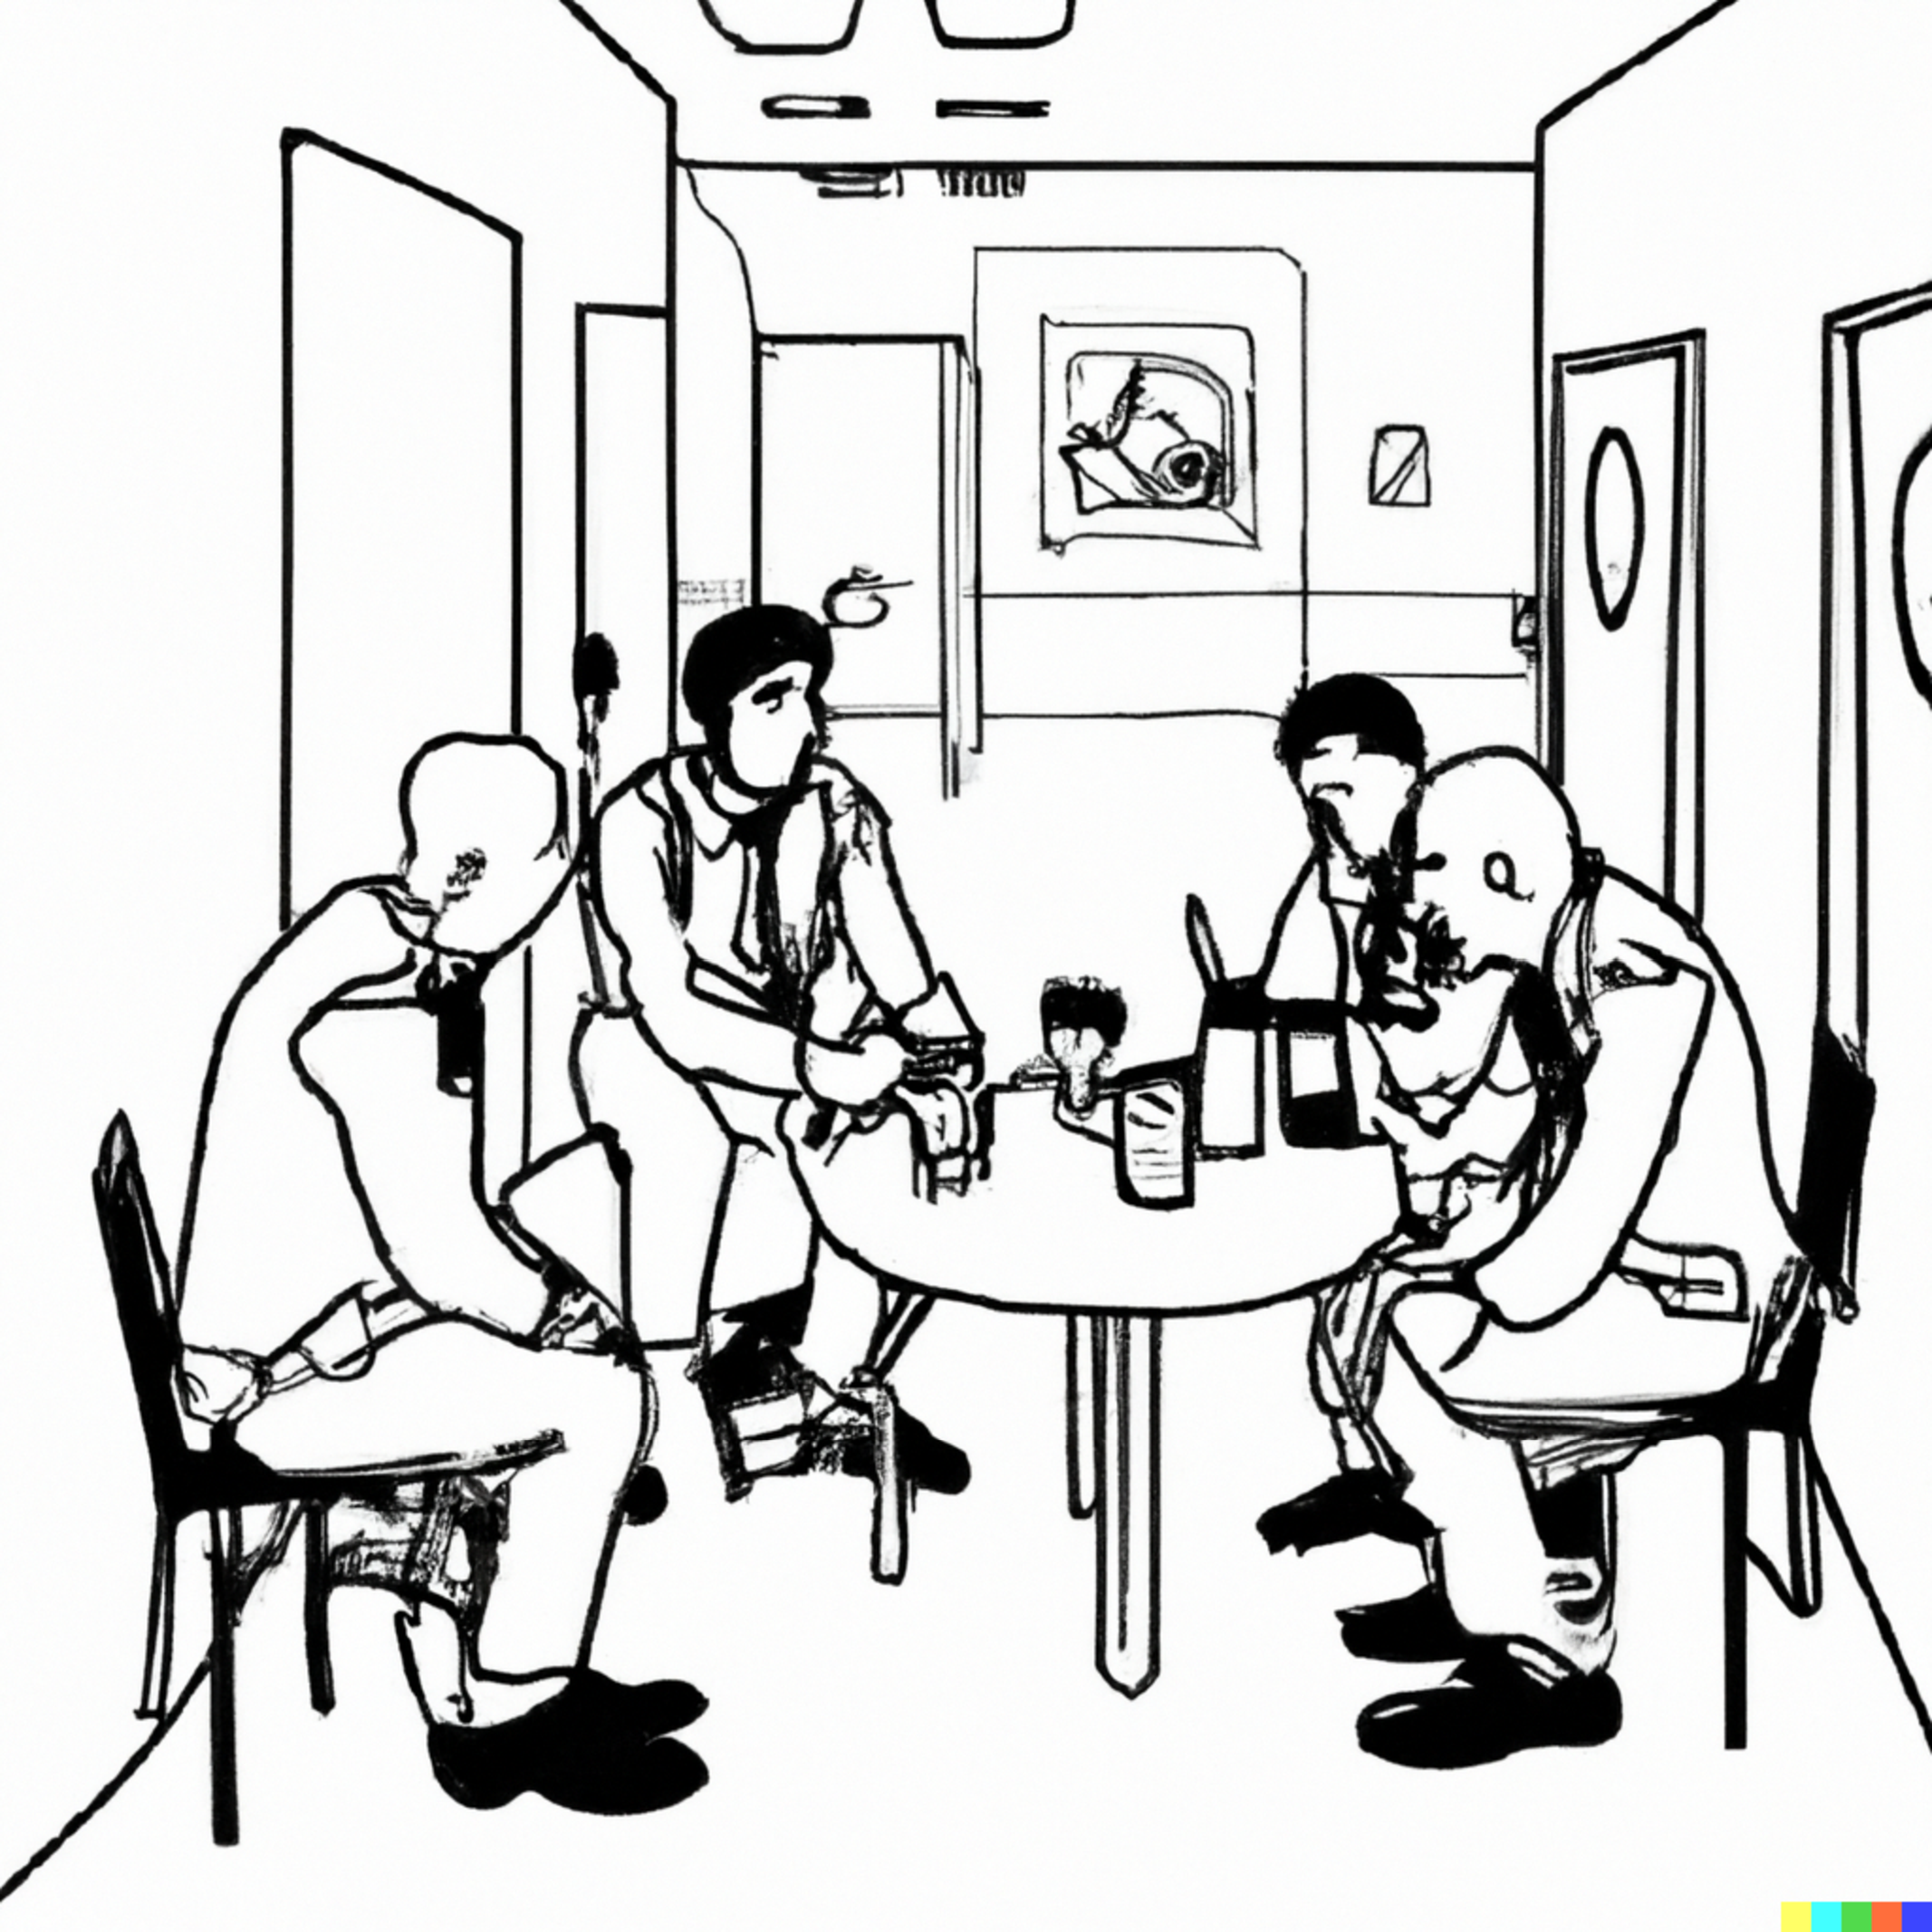
\includegraphics[width=0.8\textwidth]{images/bureaucrat_empathizing_with_coworkers_in_office_breakroom.pdf}
}

% This isn't monograph 
% "the readership has not only specialized or sophisticated knowledge but also professional interest in the subject of the work."
% -- https://en.wikipedia.org/wiki/Monograph
% Might be a https://en.wikipedia.org/wiki/Treatise

%\begin{figure}[H]
%    \centering

%    \label{fig:empathizing-in-breakroom}
%\end{figure}

% alternative titles:

% * How to Be an Effective Bureaucrat: A Field Manual

% * "You are a bureaucrat" -- probabilistically true, but not always
% * "How to Be an Effective Bureaucrat: A Field Guide" -- field guides are for wildlife spotting.  
% * "Everyone is a bureaucrat" -- false
% * "organization membership" -- bland
% * "administrivia"
% * "distributed knowledge and distributed decision-making"
% * "Distributed Decision-making"
% * "Be an Effective Bureaucrat: A Field Guide"
% * "How to be an Effective Bureaucrat: A Field Guide"
% * "Field Guide for Being An Effective Bureaucrat"
% * ""

\author{\huge Ben Payne}
\date{\today}

\begin{document}
\pagenumbering{alph} % Fixes problem with glossary links; see https://tex.stackexchange.com/questions/119527/glossary-backlink-points-to-wrong-page

% https://texblog.org/2012/02/08/adding-line-numbers-to-documents/
%\linenumbers


%\setcounter{secnumdepth}{1}
% -2 results in no numbering for chapters, sections, or subsections
% 0  results in no numbering for sections or subsections
% 1  results in no numbering for subsections


\begin{titlepage}
\maketitle
\thispagestyle{empty}
\end{titlepage}
\clearpage

\frontmatter % the front of the book has roman numerals

%\pagenumbering{gobble}
\thispagestyle{empty}

\noindent The Field Guide to Process Empathy. First Edition. Copyright \copyright 2022 by Ben Payne. 
% https://www.copyright.gov/help/faq/
Published under the 
\href{https://creativecommons.org/licenses/by-nc/4.0/}{Creative Commons Attribution-NonCommercial 4.0 International License}.


% https://tex.stackexchange.com/a/300368/235813
\vspace*{\fill}


% https://www.kith.org/words/2020/11/26/cataloging-in-publication-data/

\noindent Library of Congress Cataloging-in-Publication Data

\noindent Payne, Ben\\
The Field Guide to Process Empathy : How to be a Better Bureaucrat / Ben Payne. 1st ed.\\
% The “p. cm.” line is the “Physical description of the book, almost always blank since the books are usually not yet published” at the time when the CIP data is put together. Specifically, it's an indication of the page count and the book's size (in centimeters)
p. cm.

\noindent ISBN 979-8-9875369-0-2
\clearpage
\thispagestyle{empty}

\begin{center}
\noindent Thank you to my coworkers. \\Our interactions taught me \\how to be a better bureaucrat.
\end{center}%\clearpage
%\pagenumbering{roman}

\dominitoc % Initialization
\hypertarget{contents}{}
% https://tex.stackexchange.com/questions/553758/different-mechanics-of-hyperlink-vs-hyperref
\tableofcontents\label{sec:toc}

% 2022-07-11: Brian
%\chapter*{Preface}% * excludes from Contents
\chapter{Preface}


Bureaucracy is a consistent and pervasive challenge in modern society. You have direct experience with bureaucracy and are familiar with complaints about bureaucracy. You probably don't consider yourself a bureaucrat.

This book is intended to alter your view of bureaucracy. This book starts with an unconventional definition and then uses the definition to explain the necessity of various aspects of bureaucracy. Having identified specific challenges, the book serves as a guide for how you can be effective. 

A guide for situations you haven't been in before can decrease your anxiety by making the unfamiliar less intimidating. 
A guide labels patterns and provides context for your observations. 
Recognizing a familiar challenge can be preferable to the uncertainty of facing a novel scenario. An unfamiliar situation means not knowing how to start and not knowing the potential paths to success. In contrast, a challenge you understand can feel less burdensome. 
% 2023-01-05: Alicia@Upwork added the following sentence
Even if you have not faced the particular challenge before, a guide can make that new challenge seem familiar and manageable. 
Having a guide doesn't make your life easy -- even a challenge that is understood requires creativity and effort.

%If you don't think of yourself as a bureaucrat, I hope to change your mind on this essential topic. 

Having a guide isn't helpful if you find the topic repulsive.
Negative impressions of bureaucracy are common. The word
%bureaucracy 
% 2022-07-09: Jonah@upwork advocates removing this use
evokes reactions of disgust, primarily driven by how individuals have experienced bureaucracy.
The results of bureaucracy can appear idiotic -- 
% 2023-01-05: Alicia@Upwork says be more specific
wasting time and resources or causing harm to people.
%\footnote{In some dialects of Romani language, the word bureaucracy translates as ``the violence of paper.''}
%TODO: citation needed for Romani translation claim
% https://github.com/processempathy/bureaucracy-guidebook/issues/24
Bureaucracy is even regarded as dangerous to society.\footnote{``The only thing that saves us from the bureaucracy is inefficiency. An efficient bureaucracy is the greatest threat to liberty." (Eugene McCarthy, 1979~\cite{1979_McCarthy})}
% Time magazine, Feb. 1979
% https://en.wikiquote.org/wiki/Eugene_McCarthy
% https://time.com/vault/issue/1979-02-12/page/83/
I have bad news for you if you have a negative impression of bureaucracy: bureaucracy is vital to society. 

Having a precise definition of bureaucracy enables a more nuanced discussion.\nolinebreak 
\begin{quote}
\textbf{Definition}: 
\iftoggle{glossarysubstitutionworks}{\Gls{bureaucracy}}{Bureaucracy}
is the process of enacting policies through subjective decisions made by a person, typically in the context of managing access to a shared resource. Three roles are present: policy maker, bureaucrat, and subject.
\end{quote}

% Effective bureaucracy is  to modern society.
%Organizations have an insatiable need for members to perform a variety of tasks.

The concepts and techniques in this book are derived from this definition. For example, in an organization comprised of bureaucrats no one member knows everything and no one person decides everything, so bureaucracy relies on distributed knowledge and distributed decision-making amongst people with distinct roles.
%The resources managed by an organization can be either tangible or intangible. 
For more exploration of this definition, see the section ``\hyperref[sec:define-bureaucracy]{What is Bureaucracy?}''%
\iftoggle{haspagenumbers}{ on page~\pageref{sec:define-bureaucracy}.}{}


You can learn to skillfully navigate bureaucracy by using the techniques in this book. A skilled bureaucrat is more effective. That improvement enhances the organization you are a member of. Modern society is an interwoven fabric of organizations, with  bureaucracy being the crucial material.
Rather than ponder societal-scale concerns, this book focuses on the complicated and typical experience of a bureaucrat. 

The framing of how you think about bureaucracy shapes what action you feel is relevant for changing your environment. 
Suppose your assumptions are wrong about how the system of bureaucracy works. Then you will be trying to change the system to meet your incorrect expectations and your actions are likely to be wasted effort tackling irrelevant aspects. 
An accurate understanding of bureaucracy allows you to be more effective and your changes to the system are more likely to succeed. 


As an example of how the above definition is distinct from conventional definitions,%
\footnote{\href{https://www.merriam-webster.com/dictionary/bureaucracy}{Merriam-Webster's definition} focuses on government; the \href{https://en.wikipedia.org/wiki/Bureaucracy}{Wikipedia entry}
\index{Wikipedia!bureaucracy@\string\href{https://en.wikipedia.org/wiki/Bureaucracy}{bureaucracy}}
acknowledges non-governmental bureaucracy.} I view government as an instance of where bureaucracy occurs -- rather than equating government to bureaucracy. By the definition in this book, bureaucracy is not limited to governments. I use ``organization'' to encompass governments, corporations, non-profits, or any collection of people working together. As a consequence, many people are bureaucrats. 


The widely-held negative connotation of bureaucracy may lead you to reject the label of bureaucrat. Your recognition of your status as a bureaucrat matters even if you intentionally reject the label or do not recognize that you are a bureaucrat. How you behave and what you think your responsibilities are depend on how you label yourself.
% If you do not recognize that you are bureaucrat, you're less likely to be successful interacting with those around you. 
If you don't think of yourself as a bureaucrat, then you won't be able to distinguish what is your fault, what is the fault of your coworkers, what is the fault of management, and what is intrinsic to bureaucracy. 

Reasoning about bureaucracy is an accessible topic for every reader because we each have personal experiences.
A commonly held view is that the bureaucracies we work within are broken: participants are harmed and there is inequality. 
A counterargument is that the bureaucratic behavior observed is how the system was designed to work. There is a third argument: bureaucratic systems work in a degraded mode -- they are less efficient than what is possible. 
In this book I set aside the macro-scale questions of bureaucracy like the three arguments above and focus on the human-scale interactions that give rise to bureaucracy. Rather than complain about systemic problems, this book provides you with practical actions for situations you encounter.

Even people who are smart (e.g., they know history, they have memorized state capitals, they can do math) can struggle when faced with complex, large-scale distributed systems comprised of humans. Thinking about complex, large-scale systems is not part of the conventional education curriculum. This book will help you learn about bureaucracy, increase your ability to identify patterns, and apply relevant techniques. The pervasiveness of bureaucracy means the opportunities to apply the skills you learn in this book are many -- at your job, at the grocery store, in negotiations with your family.


The difficulties of bureaucracy are central to large societies that have complicated dependencies on the interactions of many people. From foundational services like the delivery of water and removal of sewage, to advanced manufacturing that relies on long supply chains, bureaucracy is essential.  The challenge of bureaucracy affects governments and companies in different societies of all scales. And bureaucracy is durable -- it has existed for thousands of years. Because bureaucracy is pervasive, tackling the topic of bureaucracy is exciting and crucial. The excitement comes from the opportunities available for the many potential improvements.
%I enjoy pondering hard problems and then leveraging insights gained from reflection.
Being an effective bureaucrat is important because bureaucracy can be a \href{https://en.wikipedia.org/wiki/Force_multiplication}{force multiplier}\iftoggle{WPinmargin}{\marginpar{$>$Wikipedia: Force multiplication}}{}
\index{Wikipedia!force multiplication@\href{https://en.wikipedia.org/wiki/Force_multiplication}{force multiplication}}
beyond what one person could achieve on their own.

% there's no avoiding the issue
Everyone is a bureaucrat because there are few alternatives to bureaucracy for a society constrained by finite resources. Gaining skills in navigating bureaucracy is helpful both for your happiness and the improved functioning of society. That may seem abstract and lofty, but the situation is inescapable: you are a member of society and benefit from participating in society. 


% Who this book is for

% from https://graphthinking.blogspot.com/2021/07/bureaucracy-book-outline.html
This book is for you if you are curious about the complex world we live in,  if you are thinking about how to contribute to society,  if you want your employment to have impact, or if your job is different from what you expected. This book will help you understand why and how innovation is suffocated within bureaucratic organizations. Understanding the challenges means you can design ideas that are more likely to succeed.


% What you should expect reading this book: 
Every person in society is a participant in bureaucracy. The purpose of this book is to decrease the surprise of that experience and better prepare you emotionally and intellectually for the toil of being a bureaucrat. You can improve your skills as a bureaucrat with focused reflection and a good guide like this book. 

The topic of bureaucracy spans academic disciplines - \href{https://en.wikipedia.org/wiki/Psychology}{psychology},
\index{Wikipedia!psychology@\href{https://en.wikipedia.org/wiki/Psychology}{psychology}}\iftoggle{WPinmargin}{\marginpar{$>$Wikipedia: psychology}}{}
\href{https://en.wikipedia.org/wiki/Sociology}{sociology},
\index{Wikipedia!sociology@\href{https://en.wikipedia.org/wiki/Sociology}{sociology}}
\href{https://en.wikipedia.org/wiki/Organizational_behavior}{organizational dynamics},
\index{Wikipedia!organizational behavior@\href{https://en.wikipedia.org/wiki/Organizational_behavior}{organizational behavior}}
\href{https://en.wikipedia.org/wiki/Public_administration}{public administration}, 
\index{Wikipedia!public administration@\href{https://en.wikipedia.org/wiki/Public_administration}{public administration}}
\href{https://en.wikipedia.org/wiki/Anthropology}{anthropology},
\index{Wikipedia!anthropology@\href{https://en.wikipedia.org/wiki/Anthropology}{anthropology}}
and  
\href{https://en.wikipedia.org/wiki/Political_science}{political science}. 
\index{Wikipedia!political science@\href{https://en.wikipedia.org/wiki/Political_science}{political science}}
Most bureaucrats have no formal training in any of these domains. This book is not written from an academic perspective; it is written by a practicing bureaucrat to serve as a guide to be read by bureaucrats. 


% What is the benefit of reading this book?
As a result of reading this book, you will be better able to recognize and navigate complex human interactions within your career and outside of work. Perspectives offered in this book can benefit you directly, whether by promotion in rank or title, increase in pay, successful completion of a project, or through decreased stress derived from an improved understanding of  bureaucracy. Being a more effective bureaucrat can also positively affect the causes you care about and the people you engage with.
% Affect is a verb. "to affect" meaning to influence or have an impact on something. Effect is the noun: "an effect" (a positive or a negative effect) is the result of being affected by something.


\subsection*{What this Book is Not}

This book is not a defense of bureaucracy, nor is it intended to disparage bureaucrats or the system of bureaucracy. Instead, this book is a guide to bureaucracy-as-it-is. There are no hacks presented for circumventing bureaucracy. Instead, this book provides advice on being an effective member of a bureaucratic organization.

This book does not focus on leadership, managing a team, being a team member, planning, time management, project management, advancing your career, promotions, or self-improvement. In the process of being a better bureaucrat, some lessons may apply in those domains.


Nothing in this book is domain-specific, nothing is tied to the engineering of products, and nothing applies solely to science research or policy development. However, skills associated with being an effective bureaucrat do translate into other domains.


This book does not discuss work conditions, pay, benefits, or retirement plans. If you are seeking a competitive advantage that might result in improved outcomes, learning to navigate bureaucracy helps.


This book doesn't focus on citizens, political 
\iftoggle{glossarysubstitutionworks}{\glspl{policymaker}}{policymakers}, oversight (e.g., Congress at the state or federal level, Inspectors General), 
competing organizations, contracts, the budget of an organization, fines and other regulatory punishments resulting from bureaucracy, policy enforcement, specific policies and regulations, formal arbitration or judicial resolution of disputes. For observations on those topics, see Wilson's \textit{Bureaucracy}~\cite{1991_Wilson}. 


This book doesn't discuss discrimination or harassment. I neglect differences in experience based on race, gender, or socioeconomic status. This book doesn't discuss bad coworkers, abusive bosses, psychological defects of individuals, or malicious intent. I assume no traitors, spies, \iftoggle{WPinmargin}{\marginpar{$>$Wikipedia: saboteurs}}{}
or saboteurs~\cite{1944_War_Dept}. I do not discuss \href{https://en.wikipedia.org/wiki/Dark_pattern}{dark patterns}; 
\index{Wikipedia!dark pattern@\href{https://en.wikipedia.org/wiki/Dark_pattern}{dark pattern}}
issues like lying, bribery~\cite{2021_Ang}, and criminal behavior are not discussed. Those aspects happen whenever people interact, so  the challenges of intentional defectors are not specific to bureaucracy. 

Bureaucracy is not a manifestation of incompetence, laziness, or mistakes.
% removed "malicious actors" from list
% malice
Even with well-trained bureaucrats trying to help other people, challenges arise when people interact to manage access to a shared resource. 
%The Good Samaritan is more applicable than a rational actor model
Sources of friction in a well-run bureaucracy stem from  ambiguity, conflicting incentives, finite attention, and inadequate resources. Bureaucracy is only necessary because shared resources are scarce. There's not enough to satisfy the needs of the community, leading to contention. Therefore distributed decision-making and distributed knowledge are relevant for the allocation of those resources.


Focusing on the morals of organizations or bureaucrats~\cite{2009_Jackall} is less compelling than studying bureaucracy because norms (i.e., expectations for individuals and organizations) shift over time, while bureaucracy is persistent. 
In this book I focus on culturally invariant aspects of bureaucracy. 


\subsection*{Assumptions}
As a way of limiting the complexity of this book, I assume you are honest and that other people are honest. 
%That isn't always applicable, but I'm aiming to describe __(?)
I assume bureaucrats strive for fairness, though the definition of fairness may vary from bureaucrat to bureaucrat. 
The complexities of bureaucracy arise even with these simplifying assumptions.% and unaddressed topics. 
My guidance on how to be an effective bureaucrat applies to  bureaucracy that was intended to be helpful (rather than malicious).



% Source of this content: 
This book is based on personal experience operating in multiple large organizations and small teams, reading published books and papers, and insight from fellow bureaucrats. Informal surveys were conducted but are not foundational for claims made in this book.%
\iftoggle{WPinmargin}{\marginpar{$>$Wikipedia: blinded-experiment}}{}
No \href{https://en.wikipedia.org/wiki/Blinded_experiment}{double-blind}%
\index{Wikipedia!blinded experiment@\href{https://en.wikipedia.org/wiki/Blinded_experiment}{blinded experiment}}
experiments were conducted. 
% my experience
% I wrote this book for a younger version of me.
% When I first started my job in a large organization I recognized differences between the expectations of the education system I had left and the challenges of a professional environment. 
I have tried to learn from my mistakes by reflecting on my (in)actions and the consequences. This haphazard approach has been an expensive education. My mistakes delayed progress and damaged relationships. This book  provides generalizations from my experiences that might benefit the reader. My hope for this guide is to decrease your surprise when you encounter what would have been novel situations.

\ \\

% How the book should be read: 
Reading this book front-to-back is the default option, but not required. The dependencies of topics are not sequential -- see Figure~\ref{fig:core-concepts}.

\begin{figure}[ht]
    \centering
    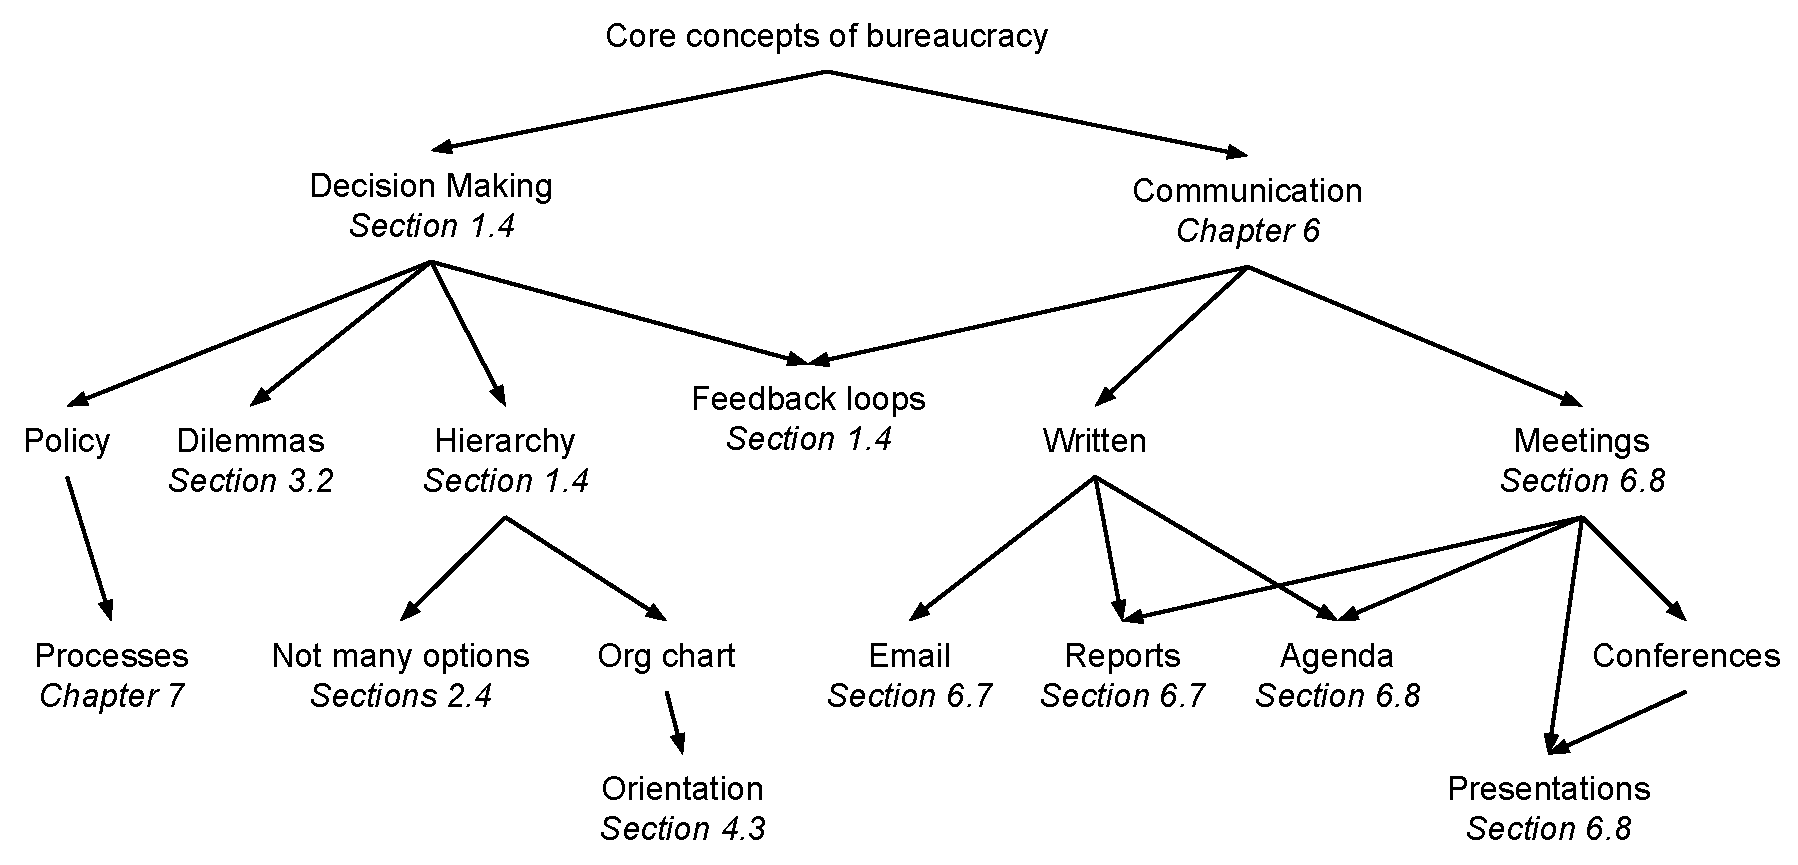
\includegraphics[width=1\textwidth]{images/core_concepts_map.pdf}
    \caption{Relation of the concepts related to bureaucracy discussed in this book.}
    % TODO (aspirational): generate diagram from Latex
    \label{fig:core-concepts}
\end{figure}

% 2022-03-27: BHP was not impressed by the options on https://texample.net//tikz/examples/tag/graphs/ including the "mindmap" option
% this looks better: http://randomresearchdata.blogspot.com/2013/12/tikz-simple-decision-tree-or-cart-tree.html
% see https://texample.net/tikz/examples/feature/trees/

%\begin{tikzpicture}[main/.style = {draw, circle}] 
%\node[main] (1) {Core Concepts}; 
%\node[main] (2) [above right of=1] {Decision-making}; 
%\draw[->] (1) -- (2);
%\end{tikzpicture} 

The approach in this book is to view bureaucracy from a few perspectives. The first is a conceptual view focused on the \hyperref[sec:define-bureaucracy]{definition of bureaucracy} %\iftoggle{haspagenumbers}{ (page~\pageref{sec:define-bureaucracy})}{}
in terms of managing shared resources. The second view is structural (e.g., hierarchy, meetings). The \hyperref[sec:fundamentals-of-b]{essentials of bureaucracy}%
\iftoggle{haspagenumbers}{ (page~\pageref{sec:fundamentals-of-b})}{} 
will be familiar to experienced bureaucrats. 
The third view is based on the experience of a practicing bureaucrat -- 
\hyperref[sec:dilemma-trilemma]{dilemmas}\iftoggle{haspagenumbers}{~(page~\pageref{sec:dilemma-trilemma}),}{,}
\hyperref[sec:unavoidable-hazards]{unavoidable hazards}\iftoggle{haspagenumbers}{~(page~\pageref{sec:unavoidable-hazards}),}{,}
and 
\hyperref[sec:effective-bureaucrat]{tips on how to be effective}\iftoggle{haspagenumbers}{~(page~\pageref{sec:effective-bureaucrat}).}{.}

%The three productive views of bureaucracy (concept, structure, experience) are contrasted with~\hyperref[sec:alternative-views-from-within]{how other bureaucrats view bureaucracy} and~\hyperref[sec:models-of-bureaucracy]{other models of bureaucracy}.

Chapters~\ref{sec:introduction} %\iftoggle{haspagenumbers}{(page~\pageref{sec:introduction}) }{}
through~\ref{sec:why-bur-hard} %\iftoggle{haspagenumbers}{(page~\pageref{sec:why-bur-hard}) }{}
provide background context for bureaucracy. 
Chapters~\ref{sec:individual-in-org} %\iftoggle{haspagenumbers}{(page~\pageref{sec:individual-in-org}) }{}
through~\ref{sec:process} %\iftoggle{haspagenumbers}{(page~\pageref{sec:process}) }{}
are the guide. 
You can read each chapter of the guide independently. 

The freely available electronic versions of this book (including 
\index{Wikipedia!PDF@\href{https://en.wikipedia.org/wiki/PDF}{PDF}}\iftoggle{WPinmargin}{\marginpar{$>$Wikipedia: PDF}}{}
\href{https://en.wikipedia.org/wiki/PDF}{PDF}, 
\index{Wikipedia!HTML@\href{https://en.wikipedia.org/wiki/HTML}{HTML}}
\href{https://en.wikipedia.org/wiki/HTML}{HTML}, and 
\index{Wikipedia!EPUB@\href{https://en.wikipedia.org/wiki/EPUB}{EPUB}}
\href{https://en.wikipedia.org/wiki/EPUB}{EPUB} 
formats) have hyperlinks in the text. Light-blue hyperlinks reference external resources like Wikipedia, while dark-blue links reference material within the guide such as the glossary. 
%The PDF and printed versions have notes in the margin to help identify the links.


\ \\

% as per https://tex.stackexchange.com/q/393238/235813
\begin{flushright}
Ben Payne\\
\today\\
United States of America\\
Earth
\end{flushright}


%\clearpage
%\thispagestyle{empty}

\mainmatter % the main part of the book will have standard pages

% https://tex.stackexchange.com/questions/2958/why-is-newpage-ignored-sometimes


% https://tex.stackexchange.com/questions/5894/latex-conditional-expression
\newif\ifpageref
\newif\ifsectionref
\pagereffalse
\sectionreffalse

% etoolbox
\newtoggle{pageref}
\newtoggle{sectionref}

\togglefalse{pageref}
\togglefalse{sectionref}



\chapter{Introduction\label{sec:introduction}}
{\footnotesize Back to the \hyperref[sec:toc]{Main Table of Contents}}
\minitoc
%  Section~\ref{sec:define-bureaucracy} defines bureaucracy and associated terminology for specific roles. That is contrasted in section~\ref{sec:alternative-views-from-within} with how bureaucrats view themselves and their interactions. In section~\ref{sec:models-of-bureaucracy} a summary of external perspectives of bureaucracy is provided. 
  
  The motivating logic for this book is a sequence of claims:
\begin{enumerate}
    \item A community has limited resources that members desire. The members of the community respond to that constraint by sharing resources.
    \item Contention amongst community members regarding access to a \gls{shared resource} leads to a need to manage access.  
    \iftoggle{glossaryinmargin}{\marginpar{[Glossary]}}{}%
    Managing access requires making and enforcing policies that apply to community members. This may start as a consensus but often a single person is nominated because the cost of consensus is high. This is not yet bureaucracy because subjects can negotiate with the person managing access to the resource.
    \item Due to increased size or complexity, more than one person may be responsible for making and enforcing policies. Having multiple policymakers leads to inconsistent policies, so instead the workload is split into the roles of policymaker and policy execution by a bureaucrat. 
    \item 
\iftoggle{glossarysubstitutionworks}{\Gls{bureaucracy}}{Bureaucracy}
exists when people involved in managing access to 
\iftoggle{glossarysubstitutionworks}{\glspl{shared resource}}{shared resources} have the roles of policymaker, bureaucrat, and subject.
%While bureaucracy arises in response to  bureaucracy can exist without being assocaited with a shared resource.
    \item Managing access to shared resources can involve multiple bureaucrats operating together. In a large organization the use of distributed knowledge and distributed decision-making results in \gls{decentralized bureaucracy}.
    \item Whether you're a \gls{bureaucrat} 
    \iftoggle{glossaryinmargin}{\marginpar{[Glossary]}}{}%
    or a subject of bureaucracy, you can be more effective by applying \hyperref[sec:process-empathy]{process empathy}.
    %\marginpar{See page~\pageref{sec:process-empathy}.}
\end{enumerate}

Once you've familiarized yourself with the concepts in this book, using what you've learned is a two-step process. First, ask yourself whether the conditions for bureaucracy are present. If they are, then you can be more effective by applying process empathy.

The definition of bureaucracy is the basis for evaluating the scenario you are in. You may already have a sense of what bureaucracy is, but a description is provided
\iftoggle{haspagenumbers}{ on page~\pageref{sec:define-bureaucracy}}{} 
in the section~\hyperref[sec:define-bureaucracy]{``What is Bureaucracy?''} To supplement the definition, illustrations of bureaucracy provided throughout this book show how you can grow your process empathy -- the focus of the next section.  \clearpage
  \section{Process Empathy\label{sec:process-empathy}}

Empathy typically refers to understanding the emotions of another person. To detect the emotional state of another person you rely on facial expressions (smiles for happiness, frowns for frustration), body language (arms crossed, turning away), speech (yelling in anger, singing for joy), and actions (hitting something). From these signals you evaluate a person's emotional state by recalling instances where you felt similar emotions. Emotional empathy helps you understand another person. 

A distinct form of empathy is the ability to understand the reasoning another person uses.  
\hyperref[sec:intellectual-empathy]{Intellectual empathy} is helpful for enabling a common understanding of an issue. That applies both one-on-one and with a team of people. Intellectual empathy is enacted by thinking about how another person would assess a situation and they might respond. Another technique is to imagine what reasoning they would use when presented with a set of facts. 


A third form of empathy is the focus of this book: the ability to perceive why individuals working together behave in recurring patterns. What incentives do people in each role have, what information does each person have, and how does that manifest as actions by the team or organization? Applying the paradigm of \gls{process empathy} helps you answer questions like ``Why is this taking so long?'' and ``Why is this action so apparently inefficient?'' The answers come from recognizing \hyperref[sec:unavoidable-hazards]{unavoidable hazards} of bureaucracy. As another example, the question ``Why are people under-trained for their role?'' is answered by constant \hyperref[sec:turnover]{turnover}. Process empathy relies on understanding bureaucracy so that you can distinguish which patterns are specific to the people involved versus specific to this organization versus generic to every organization.

Reasoning about a process is slightly different from process empathy. Reasoning assumes a holistic external view (taken by Gall in~\cite{2002_Gall}), whereas process empathy is about the perspective of individual people operating within their local context. Reasoning about teams and the aggregate organization invariably leads to observations of illogical and absurd outcomes, whereas a view based on process empathy reveals the causes of apparent paradoxes.

Process empathy is comprised of thinking beyond professional relationships with individuals and deeper than the abstraction of team-as-entity and organization-as-entity. 
Because process empathy is generic across bureaucracies, the benefit of this perspective is that you can gain insight about people you don't know doing work you don't understand.
Each application will have nuances specific to the people involved and the shared resource being managed, but process empathy provides a useful framework for navigating bureaucracy.


Process empathy involves asking questions about your situation:
\begin{itemize}
    \item What incentives do process participants face?
Also consider the (lack of) \hyperref[sec:feedback-loop-and-ripples]{feedback loops} (page~\pageref{sec:feedback-loop-and-ripples}).
    \item What unaligned goals do individual bureaucrats have that cause friction?
    \item What are the different paths individual bureaucrats take to work towards their goals?
See \hyperref[sec:dilemma-trilemma]{dilemmas} on page~\pageref{sec:dilemma-trilemma}.
    \item How to leverage the interplay between processes and interpersonal professional relationships?
See \hyperref[sec:reputation]{reputation} management on page~\pageref{sec:reputation}.
\end{itemize}

Rather than asking about ``what benefits the team?'' or ``what supports the organization?'' the paradigm of process empathy focuses on people and incentives. For you this translates to specific actions. For example, to be effective you need to 
identify rules (written and unwritten), determine who enforces what, consider the detection mechanics, and weigh the consequences of subversion against the benefits of breaking rules.


The question of ``when is process empathy applicable?" is answered by ``when bureaucracy is present?" which requires a definition of bureaucracy. 
 \clearpage
  \section{What is Bureaucracy?\label{sec:define-bureaucracy}}

While you may know it when you see or experience bureaucracy, for this book definitions are useful. Throughout the book we'll refer back to these definitions as we build out the concepts needed to understand bureaucracy.

\index{bureaucracy!definition of}
\Gls{bureaucracy} involves creation and execution of \glspl{policy} for managing shared resources. Creating and carrying out policies usually involves multiple people, with each person having specialized roles. Task scalability (how many widgets), complexity (number of tasks per widget), or latency (time per widget) motivate members with distinct roles to form a hierarchical organization to facilitate coordination. The organization has control over the disbursement of resources relevant to the society the organization operates within, or the organization administers a policy within that society. Resources managed by the organization are either tangible (e.g., water, air, land) or expertise.  

Bureaucracy is not limited to government. Non-profit organizations, volunteer groups, commercial companies, and even small teams of people can invoke bureaucratic tendencies. The existence of bureaucracy is independent of an organization's purpose, and independent of whether money is involved. Carrying out someone else's subjectively defined policy will require you to make your own subjective decisions regarding execution and enforcement. 

\ \\

With bureaucracy defined, distinct roles can be identified.
\index{bureaucracy!roles}
A bureaucracy typically involves a policy creator, a policy enforcer, and the person upon whom policy is inflicted. In the context of government, the policy creator can be either a politician or a bureaucrat. 

An organization comprised of bureaucrats is a \gls{bureaucracy}. The main character within a bureaucracy is the \gls{bureaucrat} -- the person who is a member of an organization and is responsible for subjective implementation of policy for the organization. The person that a bureaucrat's decisions are inflicted on a \gls{subject}.  Depending on context, a subject may be a student (when the bureaucrat is a teacher) or a subject may be a citizen if the bureaucrat is a police officer or government official. Sometimes a bureaucrat's decisions are inflicted on other bureaucrats-as-subjects, such as when a Chief of Police creates guidelines for police in their district, or when a senior diplomat sets policy for embassy employees. 


A \gls{bureaucrat} is a person subjectively interpreting policies on behalf of an organization and has discretionary enforcement. The bureaucrat's purpose is to facilitate coordination of stakeholders by applying specialized knowledge. 

Let's break that down piece-by-piece. First, ``subjective interpretation'' means there is a person making a decision about how to do something. The subjectivity arises from different reasons one person might choose an option over a competing option.  A \gls{policy} is a set of actions in a given circumstance. An \gls{organization} is the collection of people for who the policy is made. Discretionary enforcement means the person is choosing how to apply the policy in the specific circumstances. Facilitating coordination means bureaucracy is about getting multiple people (or sometimes a person at different instances in time) to work together. The stakeholders are people who care about the application of the action in each circumstance.  That's still pretty dense, so the rest of the book is spent expanding the nuances and implications of this definition.

Bureaucracy is neither good nor bad. Bureaucracy is not tied to politics, nor is bureaucracy specific to an institution (corporations, governments, academia). The definition of bureaucracy used in this book is independent of government. Bureaucracy is not defined to be efficient; nor does it have to be inefficient. Bureaucracy is not restricted to paperwork, record keeping, quantification, or gathering metrics. Nothing in this definition involves paperwork or an office building. Definitions that limit the concept of bureaucracy to specific contexts result in a decreased ability to describe complex large-scale human organizations. 

Bureaucracy is about delegation of control, communication, decision making, coordination, and processes. Bureaucracy relies on negotiation. 

\begin{figure}
    \centering
    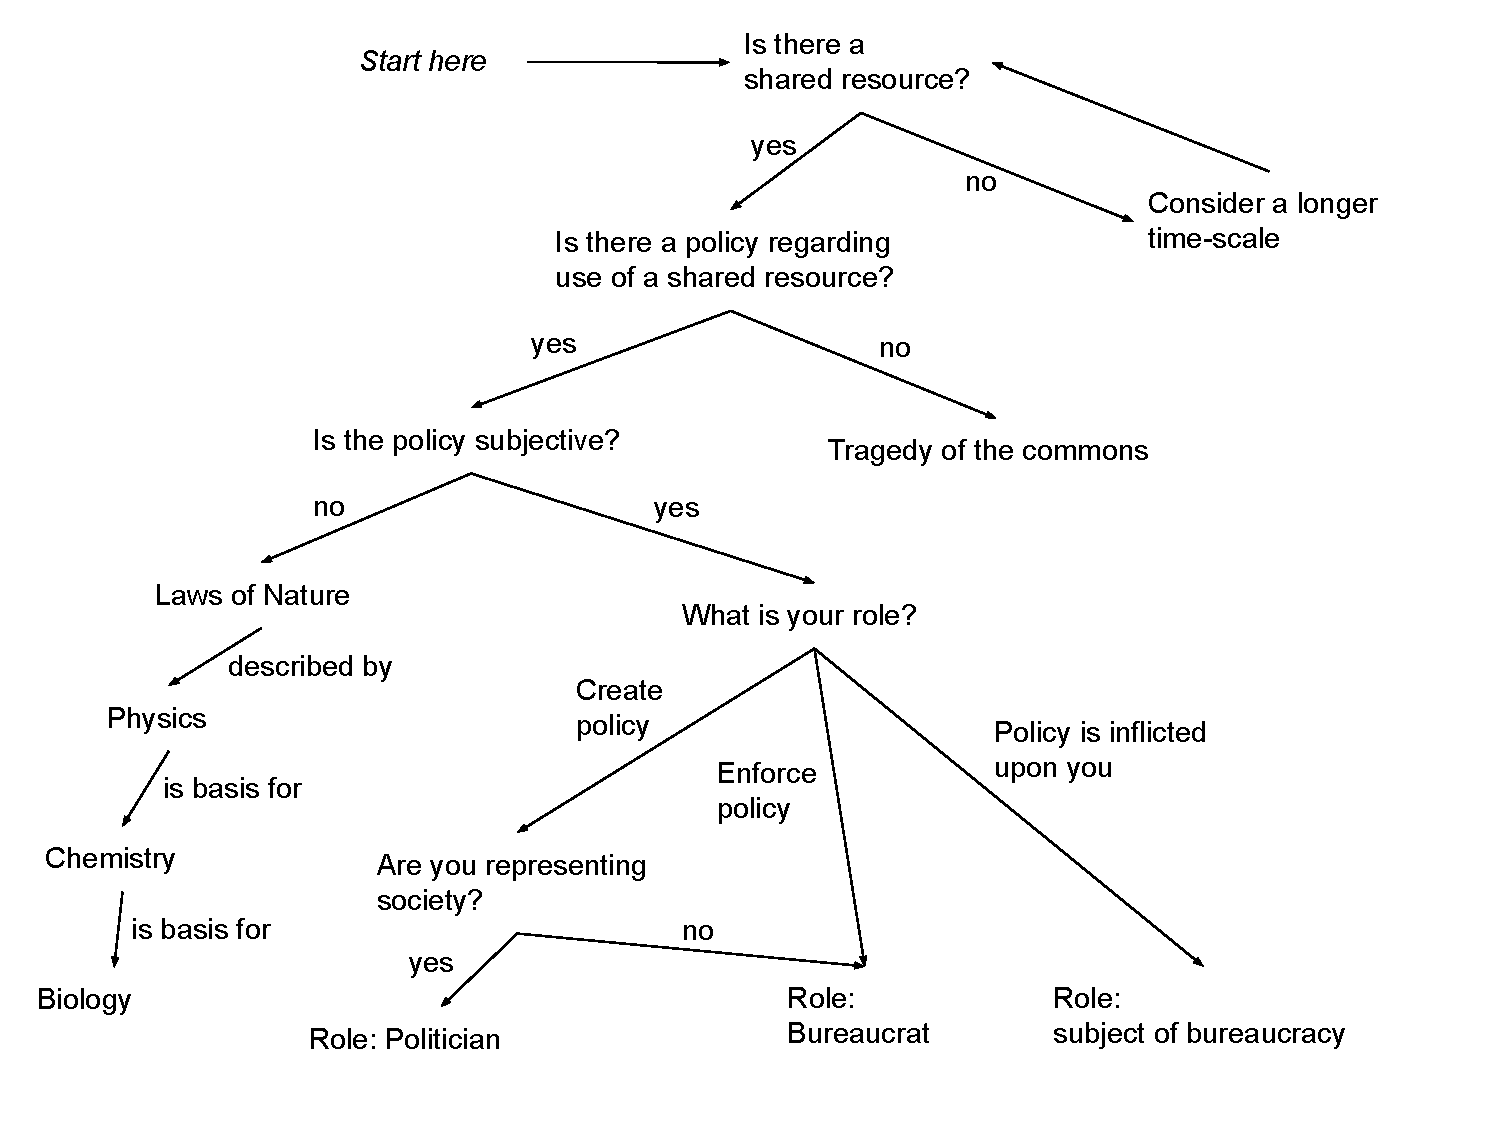
\includegraphics[width=1.05\textwidth]{images/am_I_a_bureaucrat.pdf}
    \caption{Decision tree for determining whether you qualify as a bureaucrat}
    \label{fig:am-I-a-bureaucrat}
\end{figure}

A critical aspect of bureaucracy is that everything is made up, specifically by other humans. The consequence is that everything is negotiable. You (in the role of either a subject or a bureaucrat) need to know both who to negotiate with and how to negotiate the desired changes. My claim that bureaucracy is made up is in contrast to actual rules -- the mathematical physics that describe nature. Everything in your environment is either naturally occurring macroscopic emergent phenomena (e.g., chemistry, biology) or humans making up labels and norms. Distinguishing the two is critical to knowing what you can change and what you have to operate within. 

Bureaucracy arises when there is no common, objectively quantifiable feedback mechanism for individual participants in the organization. This aspect is why governments, schools, and prisons are characterized as bureaucratic. The military doesn't rank soldiers by ``number of enemies killed'' and is bureaucratic. Even profit-driven commercial organizations are bureaucratic when the impacts of individual employees are not coupled to the metrics of profit. 

Profit-based feedback makes some roles in a business context slightly more predictable and understandable. Even in that situation there are trade-offs like externalization of costs and long-term profit versus short-term profit. 

The concept of bureaucracy is most visible for complex recurring situations involving many people and the control of a shared resource. The apparent friction of bureaucratic processes can be lower when there are only a few people involved (``I'm just talking to my collaborator" or ``I'm just buying groceries from a clerk at the store'' or ``I'm using a website for a government service''), but there is a continuous gradient to more obvious instances of bureaucracy. Bureaucratic tendencies are observable at the small scale; they typically get ignored or called something else.

Bureaucracy arises when management of a shared resource is necessary; that resource can be external to the organization or internal to the organization. Examples of external resources include mail delivery for \href{https://en.wikipedia.org/wiki/United_States_Postal_Service}{USPS}, public safety for \href{https://en.wikipedia.org/wiki/Federal_Bureau_of_Investigation}{FBI}, and the environment for \href{https://en.wikipedia.org/wiki/United_States_Environmental_Protection_Agency}{EPA}. The focus of this book is on internal resources. Resources internal to a bureaucratic organization include intangibles like attention, skill, expertise. Metrics like time, money, and staffing are proxy measures for the central intangible resources.



Bureaucracy is a system for distributed knowledge and distributed decision making. 
\index{bureaucracy!definition of}
That is in contrast to easier-to-understand concepts like centralized knowledge and centralized decision making. A government run by dictatorship is easy to conceptualize compared to democracies because there is a central character around which a narrative can be formed. Similarly, stories about the \href{https://en.wikipedia.org/wiki/Chief_executive_officer}{CEO} of a company are much easier than capturing the thousands of interactions conducted by the many employees of that company. The vast majority of the work an organization does is coordinated and carried out by people other than the CEO. Linear story-telling with a small number of main characters does not map well to the complexities of bureaucracy. 


  \clearpage
  \section{The Scope of Bureaucracy}
Bureaucracy is a trait of an organization: we call organizations bureaucratic. This is consistent with the definition of bureaucracy based on managing \glspl{shared resource}.  \iftoggle{glossaryinmargin}{\marginpar{[Glossary]}}{}
Examples of organizations considered bureaucratic include:
  \begin{itemize}
      \item The \href{https://www.epa.gov/}{Environmental Protection Agency} (EPA) manages access to bureaucrats who have expertise with environmental regulations governing water, air, workplace safety, etc.
      \index{exemplar!Environmental Protection Agency (EPA)}
      \item The \href{https://www.intelligence.gov/}{United States Intelligence Community} manages access to bureaucrats who have expertise in collecting foreign intelligence.
      \item The information technology department in a large organization manages staff with expertise in repairing computers.
      \index{exemplar!information technology department}
      %\item Human resources department
      \item Bureaucrats in the \href{https://www.fda.gov/}{Food and Drug Administration} (FDA) use their expertise to regulate food safety to serve their community.
      \index{exemplar!Food and Drug Administration (FDA)}
      \item Bureaucrats of the \href{https://www.faa.gov/}{Federal Aviation Administration} (FAA) have expertise on flight safety to protect their community.
      \index{exemplar!Federal Aviation Administration (FAA)}
      \item The military manages the shared resource of bureaucrats with expertise in war-making.
      \index{exemplar!military}
  \end{itemize}

These descriptions of bureaucracy are conceptually consistent but don't provide value to you, the practicing bureaucrat. Bureaucracy is not a distant, faceless concept. Bureaucracy permeates your environment and is the basis for many interactions you have with other people. 

When you recognize bureaucracy specific to your environment, you will be able to respond appropriately. If you recognize the systemic incentives driving a person's behavior, you are less likely to see the person as malicious or incompetent. You are also more likely to be able to negotiate with them and enact the changes that you seek.
    \subsection*{Who is a Bureaucrat?}

A cashier in a gas station is a bureaucrat. 
\index{exemplar!store clerk}
The shared resource is the gas and other items for sale. The ``policy'' might be ``take money from customer in exchange for items sold in the store and gas from the pumps,'' but the subjective application of that policy leaves a lot of room for the cashier to shape the customer's experience. Does the cashier greet the customer when the customer enters the store? Does the cashier look at the customer to acknowledge the customer? Smile? How quickly does the cashier engage the customer? Minor nuances left to the cashier in the execution of the store policy mean there is room for subjective application of the policy. 

% examples of bureaucrats
A bank teller, a loan officer, and a bank's \href{https://en.wikipedia.org/wiki/Technical_support}{technical support} 
\index{Wikipedia!\href{https://en.wikipedia.org/wiki/Technical_support}{technical support}}
\marginpar{[Wikipedia] Technical\\support}
are all bureaucrats. 
\index{exemplar!bank employees}
The shared resource includes money the bank manages and the expertise associated with managing money. Each employee subjectively enforces policies on behalf of the organization. Each role has a different amount of impact on the bank's finances. Of these three roles, the loan officer's interactions with bank customers provide the most straightforward route for feedback based on profit. The loan officer doesn't act alone though -- the customer's interactions with tellers and the bank's technical systems also matter to the customer's decision about how and where to manage money. 


This same discretionary application of policy applies to commercial bureaucrats like sandwich makers, car salespeople, oil well drillers, grocery clerks, retail clerks, 
\index{exemplar!store clerk}
and plumbers. Public school teachers, state and federal police, 
\index{exemplar!law enforcement officers (LEO)}
military members, 
\index{exemplar!military}
tax collectors, and other state workers are government bureaucrats. 


% bureaucracy is not limited to white collard office workers
Factory line workers subjectively apply policies, with the assembly line and factory being the shared resource. Enforcement of quality standards is a subjective policy. The pacing of work is a negotiation with management that directly impacts productivity and profits. The feedback loop for factory workers from profit generated by the product is weak and diffuse. %The shared resources governed by the worker's policies include the work environment, product quality, productivity, and profit.

Structured environments like sports featuring well-defined rules do not eliminate bureaucracy. Teammates use subjective policies on who to work with and how to best leverage their strengths and exploit the opponent's weaknesses. The policies are set in part by the coach. Referees make subjective determinations about rules.

Sometimes bureaucrats do not work directly with customers or citizens or products. Then the bureaucratic process is inflicted on fellow bureaucrats. In that scenario, a bureaucrat is subjectively applying a policy to other bureaucrats. 

\ \\


\begin{quizbox}{
      \textit{Self-administered exam}: 
      \textbf{Am I a Bureaucrat?}
}
Answer Yes or No for each of the following descriptions:
\begin{itemize}
    \item I rely on the knowledge of others. 
    \item The outcome of other people's decision-making informs my actions. 
    \item I administer subjectively determined policies for a shared resource. 
\end{itemize}
If all three of these are true for you in a specific context, then you are a bureaucrat. In situations where these conditions are not applicable, you are not a bureaucrat.
\label{box:self-administered-exam}
\end{quizbox} 
See Figure~\ref{fig:am-I-a-bureaucrat} \iftoggle{haspagenumbers}{ on page~\pageref{fig:am-I-a-bureaucrat}}{}
for a more detailed evaluation.

\ \\

Identifying yourself as a bureaucrat matters because the label informs the responsibilities of your role. The risk of not self-identifying as a bureaucrat is that you won't grasp how much control you have in enacting and enforcing policy. If you think of yourself as having to blindly follow rules, you will harm the people you are applying the rules to and the organization you are applying the rules for. The value of having capacity for judgment is so you can adapt policies to circumstances. Power is merely decisions that alter the opportunities of other people, so your self-perception of what decisions are available determine how much power you have.

In a similar sense from the consumer's or citizen's perspective, if you don't think you are interacting with a bureaucracy, you won't perceive the opportunity to negotiate.  If you view rules as unchanging and inflexible, you will harm your ability to make progress. If a human made a rule, then that rule is flexible. Who made the rule? Who enforces the rule? If you can talk to them, could they be convinced to make a modification or an exception? Sometimes the answer is yes.

If you don't think about the bureaucratic framing, you might think the store clerk is enforcing a policy because they don't like you. Assigning personality conflict as the cause might lead to a different conversation with their manager (the person who created the policy). 

If you don't think of yourself as a bureaucrat, you may behave passively in your job. The paradigm of ``just tell me what to do'' is the default (learned in school) and you won't know how to engage with coworkers and bosses since their role is distinct from that of a friend. You will be less likely to understand how to leverage members of your organization. Thinking from a bureaucrat's perspective explains why communicating within your organization is critical to your success and the organization's success. 
%You'll see your coworkers as competitors for promotion.

% https://graphthinking.blogspot.com/2020/10/impact-of-self-identifying-as-not.html
If you think of yourself as merely a cog in a machine, you are less likely to notice that you exert influence in the process and you are less likely to recognize the autonomy available to you. 
If you think ``I have a real job (e.g., nurse, cashier, teacher); therefore I'm not a bureaucrat", you are less likely to recognize the subjective power you have in interactions with the public.
If you think, ``I'm at the bottom of my organization's hierarchy; therefore I do not have power", you are less likely to notice autonomy when it is available.

If you don't consider yourself to be part of a bureaucratic process, you'll behave differently in interactions with bureaucrats.  You won't perceive opportunities to negotiate because the processes seem fixed instead of subjective. 
You won't recognize motives and incentives of bureaucrats, so their activities will seem incomprehensible. Once you identify as an important part of the bureaucratic process, you will be able to effectively engage, negotiate, and make meaningful changes happen.


  \clearpage% subsection
    \subsection*{Factors Influencing Bureaucracy}

Although bureaucracy can be present for one person, and bureaucracy is often apparent on teams (e.g., 3 to 20 people), this book focuses on the situation of multiple teams comprising an organization. The size of an organization might be a few hundred people (above \href{https://en.wikipedia.org/wiki/Dunbar's_number}{Dunbar's number}
\index{Wikipedia!\href{https://en.wikipedia.org/wiki/Dunbar's_number}{Dunbar's number}}
) up to millions of people. 
Examples of companies that employ more than a million people\footnote{See \href{https://en.wikipedia.org/wiki/List_of_largest_employers}{Wikipedia's list of largest employers}.
\index{Wikipedia!\href{https://en.wikipedia.org/wiki/List_of_largest_employers}{list of largest employers}}
} include Walmart, Amazon, and McDonald's. Size isn't a requirement for bureaucracy. Small companies with a few people incur bureaucracy because of the need to coordinate subjective policies governing shared resources. 

Money is uncorrelated with bureaucracy. Bureaucracy occurs in commercial companies, government, and non-profit organizations. Money can help align incentives and provide feedback loops to inform behavior, but it can also be the source of administrivia and policies. 

Bureaucracy emerges in small organizations, has scale-invariant patterns, and is generic across sectors. The complexity of the tasks may differ, but the same scale-independent patterns  emerge because of a common factor: human behavior.

% https://graphthinking.blogspot.com/2017/05/population-sizes-needed-to-support.html
Bureaucracy scales with the complexity associated with a shared resource. For example, if participants in a society only used hand tools they could make themselves, then there is little need for bureaucracy. Mining and producing small amounts of metal is feasible for an individual, though the relevance of specialization becomes clearer. A society large enough to support the technology of writing (beyond the use of clay tablets) seems to coincide with the bureaucratic need for writing. Getting to technology like the telegraph and radio requires a society that supports complex processes and specialization -- key features of bureaucratic systems. While decreasing accidental bureaucracy is feasible, there is some essential bureaucracy\footnote{Thee concept of accidental and essential complexity is from Brook's \href{https://en.wikipedia.org/wiki/No_Silver_Bullet\#Summary}{No Silver Bullet}.
\index{Wikipedia!\href{https://en.wikipedia.org/wiki/No_Silver_Bullet}{No Silver Bullet}}
} necessary for maintaining the current level of technological sophistication. 


In addition to essential task complexity, the size of bureaucracy depends on accidental factors like how old the bureaucracy is, how big the community being supported is, and how diverse the community is.


  \clearpage
  \section{Fundamentals of Bureaucracy\label{sec:fundamentals-of-b}}

There are four essential elements of bureaucracy: a shared resource and three roles (policymaker, bureaucrat, subject) inhabited by different people. These elements give rise to observable features that are commonly cited as being bureaucratic. I refer to these features as Fundamentals of Bureaucracy.
This section outlines the critical roles of decision-making, hierarchy, communication in bureaucracy, and feedback loops. 
% the following sentence acknowledges there's a difference but doesn't explain why there's a difference.
The list presented here is smaller than \href{https://en.wikipedia.org/wiki/Bureaucracy\%23Max_Weber}{Max Weber}'s~\cite{2015_Weber}.
\index{Wikipedia!Weber, Max@\href{https://en.wikipedia.org/wiki/Bureaucracy\%23Max_Weber}{Weber, Max}}
% and I see bureaucracy as more widespread.

\hyperref[sec:decision-making]{Decision-making}
\marginpar{See page~\pageref{sec:decision-making}.}%
%\ifsectionref
%(section~\ref{sec:decision-making}) 
%\fi
is central to bureaucracy. Every other aspect of bureaucracy derives from decision-making. 
%Bureaucracy is a system of distributed knowledge and distributed decision-making for managing shared resources. The decision-making is not purely logical; it relies on particular facets of human interaction. 
The decision-making in bureaucracy is for the management of access to shared resources. In the definition of bureaucracy used in this book, ``\iftoggle{glossarysubstitutionworks}{\glspl{shared resource}}{shared resources}'' 
\iftoggle{glossaryinmargin}{\marginpar{[Glossary]}}{}%
refers to information, expertise, and tangible goods. %like air, water, and land. 

When there are multiple people present 
%or even when one person is trying to be self-consistent, 
coordination of decision-making is crucial to the management of shared resources. Who gets to make which decision is managed using a
\hyperref[sec:hierarchy-of-roles]{hierarchy} of roles.
\marginpar{See page~\pageref{sec:hierarchy-of-roles}.}%
%\ifsectionref
%; see section~\ref{sec:hierarchy-of-roles}.
%\fi
While coordination can occur without hierarchy when there are a small number of people, typically an organization of people leads to both formal and informal hierarchies. 

\hyperref[sec:meetings-for-coordination]{Meetings} and 
\marginpar{See page~\pageref{sec:meetings-for-coordination}.}%
\hyperref[sec:written-communication]{written communication} help with consensus among bureaucrats, though agreement isn't necessarily the outcome.
Once a decision is made, the choice selected by a bureaucrat propagates throughout the organization to achieve some level of consistency. 

A less prominent feature of bureaucracy is the weak 
\gls{feedback loop}. 
 \iftoggle{glossaryinmargin}{\marginpar{[Glossary]}}{}%
 This distinguishes bureaucracy from a market-based system where the consequences of decisions manifest as profits and losses. If you sell shoes, you can evaluate decisions you've made by measuring how much money you make. In contrast, the decisions of a bureaucrat are often barely felt by the bureaucrat. That weak feedback loop (few consequences for the decision-maker) means learning from mistakes is harder and positive reinforcement for good outcomes is negligible. A weak feedback loop does not mean there are no consequences. The actions of a bureaucrat create ripples that other people feel. This is described in more detail in the section on \hyperref[sec:feedback-loop-and-ripples]{feedback loops and ripples}.
\marginpar{See page~\pageref{sec:feedback-loop-and-ripples}.}

\ \\

If you're not an academic researcher of bureaucracy, you might not want to think about hierarchy, collaboration, or coordination. Meetings and email are not your goal; you just want to do the tasks you are trained for. This attitude is consistent with your experience in school where you progressed by being graded as an individual student. Now that you are employed your job has pay, promotion, hiring/firing, and a title. School, and now employment, may seem focused on your abilities (instead of on the class you're in or the team you're a member of). While this attitude is common, it is not effective.

The following sections explain why the individualist mentality is ineffective when you are part of a system of distributed knowledge and distributed decision-making. 


% there are examples where the ability of the team is measured: 
% An example of hiring a team is when a company buys another company for talent acquisition. % section
    % define the core concepts 
    \subsection*{Fundamental: Decision-making in a Bureaucracy\label{sec:decision-making}}

Decisions are central to a bureaucratic organization. This book explores the topic of decisions, but decisions are not the only source of change in an organization. Occasionally events unfold without decisions being made either because the decision-makers are not informed or there is  \href{https://en.wikipedia.org/wiki/Willful_blindness}{intentional neglect}. 
\index{Wikipedia!willful blindness@\href{https://en.wikipedia.org/wiki/Willful_blindness}{willful blindness}}\iftoggle{WPinmargin}{\marginpar{$>$Wikipedia: Willful blindness}}{}
This book focuses on situations where bureaucrats recognize the need for a decision and want to make the best decision.

There are multiple types of decisions. 
A \gls{simple decision} \iftoggle{glossaryinmargin}{\marginpar{[Glossary]}}{}%
has one correct or beneficial choice and one or more wrong or harmful choices. The work of decision-making is then to gather information that identifies the correct or beneficial choice and select that option.

The best case scenario for any decision-making is one person making a well-informed, simple decision that has immediate consequence and the consequence is to the decision-maker. Examples from elementary school include arithmetic math problems, multiple-choice quizzes, spelling tests, and memorization tests. A bureaucrat's \href{https://en.wikipedia.org/wiki/Moral_injury}{moral injury}
\index{Wikipedia!moral injury@\href{https://en.wikipedia.org/wiki/Moral_injury}{moral injury}}\iftoggle{WPinmargin}{\marginpar{$>$Wikipedia: moral injury}}{}
(feelings of guilt, inadequacy, frustration)
comes from decision-making that involves multiple people, weak feedback loops with high latency, and complex decisions with multiple objectives. This last feature is the focus of the next section.
%A bureaucrat may not see the consequences of their actions. 

\subsubsection*{Example Decision Method: Pareto Frontier\label{sec:pareto}}

A complex decision may have many choices, and there may not be a best option. Which car should I buy? What food should I eat? Where should I live? What job should I have? There isn't  right outcome. There are formal techniques for navigating the process to arrive at a result. One approach for describing the situation is a \href{https://en.wikipedia.org/wiki/Pareto_front}{Pareto frontier}. 

The concept of a Pareto frontier is relevant when there are multiple possible solutions, no one of which is best. The set of adequate and not equivalent solutions is called the frontier. Some solutions are inadequate and are not part of the frontier. 
\index{Wikipedia!Pareto frontier@\href{https://en.wikipedia.org/wiki/Pareto_front}{Pareto frontier}}\iftoggle{WPinmargin}{\marginpar{$>$Wikipedia: Pareto frontier}}{}
If multiple solutions on a Pareto frontier exist then you can evaluate trade-offs. 

As an example of a complex decision made by one person with immediate consequence and direct relevance to the decision-maker, suppose you want to buy a car. You care about only two aspects: fuel efficiency and cost. See Figure~\ref{fig:pareto_frontier_cars} for an example of the Pareto frontier.

\begin{figure}[ht]
    \centering
    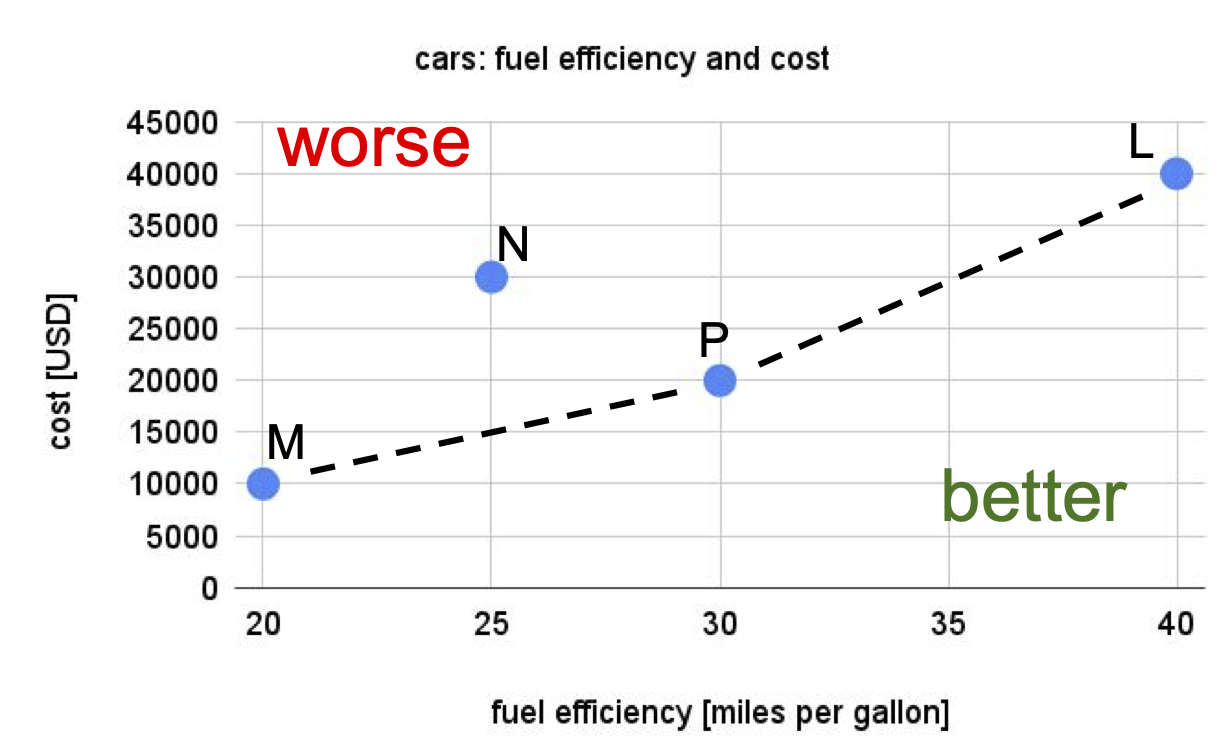
\includegraphics[width=1\textwidth]{images/pareto_frontier_car_options.pdf}
    \caption{Four cars: L, M, N, and P. The buyer's goal is to spend less money (lower on the vertical axis) and get better fuel efficiency (right on the horizontal axis). Choices not on the frontier should be avoided, but that doesn't yield a single result.}
    \label{fig:pareto_frontier_cars}
\end{figure}

Visualizing a Pareto frontier for two quantitative variables is easy, but typically decisions involve more factors. For example, evaluating the trade-off of three quantitative variables like 
passenger capacity, cost, and fuel efficiency creates a surface. With more than three variables visualization is less useful, though the analysis technique still applies. 

Another constraint on using Pareto frontier analysis is that it works well when there are many options relative to the number of variables you are optimizing for. 
The assessment does not work well when there are few choices relative to the number of variables. For example, suppose there are five choices of car and you want high fuel efficiency, sufficient cargo capacity, maximum number of passengers, stylish, low cost, low maintenance, good durability, and high resale value. Then defining a Pareto frontier is less helpful.

For a set of quantitative variables, a Pareto frontier does not account for the relative importance of different variables. Assigning weights to each of these factors merely stretches one axis relative to the other axes. 

There are many possible %decision-making 
% 2023-01-11: Brian Black says to remove redundancy
frameworks besides Pareto frontiers, but in practice a typical bureaucratic decision is ill-informed, has diffuse consequences, delayed impact, and does not affect the decision-maker. In bureaucratic processes there is rarely a formal assessment of options. 
Decisions are rarely recorded. 
Even afterward a decision can be difficult to evaluate for correctness because there are multiple stakeholders.

\textit{Tip}: If the people you want to convince are not swayed by data, then you can augment the \href{https://en.wikipedia.org/wiki/Cost\%E2\%80\%93benefit_analysis}{analysis of costs and benefits} with emotionally-impactful stories. 
\index{Wikipedia!cost-benefit analysis@\href{https://en.wikipedia.org/wiki/Cost\%E2\%80\%93benefit_analysis}{cost-benefit analysis}}
\iftoggle{WPinmargin}{\marginpar{$>$Wikipedia: cost-benefit analysis}}{}

\subsubsection*{Risks of Using Decision Frameworks}

%Decision-making 
% 2023-01-11: Brian Black says to remove redundancy
Frameworks can be attractive to bureaucrats intending to formalize 
\hyperref[sec:process]{processes} 
\marginpar{See page~\pageref{sec:process}.}%
%(see section~\ref{sec:process}) 
and encourage predictability, but there are potential risks to be aware of.  For example, analysis of costs and benefits can decrease the apparent responsibility of the decision-maker. Another risk is that cost-benefit analysis can be used to deflect criticism for an action. 

A good approach for data-driven quantitative analysis involves coming up with a testable hypothesis, pre-registering what actions are to be taken after assessing the results, then performing experiments and collecting data to evaluate the hypothesis. A decision can be characterized as quantitative when based on measurements. For example, before going into a store I set a threshold: I'm willing to spend up to \$30 on a pair of pants. If no pants that I want are available at or below that price then I don't buy pants. 

More commonly, a decision is made, then data is gathered which supports the desired outcome. Forming an opinion and then looking for evidence to back the outcome yields suboptimal results for the organization but maintains the relationships of the decision-maker. The value to the individual using that suboptimal approach is extracted from other members of the organization or subjects of the bureaucracy. 

% https://graphthinking.blogspot.com/2019/01/political-decisions-versus-science.html
To distinguish good data-driven decisions from the more common experiences let's be precise about the other ways decisions get made.
A decision is political when the basis is historical relationships, maintenance or creation of a relationship, or to enable future relationships. 
A decision is subjective when someone else faced with the same scenario would have come to a different conclusion. To avoid the appearance of subjective decision-making or political decision-making, a bureaucrat may frame a decision as ``data-driven." To evaluate which label is relevant, look for measurements and pre-registered actions. 
% https://graphthinking.blogspot.com/2018/06/data-driven-decisions-versus-data.html


Even when a bureaucrat is not intentionally biased towards an outcome, there are many ways to gather evidence -- informal conversations with stakeholders, formal surveys, measuring aspects of the problem. The choice of information gathering is constrained by cost and time, producing incomplete picture of the options. Poor data collection with biased sampling produce biased results. 

Even with valid and representative data measurement, decision-makers can be led astray by poor modeling. A model may use inapplicable techniques or may have implementation bugs.

For all the dangers described above,
%of decision-making methods, 
% 2023-01-11: Brian Black says to remove redundancy
there are worse approaches that do not rely on measurement. People rely on history (if they are aware of it) and perpetuate bad ideas, or take action based on what is best for their career, or decide based on how to accumulate more power, or choose based on what someone else says to do.  

%\subsubsection{Alternative Decision-Making Approaches}
% 2023-01-11: Brian Black says to remove redundancy
\subsubsection*{Alternative Approaches}
Identifying the spectrum of ways bureaucrats make decisions can decrease the surprise when you encounter the approaches in practice. 
\index{decrease surprise!decision-making techniques}
Enumerating the choices of how to make a decision allows for conversation about the pros and cons of each. The spectrum below is ordered from least effective to most effective and is not exhaustive.
\begin{enumerate}
    \item Random selection from the options (e.g., roll of the dice, shake the Magic 8 ball shown in figure~\ref{fig:magic8ball}). The decision-maker is minimizing their involvement. 
    \item Rely on a hunch. The decision-maker is involved with the options but doesn't rely on data. 
    \item Rely on experience, whether yours or someone else's.
    \item Use a \href{https://en.wikipedia.org/wiki/Cost\%E2\%80\%93benefit_analysis}{cost-benefit model} that identified relevant factors and relates them to determine possible outcomes, 
    \index{Wikipedia!cost-benefit analysis@\href{https://en.wikipedia.org/wiki/Cost\%E2\%80\%93benefit_analysis}{cost-benefit analysis}}
    \iftoggle{WPinmargin}{\marginpar{$>$Wikipedia: cost-benefit analysis}}{} then gather data, and analyze to inform the decision.
    \item Make a hypothesis, design an experiment, carry out a test, collect data, and analyze.
\end{enumerate}

Brainstorming aspects of bureaucracy like ``how do decisions get made?" improves your emotional resilience when you encounter instances in your life. Building your Process Empathy involves thinking about how someone else might accomplish an activity. Not what is the best way, but what are all the possible ways. %Instead of cynicism and frustration, compassion and forgiveness. 

\begin{figure}
    \centering
    \includegraphics[width=0.4\textwidth]{images/magic8ball.pdf}
    \caption{Magic 8 ball for decision-making. The least effective method of selecting an option.}
    \label{fig:magic8ball}
\end{figure}

\subsubsection*{Why cost-benefit analysis models are not used}

Applying quantitative models to decision-making may seem a valuable path to optimal outcomes. Improved decision-making that helps stakeholders seems attractive. There are various reasons this approach is not taken. I outline the reasoning here not out of cynicism, but so that you can appropriately respond when confronted with arguments against \href{https://en.wikipedia.org/wiki/Cost\%E2\%80\%93benefit_analysis}{modeling costs and benefits}.\iftoggle{WPinmargin}{\marginpar{$>$Wikipedia: cost-benefit modeling}}{}
\index{Wikipedia!cost-benefit analysis@\href{https://en.wikipedia.org/wiki/Cost\%E2\%80\%93benefit_analysis}{cost-benefit analysis}}
\index{decrease surprise!reasons not to use cost-benefit modeling}%
Decreasing your surprise through the inoculation of exposure enables you to develop counterarguments. 

One reason to avoid cost-benefit modeling is that there is a lot of work to do, so coming up with a model is an \href{https://en.wikipedia.org/wiki/Opportunity_cost}{opportunity cost} -- you have less time available to do ``real work.'' 
\index{Wikipedia!opportunity cost@\href{https://en.wikipedia.org/wiki/Opportunity_cost}{opportunity cost}}\iftoggle{WPinmargin}{\marginpar{$>$Wikipedia: opportunity cost}}{}
Modeling every decision in detail is unrealistic, so triage is needed -- which decisions warrant what degree of investment in analysis. A person inexperienced in modeling decisions will take longer and is more likely to create a bad model. Practice designing models is expensive. Identifying relevant parameters for inclusion in a model is a learnable skill. 

If a person has a bad experience with cost-benefit modeling, they may be less likely to try again with other decisions. Bad experiences can come from using incorrect data, missing a critical variable, picking the wrong scope for a question, implementing the right model with the wrong math, misinterpreting the result, using a model that is too in-depth or not sufficiently deep, or failing to sell the result of an analysis to stakeholders.

Quantitative cost-benefit modeling doesn't account for personalities or organizational politics. The best options advocated for by a model may decrease the decision-maker's power or prestige, or harm relationships. 

A last reason why cost-benefit models are under utilized is the need for measurements. Designing good data collection and then collecting data is costly in terms of time and attention. Because the measurements involve people the data can get perverted by an undesired feedback loop. That concept is called \href{https://en.wikipedia.org/wiki/Campbell\%27s_law}{Campbell's law}. 
\index{Wikipedia!Campbell's law@\href{https://en.wikipedia.org/wiki/Campbell\%27s_law}{Campbell's law}}
\marginpar{$>>$ Folk Wisdom}
\index{folk wisdom!Campbell's law@\href{https://en.wikipedia.org/wiki/Campbell\%27s_law}{Campbell's law}}

\subsubsection*{Decision-Making Delay\label{sec:decision-delay}}

From an outsider's view, what appears as ``organizational inertia'' is the delay of internal decision-making and the delay of dissemination. 
Delay comes from:
\begin{itemize}
    \item Time used by each decision-maker to gather information, arrive at a decision, change processes, share their choice, and justify their choice. 
    %\item Forcing a continuous variable into a discrete set of choices. Typically the number of choices is small. Discrete choices for a continuous variable is a loss of effectiveness.
    % https://dynomight.net/teaching/
    \item Processes designed to detect and counter cheaters and people with malicious intent, whether that means a malicious bureaucrat or malicious subject. 
\item \href{https://en.wikipedia.org/wiki/Analysis_paralysis}{Analysis paralysis} 
\index{Wikipedia!analysis paralysis@\href{https://en.wikipedia.org/wiki/Analysis_paralysis}{analysis paralysis}}\iftoggle{WPinmargin}{\marginpar{$>$Wikipedia: Analysis paralysis}}{}
due to insufficient information or too much information. Another source  of paralysis is a lack of clarity about which framing is applicable.
\item When other people who are needed to carry out the action push back, either in disagreement or seeking clarification. If the impact on profit doesn't exist or is indirect, then justification for action isn't quantitatively obvious. Therefore there's a higher burden for communication.
\end{itemize}

Regardless of the source, delays for decisions are frustrating for stakeholders -- both the decision-makers and the subjects. Your Process Empathy is built on understanding the reason for why delays are expected.
% The following characterization has no consequence
% Decision-making by bureaucrats can be informal or formal, consensus-based or solo. 


\subsubsection*{A Bureaucratic Decision involves many Decisions}

\textit{What may appear a straightforward choice invokes related opportunities and constraints.}

A decision regarding shared resources is actually a collection of interdependent choices. After recognizing the need for a decision, follow-on decisions include identifying the stakeholders (who to include in an analysis) and identifying options. Who is a stakeholder and what options are available are interrelated. Involving more people expands the number of options and the complexity of coordination. Additional choices associated with reducing uncertainty are how much time to spend on the decision, how much information to gather for the decision (see Dilemma~\ref{table:dilemma-personal-gather-data-lots-vs-little}),
\marginpar{See page~\pageref{table:dilemma-personal-gather-data-lots-vs-little}.}%
whether to make the decision or push the decision to someone with more expertise (see Dilemma~\ref{table:dilemma-personal-scope-of-speaking}), or whether to push the decision to someone with more exposure to the consequences.

Most decisions you make as a bureaucrat do not have hard deadlines. Instead, there are trade-offs in the allocation of your attention. Sooner is preferable since the consequence of the decision helps the organization and allows you to focus on other tasks, but delaying allows you to gather more information for a better-informed decision. See 
Dilemma~\ref{table:dilemma-personal-gather-data-lots-vs-little}
\marginpar{See page~\pageref{table:dilemma-personal-gather-data-lots-vs-little}.}%
and \hyperref[sec:dilemma-trilemma]{other related Dilemmas}.


If a bureaucrat relies on consulting an
\hyperref[sec:expertise]{expert},
\marginpar{See page~\pageref{sec:expertise}.}%
%(see section~\ref{sec:expertise} on expertise),
the decision-maker needs to be confident the expert is not  straying outside their area of expertise. For example, I don't rely on a botanist  to tell me how to change the oil in my car. 
Besides knowing their limitations, the expert should be clear about whether their input is a factual summary, a predictive assessment, or a value judgment. This complicates what you as a bureaucrat are interested in when deciding what's the best choice.


\subsubsection*{Transparency of Decision-Making\label{sec:transparency-of-decisions}}

\textit{A decision about decision-making is about what level of accessibility the decision should have before, during, and after the decision.}

% TODO: what's the prescription? This section just enumerates 

Your %decision-making 
% 2023-01-11: Brian Black says to decrease redundancy
process might change if made visible to stakeholders. You may provide more precise justifications or spend more time gathering evidence to support a claim. Strengthening the arguments is beneficial but takes time and resources. 

Frank conversations and exploratory brainstorming need protections to allow participants to be vulnerable. 
This is the motive for the \href{https://en.wikipedia.org/wiki/Chatham_House_Rule}{Chatham House Rule} -- meeting participants can use information from the discussion, but revealing who made a comment is not allowed.
\index{Wikipedia!Chatham House Rule@\href{https://en.wikipedia.org/wiki/Chatham_House_Rule}{Chatham House Rule}}\iftoggle{WPinmargin}{\marginpar{$>$Wikipedia: Chatham House Rule}}{}
The concept of transparency can apply before a decision is issued, while a policy is in effect, or after the consequence (as part of a review). 
Making decisions as part of a transparent process can make participants more risk-averse because of the potential for failure.

People affected by the decisions benefit from understanding how the decisions were made -- this is the reasoning behind  
\href{https://en.wikipedia.org/wiki/Government_in_the_Sunshine_Act}{Sunshine laws} and the 
\index{Wikipedia!Sunshine Act@\href{https://en.wikipedia.org/wiki/Government_in_the_Sunshine_Act}{Sunshine Act}}
\href{https://en.wikipedia.org/wiki/Freedom_of_Information_Act_(United_States)}{Freedom of Information Act (FOIA)}. 
\index{Wikipedia!Freedom of Information Act@\href{https://en.wikipedia.org/wiki/Freedom_of_Information_Act_(United_States)}{Freedom of Information Act}}\iftoggle{WPinmargin}{\marginpar{$>$Wikipedia: Freedom of Information Act}}{}
Even the symbolism of surveillance changes behavior~\cite{2005_Haley, 2007_Burnham}.



% TODO: TRANSITION to hierarchy

  \clearpage% Process and policy
    \subsection*{Hierarchy of Roles\label{sec:hierarchy-of-roles}}


In an ideal situation, sufficient depth and breath for decision making would be embodied in one person. That might not be possible in every situation. One way to resolve this is to identify distinct scopes of responsibility and then assign different members of an organization separate scopes for decision making. Within a decision making scope there may be more work than one person can handle, so a team is formed. That team may have some members focused on tactical work and other members focused on strategy and coordination. Hierarchy within an organization is the formalization of separate decision-making scopes and associated specialization. 

Partitioning knowledge and decision making enables complex work beyond what one person can accomplish and causes friction among members. An expert reporting to a manager knows things the manager does not, and the manager may have context that the expert lacks. Both bureaucrats (the expert and the manager) need to convey their respective understanding and seek the holistic view.

Hierarchical decision making is one option for coordination among alternatives (like consensus), so why is hierarchy so common? Members of an organization gravitate towards hierarchy because it helps define task scope, assigns responsibility, and obviates a need for building consensus. Reaching consensus for every decision would take time and be more burdensome than appointing a person as the decision maker.

\ \\

A hierarchical organization with partitioned knowledge introduces a challenge: the order in which you share information with others matters. Your choices for who to first describe an idea to are your peers, your management, and your subordinates. 
\marginpar{[Tag] Trilemma} 
\index{trilemma!communication priority: peers, management, subordinates}
The people subordinate to you know more about the topic and are exposed to the consequences. Giving them a chance to vet the idea results in a more robust idea and validates their value in the organization. Alternatively, first sharing your idea with management  allows your superiors to provide context you might not be aware off. And choosing to first start the conversation with your peers indicates you value the relationship and decreases the risk of duplicating work.

\ \\

I've included hierarchy in the section on Fundamentals of Bureaucracy, but that does not imply that hierarchy is a required feature of bureaucracy. Hierarchies of bureaucrats are a common \href{https://en.wikipedia.org/wiki/Organizational_structure}{organizational structure} and are worth studying even if not essential to bureaucracy. The relevance of understanding hierarchy is to identify recurring behavior and patterns to leverage.
Organizations of bureaucrats can intentionally work against the use of hierarchy for decisions, but the amount of effort needed to enable alternatives results in hierarchy being a common approach.

The benefits of formal hierarchy include improved capacity for the number of policy decisions made, enabling consistency of decisions, and leveraging specialization of knowledge. 
Hierarchical decision making has costs: higher latency (compared to a signle decider), inconsistency among bureaucrats (dissemination isn't perfect), waste due to inefficiency, and 
\hyperref[sec:unavoidable-hazards]{many others}.
\ifsectionref
described in section~\ref{sec:unavoidable-hazards}. 
\fi
As another example of the potential for harm, hierarchy enables strategic ignorance. Bureaucrats in positions of power can deny having knowledge of improper activity\footnote{L.~McGoey, ``The Unknowers: How Strategic Ignorance Rules the World" (2019)
% review: https://www.tandfonline.com/doi/abs/10.1080/19460171.2020.1768422?journalCode=rcps20
and 
L.~McGoey, ``The logic of strategic ignorance" (2012). DOI 
10.1111/j.1468-4446.2012.01424.x
}. 



The structure of an organization is dynamic, but at each point in time an organization typically has a defined set of roles. Each role is distinguished by different scopes of decision authority. 
Roles are often confused with titles. What matters is the role (scope of decisions) and who reports to whom. The names of teams can be similarly not descriptive.




Roles in an organization are defined by the boundaries of responsibility. The purpose of a role is to minimize conflict, decrease the need for coordination, reduce redundancy, and allow for control of resources. Clear responsibility boundaries enables effective bureaucracy. 


A conventional characterization of an organization's hierarchy involves two criteria: the depth and breadth of the org chart.
The more people a supervisor oversees, the flatter the organization -- that's the breadth of the organization. The depth of the hierarchy is how many layers there are. See the Valve handbook~\cite{2012_Valve} and Joreen's essay~\cite{1972_Joreen} for contrasting views on the merits of an organization's hierarchy. 

A more practical view of an organization's hierarchy also involves two criteria. The two choices of how a hierarchy is shaped are 
1) how many people a supervisor oversees and 
2) how many supervisors a person has. 
Though you might naively expect that an employee has one boss, but that is \href{https://en.wikipedia.org/wiki/Matrix_management}{not a requirement}. A supervisor for a given topic may have many people reporting to them, and a bureaucrat with multiple roles may report to more than one supervisor.

\ \\

Acting as part of a group means ceding part of your autonomy. Hierarchy cedes more of your responsibility and adds expectations about relationships.
The consequence of hierarchy in an organization is that, as a member of the bureaucracy, you do not have full autonomy -- otherwise you would not be a member of the hierarchy. At the same time, you are not under strict control of the organization -- you still have some subjective decision making authority as a bureaucrat.

The person at the top of the hierarchy does not know everything. The person at the top of the hierarchy does not have input on every decision made in the organization. Some autonomy is retained by all members of the bureaucracy.

Independent of the defined roles and titles in an organization's hierarchy, there are a set of implicit roles and a separate social hierarchy of informal influencers and decision makers. Informal influencers in a bureaucracy usually have long relationships with the decision maker or relevant credentials or both. The credentials can be formal (e.g., a \href{https://en.wikipedia.org/wiki/Doctor_of_Philosophy}{PhD}) or informal (demonstrated success on a project). In either case, the decision maker is relying on another person's expertise. 

Another set of informal relations within an organization is mentors and mentees. These relations allow mentors to share institutional knowledge to mentees, and allows people in senior positions to access the novice perspective. 


\ \\

One consequence of hierarchy is a sense of fear felt by people who report to other people. This fear stems from the loss of control (less autonomy) that leaves the person feeling disempowered. 

For example, consider the following relationship. Sue, is perceived to have power over another person, Amy, because Amy gave up some control to Sue. Amy not having full control over decisions triggers the feeling of fear in Amy, regardless of how Sue behaves. Having complete responsibility for decisions also induces anxiety.

If Sue is aware of the potential for this emotional experience, Sue can compensate for Amy's fear by being friendly and receptive towards Amy. Alternatively Sue may exploit or rely on the fear felt by subordinates. Sue not noticing or accounting for Amy's fear does not invalidate Amy's emotional experience.


% Active bystander when the person doing wrong is in a position of authority
% PACT (Probe, Alert, Challenge, Take Action)
% https://mobile.twitter.com/GeorgetownABLE/status/1408498438203969541


% Mintzberg's Coordination Mechanisms
% https://www.youtube.com/watch?v=IZET8VjSifQ

 % subsubsection, so no clearpage
    \subsubsection*{Organizational chart as a Guide and a Lie\label{sec:org-chart-as-guide-and-lie}}

An \href{https://en.wikipedia.org/wiki/Organizational_chart}{organizational chart} 
\index{Wikipedia!\href{https://en.wikipedia.org/wiki/Organizational_chart}{organizational chart}}
(hereafter an ``\gls{org chart}'') identifies formal roles and the formal relations among roles. An org chart is at best a snapshot in time, and more often aspirational than descriptive. In spite of possible deficiencies, an org chart helps outsiders and newcomers understand the scope of responsibilities and interactions.\footnote{The organization chart hasn't always existed. The \href{https://en.wikipedia.org/wiki/George_Holt_Henshaw\#First_organization_chart}{first known org chart} 
\index{Wikipedia!\href{https://en.wikipedia.org/wiki/George_Holt_Henshaw}{George Holt Henshaw}}
was created in the 1850s.}

Org charts are a lie in the sense that undocumented relationships can matter more than the official roles. Org charts fail to capture the informal roles and network of relations that facilitate progress in any organization. Org charts document titles instead of describing roles.

Org charts foster a second separate lie by creating a sense of power dynamics based on visual orientation. For more on this issue see the discussion of~\hyperref[sec:org-chart-orientation]{org chart orientation} on page~\pageref{sec:org-chart-orientation}.
 \clearpage
    \subsection*{Fundamental: Meetings for Coordination\label{sec:meetings-for-coordination}}

In an organization comprised of more than one person, meetings are necessary to facilitate coordination. The coordination accomplished by a meeting can be explicit (verbal or written), or it can be indirect through signaling (who attended the meeting, when the meeting was held, where the meeting was held, or how much notice was provided). 

Not everyone understands that meetings are vital to coordination in a bureaucracy. The following sequence of scenarios illustrates the thinking some bureaucrats use.
\index{decrease surprise!anti-meeting anti-planning}
If you're already convinced of the value of meetings, 
see \hyperref[sec:well-run-meeting]{tips on improvement}\iftoggle{haspagenumbers}{ on page~\pageref{sec:well-run-meeting}.}{.}

\ \\
% https://graphthinking.blogspot.com/2021/07/thought-terminating-concepts-in.html
\textit{Anti-meeting view}: No plan or coordination needed; I just do what you tell me. With this approach, either I will be successful because I worked hard on what my supervisor directed, or I will fail because my supervisor directed me to do the wrong thing.\\
\textit{Potential response by the supervisor}: You are smart, and you're capable of shaping your career. Let's work as a team to improve your effectiveness. \\
\textit{Another potential response by the supervisor}: Is that how you want your career to go? Or do you desire autonomy and creativity?

\ \\
\textit{Anti-meeting view}: No point in making a plan or coordinating because everything changes so often. \\
\textit{Potential response by the supervisor}: But the work has an end goal, right?\\
\textit{Anti-meeting view}:  Yes, so then the plan is to get from where we are now to that end goal. Coordinate as necessary. \\
\textit{Potential response by the supervisor}: And there are no intermediary steps? Milestones?
Is it better to have no plans and just put out fires as a reaction, or to have a plan with contingencies that are subject to change? %To wait for a need for coordination?

\begin{figure}%[H]
    \centering
    % left lower right upper  
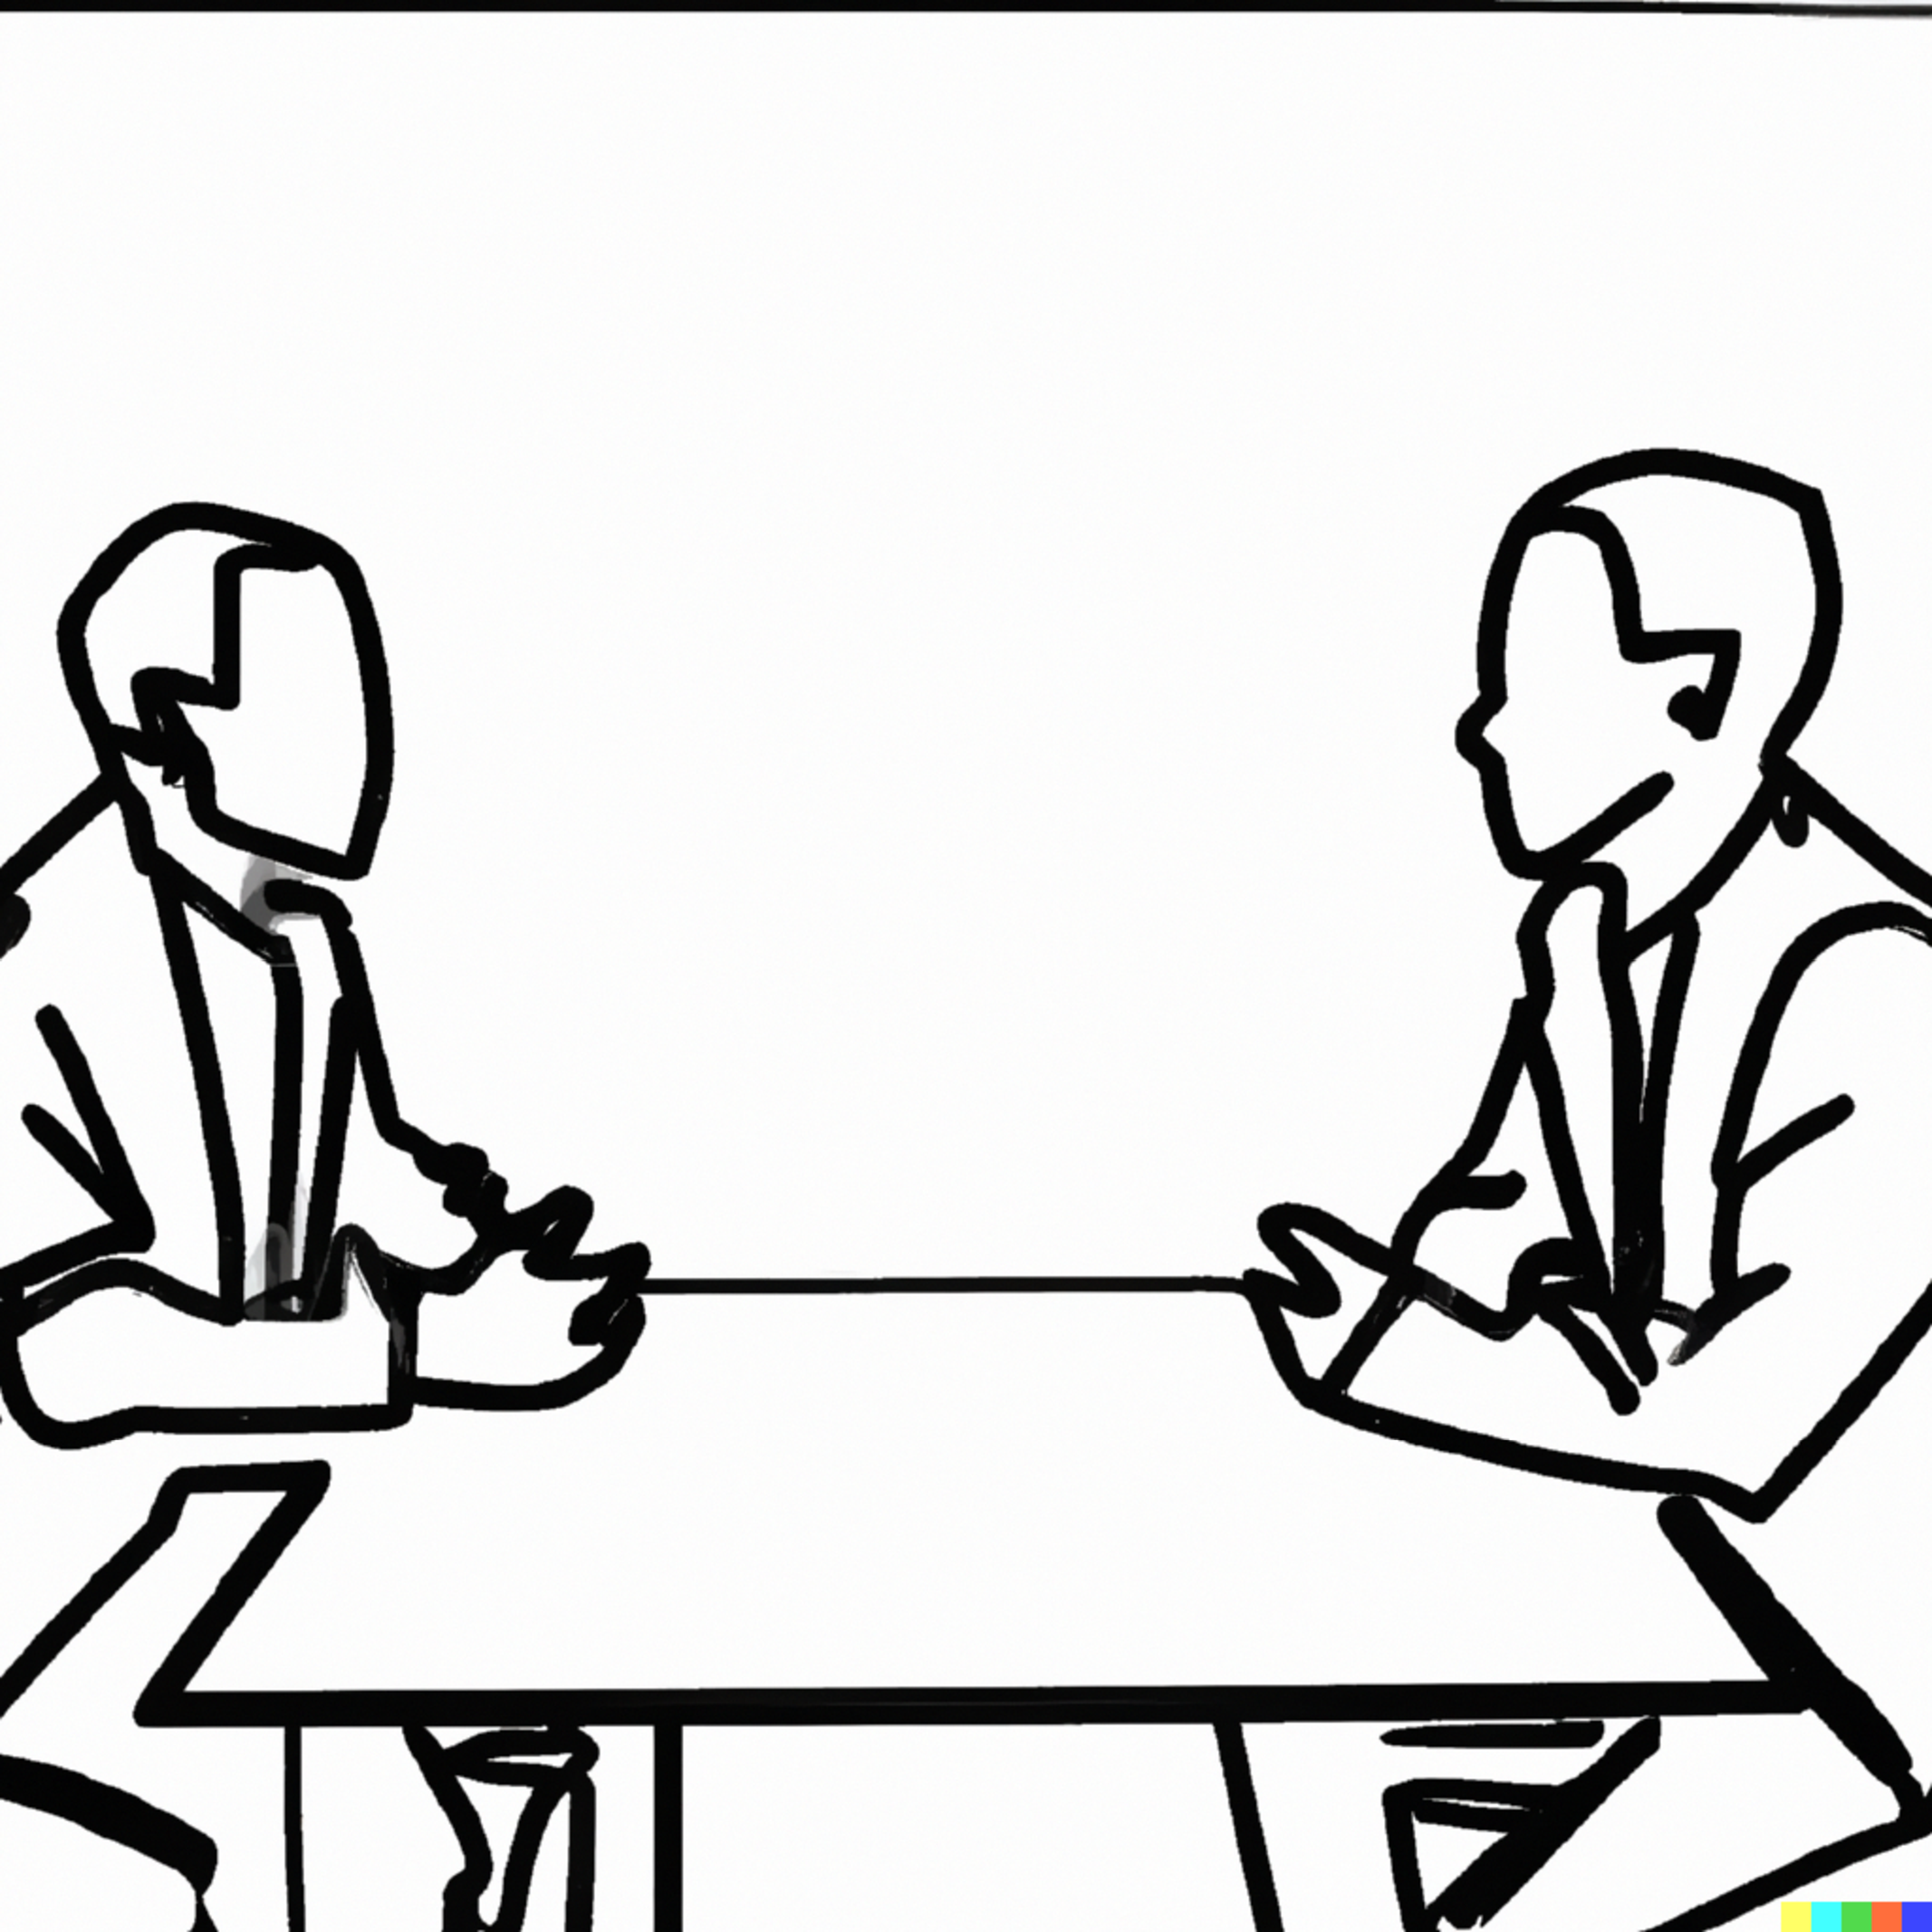
\includegraphics[width=0.6\textwidth,trim={0 .6cm 0 1cm},clip]{images/confrontational_meeting_of_two_people_in_a_conference_room_both_are_seated.pdf}
    \caption{Meeting to discuss the value of coordination. Face-to-face in-person meetings enable participants to convey non-verbal information -- posture, attentiveness, respect, curiosity, distraction.}
    \label{fig:meeting-to-discuss-coordination}
\end{figure}


\ \\
\textit{Anti-meeting view}: What is a plan anyways?\\
\textit{Potential response by the supervisor}: There is value in collaboratively specifying a goal, enumerating tasks that would support the goal, identifying the dependencies among the sub-tasks, and time-binning the dependencies with defined milestones and deliverables. That is my definition of a plan. And having that is more useful than merely reacting.

\ \\
\textit{Anti-meeting view}: Who's plan? Who's relationships? I don't need to come up with that plan, the supervisor already has a plan. Just tell me what the plan is.\\
\textit{Potential response by the supervisor}: That's not as effective as coming up with independent plans and then resolving the differences. There's value in resolving the differences, even though that will cost time and frustration and displace time to enact the plan.


\ \\

Not every team member in a bureaucracy is against planning, or as obstinate about collaboration. 
My intent for sharing these debates is that you will be less surprised when your coworkers raise them. Process Empathy is most relevant when the people you rely on lack Process Empathy.
 \clearpage
    \subsection*{Fundamental: Written Communication\label{sec:written-communication}}

As with hierarchy, written communication is not required for bureaucracy. However, written communication is extremely common and can be helpful. %An artifact of interaction gains value beyond the content.

Paperwork,  \href{https://en.wikipedia.org/wiki/Red_tape}{red tape},
\index{Wikipedia!red tape@\href{https://en.wikipedia.org/wiki/Red_tape}{red tape}}
and modern electronic forms are closely associated with bureaucracy.
Digital reports, spreadsheets, and emails are the current technological artifacts of an organization's bureaucracy. A written record creates evidence about policies, justifications, and decisions regardless of format. %Existence of a record can be used for good or for harm.
Written records are burdensome to create and maintain and search, but they are not intrinsically good or bad. 

Becoming skilled at creating written records is crucial for being an effective bureaucrat. You may have some education on spelling, grammar, and composing essays, but the artifacts of bureaucracy have distinct best practices. For example, plagiarism can be good -- you're being consistent and efficient.  
Chapter~\ref{sec:communication-within-bureaucracy} 
\marginpar{See page~\pageref{sec:communication-within-bureaucracy}.}%
provides advice on effective verbal and written communication in the context of a bureaucratic organization.  \clearpage
    \subsection*{Fundamental: Feedback loops and Ripples\label{sec:feedback-loop-and-ripples}}

%When there is a lack of input from customers or users, then someone has to decide.


A feedback loop exists when a decision-maker experiences the harms and benefits of their decision. Decisions that lack a feedback loop still have consequences for the decision-maker, in that potential future decisions are altered or limited.\footnote{In Street-Level Bureaucracy~\cite{1983_Lipsky} Lipsky discusses feedback loops in chapter~4 on page~40.}


Virtuous cycles and vicious cycles are rare in bureaucratic organizations because there are rarely mechanisms for feedback loops. 
Instead, there are \iftoggle{glossarysubstitutionworks}{\glspl{ripple}}{ripples} -- propagation of consequences for other people's schedules, 
altering what is possible for other people, and creating dependent tasks to be carried out by people other than the decision-maker.


The weak feedback mechanisms for a bureaucrat are reputation (subject to spin)
\index{reputation}
and rarely enforced retroactive accountability in the form of the question, ``What did you know and when did you know it?''
%Reputation is social.
Retroactive accountability depends on written records from meeting notes, emails, agendas, and reports. Reducing the potential for retroactive accountability is one motive for bureaucrats avoiding written records for decisions and policies.


Because of the lack of quantitative feedback loops for bureaucrats, there is significant interest in documenting justification, proactive monitoring, reporting, and retroactive assessment. Each of those activities creates more administrivia.


When there are multiple competing objectives among stakeholders in a 
\href{https://en.wikipedia.org/wiki/Zero-sum_game}{zero-sum}
\index{Wikipedia!\href{https://en.wikipedia.org/wiki/Zero-sum_game}{zero-sum game}}\iftoggle{WPinmargin}{\marginpar{$>$Wikipedia: zero-sum game}}{}
use of resources (my win is your loss), how can you determine what's best? In some domains there are feedback loops to guide progress. When feedback loops are weak or not present,  the most powerful stakeholder (potentially distinct from the biggest or loudest) will dominate. 


\ \\

%****************************************
% https://graphthinking.blogspot.com/2020/01/hierarchy-of-justification.html

Because feedback loops are weak for decision-makers, alternative mechanisms are needed in bureaucracy. A standard approach is the use of approvals and justifications. The strength of justification needed for a given action depends on your relationship with the approver and the potential ripples associated with the action. 

The amount of justification for an approval process should be just enough so that when something goes wrong there's a clear reason why. 

Ordering the quality of a justification
\index{decrease surprise!quality of justification}
\begin{enumerate}
    \item I have no explanation.
    \item This is my opinion.
    \item We've always done it that way (a \href{https://en.wikipedia.org/wiki/Cargo_cult}{cargo cult} in which the underlying reasoning is not understood by participants).
    \index{Wikipedia!\href{https://en.wikipedia.org/wiki/Cargo_cult}{cargo cult}}
    \iftoggle{WPinmargin}{\marginpar{$>$Wikipedia: Cargo cult}}{}
    \item Based on my experience.
    \item I was told to do it this way.
    \item I think this is the best way (no reasoning, but a desire to optimize; optimization criterion undefined).
    \item This way is most effective because X (where X is not quantified, there is a desire to optimize, and there is an optimization criterion).
    \item This way is most effective because X (where X is quantified, there is a desire to optimize, and there is an optimization criterion).
    \item This way is most effective because X compared to other options (where X is quantified, there is a desire to optimize, and there is an optimization criterion).
\end{enumerate}

%****************************************

\ \\

% TODO: need a transition between topics


\subsubsection*{Special interest groups}

% DESCRIPTION
Within bureaucratic organizations, special interest groups care about specific aspects of the shared resource central to the organization. 
Inefficiency can occur when there is a benefit to a small group and the cost is to a larger group.
% TODO? tie in with Public choice theory

The \href{https://en.wikipedia.org/wiki/Social_trap}{social trap}
\index{Wikipedia!\href{https://en.wikipedia.org/wiki/Social_trap}{social trap}}
\iftoggle{WPinmargin}{\marginpar{$>$Wikipedia: social trap}}{}
is ``a conflict of interest or perverse incentive where individuals or a group of people act to obtain short-term individual gains, which in the long run leads to a loss for the group as a whole."
The feedback loop for the diffused value relevant to the organization is weaker than the feedback loop for value to the interest group. 

% PRESCRIPTION
Confronting an individual about a group problem usually results in ``I can't fix everyone else's behavior." Similarly, a team that is benefiting at a cost to the organization is unmotivated to change. A way to productively engage is to get all stakeholders in an in-person meeting. This social pressure, combined with the prompt to find a way to limit harmful behavior, can encourage brainstorming of better approaches. 

\subsubsection*{Spending taxpayer dollars}

As an example of a weak feedback loop, consider the scenario of a government employee deciding how to spend government money.

%\marginpar{[Tag] Story Time; Math}
\index{story time!taxes and spending}
%\begin{storytime}{Taxes and Spending}
\begin{mdframed}[frametitle={Taxes and Spending},frametitlerule=true,frametitlealignment=\centering]
Suppose you are a government bureaucrat and earn \$100,000 with a tax rate of 30\%. Then your tax money sent to the government is \$30,000.
How does that compare to what the government collects in taxes?

For the United States, ``in 2021 the government collected \$4.05 trillion in revenue."\footnote{Government Revenue from the \href{https://datalab.usaspending.gov/americas-finance-guide/revenue/}{U.S. Treasury Data Lab}, 2023.}

That means your taxes of \$30,000 would be
30000/4050000000000 = 0.00000074\% of the tax base for the country.

If you are a federal government bureaucrat and you do not maximize the effectiveness of spending \$1,000,000 of government money, of that misallocated money only \$0.0074, or about one penny, was taxes you paid. The financial feedback loop is weak.

Some federal government bureaucrats earn slightly more, so the cost of wasting \$1,000,000 is more significant.
Federal pay is limited to about \$220,000\footnote{See the Wikipedia entry on \href{https://en.wikipedia.org/wiki/Executive\_Schedule}{Executive Schedule}.
\index{Wikipedia!\href{https://en.wikipedia.org/wiki/Executive\_Schedule}{executive schedule}}
%%%CANTDOINFOOTNOT\marginpar{$>$Wikipedia: Executive schedule}
}, raising the feedback to 2 pennies.
%\end{storytime}
\end{mdframed}

The lack of feedback allows waste to go unfelt. There's no immediate consequence for the decision-maker.
%Waste is indistinguishable from not enough funding or insufficient skills.

\ \\

Example feedback loop:
\begin{center}
\begin{figure}[ht]
    \centering
    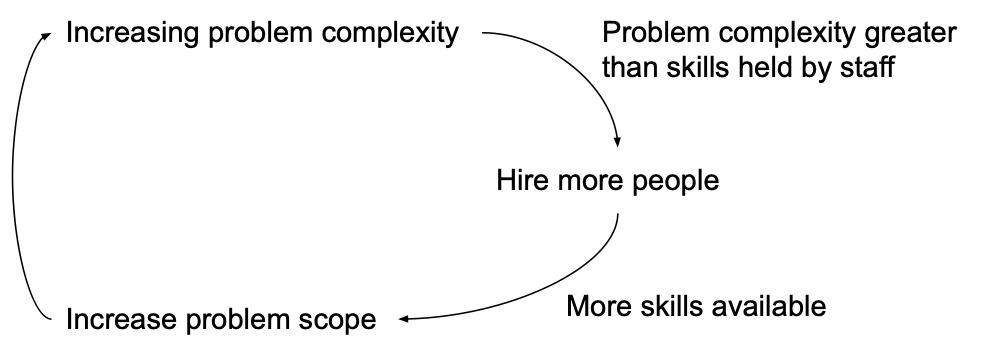
\includegraphics[width=0.8\textwidth]{images/feedback_loop_complexity_and_staffing}
    \caption{Increased complexity requires more staffing to enable specialization. More staff means more skills are available; under-utilized staff skills make room for more scope; more scope adds to complexity.}
    \label{fig:complexity_and_staff_growth}
\end{figure}
\end{center}

\subsubsection{Example feedback loops}%: Security agent making a fair decision}
% https://graphthinking.blogspot.com/2017/09/a-simple-illustration-of-bureaucracy.html
%\marginpar{[Tag] Story Time}
\index{story time!airport security}
\index{exemplar!\href{https://en.wikipedia.org/wiki/Transportation_Security_Administration}{Transportation Security Administration (TSA)}}
%\begin{storytime}{Airport Security Line}
\begin{mdframed}[frametitle={Airport Security Line},frametitlerule=true,frametitlealignment=\centering]
A coworker and I were going through passport control at an airport. 
A \href{https://en.wikipedia.org/wiki/Transportation_Security_Administration}{Transportation Security Administration (TSA) officer} 
%\index{exemplar!\href{https://en.wikipedia.org/wiki/Transportation_Security_Administration}{Transportation Security Administration (TSA)}}
\index{Wikipedia!\href{https://en.wikipedia.org/wiki/Transportation_Security_Administration}{Transportation Security Administration}}
%CANTDOWITHINMDFRAMED\marginpar{$>$Wikipedia: TSA}
was directing passengers into one of two lines. Both lines were long. The length of each line was not equal even though the entrance to the lines was at the same location. Each line terminated at a row of passport-checking agents. Each passport check took a minute. Passport-checking TSA officers operate independently and concurrently.


The TSA officer's perspective is that there are two long lines. Her procedure is two balance the two lines (for fairness). He does this by pointing people into one of the two lines, with her choice driven by which line appears to have room available.

My coworker and I enter the controlled area and are directed into lines by the TSA officer. The officer directs my coworker left and directs me to go right. The TSA officer completed her job.

My coworker in the left line finishes 5 minutes before me. This difference in completion time is frustrating for me.

Because the lines are not of equal length, balancing the start of the line is a suboptimal method. The consequence is that what seems fair to the TSA officer ends up not being fair for people going through the line. The TSA officer had incomplete information -- the lines are not of equal length. Because the TSA officer isn't exposed to the consequence of her approach, she doesn't get feedback on whether her decisions are suboptimal or not.
%\end{storytime}
\end{mdframed}

Lesson: if the people making decisions do not experience the consequences of those decisions, then they have no incentive to improve decision-making.

The person in the longer line feels frustrated. The negative feeling is due to a sense of powerlessness, the situation is recurring, and a better solution is available.

The optimal solution in this situation is to have a single line feeding the multiple TSA passport checkers. A single line eliminates the need for the decision-maker but incurs work to change the status quo.


%\subsubsection{Parking garage}
% from
% https://graphthinking.blogspot.com/2019/07/altering-feedback-loops-to-change.html

%\marginpar{[Tag] Story Time}
\index{story time!parking garage}
%\begin{storytime}{Parking Garage}
\begin{mdframed}[frametitle={Parking Garage},frametitlerule=true,frametitlealignment=\centering]
Bob parks his car in a parking garage every day. 
The parking garage owner charges \$20 per day for people to park their car.

Bob recently found that one of the exit gates for the parking garage is broken. If Bob uses that gate to leave the parking garage, the gate does not function and Bob cannot exit. Then Bob has to call the parking gate operator to request an exception (which is granted) and Bob can then exit that gate, avoiding the \$20 per day charge.

This action (go to broken gate, request exception, avoid charge) has been repeated for a long time (months). Bob's motive is to avoid the \$20 parking charge; the cost is a mere phone call and a minor delay. This cheating behavior harms the parking garage owner's income. However, the parking gate operator, serving as intermediary, insulates the parking garage owner from interaction with the cheater. The cheating behavior is small enough that the parking garage owner may not notice.
%\end{storytime}
\end{mdframed}

Having an intermediary policy enforcer alleviates the need for the garage owner to interact with customers. If the incentives of stakeholders are not aligned then inefficiency goes unchecked. If the parking garage operator's profits are a fixed rate rather than tied to parking charges, then the operator lacks the motive to fix problems.   \clearpage% subsection
  \clearpage
  \section{History of Bureaucracy\label{sec:history}}


Bureaucracy has repeatedly arisen independently in a variety of cultures
\footnote{Wikipedia entry on the \href{https://en.wikipedia.org/wiki/Bureaucracy\%23History}{history of bureaucracy}.
\index{Wikipedia!\href{https://en.wikipedia.org/wiki/Bureaucracy\%23History}{history of bureaucracy}}
}
lasting for timescales that exceed the lifespan of one person\footnote{YouTube video on the \href{https://www.youtube.com/watch?v=B_nsZlcC12g}{History of bureaucracy}.}. That indicates the current situation is not a fluke or coincidence. There is some utility (or pathology) that is consistently recurring. 


Bureaucracy predates writing and language and even humans! Subjective policy enforcement in support of an organization arises in pre-human tribes, visible in groups of modern apes who have to manage access to shared resources~\cite{2016_Suchak}. 



Though bureaucracy is not new, the pervasiveness is. Prior to the industrial revolution the scale of both employment and government were small organizations limited by the speed of communication. For the past 100+ years the size of organizations (commercial and governmental and academia) have grown beyond \href{https://en.wikipedia.org/wiki/Dunbar\%27s_number}{Dunbar's number}. 
\index{Wikipedia!\href{https://en.wikipedia.org/wiki/Dunbar\%27s_number}{Dunbar's number}}
More people participate in more organizations that are more bureaucratic. Driving this increase is the support for more complex products and processes. 

% claim: bureaucracy grow faster than the growth of human population?


 % section
  \clearpage 

\chapter{Bureaucracy in General\label{sec:bureaucracy-in-general}}
{\footnotesize Back to the \hyperref[sec:toc]{Main Table of Contents}}
\minitoc
  \section{Avoiding Bureaucracy is Nearly Impossible}
\iftoggle{shortsectiontitle}{\sectionmark{Avoiding Bureaucracy}}{}

The only situation where bureaucracy might not exist is if you live entirely independently and have no interaction with other people. That means completely disengaging from society. Even then, personal routines are a self-imposed form of bureaucracy, with the roles of policymaker, bureaucrat, and subject collapsed to a single person -- you.

Self-sufficiency and autonomy are attractive alternatives to bureaucracy. The way participants in modern society strive for self-sufficiency is by denying their dependence on modern society. That's a relabeling of selfishness which feels better. 

For the rest of us who operate as members of  society, bureaucracy is necessary for our rights. You validate your name using paperwork, forms, and records. These artifacts are used, in cooperation with other people, to determine your claim of citizenship and associated rights. 
That's a policy that \iftoggle{glossarysubstitutionworks}{\glspl{stakeholder}}{stakeholders} in society agree to. 


Bureaucracy is useful as a response to the \iftoggle{WPinmargin}{\marginpar{$>$Wikipedia: Collective action problem}}{}%
\href{https://en.wikipedia.org/wiki/Collective_action_problem}{collective action problem} -- everyone would benefit from cooperation, but each person has to sacrifice their self-interests.  
\index{Wikipedia!collective action problem@\href{https://en.wikipedia.org/wiki/Collective_action_problem}{collective action problem}}
As long as humans form communities, we will address the challenge of \iftoggle{glossarysubstitutionworks}{\glspl{shared resource}}{shared resources}
 -- whether tangible (e.g., water, land, air) or intangible (e.g., expertise, information). 
That is why bureaucracy is culturally invariant and persistent across time.
Learning to be an effective bureaucrat improves your chances of success in society. 

The specific way society is constructed (democratic, authoritarian, dictatorship, anarchy) is irrelevant -- bureaucracy is still present. Even the libertarian approach of relying on contract enforcement implies some bureaucracy (e.g., forums for resolving contract disputes like a court system, enforcing decisions through violence). 


Not all bureaucracy is due to the state, nor is bureaucracy confined to companies. Parenting involves creating situation-specific requirements for children, with the organization being the family as mentioned in Figure~\ref{fig:family-of-bureaucrats} and the next section 
that describes \hyperref[sec:bureaucracy-early-childhood]{bureaucracy in childhood}.
\marginpar{See page~\pageref{sec:bureaucracy-early-childhood}.}%
Dress codes for sports teams are arbitrary standards. 
Store clerks are bureaucrats, as are website forum moderators.  
Content moderation is the process of enforcing standards. 
%Content moderation is the process of (inconsistently) enforcing arbitrary standards. 
%This mindset even permeates individuals as internalized expectations of policy and enforcement when no one else is present. 

Recognizing instances of bureaucracy enables more skillful interaction, whether as a bureaucrat or subject. The rest of this section illustrates both the view of a person interacting with bureaucracy as a \gls{subject} and the perspective of bureaucrats working within organizations. 




 \clearpage
  \section{Each Phase of Life Involves Bureaucracy}

%\href{https://en.wikipedia.org/wiki/TL;DR}{TL;DR}: 
%\index{Wikipedia!\href{https://en.wikipedia.org/wiki/TL;DR}{TL;DR}}
\textit{Summary}: You have experience with bureaucracy, though you may not have framed the experiences as bureaucratic. Viewing relationships and roles through the lens of bureaucracy explains the limitations of your expectations.

\ \\

In each person's life there are standard milestones: birth, education, work, and death. 
%The relationships associated with each phase are distinct.
Each of these milestones and phases involves bureaucracy. Each phase is a different experience of bureaucracy because the bureaucratic roles change.

Bureaucracy is composed of three roles: the policy creator, the policy enforcer, and the subject (upon whom the policy is inflicted). 
\index{bureaucracy!roles}
These roles can be confounded by oversubscribing the label ``bureaucrat." Who is the bureaucrat and who is the subject depends on the relationship in a scenario. 

For example, a store manager creates a policy, a store clerk enforces the policy, 
\index{exemplar!store clerk}
and the policy is inflicted on the customer. Both the manager and the store clerk would be bureaucrats, while the customer is the subject. In a separate example, someone at corporate headquarters sets a policy, the store manager enforces it, and the policy is inflicted on the store clerk. Then the clerk was the subject of bureaucracy. 


\subsection*{Bureaucracy of Birth\label{sec:bureacracy-of-birth}}
Your birth was marked by getting a name, registering with the state, and initiating medical records. These tasks were administered by bureaucrats (doctors, nurses, and other hospital staff) on your behalf, and you were the subject of the bureaucracy. You had no autonomy or decision-making authority. 

\subsection*{Bureaucracy in Early Childhood\label{sec:bureaucracy-early-childhood}}
Before starting formal education, the bureaucracy of early childhood is inflicted primarily by family members setting and carrying out policies. The organization of bureaucrats is the family, with the shared resources being housing, food, and experience with survival. Other community members or caretakers may also be involved in carrying out the policies of taking care of you. Your decision-making authority as a subject in this bureaucracy was minimal. 

\subsection*{Bureaucrats at School\label{sec:bureaucracy-of-school}}
Once you started the formal education process, new bureaucrats got involved.  The community of bureaucrats could be a public school, a private school, or homeschooling. In any of those cases, the frontline bureaucrat is the teacher. You're not responsible for making policies that other people follow; you are still the subject of bureaucracy.


The expectations of each phase of school (high school, undergraduate, graduate school) are distinct, and they are different from working in a large organization. Your autonomy increases throughout the duration of school. %, and your ability to make policy that effects others grows. 
Your family and teachers are the bureaucrats. You start building informal organizations of friends, and you start to explore policies around social bonding.

Schooling sets a pattern that most students will fall into for the rest of their lives: you were handed a textbook and told to solve a set of problems. That pattern of taking direction can persist for a long time. However, you are not constrained to persist with that limitation. You have the autonomy to do more than what is required. You can find other textbooks that match your interests or are written from a different view. 

You get to choose the book you want, even if you don't get to choose the topic you will be evaluated on. You don't  need to pick just one reference book -- you can review lots of books and figure out which author style best fits you. You can also choose the level of difficulty -- basic and beginner level, or more advanced. You can choose what's best based on your understanding rather than defer to what a class in school is supposed to cover.

As a subject of the education bureaucracy, you can discover how you learn best. This extra effort requires self-reflection: How do you learn? What works best? What didn't work, and why not? What did you learn? What do you wish you had learned?

Another pattern that schooling relies on is single-question decisions with only one right answer. Examples include math problems and multiple-choice tests. Schooling tends to avoid setting up dilemmas or paradoxes for students. Academic problems in the education process are designed to be independent of the people involved or the history of the situation. 


% https://graphthinking.blogspot.com/2013/02/all-little-things.html
%Where you sit in the classroom matters. Being in the front means you will be exposed to fewer distractions, more likely to pay attention.


% https://graphthinking.blogspot.com/2012/09/how-to-not-be-average.html
%How were you taught? Did you have any input on the method?
%Who taught? Did you like them? Were they friendly, knowledgeable, and approachable?


% https://graphthinking.blogspot.com/2012/09/how-to-not-be-average.html
%What resources are available now for you to learn from? Do you like learning?
%you have the freedom to pursue what ever intellectual endeavors you want.


% https://graphthinking.blogspot.com/2011/09/which-skills-are-useful-after.html

% did not prepare me for addressing challenges at work. 
In my schooling I learned how to approach technical issues and develop solutions. That problem-solution paradigm neglects the crucial steps of discovering the problem, isolating the challenge, identifying stakeholders, learning the history of the challenge, and negotiating with stakeholders before trying to address the challenge. 

My schooling led me to emphasize academics over socializing. When I transitioned to professional work, I found social skills and political savvy useful when trying to change organizations and policies. 

Academic problems are intended to be solvable and answers submitted get evaluated. In contrast, working in a bureaucratic organization the challenges are ill-defined, there's no known solution, and the topic is sufficiently complex that you have to collaborate.

% https://graphthinking.blogspot.com/2018/07/the-difference-between-problems-at.html


%\subsection*{undergrad vs graduate}
% education process roles and expectations vary over time

%college, graduate school: friends, teachers, advisors



\subsection*{Military Service Bureaucracy\label{bureaucracy-of-military}}
\index{exemplar!military}
Somewhere between 13 percent\footnote{\href{https://www.cbpp.org/research/federal-budget/where-do-our-federal-tax-dollars-go}{https://www.cbpp.org/research/federal-budget/where-do-our-federal-tax-dollars-go}.} and 20 percent\footnote{\href{https://www.nationalpriorities.org/analysis/2019/tax-day-2019/where-your-tax-dollar-was-spent-2018/}{https://www.nationalpriorities.org/analysis/2019/tax-day-2019/where-your-tax-dollar-was-spent-2018/}.} of the United States federal budget is spent on military, and 
less than 0.5\% of the United States population serves in the military.\footnote{\href{https://www.cfr.org/backgrounder/demographics-us-military}{Council on Foreign Relations}\iftoggle{boundbook}{, https://www.cfr.org/.}{.}}
For those who serve, the military's rigid hierarchy and defined protocols are a distinct experience compared to school or work. Transitioning from military to civilian life can present a dissonance for service members used to the chain of command and clearly defined orders. 

While you are in the military the hierarchy and use of inefficient policies feel stifling. Once out of the military you may reflect fondly on the clarity of orders compared to the vagaries of social politics.  

\subsection*{Working in a Bureaucratic Organization\label{sec:bureaucracy-of-work}}
%Within the employment phase of life, there are pairs of events which may apply: hiring or getting hired; firing, getting fired, or quitting. 

%Employment: managers above you, peer employees, people you manage are all members of an organization. 


Organizations with communal workspaces have \glspl{shared resource}: bathrooms, conference rooms, storage areas, and kitchen areas with fridges and microwaves. Each of these incurs policies of use. Unlike being a student at school, you may find yourself responsible for developing and enforcing policy. 

As an example of workplace policies, consider the following scenario. 
%\marginpar{[Tag] Story Time}
\index{story time!bathroom smells}
%\begin{storytime}{The Bathroom Stinks}
\begin{mdframed}[frametitle={The Bathroom Stinks},frametitlerule=true,frametitlealignment=\centering]
The bathroom at work sometimes smells, so I'm a nice person and bring a scented air freshener. Unbeknownst to me, that triggers asthma or an allergic reaction in one of my coworkers. Because of this a policy gets created so this mistake doesn't happen again. 

Signs are posted. Violations are reported to management even if no one has a physical reaction to the air freshener.
%\end{storytime}
\end{mdframed}

Policies are often created in response to specific incidents. This intent can be helpful (promulgating lessons learned is efficient) or unhelpful (when policies are an overreaction). 

\subsection*{Healthcare and Death\label{sec:bureaucracy-of-death}}
Medical care alters our life, and a lot of money is spent on medical care: 25\% of the federal budget in the United States.\footnote{\href{https://www.cbpp.org/research/federal-budget/where-do-our-federal-tax-dollars-go}{https://www.cbpp.org/research/federal-budget/where-do-our-federal-tax-dollars-go}.} Understanding the bureaucracy of healthcare is outside the scope of this book, but your role in the bureaucracy is helpful to understand.

Doctors, nurses, and other staff are bureaucrats; you are the subject; the hospital or clinic is the organization. 

\ \\
To illustrate bureaucracy of a large organization, consider the importance of toilet paper at a hospital. 
%\marginpar{[Tag] Story Time}
\index{story time!toilet paper at hospital}
%\begin{storytime}{Restocking Toilet Paper}
\begin{mdframed}[frametitle={Restocking Toilet Paper},frametitlerule=true,frametitlealignment=\centering]
If you go to a hospital, use the bathroom, and find there is no toilet paper, that would indicate a deficiency of the hospital.

The \textit{holistic view} is that someone didn't refill the toilet paper. Since the person who usually restocks toilet paper wasn't also a user, they aren't directly affected by the lack of toilet paper.

A routine is needed for checking the availability of toilet paper in bathrooms. 

The \textit{perspective of the purchasing manager} is that money spent checking the status of toilet paper is money not spent on the hospital's primary mission: improving the health of community members.

Minimizing checking of toilet paper is important for the organization's reputation, so a feedback mechanism is instituted: a phone number is posted in the bathroom so users can send a text regarding bathroom status at the hospital.

The \textit{perspective of the janitor} is that my routine used to be to go to each bathroom after normal business hours and refill toilet paper. Now I have to do that and be on-call when someone alerts management that service is needed. My responsibilities increased but my pay did not.

%\end{storytime}
\end{mdframed}

%\ \\

%Death can invoke both the medical system and the government. 

%\ \\


%All of these roles and relationships involve 

Bureaucracy is a set of subjectively administered policies within an organization. By recognizing the role of bureaucrats you can identify what is negotiable. 
 \clearpage
  \chapter[Alternatives to Bureaucracy Don't Work]{Alternatives to Bureaucracy Don't Work\label{sec:alternatives-to-bureaucracy}\iftoggle{shortsectiontitle}{\chaptermark{Alternatives to Bureaucracy}}{}}
\iftoggle{shortsectiontitle}{\chaptermark{Alternatives to Bureaucracy}}{}

% LONG1 shows up in the TOC
% LONG2 is the section title


\textit{This Appendix does not contain prescriptions for the practicing bureaucrat. This content may be of interest to theoreticians.}

A common refrain for participants in an organization is ``Can't I just do the work?'' with the implicit disinterest in coordination and administrivia. This section explores a few alternatives to bureaucracy. These thought experiments illustrate the na\"ive intent and the practical deficiencies of each alternative.

The models of bureaucracy below are all imprecise because they are analogies. The consequence of imprecision is wasted effort. Using a precise and accurate definition of bureaucracy enables improved effectiveness for the work you invest.


% https://graphthinking.blogspot.com/2021/02/how-to-have-efficient-bureaucracy.html

\subsection*{\textit{Alternative}: Efficient Bureaucracy}

In an ideal scenario with no inefficiency, everyone comes to the same conclusion when presented with the same information regarding management of shared resources. Efficient bureaucracy requires each person to know the skills of everyone else so that anyone can act as an expert in any field. 

In this scenario the 
\href{https://en.wikipedia.org/wiki/Overhead_(business)}{overhead cost} 
\index{Wikipedia!overhead, business@\href{https://en.wikipedia.org/wiki/Overhead_(business)}{overhead, (business)}}
of building consensus becomes unnecessary. There is no need to fight over resources (e.g., money, staffing) and no need to fight over what the direction of the organization should be. In this model of efficient bureaucracy based on everyone having the same view, a potential problem is the lack of diverse views needed to enable resilient organizations.

\ \\

While that idealized scenario is unrealistic, it points to how to improve bureaucratic efficiency. Each bureaucrat should have access to the same information (transparency). 
Each bureaucrat should apply the same 
\href{https://en.wikipedia.org/wiki/Decision-making}{decision-making}
\index{Wikipedia!decision-making@\href{https://en.wikipedia.org/wiki/Decision-making}{decision-making}}
process consistently (documented processes and policies).
Each bureaucrat should have the same incentives (fair policies).

The unrealistic model of efficient bureaucracy also points to why bureaucracy is inefficient in predictable ways:
\begin{itemize}
    \item Not everyone has the same information.
    \item Processes are applied inconsistently.
    \item \hyperref[sec:motivations]{Incentives vary} among bureaucrats.
    %(see section~\ref{sec:motivations}).
% https://graphthinking.blogspot.com/2017/03/what-slows-down-bureaucracy.html
    \item Bureaucrats and Subjects use imprecise language.
    \item Decision-makers use opinions and experience rather than collect data and analyze data.
    \item People prioritize putting out fires rather than attacking critical issues.
    \item People do not respond quickly (or at all) to communications (e.g., email, phone, meetings). See the section on \hyperref[sec:slowing-communication]{slow communication}.
    \marginpar{See page~\pageref{sec:slowing-communication}.}
    \item Participants are late to meetings.
    \item \hyperref[sec:scope-creep]{Scope creep} 
    \marginpar{See page~\pageref{sec:scope-creep}.}%
    for projects incurs unnecessary work.
    \item Planned scope and actual scope are mismatched  (due to staffing or skills).
    \item Teams work in silos and create redundancy.
% https://graphthinking.blogspot.com/2017/03/progress-in-spite-of-better-ways.html
    \item Bureaucrats and Subjects lie and employ other dark patterns (not addressed in this book).
    \item People make mistakes.
    \item Each person's reference experiences are unique.
\end{itemize}
By identifying why bureaucracy is inefficient you can actively work to remedy each of the above aspects. 

\ \\

Consider the following 
\href{https://en.wikipedia.org/wiki/Thought_experiment}{thought experiment}. 
\index{Wikipedia!thought experiment@\href{https://en.wikipedia.org/wiki/Thought_experiment}{thought experiment}}\iftoggle{WPinmargin}{\marginpar{$>$Wikipedia: thought experiment}}{}
%What if everybody in a bureaucracy were the same?
What if everybody in a bureaucracy had a different opinion? How would consensus be arrived at? 
\marginpar{$>>$ Thought Exercise}
Can an organization operate without having to agree on every decision? 



\subsection*{\textit{Alternative}: Perfect Bureaucracy}

The definition of ``perfect bureaucracy'' depends on who provides the perspective. The following explores both the subject's view and the bureaucrat's view. 

From the perspective of the subject of a bureaucratic organization, perfect bureaucracy means many things: minimizing the time a subject waits on a decision, getting perfectly correct decisions, decisions being consistent across subjects (Dilemma~\ref{table:dilemma-subject-consistency-per-situation})
\marginpar{See page~\pageref{table:dilemma-subject-consistency-per-situation}.}%
and circumstances (Dilemma~\ref{table:dilemma-personal-policy-consistency-across-cases}), decisions take into account all relevant factors, and there is zero cost to the subject (Dilemma~\ref{table:dilemma-subject-transparency}). 
\marginpar{See page~\pageref{table:dilemma-subject-transparency}.}%
Any situation deviating from those expectations is a noticeable detriment to the subject, leading to a negative reference experience of bureaucracy. 

Never mind that the desires are unreasonable and conflicting. In a real (i.e., imperfect) bureaucracy, subjects have a negative or neutral experience. Positive interactions with bureaucracy are rare and are regarded as abnormal.

Perfect bureaucracy for a bureaucrat means all information is available, information is immediately available, and there is no moral ambiguity (i.e., each answer is objective). Trade-offs become trivial and the emotional toll of the work goes to zero. Then the bureaucrat can serve subjects (an emotionally rewarding prospect). 

This job in a perfect bureaucracy might feel hollow if all decisions are obvious. In a real (imperfect) bureaucracy, the typical experience is negative or neutral, punctuated by glimpses of satisfaction. 

\subsection*{\textit{Alternative}: Everyone does their own thing -- No Coordination, No Bureaucracy}
The scenario involving minimal bureaucracy is a single person working on a single task that does not last long (a few minutes), is relatively easy (cognitively, physically, and emotionally), and does not recur. In that situation, building consensus is irrelevant and no process is required. Even then, it is often the case that this simple task involves using shared limited resources --  essentials like water, air, and land. If your task involves use of those things, then how is fair use determined among consumers?

For simplistic tasks the concept of community-imposed limits to access 
\iftoggle{glossarysubstitutionworks}{\glspl{shared resource}}{shared resources}
%\iftoggle{glossaryinmargin}{\marginpar{[Glossary]}}{} 
is not trivial. When there are no policies to constrain access, violence is used to determine allocation of shared resources.

Most of your actions occur beyond the limits of simplicity and thus incur some concept of \gls{process}
\iftoggle{glossaryinmargin}{\marginpar{[Glossary]}}{}%
(breaking a task into subtasks). Staying with the context of one person, a complex task can benefit from being broken into subtasks. Sometimes the order of the subtasks matters, so we need to track the dependencies. A recurring multi-step process with documentation is starting to have features of bureaucracy but lacks the need for consensus. 


If one person lacks the skills relevant to a multi-step process, they may engage another person to help. The interaction occurs on a spectrum from informal (anarchy) to formalized in a contract (\href{https://en.wikipedia.org/wiki/Libertarianism}{libertarian}).
\index{Wikipedia!libertarian@\href{https://en.wikipedia.org/wiki/Libertarianism}{libertarian}}\iftoggle{WPinmargin}{\marginpar{$>$Wikipedia: libertarian}}{}%
If the parties working on the task fail to reach a consensus, what is the recourse? Choices include physical violence, threats, or involving a third party (e.g., a court with lawyers and judges). 


If a community wants to manage access to shared resources, how is that policy decided?  Building consensus is relevant, but what is the process for establishing consensus? 
\href{https://en.wikipedia.org/wiki/Nepotism}{Nepotism},
\index{Wikipedia!nepotism@\href{https://en.wikipedia.org/wiki/Nepotism}{nepotism}}\iftoggle{WPinmargin}{\marginpar{$>$Wikipedia: Nepotism}}{}%
cultural norms, and 
\href{https://en.wikipedia.org/wiki/Religion}{religious practices}
\index{Wikipedia!religion@\href{https://en.wikipedia.org/wiki/Religion}{religion}}
served this role before the dominance of bureaucracy. 


\subsection*{\textit{Alternative}: Limit Bureaucracy to a Single Decider\label{sec:single-decider}}

Since bureaucracy is distributed knowledge and distributed decision-making, it could be replaced by centralized knowledge and centralized decision-making. If we are going to live in a society and coordinate shared resources, what if we had a single person deciding? How fast could that be? Good decisions are not instantaneous. To understand latency in decision-making let's use the
\href{https://en.wikipedia.org/wiki/OODA_loop}{OODA loop} 
\index{Wikipedia!OODA loop@\href{https://en.wikipedia.org/wiki/OODA_loop}{OODA loop}}\iftoggle{WPinmargin}{\marginpar{$>$Wikipedia: OODA loop}}{}%
model. 

OODA stands for Observe, Orient, Decide, Act. OODA applies to individuals as well as teams and organizations. 
% https://graphthinking.blogspot.com/2016/03/how-to-evolve-organization-community-or.html
The input for the OODA model is to observe and the output is to act. Observing and acting are measurable; the ``orienting" and ``deciding" phases are not as easy to measure. The ``orient" phase requires labeling data received in the ``observe" phase and connecting that information to what is already known.

How quickly could a single decision-maker apply the OODA loop for arbitrary questions about \iftoggle{glossarysubstitutionworks}{\glspl{shared resource}}{shared resources} accessed by a community? Three minutes is not much time to gather information and share it with the relevant people, but let's set that as a lower bound.
\marginpar{$>>$ Math}
If a single decision takes three minutes, then in a ten-hour work day that's a max of $(10*60)/3 = 200$ decisions per day. If this decider works 300 days out of the year, that gets us to 60,000 decisions per year. While 60,000 decisions sound like a lot, that limits how large the community could feasibly be, and the complexity of the decisions is limited. 

Everyone has to talk to this decider directly since there's no bureaucracy to gather or share the information. The diversity of questions regarding shared resources would be challenging to answer well.

Within the constraint of a single decider, we can't just automate everything because carrying out the automation requires staff to enact. 
\index{automation!challenges of}
Automation isn't free -- it requires creation and maintenance. Unless the same person making the decisions is also creating and maintaining the system, there will be multiple people in an organization.


\href{https://en.wikipedia.org/wiki/Monarchy}{Monarchies} 
\index{Wikipedia!monarchy@\href{https://en.wikipedia.org/wiki/Monarchy}{Monarchy}}\iftoggle{WPinmargin}{\marginpar{$>$Wikipedia: Monarchy}}{} 
and 
\href{https://en.wikipedia.org/wiki/Dictator}{dictatorships}
\index{Wikipedia!dictator@\href{https://en.wikipedia.org/wiki/Dictator}{dictator}}
at first glance seem to rely on a single decider. This is a simple model to understand, but addressing all the edge cases for a large society is difficult. A single decider doesn't scale for the number of decisions needed, so the decider then appoints bureaucrats to subjectively enforce policies. 

From this thought experiment we conclude that avoiding bureaucracy by relying on one person doesn't scale. More people are needed to develop and carry out policies. 


%\subsection*{Complexities of more than one Bureaucrat}

% https://graphthinking.blogspot.com/2019/07/first-principles-analysis-of-creating.html

If there's more than one person in an organization, then communication for coordination takes time. That's the ``orient'' phase of the OODA loop. Time spent orienting decreases the decision throughput of the organization.



\subsection*{\textit{Alternative}: Avoid Bureaucracy and Just use Common Sense}
\textit{Claim}: Everything would go smoothly if each person used common sense.
\marginpar{$>>$ Fallacy}

Common sense relies on your reference experiences, cultural norms, incentives, emotional state, and a lack of psychological defects. These aspects are particular to each person in an organization. This gives rise to the observation that 
``common sense is not so common." 
\marginpar{$>>$ Folk Wisdom}
\index{folk wisdom!common sense is not so common}

There are multiple origins of what gets considered to be common sense:
\begin{itemize}
\item Cultural norms. This is what I think everyone else does or thinks.
\item Personal \gls{reference experience}. I've done it this way before.
\item A prescribed action seems obvious.
\end{itemize}

\ \\

Proponents of commonsense who work in existing hierarchical bureaucracies may advocate the removal of non-workers (i.e., management). That may sound like a worker's paradise, but then who coordinates activities when the number of people involved is more than any one member can track (above 
\href{https://en.wikipedia.org/wiki/Dunbar\%27s_number}{Dunbar's number} of about 150 people)?
\index{Wikipedia!Dunbar's number@\href{https://en.wikipedia.org/wiki/Dunbar\%27s_number}{Dunbar's number}}\iftoggle{WPinmargin}{\marginpar{$>$Wikipedia: Dunbar's number}}{}

\ \\

To illustrate the dissonance motivating common sense, consider the following. 
Changing a burnt-out light bulb at home takes me only a few minutes. I've done that many times. Why is that task so hard in an organization?

%\marginpar{$>>$ Story Time}
\index{story time!changing a lightbulb}
%\begin{storytime}{Changing a Lightbulb}
\begin{mdframed}[frametitle={Changing a Lightbulb},frametitlerule=true,frametitlealignment=\centering]
In a large organization comprised of specialized roles, an office worker sees a bulb is out. Rather than go to a nearby hardware store and buy a replacement, they notify their manager who notifies the building supervisor who submits a request to the maintenance team. 

The maintenance service desk team then schedules the repair. An order of 1000 replacement bulbs was made last year and there are some still available in storage. A maintenance team is assigned to the task and deployed to replace the bulb. 

First the maintenance team goes to the storage facility to get a ladder and multiple bulbs of multiple models. The team has to sign out the bulbs from storage so inventory can be tracked (because of prior incidents of theft). A team is needed because solo use of the ladder is prohibited (for safety, also born out of previous incidents). Multiple bulb models are needed because which model is required is unspecified in the service ticket. Having multiple bulbs available decreases the need to go back to storage. 

Once on site, the maintenance staff finds the bulb is a new type and needs to be ordered. Maintenance team notifies the supervisor. The building manager files a new maintenance request.
%\end{storytime}
\end{mdframed}

This is the efficiency of specialization of roles. If you don't like it, you could go to the hardware store, buy a bulb, rent a ladder, install the bulb, and return the ladder.

% https://graphthinking.blogspot.com/2021/09/why-is-everything-so-hard-in-large.html

\subsection*{\textit{Alternative}: Completely Avoid Bureaucracy}
The phrasing of avoidance is more precisely worded by replacing ``bureaucracy" with ``coordination of stakeholders." If you avoid coordination of stakeholders, you either are constrained to only work on tasks that involve one person, or you get random (uncoordinated) interactions. 

\subsection*{\textit{Alternative}: Minimize Bureaucracy}
Again, try replacing ``bureaucracy" with ``coordination of stakeholders." The goal of ``minimizing coordination" probably isn't the real objective. To be more precise, a specific objective might be ``minimize time spent executing the task" (which takes a lot of coordination before the task execution) or ``minimize the level of distraction to stakeholders" (chunk the coordination time, e.g., a meeting). Another strategy for minimizing bureaucracy is to reduce the number of stakeholders involved. For a given task complexity, this means having smarter people who have more skills. See Figure~\ref{fig:complexity-and-size} for a quantitative illustration of the trade-off. 


% \begin{figure}
% \centering
% \includegraphics[width=0.9\textwidth]{images/people-per-task-for-skill-level.pdf}
% \caption{A task that one smart person can do might take two  people that are not as smart. This concept applies to any task size and any population of workers. In this diagram three levels of task complexity are shown. As task complexity increases, the size of the team needs to grow with intelligence held constant. The growth may be less if the team members are brilliant. Those brilliant people cost more and there are fewer of them available.}
% \label{fig:complexity-and-size}
% \end{figure}


\subsection*{\textit{Alternative}: Automation of Processes to Displace Bureaucracy\label{sec:automation}}

The role of automation is to make interactions more predictable, faster, and to handle more of them. Automation does not eliminate bureaucracy; automation obfuscates  subjective decisions and limits the ability to negotiate with decision-makers.
%Automation and computers merely obfuscate processes and make negotiation more challenging. 

Hoping that modern technology will eliminate or reduce bureaucracy is not a shortcut to progress. 
Even with faster decisions and fewer humans, there is still reliance on humans to make decisions and design processes.

% https://graphthinking.blogspot.com/2019/07/bureaucracy-is-social-process-executed.html
There are benefits to automation, and automation can be enacted to minimize harm to bureaucratic subjects. Automated systems can be made more transparent by including documentation about what is happening, why, and what's next.
\index{automation!benefits of}
\marginpar{$>>$ Actionable Advice}%
\index{actionable advice}%
Documentation helps  bureaucrats and subjects identify when assumptions made in the automation are incorrect. 


There are indicators of when to transition from a manual bureaucratic process to a more automated approach:\footnote{\href{https://xkcd.com/1319/}{https://xkcd.com/1319/} -- the risks of investing in automation.}
% https://graphthinking.blogspot.com/2019/07/cost-of-creating-and-supporting.html
\index{automation!when to}
\index{xkcd!xkcd.com/1319@\href{https://xkcd.com/1319/}{1319}}
\begin{itemize}
    \item The process to be automated is stable.
    \item The expected lifespan for the process -- how long the process will be needed -- is  longer than the time to enact the automation.
\item The process logic relies on objective evaluation criteria.  
\item The process is frequent.
\item The cost of automating (both the initial creation cost and the maintenance cost) is a savings over the manual implementation.
\end{itemize}


\subsection*{\textit{Alternative}: Market-based Approach}
% https://graphthinking.blogspot.com/2017/09/market-friction-and-bureaucratic.html

There is an alternative to bureaucracy that features a decentralized approach to complex tasks and avoids reliance on consensus: \href{https://en.wikipedia.org/wiki/Market_(economics)}{markets}.
\index{Wikipedia!market@\href{https://en.wikipedia.org/wiki/Market_(economics)}{markets}}

An oversimplified definition~\cite{2023_Kenton} is ``A market is a medium that allows buyers and sellers of a specific good or service to interact to facilitate an exchange." 
In practice, there is market friction~\cite{2021_Downey, 2011_Matouschek}: ``trading is always associated with certain costs or restraints."

The sources of friction in a market include
\begin{itemize}
    \item Commissions on trades.
    \item Taxes (needed to fund contract enforcement organizations).
    \item Uncertainty in hiring.
    \item Constraints on firing labor.
    \item Search cost in exploring the available opportunities.
    \item Risk uncertainty.
    \item Cost of creating contracts.
    \item Cost of insurance.
\end{itemize}
Market friction and bureaucratic inefficiency are similar~\cite{1937_Coase, 2010_economist}.


Complex tasks at a societal scale range from manufacturing advanced computer chips, to creating and distributing critical medicine, to immigration and border enforcement. 
If a society wants to carry out a complex task involving multiple people, then coordination of effort is required. The coordination can be explicit (in the form of a bureaucracy) or implicit (via a market).  Bureaucracy is one response to the complexity of a problem being solved.


\ \\

Regardless of whether a bureaucratic or market-based approach is used to mediate access to \iftoggle{glossarysubstitutionworks}{\glspl{shared resource}, }{shared resources, }%
% https://graphthinking.blogspot.com/2017/09/market-friction-and-bureaucratic.html
distributed knowledge and distributed decision-making are hindered by aspects like
%\begin{itemize}
limited bandwidth between people participating in the coordination,
non-zero latency of information between people,
the cost of getting data,
and
the cost of analysis of data.
%\end{itemize}
Due to these factors, suboptimal decisions get made. See  %section~\ref{sec:dilemma-trilemma} 
the discussion of 
\hyperref[sec:dilemma-trilemma]{dilemmas}
\marginpar{See page~\pageref{sec:dilemma-trilemma}.}%
for specific examples of trade-offs.

\ \\

The objective and quantified concept of money creates accountability that distinguishes commercial businesses from bureaucracy. Money as a metric is common to all participants within the business and with external stakeholders. 

As with government bureaucrats, commercial businesses have employees who make subjective decisions and enforce policies. Unlike government bureaucracy, in business there is a common metric for feedback: money. This distinction between business and government is not as clear as you might expect since the feedback mechanism does not apply to all members of a business. An effective commercial bureaucrat may rely on the success of other employees rather than a direct interaction with customers. Business employees may take action that is hard to quantify with respect to profits and losses.

Companies are motivated by financial profit, whereas bureaucracies like prisons, schools, hospitals, governments, and militaries  consume and spend money, but money isn't the goal. When faced with a decision, bureaucrats are not guided by which will generate more profit~\cite{2012_Wilson}.

\subsection*{\textit{Alternative}: Adhocracy instead of Bureaucracy}
% https://graphthinking.blogspot.com/2017/09/complex-tasks-necessitate-bureaucracies.html

\href{https://en.wikipedia.org/wiki/Adhocracy}{Adhocracy} 
\index{Wikipedia!adhocracy@\href{https://en.wikipedia.org/wiki/Adhocracy}{adhocracy}}%
\iftoggle{WPinmargin}{\marginpar{$>$Wikipedia: Adhocracy}}{}% 
(also called Tiger Teams)
\index{Wikipedia!tiger team@\href{https://en.wikipedia.org/wiki/Tiger_team}{Tiger team}}
has been proposed in reaction to the prevalence of bureaucracy in organizations. To enact Adhocracy a team of diverse experts is assembled to tackle a complex challenge of limited duration.
While this may be enough for short-duration tasks, if the challenge lasts more than a day or two there will be new issues beyond the original challenge:

\begin{itemize}
    \item What happens to the work that was previously being done by the members of this team?
    \item Who pays the salary for this labor?
    \item Who calculates the payroll?
    \item Who pays the rent for facilities used by the team?
    \item Who does the maintenance of facilities and equipment?
    \item Who cleans the facility?
    \item Does risk incurred mean insurance is needed?
\end{itemize}
To address these questions that are out-of-scope for the complex challenge, you can either use a market-based approach or build a bureaucracy. 

\subsection*{\textit{Alternative}: Consensus Algorithms}

In the description of a \hyperref[sec:single-decider]{single decider}
\marginpar{See page~\pageref{sec:single-decider}.}%
%section~\ref{sec:single-decider} 
the solution was to centralize decision-making and knowledge. The decentralized approaches are market-based or bureaucratic. Another approach to distributed decision-making is to use consensus algorithms. Modern algorithms like
\href{https://en.wikipedia.org/wiki/Paxos_(computer_science)}{Paxos} and
\index{Wikipedia!Paxos@\href{https://en.wikipedia.org/wiki/Paxos_(computer_science)}{Paxos algorithm}}%
\iftoggle{WPinmargin}{\marginpar{$>$Wikipedia: Paxos}}{}%
\href{https://en.wikipedia.org/wiki/Raft_(algorithm)}{Raft}%
\index{Wikipedia!Raft@\href{https://en.wikipedia.org/wiki/Raft_(algorithm)}{Raft algorithm}}%
\footnote{For a tutorial on Raft see \href{https://raft.github.io/}{https://raft.github.io/}.} are widely used for various computer-based tasks. 

Although these algorithms are reliable even when the underlying mechanisms are faulty, the algorithms are not enacted using humans. Humans are unreliable, but more importantly humans game the rules and processes of systems rather than operate within the constraints. Also, relying on an algorithm neglects the feature that humans can adapt to unforeseen circumstances.

\subsection*{\textit{Alternative}: Elected Representatives}
Governments are composed of politicians and bureaucrats. (Government isn't the only place bureaucrats appear, but for this section we'll focus on government.)

The concept of political representatives is easier to understand. A politician is just one person acting on behalf of other people. Members of the community get a vote in who that representative is.
In contrast, the emergent behavior of bureaucracy is more challenging to understand: many people are involved (which inhibits creation of an explanatory narrative) and subjects of bureaucracy do not appoint the bureaucrats. 

% why not make the entire system out of politicians?
Suppose that instead of a bureaucracy all members of an organization charged with 
managing \iftoggle{glossarysubstitutionworks}{\glspl{shared resource}}{shared resources} were 
elected rather than being selected for their technical skills. This scenario eliminates one of \href{https://en.wikipedia.org/wiki/Bureaucracy\%23Max_Weber}{Weber's characteristics of bureaucracy}
\index{Wikipedia!bureaucracy@\href{https://en.wikipedia.org/wiki/Bureaucracy}{bureaucracy}}
-- competence for job appointments. 

In the United States there are bureaucratic positions that feature a mix of election versus appointment. For example, the method of selecting judges varies widely by state~\cite{Ballotpedia_judicial_selection}. In a 2017 survey, 63\% of more than 1000 judges favored appointment over being elected~\cite{2017_Johnson}.


Attorney Generals in the United States are similarly  selected by election and appointment~\cite{2022_Ballotpedia}. Positions that benefit from expertise (e.g., Attorney Generals, Coroners) sometimes lack minimum qualifications when selected by election. The more positions there are to vote on, the more challenging it is to have an informed electorate capable of selecting competing candidates.

\subsection*{\textit{Alternative}: Small Organizations}

Suppose you try to limit bureaucracy by imposing the constraint that teams or organizations be small.

Given three people in a team, options include:
\begin{itemize}
    \item Split the labor among the participants; each has the same workload and same tasks. Use consensus decision-making. Do not exploit skills unique to any member. (That last concept is an inefficiency.)
    \item Split the labor by specialization; each person becomes dependent on the other. Specialization enabled can improve effectiveness but also incurs coordination which decreases throughput.
    \item Make one person the manager to oversee the other two -- impose a hierarchy. This is a specific  specialization where one person is not directly involved in labor central to the purpose of the team.
\end{itemize}
Organizing members into teams (teams of teams) introduces new levels of coordination and competition.

\subsection*{\textit{Alternative}: Minimize Bureaucracy by Eliminating Guardrails}
%\subsection*{Defending against Malicious Participants}

Suppose  you are part of an organization that doesn't have oversight processes for finances and other resources your organization is responsible for. A small percentage of the population, say 1\%, will take advantage of the lack of oversight for their own gain. Those malicious actors can be either subjects of bureaucracy or bureaucrats within the organization. 
In his book \textit{Liars and Outliers} \href{https://en.wikipedia.org/wiki/Bruce_Schneier}{Bruce Schneier}
\index{Wikipedia!Schneier, Bruce@\href{https://en.wikipedia.org/wiki/Bruce_Schneier}{Schneier, Bruce}}\iftoggle{WPinmargin}{\marginpar{$>$Wikipedia: Bruce Schneier}}{}
calls these people defectors~\cite{2012_Schneier}.

Similarly, suppose a small percentage of the population, say 1\%, is stupid and makes mistakes. Without a review process, these mistakes will negatively impact your organization's finances and the resources your organization manages. Preventing, detecting, and correcting mistakes can be costly investments. 


% 2023-12-23:
% PREVIOUSLY THIS IS WHERE CHESTERTON'S FENCE WENT
% PRIOR TO THIS SECTION BEING REMOVED 

 \clearpage
  \section{Bureaucrat's View of their Organization\label{sec:alternative-views-from-within}}

Bureaucracy \hyperref[sec:define-bureaucracy]{as I have defined it} 
%in section~\ref{sec:define-bureaucracy} 
is not the only way that bureaucrats perceive their environment. Bureaucrats typically focus on themselves, their work, their subjects, their coworkers, their superiors, and their subordinates. The \hyperref[sec:motivations]{motives of an individual bureaucrat} for an activity varies.
%(see section~\ref{sec:motivations}). 
The variance of motivations is even more complicated when a request incurs more work and there's no deadline and there's no reward. What is your incentive? Is it emotional approval? Relationship building? Social approval?

\ \\

The perspectives below are archetypal for bureaucrats who don't consider bureaucracy \hyperref[sec:define-bureaucracy]{as defined} in this book.
%in section~\ref{sec:define-bureaucracy}. 
In practice, a person's perspective might be a mixture of these views.

\ \\
\textbf{As a bureaucrat, what matters is what I can do with my skills and the resources I have access to.} \\
\textit{Assessment}: This person is task oriented. Results are what matters. The intricacies of bureaucracy are a distraction to getting the work done. 
% https://graphthinking.blogspot.com/2015/05/a-method-for-herding-cats.html
Communication for coordination is a distraction from work being done by the individual. 
This bureaucrat may have the perception that if they start a community, they will be blamed when things go wrong.
The emotional reward for this person is doing or completing the task. This person is likely to say to their manager, ``Tell me what I need to do to be successful" rather than identify collaborations.

\ \\
\textbf{As a bureaucrat, what matters is how I feel.} \\
\textit{Assessment}: Your feelings are real. They have consequence, in that your emotions impact motivation and enthusiasm. However, a feelings-centric perspective may not be productive for you or your team or the organization. Being effective means compromise and some people may not get everything they wanted. Balancing those competing needs is challenging.

\ \\ 
\textbf{What matters is how others feel.}\\
\textit{Assessment}: Depending on the emotional state of those around you is unhealthy and can be unproductive. Working for the happiness or satisfaction of other people is risky -- they may not know what's best, or they may not have your interests in mind.

\ \\
\textbf{What matters are my immediate coworkers.}\\
This perspective can be positive (I collaborate with those around me) or negative (I am in competition with those around me).
In this scenario everything beyond the local scope is personified or ignored.  \\
\textit{Assessment}: Your relationships do matter. However, they are not all that matters. Missing from this view is the ability to explain what is happening outside the immediately observable realm. 

\ \\

Just because you are a bureaucrat doesn't mean you have a well-informed understanding of bureaucracy. Regardless of their perspective, a bureaucrat certainly experiences the difficulties of operating within an organization. A bureaucrat can rationalize to themselves why things don't work in their organization with stories like
\begin{itemize}
\item Other people are lazy and don't want to work.
\item Other people are inexperienced.
\item Other people don't care.
\end{itemize}
There certainly are lazy people, inexperienced people, and people who don't care in any given organization. Those are not unique to bureaucracy and do not explain bureaucracy.

The bureaucrat who uses the explanations like laziness, lack of experience, and lack of care applies them to people he or she hasn't directly interacted with.  The person using these explanations may not realize other people could use those same stories.  \clearpage
  \section{Models of Bureaucracy that are Incomplete\label{sec:models-of-bureaucracy}}

Coming up with a holistic theory of bureaucracy is desirable but difficult. Bureaucracy exists in every society, so having an explanatory theory would help identify what aspects are essential and what is accidental. Having a theory of bureaucracy could help identify what should be improved and what should be discarded. An expectation for the existence of a theory stems from the repeated independent creation of bureaucracy in diverse societies in different time periods. 

Characterizing bureaucracy is difficult because organizations comprised of unique humans are aware of attempts to be characterized and respond to stories told about bureaucracy; see the \href{https://en.wikipedia.org/wiki/Hawthorne_effect}{Hawthorne effect}.\iftoggle{boundbook}{\footnote{See the Wikipedia entry for the Hawthorne effect.}}{} 
\index{Wikipedia!\href{https://en.wikipedia.org/wiki/Hawthorne_effect}{Hawthorne effect}}\iftoggle{WPinmargin}{\marginpar{[Wikipedia] Hawthorne\\effect}}{}
As soon as a claim about aspects that characterize bureaucracy is made, then an individual can respond to that claim by behaving in an opposing manner. Worse still for the theory, bureaucrats can coordinate amongst themselves to provide counterexamples. 

In the following section I outline a few conventional ways of modeling bureaucracy to point out the shortcomings of each model. The relevance to the practicing bureaucrat of familiarity with these models is so that you know the boundaries of each model. Awareness of the limitations of each model enables you to know when the model is an applicable story and when the model is not explanatory. 

\subsection*{Bureaucracy as a Machine}

\textit{Narrative}: Bureaucracy is a machine that has throughput and latency and dependencies and mechanisms. Bureaucrats are cogs in that machine.\\
\textit{Why this model feels true}: Bureaucracy can be complicated and feel mechanical with standardization, top-down dictates, and interlocking processes. There is a risk of \href{https://en.wikipedia.org/wiki/Deindividuation}{deindividuation} 
\index{Wikipedia!\href{https://en.wikipedia.org/wiki/Deindividuation}{deindividuation}}\iftoggle{WPinmargin}{\marginpar{[Wikipedia] deindividuation}}{}
for bureaucrats. \\
\textit{What this model is missing}: Perceiving yourself as a cog in the machine implies a loss of agency. This is a \href{https://en.wikipedia.org/wiki/Self-fulfilling_prophecy}{self-fulfilling prophecy}
\index{Wikipedia!\href{https://en.wikipedia.org/wiki/Self-fulfilling_prophecy}{self-fulfilling prophecy}}\iftoggle{WPinmargin}{\marginpar{[Wikipedia] self-\\fulfilling prophecy}}{}
-- if you think you don't have agency, then you may stop acting as though you have agency. 


\subsection*{Bureaucracy as an Economic model}

\textit{Narrative 1}: Bureaucracy is a collection of individual rational actors. \\
% https://graphthinking.blogspot.com/2019/05/cooperation-and-competition.html
\textit{Why this model feels true}: Individual bureaucrats cooperate or compete to promote their self-interests.
The culture of an organization is a result of individual self-interests of each bureaucrat.
Individuals make decisions that promote their self-interests. \\
\textit{What this model is missing}: This view is hard to distinguish from a marketplace. 

\ \\
\textit{Narrative 2}: Bureaucracy is comprised of competing special-interest groups. \\
\textit{Why this model feels true}: The observation of \href{https://en.wikipedia.org/wiki/Public_choice}{Public Choice theory} 
\index{Wikipedia!\href{https://en.wikipedia.org/wiki/Public_choice}{Public Choice theory}}\iftoggle{WPinmargin}{\marginpar{[Wikipedia] Public\\Choice theory}}{}
is that a concentrated minority that stands to gain a disproportionate benefit will act in their self-interest. \\
\textit{What this model is missing}: In a generic bureaucratic organization it is not clear which team would be more concentrated than any other team, nor is it clear what the disproportionate benefit might be. There is a concentrated minority at the top of any hierarchy, and the top of the hierarchy does act in their self-interest, though this is not particular to bureaucracy.

Bureaucratic organizations may have specific teams with access to disproportionate benefits, but this book focuses on generic bureaucratic features. Effective bureaucrats are all alike; every bureaucrat is ineffective in their own way.\footnote{A modified version of the first sentence of Leo Tolstoy's novel ``Anna Karenina.''}
% Anna Karenina is also referenced on page 142 of "Making of a Manager." 
% I came up with my adaptation before reading "Making of a Manager"



\ \\
\textit{Narrative 3}: A Bureaucracy is a subcategory of a Firm. \\
% https://graphthinking.blogspot.com/2017/09/market-friction-and-bureaucratic.html
Firms exist in a market because negotiating contracts and prices for every interaction is burdensome. 
% https://www.kellogg.northwestern.edu/faculty/hubbard/htm/research/ec174/lectures/3coase.htm
A bureaucracy could be considered as a type of firm that specializes at the organizational level in policy administration or resource management. \\
\textit{Assessment}: This is correct.

%Doesn't address small vs large companies, and doesn't distinguish between profit-oriented and non-profit and government. 


\subsection*{Bureaucracy as Emergent phenomenon}

\textit{Narrative}: There is a universality to bureaucracy in both the diversity of scenarios and persistence across time that hints at \href{https://en.wikipedia.org/wiki/Emergence}{emergence}.\\
\index{Wikipedia!\href{https://en.wikipedia.org/wiki/Emergence}{emergence}}\iftoggle{WPinmargin}{\marginpar{[Wikipedia] emergence}}{}
\textit{Why this model feels true}: Bureaucracy as a macroscopic phenomenon is emergent when there are a sufficient number of people involved. The size of the organization is important because there is no longer dependence on individual relationships (i.e., a size above \href{https://en.wikipedia.org/wiki/Dunbar\%27s_number}{Dunbar's number}). 
\index{Wikipedia!\href{https://en.wikipedia.org/wiki/Dunbar\%27s_number}{Dunbar's number}}\iftoggle{WPinmargin}{\marginpar{[Wikipedia] Dunbar's\\numbers}}{}
There are people in the organization that you don't know and therefore there is a lack of personal accountability. An organization is subdivided into teams recursively until there is local person-to-person accountability.  The underlying behaviors that enable emergence are bilateral interactions among humans and a lack of feedback mechanisms. 

At the scale of individual bureaucrats, every person is playing by different rules and has different goals and everything is changing -- both the individuals and the conditions. 
Above the threshold for emergence of bureaucracy there is scale-free behavior. The same patterns are observable at large organizations and extremely large organizations. A bureaucrat in one organization recognizes patterns of professional life experienced by bureaucrats at another organization. The local mechanisms bureaucrats employ to enable distributed decisions using distributed knowledge include meetings, processes, and communications. While local nuances differ, a generic pattern is apparent. 

The choices faced by an individual bureaucrat are interdependent with the choices made by other bureaucrats in their environment. There is a \href{https://en.wikipedia.org/wiki/Flocking_(behavior)}{flocking behavior} 
\index{Wikipedia!\href{https://en.wikipedia.org/wiki/Flocking_(behavior)}{flocking behavior}}\iftoggle{WPinmargin}{\marginpar{[Wikipedia] flocking\\behavior}}{}
where my choices are informed by the choices of those around me. Unlike flocking of birds, the adjacency metric for bureaucrats is not necessarily spatial distance. Instead, visibility of the decisions and consequences inform adjacency.


The relevance of claiming bureaucracy is emergent is that there is behavior occurring at the macroscopic scale. Knowing  motives and actions of every individual bureaucrat at the microscopic level is not relevant. Treating organizations as complex and adaptive systems gives insight on how to work within the dynamic environment~\cite{2011_Eisenhardt}.


A colloquial interpretation of emergent behavior from complex phenomena is treating the system as an entity -- personification.
\marginpar{$>>$ Fallacy} 
When an organization is assigned behaviors~\cite{2002_Gall}, it is useful to remember that the organization is comprised of individual bureaucrats. 


% https://www.preposterousuniverse.com/podcast/2021/10/11/168-anil-seth-on-emergence-information-and-consciousness/
More formally, there are distinct categories of emergence~\cite{2002_Bedau, 2021_Carroll_168}. Nominal emergence names the phenomena of a thing being distinct from its constituents: a circle is emergent from a collection of points; a pile of sand emerges from grains of sand. Merely putting many bureaucrats in a room is insufficient to create bureaucracy; there's more to bureaucracy. 

Weak emergence occurs when there are phenomena that are independent of the underlying interactions. For example, \href{https://en.wikipedia.org/wiki/Glider_(Conway\%27s_Life)}{gliders} 
\index{Wikipedia!\href{https://en.wikipedia.org/wiki/Glider_(Conway\%27s_Life)}{gliders}}
in \href{https://en.wikipedia.org/wiki/Conway\%27s_Game_of_Life}{Conway's Game of Life}.
\index{Wikipedia!\href{https://en.wikipedia.org/wiki/Conway\%27s_Game_of_Life}{Conway's Game of Life}}
Weak emergence is measurable using \href{https://en.wikipedia.org/wiki/Granger_causality}{Granger causality} 
\index{Wikipedia!\href{https://en.wikipedia.org/wiki/Granger_causality}{Granger causality}}
or, equivalently,\footnote{\href{https://arxiv.org/abs/0910.4514}{https://arxiv.org/abs/0910.4514}} \href{https://en.wikipedia.org/wiki/Transfer_entropy}{transfer entropy} 
\index{Wikipedia!\href{https://en.wikipedia.org/wiki/Transfer_entropy}{transfer entropy}}
(information theory). I don't know how to apply these measures to bureaucratic organizations. 

\textit{What this model is missing}: The problem with treating an organization as an entity is that apparent behavior is counter-intuitive~\cite{2002_Gall}. Breaking the organization into individual people with motives helps clarify causes of observed behavior. 
%This merely improve the post hoc rationalization. 

In practice, bureaucracy is worse than emergent because the rules can be altered or ignored by  stakeholders. Bureaucracy is a \href{https://en.wikipedia.org/wiki/Wicked_problem}{wicked problem}~\cite{1973_Rittel} 
\index{Wikipedia!\href{https://en.wikipedia.org/wiki/Wicked_problem}{wicked problem}}\iftoggle{WPinmargin}{\marginpar{[Wikipedia] wicked\\problem}}{}
which resists mathematical models. 

\subsection*{Bureaucracy in \href{https://en.wikipedia.org/wiki/Game_theory}{Game Theory}}
\index{Wikipedia!\href{https://en.wikipedia.org/wiki/Game_theory}{Game Theory}}
\textit{Narrative}: Bureaucracy is comprised of one or more \href{https://en.wikipedia.org/wiki/List_of_games_in_game_theory}{games} 
\index{Wikipedia!\href{https://en.wikipedia.org/wiki/List_of_games_in_game_theory}{list of games in game theory}}
played by bureaucrats. Which game is applicable depends on the specifics of the situation. \\
\textit{Why this model feels true}: Different bureaucrats have different motives in distinct situations. \\
\textit{What this model is missing}: While interactions among bureaucrats may be describable in terms of games, that doesn't provide an underlying motive for bureaucracy as an identifiable experience.  

Defining bureaucracy as distributed knowledge and distributed decision-making for the subjective management of access to shared resources does not fit as a \href{https://en.wikipedia.org/wiki/Coordination_game}{coordination game} 
\index{Wikipedia!\href{https://en.wikipedia.org/wiki/Coordination_game}{coordination game}}
or \href{https://en.wikipedia.org/wiki/Non-cooperative_game_theory}{competitive} game. 
\index{Wikipedia!\href{https://en.wikipedia.org/wiki/Non-cooperative_game_theory}{non-cooperative game theory}}
%Bureaucracy is self-modifying. 
Bureaucracy is in constant flux due to external conditions, externally imposed constraints, staff turn-over, internal dilemmas, and disagreements among individuals. 
% https://en.wikipedia.org/wiki/Evolutionary_game_theory

\subsection*{Bureaucracy as Evolutionary Outcome}

\textit{Narrative 1}: Biological, Genetic evolution -- Individual level. \\
There might be biological arguments for a genetic basis for bureaucracy. 
\textit{Why this model feels true}: For example, Zebra fish and Hyenas have a gene for dominance.\footnote{``Society, demography and genetic structure in the spotted hyena'' Holekamp et al,
%doi:10.1111/j.1365-294X.2011.05240.x
2012.} \\
%Breeding animals for aggressiveness?
\textit{What this model is missing}: ``Genes code for proteins, so there are no `genes for' phenotypes per se, including behavioral phenotypes."~\cite{2015_Lilienfeld}

Non-human animals make subjective decisions and do not get labeled as bureaucrats. Human make decisions that are not explained by reproductive fitness.

\ \\
\textit{Narrative 2}: Biological, Genetic evolution -- Group selection. \\
\textit{Why this model feels true}: \hyperref[sec:hierarchy-of-roles]{Hierarchy}
%(section~\ref{sec:hierarchy-of-roles}) 
is not unique to humans. Primates form into social hierarchies based on dominance over a shared resources like mates and food. \\
\textit{What this model is missing}: a gene for bureaucracy. A genetic model does not explain what behaviors an individual bureaucrat can take to be more effective. 

\ \\
\textit{Narrative 3}: \href{https://en.wikipedia.org/wiki/Memetics}{Memetic}
\index{Wikipedia!\href{https://en.wikipedia.org/wiki/Memetics}{Memetic}}
-- bureaucracy as method for coordination is a better idea than \href{https://en.wikipedia.org/wiki/Nepotism}{nepotism} 
\index{Wikipedia!\href{https://en.wikipedia.org/wiki/Nepotism}{nepotism}}
or religion. \\
\textit{What this model is missing}: Bureaucracy persists along with nepotism and religion, and bureaucracy occurs within religion. 

\subsection*{Bureaucracy as Product-focused Narrative}
\textit{Narrative}: Ignore the bureaucrats and instead focus on how a product progresses through a process.\\
\textit{Why this feels true}: Ignoring bureaucrats involved in processes simplifies the narrative (the product is the main character). 
\textit{Example}: \href{https://www.youtube.com/watch?v=OgVKvqTItto}{School House Rock: I'm Just A Bill}\\
\textit{What this model is missing}: Decision-makers involved the process exert subjective control. Outcomes depend on who participates. 

\subsection*{Bureaucracy as Subject-focused Narrative}
\textit{Narrative}: Ignore the bureaucrats and instead focus on the person subjected to bureaucracy. \\
\textit{Why this feels true}: The person experiencing bureaucracy as a subject is confused by ``why isn't this easier?''  \\
\textit{What this model is missing}: History of why the process exists and how it evolved (i.e., legacy), protection against malicious subjects, and protection against malicious bureaucrats. 


\subsection*{Bureaucracy as Psychological Phenomenon}

\textit{Narrative}: Bureaucracy as a pure power struggle. Or the interplay of individual pathologies. 
%Are you doing what's best for you, the group you're in, or everyone?
%Altruistic or reciprocal? Retaliation.
%The answer changes time the time and situation of situation and person to person.
%\href{https://en.wikipedia.org/wiki/Spiral_of_silence}{Spiral of silence}
% and
%\href{https://en.wikipedia.org/wiki/Social_proof}{social proof}

Organizations are composed of individuals with personalities, and inefficiency is attributable to a mashing together of distinct individuals with conflicting desires.
While this is true, it isn't complete. \\
\textit{What this model is missing}: Personality-focused narrative neglects the history of processes (legacy), protection against malicious subjects, and protection against malicious bureaucrats. Analysis that stops at personalities misses emergent phenomena. %Analysis that stops at personalities of individuals typically explains larger scale phenomena using personification of teams and organizations. 

\ \\

Each of the above models of bureaucracy has shortcomings. Knowing why each model is not a complete description helps you avoid the trap of thinking only in terms of a single model. 

The rest of this book ignores these partial characterizations of bureaucracy. 
Rather than take the external (\href{https://en.wikipedia.org/wiki/Emic_and_etic}{emic}) 
\index{Wikipedia!\href{https://en.wikipedia.org/wiki/Emic_and_etic}{emic and etic}}
view of bureaucracy, this book takes the internal (etic) perspective of a bureaucrat operating within an organization. 
The description of bureaucracy in this book is used to contextualize advice for how to be an effective bureaucrat.  \clearpage 
  \section{Not many Options for Organizations}
% https://graphthinking.blogspot.com/2021/07/patterns-anti-patterns-in-bureaucracy.html

When complaining about the ineptitude of organizations (or more specifically, leaders, managers, subordinates, and coworkers), consider the variables available to be modified. As a thought exercise, what would it take to rebuild the organization you are in from scratch? 
\marginpar{[Tag] Thought Exercise}

Organizations comprised of bureaucrats have fewer options for change than individual bureaucrats. The choices an individual bureaucrat faces are described in the section on 
\hyperref[sec:dilemma-trilemma]{dilemmas}
(page~\pageref{sec:dilemma-trilemma}).
In comparison, the choices faced by the designers of an organization are
\begin{itemize}
    \item Flatness of organizational hierarchy -- how many layers of oversight are there?
    \item Number of supervisors per employee. This informs the flatness and size of the organization.
    \item Organizations are segmented into teams, and there are not many options for segmentation: create a new team, merge existing teams, dissolve a team.
    \item Organizations structure recurring tasks into processes like hiring, promotion (pay or title), awards, compensation, recognition, professional training, and firing. Each of those have a set of design choices that inform the organization's culture.
\end{itemize}
In a government bureaucracy, the constraints of some incentives like pay and financial awards are set outside the organization. That further constrains the ability of bureaucrats to shape their organization's culture.

The organization may have policies and processes regarding hiring, promotion, training, and firing, but the decision may not be made by team managers rather than top-level management. 

Enumerating the choices is only relevant in the context of a desire to change. 
Individual bureaucrats can enact change, and subjects of bureaucracy can request improvement, but those are weak inputs. 
Organizations are accountable to their source of funding, not the subjects of bureaucracy or members of the organization. For example, the \href{https://en.wikipedia.org/wiki/Internal_Revenue_Service}{Internal Revenue Service (IRS)} 
\index{exemplar!Internal Revenue Service (IRS)}
is accountable to Congress, not the tax payer or IRS employees. 

\subsection*{Not many options for Teams}

Team managers might decide who gets hired and who gets promoted and who goes to what training and who gets fired. Though in some environments even that control is relegated to an external team. A team manager usually has decision making authority regarding tasks the team works on. 

Accountability in the context of teams comes from person-to-person interactions. These can be either lateral (sideways) or parent-child (top-down) or child-parent (bottom-up)~\cite{2014_Jorgensen}. Each of these three categories have associated constraints.

The upward child-parent (bottom-up) communication is either inadequate (too few updates, or not enough information, or insufficient context), relevant, or excessive. For example, a weekly or monthly report to multiple superiors may be inadequate. 

Finding the balance depends on the presenter knowing the individual audience members so that a tailored message is provided, and then adapting to the specifics of the situation. 
% tips on managing up: 
% https://svpg.com/managing-up/

The downward parent-child communication either is inadequate (no direction provided or imprecise direction provided), provides actionable vision, or micromanagement. Finding the right balance and specificity requires insight into the communication needs on both sides of the relationship. 

For lateral interactions among team members, the tension between cooperation and competition manifest in struggles over money, staffing, products (output), and resources (inputs). Here ``resources''  refers to constraints like access to data, control of data, technology resources, hardware, floor space, and expertise. 
%\begin{itemize}
%    \item money
%    \item staffing
%    \item prestige
%    \item products (output)
%    \item resources (inputs)
%    \begin{itemize}
%        \item access to or control of data
%        \item technology resources
%        \item hardware
%        \item floor space
%        \item expertise
%    \end{itemize}
%\end{itemize}


 \clearpage
  \section[Bureaucracy as Accidental, Legacy, or Essential]{Bureaucracy as Accidental, Legacy, or Essential\label{sec:accidental}\iftoggle{shortsectiontitle}{\sectionmark{Accidental, Legacy, or Essential}}{}}
\iftoggle{shortsectiontitle}{\sectionmark{Accidental, Legacy, or Essential}}{}

% LONG1 shows up in the TOC
% LONG2 is the section title


\iftoggle{glossarysubstitutionworks}{\Gls{essential bureaucracy}}{Essential bureaucracy}
\iftoggle{glossaryinmargin}{\marginpar{[Glossary]}}{}%
is the minimum set of processes, staffing, and skills necessary to address the complexity of managing a community's access to a \gls{shared resource}.
\iftoggle{glossaryinmargin}{\marginpar{[Glossary]}}{}%
Achieving this minimum is tricky since optimization can be with respect to resilience to change, resilience to edge cases, staff turnover, speed experienced by subjects, financial cost, time spent by the organization, and the number of staff. Miss any one of those goals and the bureaucracy is deemed inefficient.

Undesirable bureaucracy can be categorized as either accidental or legacy. Accidental bureaucracy arises when someone misunderstands what is needed or when skills of the bureaucrats involved are insufficient for the complexity a problem. Legacy bureaucracy occurs when the situation changes but processes do not. 

Accidental and legacy bureaucracy accumulates within an organization. Optimization of improved efficiency is at odds with change which disrupts careers, relationships, and accumulated power. 

Resolving each of these suboptimal conditions may seem easy: have better knowledge of the problem, assign the right people to the problem, and change processes as problems evolve.  In practice, the easy resolution is challenging. 

Having enough knowledge is often infeasible, especially for complex problems at a large scale. Having the people with the right skills assumes that a pipeline of people with relevant talents exists and that people in the pipeline won't be poached to work on other challenges. Keeping up with evolving problems depends on having resources to change (beyond the maintenance baseline) and having a defined approach for changing the process. 

The explanations of accidental and legacy bureaucracy are not intended as excuses. By understanding the causes, you can better differentiate accidental and legacy from essential bureaucracy. \clearpage
  \section{Bureaucratic Fallacies\label{sec:fallacies}}
\index{bureaucratic fallacy}

Discussions about bureaucracy by non-experts often rely on common conceptions that are \gls{thought terminating}. Identifying these enables you to understand both why the fallacy is attractive during a discussion with fellow bureaucrats and how each idea is incomplete.

These fallacies may at first feel right but are in fact misleading. In contrast there are  \hyperref[sec:unavoidable-hazards]{unavoidable hazards} (see 
page~\pageref{sec:unavoidable-hazards})
which may feel bad but reveal underlying truths.

\ \\
\textit{Bureaucratic fallacy}: \textbf{Bureaucracy is bad}. \\
\index{bureaucratic fallacy!bureaucracy is bad}
\textit{Why this feels true}: When a person subjected to bureaucracy has a negative experience, the easiest attribution is to the least-understood aspect -- the bureaucracy.\\
\textit{What this is missing}: \Gls{bureaucracy} as defined is neither good nor bad. Bureaucracy is merely a way of managing  resources shared amongst a community. 

\ \\
\textit{Bureaucratic fallacy}: 
\textbf{There is no point in planning ahead since everything (staffing, funding, purpose, scope) is always changing.}\\
\index{bureaucratic fallacy!no point in planning}
\textit{Why this feels true}: Change can feel disorienting, especially when it is unexpected. A change of the assumptions for a plan may make the plan less relevant. \\
\textit{What this is missing}: Preparing for change and thinking ahead about contingencies enables effective use of resources. Have a vision and work towards it while accounting for and adapting to change. This approach requires extra work, some of which will be left unused. See Dilemma \ref{table:dilemma-personal-emergencies-vs-ignore}.
\marginpar{See page~\pageref{table:dilemma-personal-emergencies-vs-ignore}.}


\ \\
\textit{Bureaucratic fallacy}: \textbf{Bureaucracy is an aberration, a mistake, due to poor planning or incompetent participants}. \\
\index{bureaucratic fallacy!bureaucracy is a mistake}
\textit{Why this feels true}: Mistakes are made, poor or insufficient planning does happen, and some participants are incompetent.\\
\textit{What this is missing}: Bureaucracy occurs even if no mistakes are made, effort is spent on effective planning, and participants are competent. That's because, in the use of distributed knowledge and distributed decision-making, bureaucrats face \hyperref[sec:dilemma-trilemma]{dilemmas}.
\ifsectionref
(see section~\ref{sec:dilemma-trilemma}).
\fi

\ \\
\textit{Bureaucratic fallacy}: \textbf{Bureaucracy is inefficient}. \\
\index{bureaucratic fallacy!bureaucracy is inefficient}
\textit{Why this feels true}: Expressed by both subjects and bureaucrats who observe seemingly wasteful processes.\\
\textit{What this is missing}: If bureaucracy were truly inefficient (not allocating resources in the most efficient way), then in a competitive environment it would be replaced by a more efficient approach. The key is to ask, ``efficient with respect to what metric?'' The metric of money, or time, or number of people, or stability, or robustness to perturbation?  Second, what would motivate improved efficiency? Without incentives, change is less likely. 

\ \\
\textit{Bureaucratic fallacy}: \textbf{Bureaucracy is due to malfeasance.}\\
\index{bureaucratic fallacy!bureaucracy is due to malfeasance}
The specific number of malicious bureaucrats in variations on this fallacy ranges from ``all of the participants'' to ``just enough to be problematic.'' \\
\textit{Why this feels true}: There are bad actors present in any system comprised of humans. \\
\textit{What this is missing}: Most participants are earnestly trying to help make a positive contribution, even though that can be hard to see from the view of subjects or even other bureaucrats. Processes like isolation or promotion exist within bureaucracy to deal with malicious bureaucrats. 

\ \\
\textit{Bureaucratic fallacy}: \textbf{Bureaucracy is a sign of decay from within the organization.} \\
\index{bureaucratic fallacy!bureaucracy indicates decay}
\textit{Why this feels true}: Relationships within an organization have a half-life and require on-going investment to renew. At the same time, new bureaucratic processes are constantly being developed by other bureaucrats. The number of processes increase as the organization ages. Bureaucracy seems to arise without effort and countering it takes effort.  \\
\textit{What this is missing}: Bureaucracy unavoidably emerges in every organization because coordination is required. The negative connotation of decay should be replaced with a sense of neutral evolution.

\ \\
\textit{Bureaucratic Fallacy}: \textbf{If the response to a request I make can't be expedited, my request must not be important}.  \\
\index{bureaucratic fallacy!importance is measured by response latency}
\textit{Why this feels true}: Other people would demonstrate they care about what I am working on by prioritizing things I am dependent on.\\
\textit{What this is missing}: When everything gets prioritized, that's the same as nothing getting priority.

\ \\
\textit{Bureaucratic Fallacy}: \textbf{The expected duration of a task is how long it would take one person to accomplish}.  \\
\index{bureaucratic fallacy!task duration for one person}
\textit{Why this feels true}: When I imagine carrying out a task, the default is a story with one character. \\
\textit{What this is missing}: This narrative fails to account for the overhead of interaction among participants and delays due to asynchronous dependencies.~\cite{1975_brooks}


\ \\
% https://graphthinking.blogspot.com/2019/08/two-misleading-simplifications-when.html
\textit{Bureaucratic Fallacy}: \textbf{When developing or altering policy, focus on the average or majority (to the exclusion of outliers)}. \\
\index{bureaucratic fallacy!ignore outliers}
\textit{Why this simplification is misleading}: Sometimes outliers are not just more of the same; they alter the outcome. During the transition from horses-for-transportation to cars, cars could initially have been considered outliers. 

\ \\
\textit{Bureaucratic Fallacy}: \textbf{People learn from their mistakes}. \\
\index{bureaucratic fallacy!people learn from their mistakes}
\textit{Why this feels true}: There's an optimistic desire for this to be true. \\
\textit{What this is missing}: 
People repeat mistakes without noticing. People do not naturally reflect on their failings in a constructive way and then apply insights to future situations.
People \textit{can} learn from their mistakes. Doing so requires a low latency feedback loop and incentive to change. In bureaucracies feedback loops are weak so learning may not happen.

\ \\
\textit{Bureaucratic Fallacy}: \textbf{Processes are serial}.\\
\index{bureaucratic fallacy!processes are serial}
A conventional approach to process design is a sequence of tasks. As an example, consider approval chains. \\
\textit{Why this feels true}: Serial processes are easier to understand. \\
\textit{What this is missing}: Some tasks that are independent can be carried out concurrently; see the section on \hyperref[sec:reducing-overhead]{reducing overhead} on
page~\pageref{sec:reducing-overhead}.

\ \\
\textit{Bureaucratic Fallacy}: \textbf{Hard work creates results}.\\
\index{bureaucratic fallacy!hard work creates results}
\textit{Why this feels true}: Some results do require hard work. The alternative (results arise serendipitously, or with little effort) is not inspiring. \\
\textit{What this is missing}: Hard work can be invested on wasteful effort. Don't confuse being busy with being productive. Sometimes insight is more useful than hard work. 

%\ \\

% NOT USEFUL
%\textit{Bureaucratic Fallacy}: \textbf{Motivations for bureaucrats are categorized as individualistic, tribal, organizational, societal, or humanity}.\\



\ \\
\textit{Bureaucratic Fallacy}: 
\textbf{You cannot pay a little and get a lot}; see the \href{https://en.wikipedia.org/wiki/Common_law_of_business_balance}{Common law of business balance}. 
\index{Wikipedia!\href{https://en.wikipedia.org/wiki/Common_law_of_business_balance}{Common law of business balance}}
\marginpar{[Tag] Folk Wisdom} 
\index{folk wisdom!\href{https://en.wikipedia.org/wiki/Common_law_of_business_balance}{Common law of business balance}} \\
\index{bureaucratic fallacy!cannot pay a little and get a lot}
\textit{Why this feels true}: If small investments made a big difference we'd already be making the investment.\\
\textit{What this is missing}: This doesn't account for creative solutions and ignores \href{https://en.wikipedia.org/wiki/Nudge_theory}{nudge theory}
\index{Wikipedia!\href{https://en.wikipedia.org/wiki/Nudge_theory}{nudge theory}}
from behavioral economics. 

\ \\

When you are reasoning about bureaucratic systems, there may be a conclusion that is concise and feels explanatory. Then you should try to come up with counter examples, either logically or from experience.  

Some fallacies are based on an expectation that other people should to be more like what you imagine best self to be. That mindset fails to account for your  shortcomings and the diversity of other bureaucrats. 

 \clearpage
  \section[How to Reduce Administrative Overhead]{How to Reduce Administrative Overhead\label{sec:reducing-overhead}\iftoggle{shortsectiontitle}{\sectionmark{Reduce Overhead}}{}}
\iftoggle{shortsectiontitle}{\sectionmark{Reduce Overhead}}{}

% square braces shows up in the TOC
% curly braces is the section title

% https://latex.org/forum/viewtopic.php?p=24341&sid=f30446c545d286bb3fe37b7c598acfc6#p24341

%\section{How to Reduce Administrative Overhead\label{sec:reducing-overhead}}
%\iftoggle{shortsectiontitle}{\sectionmark{Reduce Overhead}}{}


\textit{You can read this list from a position of authority to take action, or you can read this list as an advocate for improvement.}

% https://graphthinking.blogspot.com/2018/08/how-to-decrease-bureacracy.html
In isolation, none of the following suggestions should be surprising. However, enacting each idea requires ongoing investment. A champion is needed to actively promote and support each idea.
\index{list of tips!reduce administrative overhead}
\begin{itemize}
    \item \textit{Tip}: Automate recurring decision processes. Automation can decrease work and decrease the risk of inconsistent outcomes. Automation is a way of encoding bureaucratic processes that involve subjective decisions into repeatable steps.
    
    \textit{Why this doesn't happen}: Bureaucrats don't know how to automate processes, or there isn't infrastructure available to support automation. 

    \item \textit{Tip}: Where automation is infeasible for a process involving multiple bureaucrats, make advocates with end-to-end authority available to the subject. 
This improves the subject's experience of a process. A benefit to the organization is that the advocate might see opportunities for improvement not apparent to a bureaucrat responsible for one step in the process.

    \textit{Why this doesn't happen}: The organization may lack incentives to provide customer advocates. When there is a customer advocate, that person may not have the skills or time to exert end-to-end oversight of the process.

    \item \textit{Tip}: Make processes transparent to participants. 
This improves the subject's understanding of a process. Transparency can help with trustworthiness if the reasoning for actions is defensible.

    \textit{Why this doesn't happen}: Transparency requires technology that is not central to the process. Transparency costs money that could otherwise be spent on more central tasks in the organization. Transparency can provide data that is then used against the organization. 

    \item \textit{Tip}: Make information discoverable (e.g., via search engine).

    \textit{Why this doesn't happen}: Technology that isn't the core strength of the organization is a distraction from the central work and a cost (in terms of staff and money).
    
    \item \textit{Tip}: Make information directly available, rather than mediated by a person. 

    \textit{Why this doesn't happen}: Having to talk to a person reinforces the importance of that person. The data owner feels needed, and that can be emotionally rewarding. Whereas providing an API is less personal. 
    
    \item \textit{Tip}: After an interaction is completed, summarize the steps and outcome for the participant. 

    \textit{Why this doesn't happen}: Writing notes takes time away from accomplishing work. The written notes may not adequately capture nuances.
    
    \item \textit{Tip}: When a process fails the needs of a participant, investigate the failure and improve the process. Apply the practice of \href{https://en.wikipedia.org/wiki/Continual_improvement_process}{continual improvement}.    \index{Wikipedia!continual improvement process@\href{https://en.wikipedia.org/wiki/Continual_improvement_process}{continual improvement process}}

    \textit{Why this doesn't happen}: A way to detect failures is needed. Why would that exist? A goal of improvement sounds good, but what incentive does the bureaucrat have to drive improvement?
    
    \item \textit{Tip}: Make the goals and priorities of the organization clear to all stakeholders. This enables accountability by allowing a participant to point to dissonance.  

    \textit{Why this doesn't happen}: Sharing goals enables accountability. 
    
    \item \textit{Tip}: Define measurable standards of performance, both for individual bureaucrats and for teams. Again, accountability is a feedback loop that needs a starting point for identifying dissonance.

    \textit{Why this doesn't happen}: Carrying out measurements and evaluating the results takes work. 
    
    \item \textit{Tip}: Train bureaucrats on how to engage participants effectively; these interactions determine the culture of an organization. 

    \textit{Why this doesn't happen}: If training is pursued at all, justifying domain-specific technical training is easier. 
    
    \item \textit{Tip}: Train bureaucrats (e.g., formal education or through mentorship).

    \textit{Why this doesn't happen}: Formal training is a cost with an unquantified benefit. Mentorship doesn't result in promotion. The attention of experienced mentors is a zero-sum investment that takes away from time spent doing measurable work.
    
    \item \textit{Tip}: Make employment desirable to people who have desirable characteristics (e.g., educated candidates).

    \textit{Why this doesn't happen}: Hiring less expensive candidates is easier to justify. 
    
    \item \textit{Tip}: Enhance accountability to peers (e.g., peer review of actions and outcomes).

    \textit{Why this doesn't happen}: Accountability is relevant if improvement is desired and if you think your peers are in a position to provide useful feedback. 
    
    \item \textit{Tip}: Look for ways to encourage organizations and individual bureaucrats to improve and take risks rather than maintain the status quo.

    \textit{Why this doesn't happen}: Deviating from the status quo means taking risk. Specifically risk to incumbent power. 
    
    \item \textit{Tip}: Decisions should be pushed down the hierarchy to the practitioner. This is exemplified by Marquet's book \textit{Turn the Ship Around}~\cite{2013_Marquet}.\footnote{See Wikipedia entry on \href{https://en.wikipedia.org/wiki/Participative_decision-making_in_organizations}{Participative decision-making in organizations}.
    \index{Wikipedia!participative decision-making in organizations@\string\href{https://en.wikipedia.org/wiki/Participative_decision-making_in_organizations}{participative decision-making in organizations}}}

    \textit{Why this doesn't happen}: Power comes from decision-making. Pushing decisions down means letting go of power.
    
    \item \textit{Tip}: When making a decision requires cross-organization interaction, form a team of practitioners.

    \textit{Why this doesn't happen}: Relying on practitioners to coordinate takes management out of the critical path. 
    
    \item \textit{Tip}: Supervisors should share their workload with their team to gain practical exposure to current challenges.

    \textit{Why this doesn't happen}: The skills a supervisor has may not intersect with work being done by team members. 
    
    \item \textit{Tip}: Seek feedback from process participants, then provide status updates on the implementation of changes. This provides a feedback loop and is a form of accountability.

    \textit{Why this doesn't happen}: Gathering feedback is an opportunity cost for getting work done. If \href{https://en.wikipedia.org/wiki/Continual_improvement_process}{continual improvement}
    \index{Wikipedia!continual improvement process@\href{https://en.wikipedia.org/wiki/Continual_improvement_process}{continual improvement process}}
    isn't a basis for promotion of bureaucrats, there's little motive to invest effort.
    
% https://graphthinking.blogspot.com/2018/08/sequential-approval-chains-are.html
    \item \textit{Tip}: Replace sequential approval chains with a concurrent review process. Sequential approval reduces the number of ideas reaching later approvers by filtering good ideas as well as bad ideas. Approvers may perform independent (redundant) due diligence and end up disagreeing. 
    
    \textit{Why this doesn't happen}: Concurrent approval has the risk of unnecessary work (someone says yes after someone else says no or asks for more justification) and likely conflict when two reviewers disagree. 
\end{itemize}
 \clearpage
  \section{An Effective Bureaucrat\label{sec:effective-bureaucrat}}

You can leverage your improved understanding of bureaucracy by changing your behavior. In this section I provide actionable suggestions. This section provides prescriptions, whereas other sections like the  
\marginpar{See page~\pageref{sec:dilemma-trilemma}.}%
\hyperref[sec:dilemma-trilemma]{dilemmas} 
and 
\hyperref[sec:unavoidable-hazards]{unavoidable hazards} are descriptive. If you only have the prescriptions (and skip the descriptions) you might get confused and frustrated as to why other bureaucrats are not applying best practices. 
%CANTDO\marginpar{See page~\pageref{sec:unavoidable-hazards}.} 


My baseline assumptions are that you are a good person, you have the relevant technical skills for your duties, and you are a good \href{https://en.wikipedia.org/wiki/Project_management}{project manager}.
\index{Wikipedia!project management@\href{https://en.wikipedia.org/wiki/Project_management}{project management}}\iftoggle{WPinmargin}{\marginpar{$>$Wikipedia: project management}}{}
Enacting Process Empathy is in addition to those elements. 

\subsection*{Characteristics of an Effective Bureaucrat}

Bureaucracy is a system of distributed knowledge and distributed decision-making, so coordination is critical. Here are characteristics to strive for. 
\begin{itemize}
    \item You communicate more effectively than anyone around you. This applies to verbal and written communication, \hyperref[sec:effective-presentations]{formal presentations} 
    \marginpar{See page~\pageref{sec:effective-presentations}.}% 
    and \hyperref[sec:walk-arounds]{informal interactions}. \\
%CONFLICTING\marginpar{See page~\pageref{sec:walk-arounds}} \\
    \textit{Why this doesn't happen by default}: people plateau when there is no incentive to improve. What level of quality is good enough depends on the situation-specific risks and costs.
    \item You facilitate meetings so that productivity is noticeably improved. This means creating and sharing an agenda, providing rules on interaction (e.g., raising hands), taking notes, sharing notes, and following on with assigned tasks after the meeting.\\
    \textit{Why this doesn't happen by default}: facilitation is rarely taught explicitly. The work of facilitation is considered secondary to the discussion, even when the productivity of discussions is disastrous and demoralizing. 
    \item You take part in meetings, whether that means actively contributing or intentionally supporting other attendees. You leverage relationships with other attendees.\\ 
    \textit{Why this doesn't happen by default}: active participation requires effort and exposes you to more risk than remaining silent.
    \item You invest effort in written communication (emails, text-based chats, reports). Your writing empathizes with readers, captures relevant context, is concise, and is clearly worded.\\
    \textit{Why this doesn't happen by default}: writing-as-a-skill is rarely the focus of a bureaucrat's work. Writing is seen as an entry-level skill that doesn't require improvement. Finding examples of clear writing in bureaucratic organizations is challenging, so you may struggle to find role models. 
    \item You communicate verbally concisely and precisely. You listen and you teach. You seek shared definitions. \\
    \textit{Why this doesn't happen by default}: Without a feedback mechanism motivating urgency, bureaucrats tend to pontificate. 
    \item If you are in-person with colleagues, you walk around and talk with people one-on-one.  \\
    \textit{Why this doesn't happen by default}: bureaucrats interested in ``just doing the work'' view professional interactions as a distraction that decreases productivity. 
    \item You are 
\marginpar{See page~\pageref{sec:professional-vulnerability}.}%
    \hyperref[sec:professional-vulnerability]{professionally vulnerable}. \\
    \textit{Why this doesn't happen by default}: Sharing stories of your personal experiences in the organization requires coherent narratives that the listener can learn from. That talent is not taught to all employees in most organizations. 
    \item In your role as bureaucrat you leverage project management skills: you have a vision, you make and share plans, all while building consensus with stakeholders. \\
    \textit{Why this doesn't happen by default}: Consensus requires knowing who is relevant to include and then investing in relationships that allow iterative feedback. That use of time is costly. The level of extroversion may not be attractive to every bureaucrat.
    \item You apply your negotiation skills~\cite{1982_Cohen} that improve your interactions and outcomes.\\
    \textit{Why this doesn't happen by default}: bureaucrats are not taught negotiation unless it is an explicitly named responsibility for their role. 
    \item You reply quickly to incoming requests, whether that means answering directly or acknowledging the request and providing a timeline for when you will answer. This allows other people's tasks to either be resolved or have a clear response about when progress can be expected. \\
    \textit{Why this doesn't happen by default}: The coping skills of responding to a large number of inbound requests either grows through experience, is learned by watching role models, or just doesn't happen.
    \item You strive for and demonstrate transparency. You share information with stakeholders. Transparency  enables coordination without interpersonal relationships.\\
    \textit{Why this doesn't happen by default}: Transparency endangers incumbents. Transparency requires an ongoing investment that doesn't contribute to addressing the primary issue. Transparency requires empathy with subjects.
\end{itemize}

\ \\

The superpowers of a bureaucrat that facilitate cooperation and progress in any organization include the following.
\begin{itemize}
\item You seek information from stakeholders without burdening them. When your requests are burdensome, you acknowledge that and seek ways to pay back (or forward) their investment.
\item You apply consistent processes (rather than being reactionary and applying ad hoc responses).
\item You hold others (and yourself) accountable for their actions. Accountability is created by clearly stating objectives and then measuring results.
\item You adapt to the varying incentives and reference experiences of those around you. Flexibility enables interactions with diverse coworkers. 
    \item You effectively multi-task or, more accurately, switch tasks. The switch among tasks is triggered when the current task encounters an externally-generated pause. You can \href{https://en.wikipedia.org/wiki/Pipeline_(computing)\%23Concept_and_motivation}{work on a task while waiting for another task to finish}. 
    \index{Wikipedia!pipeline computing@\href{https://en.wikipedia.org/wiki/Pipeline_(computing)\%23Concept_and_motivation}{pipeline (computing)}}
\iftoggle{WPinmargin}{\marginpar{$>$Wikipedia: pipeline (computing)}}{}
    \item You are prepared with a backlog of ideas (in writing) if someone shows up with resources.
    % https://graphthinking.blogspot.com/2016/12/life-lessons-i-learned-from-experience.html
    \item You know when to change communication channels (from text chats to phone calls to in-person). 
    \item If you are dependent on someone else getting something done to enable your progress, you can demonstrate priority by physically showing up -- \underline{presence creates priority}. 
    \index{mantra!presence creates priority}
    Being physically at a person's desk motivates that person to respond better than calling  or emailing them. Showing up where someone works and talking with them conveys how much priority you place on the actions of the person you're talking with.
    \item You have intellectual empathy -- theory of mind for thinking (whereas empathy refers to emotions). How to grow your intellectual empathy: shadow peers and bosses and coworkers and subordinates.
    \item You have \gls{process empathy}. You recognize the deviations and exceptions that cause processes to come into existence. 
    \item You avoid unintentionally neglecting tasks or requests. This requires capturing incoming requests and then providing a response about prioritization and status. This matters because other participants in the organization should regard you as reliable in a positive sense. 
    \item You focus on value delivery in relationships to a degree that exceeds the scope of your formal role.
\item You have altered your job description to fit the growth you're seeking.
\item You are willing to engage on a personal level and know stakeholders outside their professional role.
\item Each of your tasks has a customer, a deadline, and a deliverable artifact. You iterate towards a result. 
\end{itemize}

You occasionally ponder and discuss with other people introspective questions like
\begin{itemize}
    \item How can I be successful?
    \item What are the ways I could fail?
    \item How would the organization be characterized as successful?
    \item What are the ways the organization can fail?
\end{itemize}
% https://graphthinking.blogspot.com/2017/07/questions-to-ask-mentors.html
You find mentors and ask them questions like
\begin{itemize}
    \item What do you like most about your career? 
    \item Given a chance, what would you do differently?
    \item How do you manage work/life balance?
    \item What's the big challenge for our industry in the next two years?
    \item How would you tackle that challenge?
    \item What advice do you have for a young person starting in this industry? In this organization? 
    \item Are there mistakes to avoid?  
    \item How can I be successful?
    \item What books would you recommend reading?
\end{itemize}

Although you strive to enact Process Empathy, do not expect that of other people. 

\subsection*{Frames used by Effective Bureaucrats}

Being an effective bureaucrat is a mindset. I refer to these perspectives as framing. 

\ \\
\textit{Framing}: A bureaucrat can do more as part of an organization than by working alone. Being a member of an organization means the bureaucrat's identity is subsumed into service for the organization they are part of.\footnote{See Wikipedia entry on \href{https://en.wikipedia.org/wiki/Deindividuation}{Deindividuation} -- the loss of self-awareness in groups.
\index{Wikipedia!deindividuation@\string\href{https://en.wikipedia.org/wiki/Deindividuation}{deindividuation}}
%%%CANTDOINFOOTNOTE\marginpar{$>$Wikipedia: deindividuation}
} At the same time, bureaucracy enables the bureaucrat to amplify their presence by being part of a larger organization.  Sometimes the cost of being part of the organization exceeds the force multiplier of working together. 

\ \\
% https://graphthinking.blogspot.com/2019/05/definition-of-progress.html
\textit{Framing}: Measuring your personal growth in a bureaucracy is difficult due to the lack of \hyperref[sec:feedback-loop-and-ripples]{feedback loops}. One approach is to measure your capabilities for a specific task. If you can complete the task in less time, with fewer resources, and with less effort, that's progress. If you can now complete a task that you previously wanted to but weren't able to, that's progress.


\ \\
\textit{Feelings}: Bureaucracy induces an emotional response in participants because things don't work the way each person wants. This can lead emotionally to frustration and then apathy. Understanding how things work in a bureaucracy can help decrease the anger.

% Wandering the maze of bureaucratic processes as a subject.

Another emotional response to bureaucracy is a sense of powerlessness. 
\begin{quote}
``Some third person decides your fate: this is the whole essence of bureaucracy~\cite{1921_Kollontai}."
\end{quote}
That sense of powerlessness applies both to bureaucrats and to subjects of bureaucracy. 

The sense of powerlessness is somewhat valid, in that you are as a bureaucrat giving up some power compared to your ability to act individually. That is the trade for working with other people.

\ \\
\textit{Feelings}: A process feels bureaucratic when there seems to be dissonance. The subject faces a multi-step task that they can imagine one person doing the same action in fewer steps and taking less time. The illusion of decreased bureaucracy is created by consolidation from the subject's perspective. The barrier to enacting consolidation is the necessary coordination among different stakeholders who receive no benefit from the consolidation. Externalizing the coordination to the subject is what causes the sense of bureaucracy. 

\subsection*{How to be an Effective Bureaucrat}

The following advice is specific to situations that you may not have yet encountered. 

\ \\
\textit{Do}: \textbf{Work on three tasks concurrently.} Don't rely on one person or one idea for your success. On the other end of the spectrum, don't spread yourself too thin.
\marginpar{$>>$ \href{https://en.wikipedia.org/wiki/Goldilocks_principle}{Goldilocks balance}}%
\index{Goldilocks balance!number of tasks}%
Working on a multitude of projects decreases risk of any one outcome failing but also decreases the amount of attention spent thinking about a specific challenge. 

The three tasks should be at off-set stages (early, mid-way, and nearing completion) rather than all being the same level of maturity.

\ \\
\textit{Do}: When you get stuck, use the following changes of perspective:  
\textbf{Look upstream, look downstream. Look to peers. Zoom in (narrower scope) and zoom out (broader scope)}. These are all ways of changing the context. That change may help you identify assumptions that are holding back progress.

\ \\
\textit{Do}: When you are asked to take on more work, \textbf{avoid responding with ``That's not my job."} If the request is misguided and your perception is that another person has the responsibility, ask if the requester is aware of that other person's responsibilities. If you are to take on the work, get guidance on re-prioritizing and ensure the request is documented in writing. 

\ \\
\textit{Do}: If there's something you want to do, \textbf{strive for influence without authority} instead of working to gain control over resources (e.g., through promotion). Avoid the following: ``In this organization X is important to me, but I can't do X right now because I don't have enough power in the organization. So I'll get promoted and then do X."

\ \\
\textit{Do}: \textbf{Learn the perspectives of those around you.}\\
The relevance of knowing the paradoxes including dilemmas and unavoidable hazards, is that you should talk explicitly to your fellow bureaucrats about these specific topics in conversation. Not that the goal is to find consensus or agreement. But to find what the other person is thinking so that you can account for their processes

\ \\
\textit{Do}: \textbf{Account for holistic view.}\\
The specific circumstances of the challenges you face as a bureaucrat depend on the individual people involved, what the purpose of the bureaucracy is, what technology is available for enacting bureaucracy, and the resources (staffing, money, time). 

\ \\
\textit{Do}: \textbf{Learn the history of the challenge.}\\
This goes beyond
\href{https://en.wikipedia.org/wiki/G._K._Chesterton\%23Chesterton's_fence}{Chesterton's fence}\iftoggle{haspagenumbers}{ (see page~\pageref{concept:chestertons_fence}), }{,}%
\index{Wikipedia!Chesterton's fence@\href{https://en.wikipedia.org/wiki/G._K._Chesterton\%23Chesterton\%27s_fence}{Chesterton's fence}}%
\iftoggle{WPinmargin}{\marginpar{$>$Wikipedia: Chesterton's fence}}{}%
which focuses on why the current approach is in place. Learning the history of a problem (\gls{decision archaeology}) means what has been tried before and failed. How did the previous iterations evolve into the current situation? Was the cause personalities, insufficient resources, inadequate technology? What's changed that enables this approach to be better? What do you know that prior attempts didn't?

\ \\
\textit{Do}: \textbf{For a given challenge, work on three remedies}.\\
One solution you're working on may fail, and another may be inadequate. 

\ \\
\textit{Do}: \textbf{Minimize \href{https://en.wikipedia.org/wiki/Externality}{imposing costs on other people}}.\\
\index{Wikipedia!externality@\href{https://en.wikipedia.org/wiki/Externality}{externality}}\iftoggle{WPinmargin}{\marginpar{$>$Wikipedia: externality}}{}
A solution that externalizes costs harms the greater organization and creates bureaucratic debt.

\ \\
\textit{Do}: \textbf{Exploit the flexibility of rules for the benefit of all parties.}\\
% https://graphthinking.blogspot.com/2019/07/winning-game.html
change the rules of the game and the objectives of the game such that every participant wins.

\ \\
\textit{Do}: \textbf{Align selfish interests with social interests.}\\
See also \href{https://en.wikipedia.org/wiki/Nudge_theory}{nudges}
\index{Wikipedia!Nudge theory@\href{https://en.wikipedia.org/wiki/Nudge_theory}{Nudge theory}}\iftoggle{WPinmargin}{\marginpar{$>$Wikipedia: Nudge theory}}{}
(page 66 of Schneier's Liars and Outliers~\cite{2012_Schneier}).

\ \\
\textit{Do}: \textbf{Find ways to rephrase negative complaints}.\\
% https://graphthinking.blogspot.com/2019/07/how-to-rephrase-negative-observations.html
Negative observation: ``Logging into my computer takes a long time."\\
Positive statement and explanation of impact: ``If the latency for logging into my computer were lower, I could make more progress on X."


Negative observation: ``The service team I need support from doesn't offer a ticketing queue."\\
Positive statement: ``If the service team I need support from offered a ticketing queue, I would be able to track the work done on my behalf."

\ \\
\textit{Do}: \textbf{Share lessons learned}.\\
This can build your network. People value vulnerability in others; you can make the first move.  \clearpage

\chapter{Why Bureaucracy is Hard\label{sec:why-bur-hard}}
  {\footnotesize Back to the \hyperref[sec:toc]{Main Table of Contents}}
  \minitoc
  \section{Subject's View of Bureaucracy\label{sec:subjects-view}}

This section takes on the perspective of the subject of bureaucracy but is meant to be read by bureaucrats who want to improve their \gls{process empathy}. This book doesn't cover advice for subjects of bureaucracy\footnote{For advice navigating bureaucracy, listen to  \href{https://www.npr.org/2022/03/16/1086915600/get-what-you-want-customer-service}{How to talk with customer service} (\href{https://www.npr.org/transcripts/1086915600}{transcript}).}.

\ \\

When a person has a positive experience engaging with bureaucracy, the positive attribution is made to the people involved. Or the ease of a solution makes bureaucracy less visible and the solution seems obvious. 
When a person has a negative experience with bureaucracy, complaints are about the incompetence of the people involved, or the incomprehensibleness of the system. Don't these bureaucrats know how to do their job? Why isn't the solution obvious? Why does this system not work for me? David Graeber summarized this view:
\begin{quote}
 Amongst working-class Americans, government is now generally seen as being made up of two sorts of people: `politicians,' who are blustering crooks and liars but can at least occasionally be voted out of office, and `bureaucrats,' who are condescending elitists almost impossible to uproot.   
\end{quote}

%\subsection{Sources of complexity}

The scale of bureaucracy (the number of people in an organization) and the processes of an organization can seem disproportionate to the apparent complexity of the task. Typically when a person (being a subject of bureaucracy) interacts with the bureaucratic organization the artifacts are simple -- a check, a form, or a permit. The simplicity of the artifact does not correlate to the number of decisions made, the tracking of information, or the precautions taken. All these aspects are invisible to the subject.

As an example, consider when you go to the doctor and they mend your broken arm with a cast. That seems straightforward because all you see is the doctor putting a cast on. You don't get insight on the decisions they had to make. Why did they need 20 years of focused schooling to carry out a procedure that took 15 minutes?

Judging bureaucracy by the artifact visible to the individual subject under sells the complexity of the decision making necessary to take action. The contingencies that you were not exposed to because everything went well make the amount of investment from the bureaucrat appear wasteful.

As the subject of bureaucracy, you also lack the ability to distinguish how much work is attributable to the bureaucrat generating justifications for their actions (colloquially, \href{https://en.wikipedia.org/wiki/Cover_your_ass}{covering the bureaucrat's ass}). 

As the subject of bureaucracy, you typically can't distinguish when work is caused by a bureaucrat's ill-informed decisions. Is the person stupid, mistaken, or is there something you are not taking into account?
Sometimes the work is carried out by insufficiently trained bureaucrats, but you don't get to know whether you're working with an experienced and knowledgeable bureaucrat or a new untrained bureaucrat. 

As the subject of bureaucracy, you don't have visibility on the many nuances of an organization. The internal power struggles and organizational politics that depend on personalities, resources, and competing prioritization are not clear to outsiders.
The inconsistency of an organization's policies may not be felt by bureaucrats in that organization. Each bureaucrat may have a different opinion, resulting in a lack of consistent guidance.
There may be legacy policies in effect.

Effective action by a bureaucratic organization is complicated by the need for relevant information. Gathering, analyzing, and sharing that information consistently requires bureaucratic processes. Sometimes the organization lacks the staffing with relevant skills. 




 \clearpage
  \section{Identifying Opportunities to Decide\label{sec:dilemma-trilemma}}
% Previously titled
% Every Bureaucrat's  Dilemmas

% Not included here: 
% https://en.wikipedia.org/wiki/The_Innovator%27s_Dilemma
% because it is the etic view of change

% This .tex file contains a GraphViz diagram of the relations
% between dilemmas and recurring themes.
% Each line of GraphViz source code begins with "%GV". For example,
%GV digraph G {
%GV // from the bureaucracy book dilemmas_and_trilemmas.text
%GV // https://dreampuf.github.io/GraphvizOnline
%GV rankdir=LR;

When a decision has two viable options (neither being best), that is a \href{https://en.wikipedia.org/wiki/Dilemma}{dilemma}. 
\index{Wikipedia!\href{https://en.wikipedia.org/wiki/Dilemma}{dilemma}}
\marginpar{[Wikipedia] dilemma}
The name for a decision with three viable options is a \href{https://en.wikipedia.org/wiki/Trilemma}{trilemma}. 
\index{Wikipedia!\href{https://en.wikipedia.org/wiki/Trilemma}{trilemma}}
This section describes a bureaucrat's experience of operating within an organization in terms of dilemmas and trilemmas. Instead of focusing on moral dilemmas~\cite{2017_Zacka} or institutional ethics, here I focus on interpersonal relationships and the logistics of allocating your attention. 

%Dilemma are not unique to bureaucracy. 
Dilemmas are a \href{https://en.wikipedia.org/wiki/Defeasible_reasoning}{simple way}
\index{Wikipedia!\href{https://en.wikipedia.org/wiki/Defeasible_reasoning}{Defeasible reasoning}}
\marginpar{[Wikipedia] Defeasible\\reasoning}
of discussing decisions. % but are not the only relevant aspect of bureaucracy.
Dilemmas are a useful framing to highlight the following concepts:
\begin{itemize}
    \item You, an individual bureaucrat, face decisions that you may not have recognized. Failing to recognize a choice (an error by omission) can lead to suboptimal results. The dilemmas below are generic to any bureaucratic process and are intended to stimulate your ability to identify decisions. 
    \item You face complex trade-offs in your role as a bureaucrat. Dilemmas are intended an entry point to more nuanced reflection that is specific to your situation. The dilemmas below are not exhaustive; this list is merely illustrative. 
    \item You can use dilemmas as an entry to \href{https://en.wikipedia.org/wiki/Theory_of_mind}{intellectual empathy} 
    \index{Wikipedia!\href{https://en.wikipedia.org/wiki/Theory_of_mind}{Theory of mind}}
    \marginpar{[Wikipedia] Theory\\of mind}
    with fellow bureaucrats when you recognize they face the same dilemmas. These dilemmas are generic to the situation and the person facing the decisions. You now have a topic to discuss with them. You can share your understanding. 
    \item You can be curious about the choice other bureaucrats select for a given dilemma. Everyone in the organization faces these decisions, so these dilemmas give you a topic of conversation to better understand each bureaucrat's view.
    \item When you encounter a bureaucratic process that does not feel intuitive, 
    you can try to understand which dilemmas the designers faced. 
    You need to identify relevant dilemmas to build \gls{process empathy}.
    \marginpar{[Tag] Glossary}
    \item You can identify and negotiate potential sources of friction. Other bureaucrats may arrive at different selections for a given dilemma, so recognizing this and discussing it can improve the effectiveness of all involved.
\end{itemize}


% claim
Dilemmas explain the inherent complexity of bureaucracy even when bureaucrats are honest and the purpose of the organization is clear.
% relevance
The point isn't that one should \href{https://en.wikipedia.org/wiki/False_dilemma}{select one of the two options}. 
\index{Wikipedia!\href{https://en.wikipedia.org/wiki/False_dilemma}{false dilemma}}
\marginpar{[Wikipedia] False\\dilemma}
The point of recognizing a dilemma is that it is a marker that there is a decision to be made.
% consequence
Once the need for a decision is identified, the action for the bureaucrat is not to select one of the two options. The effective bureaucrat identifies nuances, enumerates alternatives, and talks with fellow bureaucrats about these decisions. Rather than seeking consensus, strive for comprehension of other people's perspective. That way you can navigate decision making processes more effectively.

The choices described below in the simplified representation of dilemmas are intended as a starting point for introducing the decision space relevant to individual bureaucrats. Do not accept the dilemmas presented here as the final framing. Thinking in terms of a limited spectrum of opportunities neglects nuances that enable more creative approaches. 
Awareness of these dilemmas and trilemmas are intended to spark creative imagination about the nuances specific to your situation.

By recognizing the deficiencies of dilemmas, you can identify nuances specific to the situation you are in. Instead of responding to the recognition of a decision with ``should I do this or that?'' the better option is to assess the complexities and \href{https://en.wikipedia.org/wiki/Brainstorming}{brainstorm}
\index{Wikipedia!\href{https://en.wikipedia.org/wiki/Brainstorming}{brainstorm}}
\marginpar{[Wikipedia] Brainstorming}
multiple options. Talk with stakeholders and understand the history of the situation before making a choice and taking action.



\subsection*{How Dilemmas Arise in Bureaucracy}

The existence of dilemmas is not obvious or natural. 
Given a task, the simplest response for an individual is to take action and be done. 
\marginpar{\ Just do the work.}
There wasn't a decision needed.

If the task is more challenging then first \underline{make a plan} and then \underline{take action} and be done. 
\marginpar{\ Plan then do.}
The source of the challenge may be task complexity, scale, number of people effected, diversity of stakeholders, amount of time needed, how the current task shapes future options, or the number of collaborators. Regardless of why the task is challenging, a dilemma has already arisen: how much time to spend planning versus doing. 

If the task is even more challenging, it may be useful to gather data for the plan, then make a plan, then take action and be done. A new dilemma arises: how much time to spend gathering data versus planning. The previous dilemma still exists -- how much time to invest in planning versus doing. 
\marginpar{\ Gather data, plan, do.}
As an alternative to the dilemma framing, how much time should be allocated to three categories of activity?

But wait, how did the person in the first scenario (just do the task) know no plan was necessary? Either it was an explicit choice or they didn't perceive the need to decide about whether to plan. Someone else faced with that same task might choose differently, e.g., to make a plan. The task complexity is relative to the person's skills, experiences, expectations about stakeholders, and potential ramifications.

In this escalating sequence of increasingly challenging tasks, now suppose the task involves you and another person. The overhead of coordination inflicts other dilemmas. The examples of complexity arising from coordination are identified in the list of dilemmas below, e.g. \ref{table:dilemma-personal-manager-micromanaging}, \ref{table:dilemma-personal-early-intervention}.
\marginpar{See page~\pageref{table:dilemma-personal-manager-micromanaging}.}

An independent source of friction for distributed decision making and distributed knowledge is when people involved in the task don't agree on how challenging it is. The framing of the difficulty matters because it can lead different participants to distinct conclusions about how much time should be spent planning versus for carrying out the action. The choice of ``how complicated is the task?'' shapes the team dynamics and informs the need for hierarchical roles. 

\subsection*{Folk Wisdom on Decision Making}

Bureaucrats, whether hired for their expertise or simply to provide labor, are rarely experts on decision making. There are multiple domains in which \href{https://en.wikipedia.org/wiki/Decision_theory}{decision making}
\index{Wikipedia!\href{https://en.wikipedia.org/wiki/Decision_theory}{decision theory}}
\marginpar{[Wikipedia] Decision\\theory}
is studied (e.g., \href{https://en.wikipedia.org/wiki/Rational_choice_theory}{economics}, 
\index{Wikipedia!\href{https://en.wikipedia.org/wiki/Rational_choice_theory}{economics}}
\href{https://en.wikipedia.org/wiki/Game_theory}{mathematics},
\index{Wikipedia!\href{https://en.wikipedia.org/wiki/Game_theory}{game theory}}
\href{https://en.wikipedia.org/wiki/Decision-making}{psychology}),
\index{Wikipedia!\href{https://en.wikipedia.org/wiki/Decision-making}{decision making}}
but practicing bureaucrats are more likely familiar with colloquialisms that feel descriptive. A few are provided here to give a sense of both the conciseness (relevant for memetic propagation) and the lack of prescriptive action in each meme.

\ \\
\href{https://en.wikipedia.org/wiki/Murphy\%27s_law}{Murphy's law}:
\index{Wikipedia!\href{https://en.wikipedia.org/wiki/Murphy\%27s_law}{Murphy's law}}
\marginpar{[Tag] Folk Wisdom} 
\index{folk wisdom!\href{https://en.wikipedia.org/wiki/Murphy\%27s_law}{Murphy's law}}
``Anything that can go wrong will go wrong.''

\ \\
\href{https://en.wikipedia.org/wiki/Hick\%27s_law}{Hick's law}:
\index{Wikipedia!\href{https://en.wikipedia.org/wiki/Hick\%27s_law}{Hick's law}}
\marginpar{[Tag] Folk Wisdom} 
\index{folk wisdom!\href{https://en.wikipedia.org/wiki/Hick\%27s_law}{Hick's law}}
``Increasing the number of choices will increase the decision time logarithmically.''

\ \\
\href{https://en.wikipedia.org/wiki/Hanlon\%27s_razor}{Hanlon's razor}:
\index{Wikipedia!\href{https://en.wikipedia.org/wiki/Hanlon\%27s_razor}{Hanlon's razor}}
\marginpar{[Tag] Folk Wisdom}
\index{folk wisdom!\href{https://en.wikipedia.org/wiki/Hanlon\%27s_razor}{Hanlon's razor}}
``Never attribute to malice that which is adequately explained by stupidity.''

\ \\
\href{https://en.wikipedia.org/wiki/Parkinson\%27s_law}{Parkinson's law}:
\index{Wikipedia!\href{https://en.wikipedia.org/wiki/Parkinson\%27s_law}{Parkinson's law}}
\marginpar{[Tag] Folk Wisdom}
\index{folk wisdom!\href{https://en.wikipedia.org/wiki/Parkinson\%27s_law}{Parkinson's law}}
``Work expands so as to fill the time available for its completion.''
\footnote{For rebuttal see Chapter 5 of \href{https://en.wikipedia.org/wiki/Peopleware:_Productive_Projects_and_Teams}{Peopleware} by Demarco and Lister\cite{1987_DeMarco}.}


\ \\
\href{https://en.wikipedia.org/wiki/Law_of_triviality}{Law of Triviality}:
\index{Wikipedia!\href{https://en.wikipedia.org/wiki/Law_of_triviality}{Law of Triviality}}
\marginpar{[Tag] Folk Wisdom}
\index{folk wisdom!\href{https://en.wikipedia.org/wiki/Law_of_triviality}{Law of Triviality}}
``People within an organization commonly or typically give disproportionate weight to trivial issues.''

\ \\

Each of these memes feel descriptive to the practicing bureaucrat. They survive because of their self-encapsulation; no more thought needed. There is also nothing actionable about these memes.

In comparison to the folk expressions above, dilemmas are intended to be accessible to practicing bureaucrats and serve as a starting point for reflection and discussion resulting in action. Effective action is enabled by improved understanding of the trade-offs faced within an organization. Rather than being reductive, the purpose of cataloging bureaucratic dilemmas is to first point out that there is a choice. Once the choice is recognized, look for ways to think beyond the dichotomy.

\subsection*{How Dilemmas Oversimplify}

Although the following concepts are presented as dilemmas and trilemmas, these are necessarily simplifications. For example, two ways to simplify situations into a dilemma are
\begin{itemize}
    \item Start with a single variable, e.g., ``how much data to gather", and force it into a binary choice ``more data gathering" versus ``less data gathering."
    \marginpar{[Tag] \href{https://en.wikipedia.org/wiki/Goldilocks_principle}{Goldilocks balance}}
    \index{Goldilocks balance!how much data to gather}
    
    % a reduction of a complicated situation to one variable. 
    \item Start with a complex trade-off space with many opportunities and reduce it to a \href{https://en.wikipedia.org/wiki/False_dilemma}{false dichotomy} 
    \index{Wikipedia!\href{https://en.wikipedia.org/wiki/False_dilemma}{false dichotomy}}
    \marginpar{[Wikipedia] False\\dilemma}
    of 
    \href{https://en.wikipedia.org/wiki/Zero-sum_thinking}{zero-sum options}: 
    \index{Wikipedia!\href{https://en.wikipedia.org/wiki/Zero-sum_thinking}{zero-sum thinking}}
    ``more data gathering" vs ``more planning." The actual trade-space involves optimization of multiple goals, like (maximize productivity) and (minimize unnecessary risk) and (maximize quality) and (maximize employee satisfaction) and (minimize latency). 
    % https://bennorthrop.com/Essays/2022/code-ownership-stewardship-or-free-for-all.php
\end{itemize}
The over-simplifications listed below neglect both the continuous nature of the trade-offs and the alternative creative approaches to a specific situation. 

%An example of something that's not a dilemma
%Oversharing information and undersharing information are examples that are not at dilemma


%\subsection*{Dilemmas as a Framing to Ease you into Complexity}


Rather than waiting until the need manifests, ponder these dilemmas prior to the pressure of real-time decision making.  Recognize dilemmas and trilemmas and then extend your analysis beyond them by adapting to the local conditions and specific people available to help.
Dilemmas should not be resolved by you alone. Talk with subordinates, peers, mentors, customers, and supervisors.


Once a dilemma is recognized, it is easier to defer and avoid the  decision making process\footnote{\href{https://xkcd.com/1445/}{https://xkcd.com/1445/}\index{xkcd!\href{https://xkcd.com/1445/}{1445}}}. Delaying a decision longer than necessary ripples out along the chain of dependencies. 

\subsection*{Dilemmas are not Purely Intellectual}
Decision making is not a purely intellectual task; there is emotional stress induced by the process. Dilemmas create cognitive dissonance for the decision maker. Any selection is going to have downsides, and compromise can be suboptimal. Those burdens weigh morally on deciders because of the consequences on other people.

To counter this morale weight, talk with other people about decisions. 
\marginpar{[Tag] Actionable Advice}
\index{actionable advice}
Even if this does not alleviate the responsibility of deciding, discussion can help you arrive at new insights. 

\subsection*{More Complications}
Adding to the difficulty and stress, dilemmas presented here occur concurrently and continuously. The dilemmas are inter-dependent due to both to the common variables and the constrained resources.
Selecting an option for one dilemma alters the options available in other dilemmas.

Oscillation between approaches can be caused by change of management, accumulation of experience (dissatisfaction) with one solution, the desire for promotion within the hierarchy (where change is presented as progress), or a desire for cost savings (efficiency).\footnote{In Sterman's book Business Dynamics~\cite{2000_Sterman}, oscillations are attributed to negative feedback loops that feature delay (page 114). I agree with delay being a causal factor, but the human-scale motives
%(an etic view?) https://en.wikipedia.org/wiki/Emic_and_etic
are more explanatory.} The rate of oscillation is an indicator of the half-life of \href{https://en.wikipedia.org/wiki/Institutional_memory}{institutional memory for an organization}. 
\index{Wikipedia!\href{https://en.wikipedia.org/wiki/Institutional_memory}{institutional memory}}
\marginpar{[Wikipedia] Institutional\\memory}

The dilemmas identified below for generic bureaucracy are just a baseline. For the culture you are in and the project you're working on and the people you're working with, there will be more dilemmas to identify. 

\ \\

The following sections categorize dilemmas as \hyperref[sec:personal-policy-dilemmas]{personal policies}, 
%\iftoggle{sectionref}{%
%\ifsectionref
\marginpar{See page~\pageref{sec:personal-policy-dilemmas}.} 
%\fi
%}
policies regarding \hyperref[sec:org-dilemma]{structure of the organization},
%\iftoggle{sectionref}{%
%\ifsectionref
\marginpar{See page~\pageref{sec:org-dilemma}.} 
%\fi
%}
and \hyperref[sec:subjects-dilemmas]{dilemmas raised by subjects of bureaucracy}. 
\marginpar{See page~\pageref{sec:subjects-dilemmas}.}
The personal policies apply to each bureaucrat in an organization, while the structural policies for an organization are faced by a subset of bureaucrats in the management role. 


% META: dilemma template: for each dilemma, address the following questions:
% Explanation of context for dilemma
% How does this relate directly to bureaucracy as defined as shared resource management policymaking?
%The \hyperref[table:]{Dilemma of }
% How does this effect your relationships with other bureaucrats?
%The \hyperref[table:]{Dilemma of }
% Are the incentive structures aligned to support one direction or the other?

\ \\


\subsection*{Personal Policy Dilemmas \label{sec:personal-policy-dilemmas}}

%GV  subgraph cluster_personal {
%GV    label = "Personal Policies";

In practice, the following decisions are unordered and are constantly faced by the bureaucrat. As observed by Lindblom in~\cite{1959_Lindblom}, this flurry of decisions contrasts to a regularized process that might be envisioned as optimal.


% https://graphthinking.blogspot.com/2019/08/two-misleading-simplifications-when.html
\begin{center}
\begin{table}[H] % ht
\begin{tabular}{ | m{\dilemmatablewidth}| m{\dilemmatablewidth} | } 
  \hline
  \textbf{Focus on the immediate problem.} &
  \textbf{Ponder the systemic issues and adjacent contexts.} \\
  \hline
  \textit{Description}: Focus on isolated problematic aspects and don't worry about the interdependencies and feedback loops and stakeholder incentives. &
  \textit{Description}: Philosophical musings with a holistic view. \\
  \hline
  \textit{Cons}: Misses systemic issues, causes that exist outside the immediate scope, or issues that occur due to interacting processes. & 
  \textit{Cons}: Relies on knowledge of the wider system that you may have less awareness of. Less emphasis on getting things done. May reveal problems that you don't have authority to address. \\
  \hline
\end{tabular}
\caption{
\textit{Dilemma of Aperture.}
\index{dilemma!of aperture}
Scope of problem solving can be narrow or broad. Rather than limit your investigations to one or the other, flipping between the two on a recurring basis (but not too often) can help.
}
\label{table:dilemma-personal-focus-vs-systemic}
%GV     "dilemma-personal-focus-vs-systemic" [label="immediate problem vs systemic issues", shape="box"];
%GV     "dilemma-personal-focus-vs-systemic" -> "systemic";
\end{table}
\end{center}

The \hyperref[table:dilemma-personal-focus-vs-systemic]{Dilemma of Aperture} is defined in terms of scope of the challenge. An adjacent dilemma is the question of whether to focus on short-term tasks or long-term tasks. The right balance of how long tasks take is more project management then bureaucratic. I try to identify a small number of long-term tasks, then divide each into smaller (shorter) tasks. The dependencies of the smaller tasks then determine the order of the work.

% How does this relate directly to bureaucracy as defined as shared resource management policymaking?
The \hyperref[table:dilemma-personal-focus-vs-systemic]{Dilemma of Aperture} is not specific to bureaucracy, but commonly arises because isolated problems rarely exist. Challenges occur as part of larger systemic contexts. Addressing the immediate problem leaves the system issue, and tackling system issues are more difficult and take longer. 

% How does this affect your relationships with other bureaucrats?
Your selection of narrow versus wide within the \hyperref[table:dilemma-personal-focus-vs-systemic]{Dilemma of Aperture} depends on what you find emotionally rewarding. Other bureaucrats may gain emotional enjoyment from approaches to problem solving that you do not. Finding ways to leverage that difference (rather than minimizing it) is useful. 

% Are the incentive structures aligned to support one direction or the other?
Organizations typically incentivize short-term behavior. Annual performance reviews and quarterly feedback cycles might miss systemic changes that take multiple years to enact. Identifying incremental milestones is one response, though that isn't always feasible. Another approach is to only report a subset of your activities (the ones that yield short-term results). 

\begin{center}
\begin{table}[H] % ht
\begin{tabular}{ | m{\dilemmatablewidth}| m{\dilemmatablewidth} | } 
  \hline
  \textbf{Speak out and speak up if something is wrong or \href{https://en.wikipedia.org/wiki/Moral_injury}{offends you}.
  \index{Wikipedia!\href{https://en.wikipedia.org/wiki/Moral_injury}{moral injury}}
  } &
  \textbf{Hold back comments and questions to minimize disruptions.} \\
  \hline
  \textit{Cons}: You could be missing context; you might look stupid. & 
  \textit{Cons}: You missed an opportunity to correct something; you missed an opportunity to get educated about a situation. \\
  \hline
\end{tabular}
\caption{
\textit{Dilemma of Speaking.}
\index{dilemma!of speaking}
There is conflicting folk wisdom on both sides of this dilemma: 
``\href{https://en.wikipedia.org/wiki/The_squeaky_wheel_gets_the_grease}{The squeaky wheel gets the grease}" 
\index{folk wisdom!\href{https://en.wikipedia.org/wiki/The_squeaky_wheel_gets_the_grease}{Squeaky wheel gets the grease}}
\index{Wikipedia!\href{https://en.wikipedia.org/wiki/The_squeaky_wheel_gets_the_grease}{The squeaky wheel gets the grease}}
% \marginpar{[Tag] Folk Wisdom}
and 
``The squeaky wheel gets replaced." 
% \marginpar{[Tag] Folk Wisdom}
\index{folk wisdom!Squeaky wheel gets replaced}
How you raise the issue, with whom, and in what context all matter to either correcting the situation or getting better educated.
}
\label{table:dilemma-personal-speak-up-or-hold-back}
%GV     "dilemma-personal-speak-up-or-hold-back" [label="speak up vs hold back", shape="box"];
%GV     "dilemma-personal-speak-up-or-hold-back" -> "speak";
\end{table}
\end{center}

% How does this relate directly to bureaucracy as defined as shared resource management policymaking?
The \hyperref[table:dilemma-personal-speak-up-or-hold-back]{Dilemma of Speaking} arises in bureaucracy because different people have different opinions about subjective policy. You may see someone doing something that appears wasteful, but that may be because you're not aware of what the optimization objective is. Or that person may be unaware of the waste, or they may not be aware there is a more effective way to carry out the action. 

Resolving differences of opinion is not always necessary. If all members of and organization were to try to minimize policy distinctions, the members could spend all of their time doing so. 

% How does this affect your relationships with other bureaucrats?
The \hyperref[table:dilemma-personal-speak-up-or-hold-back]{Dilemma of Speaking} is eased when you have relationships with other bureaucrats that allow you to express your curiosity or uncertainty in a way that doesn't make the person you are talking to feel threatened, or that they are wasting their time explaining what seems obvious. 

% Are the incentive structures aligned to support one direction or the other?
Whether the culture of an organization promotes speaking up or not depends on having either top-down encouragement or relationships that exist outside formal hierarchical roles. You need both psychological safety and sufficient time. 
% TODO: not sure the above statement is valid; need to expand.
  
\begin{center}
\begin{table}[H] % ht
\begin{tabular}{ | m{\dilemmatablewidth}| m{\dilemmatablewidth} | } 
  \hline
  \textbf{Intervene before the deployment of a policy or process or product.} &
  \textbf{Wait with feedback until deployment.} \\
  \hline
  \textit{Description}: You may know something the team does not. & 
  \textit{Description}: Allow the team to learn. Allow the team to complete their vision. \\
  \hline
  \textit{Cons}: You may lack relevant context. Engaging prematurely betrays your awareness; future explorations by that team are made less visible. & 
  \textit{Cons}: The team wasted time and attention on something that wouldn't work or may even be harmful. \\
  \hline
\end{tabular}
\caption{
\textit{Dilemma of Early Intervention.}
\index{dilemma!of early intervention}
As an outsider to a team responsible for a process or policy or product, suppose you learn of something prior to the official deployment (e.g., you learn the internal musings of another team). There is folk wisdom on both sides: 
``Stay in your lane'' 
\index{folk wisdom!Stay in your lane}
% \ m a rginpar{[Tag] Folk Wisdom}
and 
``Speak up when you see something wrong.''
\index{folk wisdom!Speak up when you see something wrong}
% \ m a rginpar{[Tag] Folk Wisdom}
See the related \hyperref[table:dilemma-personal-manager-micromanaging]{Dilemma of Micromanaging} in Table~\ref{table:dilemma-personal-manager-micromanaging}.}
\label{table:dilemma-personal-early-intervention}
%GV     "dilemma-personal-early-intervention" [label="intervene vs wait", shape="box"];
%GV     "dilemma-personal-early-intervention" -> "speak";
\end{table}
\end{center}

% How does this relate directly to bureaucracy as defined as shared resource management policymaking?
When there is an objective measure for success, suggestions can be evaluated with respect to whether change improves the outcome. Because bureaucracy is based on subjective policy, there are always differences about how to improve. The \hyperref[table:dilemma-personal-early-intervention]{Dilemma of Early Intervention} is about knowledge your role didn't require. That knowledge may be incomplete or you may know more than the people taking action. 


% How does this effect your relationships with other bureaucrats?
The \hyperref[table:dilemma-personal-early-intervention]{Dilemma of Early Intervention} can harm your relationships if you are seen as exceeding your role. Alternatively, your action can benefit the organization, and the team taking the action may be grateful for the intervention. 

% Are the incentive structures aligned to support one direction or the other?
Because organizations promote individuals, and there are a limited number of promotions available, the naive expectation is that intervention that could benefit others and risks harming your relationships would not happen. The motive for an individual to intervene is their sense of displeasure watching other people waste time and resources, or the possibility to learn something new.


\begin{center}
\begin{table}[H] % ht
\begin{tabular}{ | m{\dilemmatablewidth}| m{\dilemmatablewidth} | } 
  \hline
  \textbf{Review the status of progress for other people early and often. Many milestones, check-ins, and updates.} &
  \textbf{Review status of progress infrequently; just let subordinates do the work.} \\
  \hline
  \textit{Description}: \href{https://en.wikipedia.org/wiki/Micromanagement}{Micromanagement}. 
  \index{Wikipedia!\href{https://en.wikipedia.org/wiki/Micromanagement}{Micromanagement}}
  & 
  \textit{Description}: Hands-off management style. \\
  \hline
  \textit{Pros}: Early intervention when things are not going well. & 
  \textit{Pros}: Enables independence. \\
  \hline
  \textit{Cons}: Takes up your time and the time of people you're reviewing. Conveys low level of trust. & 
  \textit{Cons}: Team members are unsure how to proceed and don't know what the goal is. \\
  \hline
\end{tabular}
\caption{\textit{Dilemma of Micromanagement from the Supervisor's view.}
\index{dilemma!of micromanagement}
An expression of concern and control -- wanting the right outcome, wanting to provide guidance and feedback. 
%Applies to both peers and subordinates.
}
\label{table:dilemma-personal-manager-micromanaging}
%GV     "dilemma-personal-manager-micromanaging" [label="review frequency", shape="trapezium"];
%GV     "dilemma-personal-manager-micromanaging" -> "micromanage";
%GV     "dilemma-personal-manager-micromanaging" -> "dilemma-personal-solution-provider";
\end{table}
\end{center}

% How does this relate directly to bureaucracy as defined as shared resource management policymaking?
\hyperref[table:dilemma-personal-manager-micromanaging]{Micromanagement from the supervisor's view} is not unique to bureaucratic organizations. The tendency to micromanage does not depend on the level of technical expertise of the manager. Micromanagement occurs when the manager feels insecure about results. If the employees are untrained or unmotivated, the sense of insecurity may be reasonable.

% How does this effect your relationships with other bureaucrats?
Limiting \hyperref[table:dilemma-personal-manager-micromanaging]{micromanagement from the supervisor's view} means finding an acceptable level of engagement. This depends on the training and motivation of each participant. To alleviate the supervisor's fears, the subordinate bureaucrat doing the work can proactively provide periodic status updates. 

% Are the incentive structures aligned to support one direction or the other?
The manager is accountable for the outcome of the people being supervised, which leads the manager to fear that underlings will fail.  Contrast this with the Dilemma of  \hyperref[table:dilemma-personal-solution-provider]{Micromanagement from the Subordinate’s view}.

\begin{center}
\begin{table}[H] % ht
\begin{tabular}{ | m{\dilemmatablewidth}| m{\dilemmatablewidth} | } 
  \hline
  \textbf{Bureaucrat expects management to provide solutions -- just tell members what to do.} & 
  \textbf{Bureaucrat dislikes managers micromanaging by telling people what to do.} \\ 
  \hline
  \textit{Cons}: Your manager may not have insight on what needs to be done. Or they may guide you in a less effective direction. &
  \textit{Cons}: No autonomy, unable to exploit your expertise and creativity. \\  
  \hline
\end{tabular}
\caption{\textit{Dilemma of Micromanagement from the Subordinate's view.}
\index{dilemma!of micromanagement for subordinates}
This is the opposite perspective of \ref{table:dilemma-personal-manager-micromanaging}. Nominally the manager helps identify the goals and provides context and the subordinate figures out how to accomplish the goal, but who is responsible for what is negotiable in each relationship.
}
\label{table:dilemma-personal-solution-provider}
%GV     "dilemma-personal-solution-provider" [label="direction vs micromanagement", shape="box"];
%GV     "dilemma-personal-solution-provider" -> "micromanage";
\end{table}
\end{center}

% How does this relate directly to bureaucracy as defined as shared resource management policymaking?
\hyperref[table:dilemma-personal-solution-provider]{Micromanagement from the subordinate's view} is based on expectations the bureaucrat has for their supervisor. Micromanagement is common in bureaucracy due to the defining aspect of subjective decision making; delegating policy enforcement is a loss of control. 

% How does this effect your relationships with other bureaucrats?
Regardless of origin, \hyperref[table:dilemma-personal-solution-provider]{micromanagement from the subordinate's view} harms each person's emotional state and sours relationships. This impedes your role as an effective bureaucrat no matter the cause.

% Are the incentive structures aligned to support one direction or the other?
Happily, this dilemma can be remedied by talking with the other people involved in the situation. Each person has to be willing to express their concerns and to adapt their behavior. 

\begin{center}
\begin{table}[H] % ht
\begin{tabular}{ | m{\dilemmatablewidth}| m{\dilemmatablewidth} | } 
  \hline
  \textbf{Write everything down to \href{https://en.wikipedia.org/wiki/Cover_your_ass}{cover your ass}.
  \index{Wikipedia!\href{https://en.wikipedia.org/wiki/Cover_your_ass}{cover your ass}}
  } &
  \textbf{Don't record sensitive conversations that could be used against you or others.} \\
  \hline
  \textit{Pros}: Notes can be used for accountability and justification. &
  \textit{Pros}: Less time on notes is more time for doing work. \\
  \hline
  \textit{Cons}: Takes a lot of time and effort to accurately capture intent. Recording can be done poorly or be misconstrued.  & 
  \textit{Cons}: No written record to point to when someone changes their behavior or fails to deliver results. \\
  \hline
\end{tabular}
\caption{\textit{Dilemma of Documentation.}
\index{dilemma!of documentation}
I write things down and share them with other people (for example, this book), but there are costs and risks to investing in documentation. There are \href{https://en.wikipedia.org/wiki/Dark_pattern}{dark patterns}
\index{Wikipedia!\href{https://en.wikipedia.org/wiki/Dark_pattern}{dark patterns}}
for this trade-off, like intentionally misquoting another person to bias the documentation in your favor, or only writing down the aspects of conversation that favor the outcome you are interested in.  
}
\label{table:dilemma-personal-notes-or-no-notes}
%GV     "dilemma-personal-notes-or-no-notes" [label="take notes or not", shape="box"];
%GV     "dilemma-personal-notes-or-no-notes" -> "notes";
\end{table}
\end{center}

% How does this relate directly to bureaucracy as defined as shared resource management policymaking?
Bureaucracy is based on subjective decision making about policy enforcement. The \hyperref[table:dilemma-personal-notes-or-no-notes]{Dilemma of Documentation} is a question whether you avoid risk of accountability or enable accountability of yourself and other bureaucrats. Having a written record is useful when confronted with the question, ``What did you know and when did you know it?"

% How does this effect your relationships with other bureaucrats?
If you decide to respond to the \hyperref[table:dilemma-personal-notes-or-no-notes]{Dilemma of Documentation} by taking notes and sharing them, your coworkers get value from your notes. Your investment saves them time and allows them to search through old notes. 
\marginpar{[Tag] Actionable Advice}
\index{actionable advice}
As a new member of a team, this is an easy way to provide value.  

% Are the incentive structures aligned to support one direction or the other?
A limiting factor biasing a bureaucrat towards the ``no documentation'' extreme is the ability to take good notes during or after conversations. That can be limited by ability to multi-task (listen and write), or memory of what was said, or hand-writing. Another bottleneck is the time needed for writing notes.

A standard response to the idea of taking notes is, ``I remember what happened." These memories can be spotty, biased, and are verbal stories rather than artifacts. 
Relying on memory to recall events doesn't work for everyone. 

\begin{center}
\begin{table}[H] % ht
\begin{tabular}{ | m{\dilemmatablewidth}| m{\dilemmatablewidth} | } 
  \hline
  \textbf{Ponder what should or could be done.} &
  \textbf{Figure out how to carry out the goal.}\\
  \hline
  \textit{Description}: Which of these should I select? & 
  \textit{Description}: How should I do the thing I selected? \\
  \hline
  \textit{Cons}: Less time for action. & 
  \textit{Cons}: Prematurely select an action that is suboptimal. \\
  \hline
\end{tabular}
\caption{\textit{Dilemma of Think or Do.}
\index{dilemma!of think or do}
Brainstorming is useful, as is considering the holistic situation. At some point that transitions to action, but when? %This is a question of how much time to spend admiring the forest versus the trees. 
Both of these options succumb to \href{https://en.wikipedia.org/wiki/Analysis_paralysis}{analysis paralysis}.
\index{Wikipedia!\href{https://en.wikipedia.org/wiki/Analysis_paralysis}{analysis paralysis}}
}
\label{table:dilemma-personal-forest-vs-trees}
%GV     "dilemma-personal-forest-vs-trees" [label="brainstorm or do", shape="box"];
%GV     "dilemma-personal-forest-vs-trees" -> "do";
\end{table}
\end{center}

% How does this relate directly to bureaucracy as defined as shared resource management policymaking?
The \hyperref[table:dilemma-personal-forest-vs-trees]{Dilemma of Think or Do} is pervasive in bureaucracy. Any time not spent taking action looks wasteful, while investing too little thought can result in wasteful action. 

% How does this effect your relationships with other bureaucrats?
Coordinating with other bureaucrats magnifies the challenge. If different bureaucrats allocate different amounts of time to planning and acting, then each person interrupts others. This is unavoidable. Effective bureaucrats default to early coordination instead of waiting to see how others respond.

The \hyperref[table:dilemma-personal-forest-vs-trees]{Dilemma of Think or Do} applies at the scale of individual bureaucrats and to the collective behavior of teams and organizations. The time it takes a team to respond is longer than that of an individual, and the time an organization takes is longer than that of a team.  A common mistake is to apply the timescale relevant to an individual to a team or organization.

% Are the incentive structures aligned to support one direction or the other?
Inaction is usually a safe response to a situation. Admiring the problem, studying the options, or continuing to work on other issues are common behaviors. Only when circumstances threaten relationships or the team or organization is action taken.

\begin{center}
\begin{table}[H] % ht
\begin{tabular}{ | m{\dilemmatablewidth}| m{\dilemmatablewidth} | } 
  \hline
  \textbf{Allocate time for meetings to facilitate coordination.} &
  \textbf{Allocate time for action.} \\
  \hline
  \textit{Pros}: Create awareness, build consensus, get approval. &
  \textit{Pros}: Create results to iterate from. \\
  \hline
  \textit{Cons}: Less time for participants to enact ideas. & 
  \textit{Cons}: Results in uncoordinated activity which can be wasteful. \\
  \hline
\end{tabular}
\caption{\textit{Dilemma of Coordinate or Do.}
\index{dilemma!of coordinate or do}
Like Dilemma~\ref{table:dilemma-personal-forest-vs-trees}, but here the question is about coordination versus doing the work. The amount of coordination depends on how many stakeholders there are, how familiar the stakeholders are with the challenge, and whether the action is reversible when found to be incorrect.
}
\label{table:dilemma-personal-meetings-versus-work}
%GV     "dilemma-personal-meetings-versus-work" [label="coordinate or do", shape="box"];
%GV     "dilemma-personal-meetings-versus-work" -> "coordinate";
%GV     "dilemma-personal-meetings-versus-work" -> "do";
\end{table}
\end{center}

When you first hear of a challenge, you may be interested in immediately tackling it. You see a path to improvement, you have the skills needed, and addressing the challenge would benefit your team. Unbeknownst to you, another person on another team saw that same challenge and had the same reaction. 

% How does this relate directly to bureaucracy as defined as shared resource management policymaking?
Because of the distributed nature of knowledge and decision making in bureaucracy, the \hyperref[table:dilemma-personal-meetings-versus-work]{Dilemma of Coordinate or Do}
is happening all the time for many aspect of the subjective decisions being made. Advertising ``I'm going to do something" and ``I'm doing something" and ``I did something" as you are progressing on any given task is vital to decreasing the likelihood of unintentional duplication. Even that activity of advertising and listening to the advertisements of other bureaucrats takes time away from doing your work. 

% How does this effect your relationships with other bureaucrats?
The \hyperref[table:dilemma-personal-meetings-versus-work]{Dilemma of Coordinate or Do} is a cause of conflict among bureaucrats who prioritize doing the work versus bureaucrats who see value in checking in with others first. The constraint of time allocation and variety of views leads to friction in organizations.

% Are the incentive structures aligned to support one direction or the other?
As with \hyperref[table:dilemma-personal-forest-vs-trees]{Dilemma of Think or Do}, inaction is the safer default. Having a meeting is less risky than investing time in creating a prototype. 

\begin{center}
\begin{table}[H] % ht
\begin{tabular}{ | m{\dilemmatablewidth}| m{\dilemmatablewidth} | } 
  \hline
  \textbf{Operate at the level you are being paid for.} &
  \textbf{Operate above the level that you are being paid for to be promoted.} \\
  \hline
  \textit{Description}: Meet job requirements but nothing extra. &
  \textit{Description}: Exceed job requirements. \\
  \hline
  \textit{Cons}: Risk not being promoted. & 
  \textit{Cons}: Experience wage loss since the organization is getting free labor. \\
  \hline
\end{tabular}
\caption{\textit{Dilemma of Working extra hard.}
\index{dilemma!of working extra hard}
Work above your pay grade (provide the organization extra labor and you get reduced pay) or at your pay grade (expected labor and pay)?
}
\label{table:dilemma-personal-work-extra-or-work-as-expected}
%GV     "dilemma-personal-work-extra-or-work-as-expected" [label="work extra or as paid", shape="box"];
%GV     "dilemma-personal-work-extra-or-work-as-expected" -> "level-of-effort";
\end{table}
\end{center}

% How does this relate directly to bureaucracy as defined as shared resource management policymaking?
Just as there are two views of micromanagement (\ref{table:dilemma-personal-solution-provider} and \ref{table:dilemma-personal-manager-micromanaging}), promotion can be seen from the supervisor's view and the subordinate's view. The \hyperref[table:dilemma-personal-work-extra-or-work-as-expected]{Dilemma of Working extra hard} is the view of the subordinate. Unlike jobs in which labor is directly tied to financial profit, a bureaucrat has a weak feedback loop for their labor. Promotion may (but is not guaranteed to) happen in the future based on your current level of effort. 

% How does this effect your relationships with other bureaucrats?
The \hyperref[table:dilemma-personal-work-extra-or-work-as-expected]{Dilemma of Working extra hard} creates competition among bureaucrats competing for a limited pool of promotions. Because organizations rely on hierarchy, and hierarchy is correlated with pay, promotion is typically not based purely on the merits of an individual bureaucrat. 

% Are the incentive structures aligned to support one direction or the other?
Promotions exist to bias bureaucrats towards the ``extra labor for reduced wages" outcome. Bureaucrats who have enough income and autonomy may not see promotions as relevant and thus be comfortable at their current workload. There are other 
\hyperref[sec:motivations]{motivations} 
\marginpar{See page~\pageref{sec:motivations}.}
driving bureaucrats besides pay, such as working towards a vision or gaining new skills. 

\begin{center}
\begin{table}[H] % ht
\begin{tabular}{ | m{\dilemmatablewidth}| m{\dilemmatablewidth} | } 
  \hline
  \textbf{Send bad news up the chain of command.} &
  \textbf{Minimize bad news up the chain of command.} \\
  \hline
  \textit{Pros}: You are a reliable source of information. &
  \textit{Pros}: You minimize the burden of managers. \\
  \hline
  \textit{Cons}: You are viewed as a source of problems. & 
  \textit{Cons}: Harmful events eventually catch up with the organization.  \\
  \hline
\end{tabular}
\caption{\textit{Dilemma of Bad News.}
\index{dilemma!of bad news}
The canonical example is the \href{https://en.wikipedia.org/wiki/Space_Shuttle_Challenger_disaster}{Challenger disaster}. 
\index{Wikipedia!\href{https://en.wikipedia.org/wiki/Space_Shuttle_Challenger_disaster}{Challenger disaster}}
Transparency and professional vulnerability are desirable but have costs.}
\label{table:dilemma-personal-bad-news-up-the-chain}
%GV     "dilemma-personal-bad-news-up-the-chain" [label="send bad news up or not", shape="box"];
%GV     "dilemma-personal-bad-news-up-the-chain" -> "";
\end{table}
\end{center}

% How does this relate directly to bureaucracy as defined as shared resource management policymaking?
The \hyperref[table:dilemma-personal-bad-news-up-the-chain]{Dilemma of Bad News} is a consequence of hierarchical reporting in organizations. Regardless of whether the hierarchy stems from specialization of skills or delegation of decisions, information traverses up the
\href{https://en.wikipedia.org/wiki/Command_hierarchy}{chain of command}.
\index{Wikipedia!\href{https://en.wikipedia.org/wiki/Command_hierarchy}{command hierarchy}}
\marginpar{[Wikipedia] command\\hierarchy}

% Are the incentive structures aligned to support one direction or the other?
News going up the chain of command is subject to modifications -- both filtering and embellishment. Filtering out bad news or making the report more grandiose can be spun as contextualization. Which outcome is preferred depends on the specific people reading the reports. Whether to report an update is one choice, how to spin it is another. Did the team fail to accomplish their objective, or did the team learn something that will inform the next phase of their progress?


% How does this effect your relationships with other bureaucrats?
The \hyperref[table:dilemma-personal-bad-news-up-the-chain]{Dilemma of Bad News} applies to peer-to-peer relations and supervisor-to-subordinate, but in those two relationships the repercussions of bad news are less. Being professionally vulnerable feels less dangerous when there is less at risk. 


\begin{center}
\begin{table}[H] % ht
\begin{tabular}{ | m{\dilemmatablewidth}| m{\dilemmatablewidth} | } 
  \hline
  \textbf{Prepare for disasters and emergencies, invest in mitigation.} &
  \textbf{Wait for the specific problem to arise before responding.} \\
  \hline
  \textit{Pros}: Lessen the effect when bad things happen; decrease the number of problems from occurring in the first place. &
  \textit{Pros}: Deal with the specifics of the scenario at that time and thus be better informed. Look like a hero for handling emergency. \\
  \hline
  \textit{Cons}: Fewer events evolve into emergencies because you're prepared, or the effect of disasters is lessened. Both make you look overly paranoid and wasteful. Less recognition for planning. & 
  \textit{Cons}: Unexpected events result in worse outcomes.  \\
  \hline
\end{tabular}
\caption{
\textit{Dilemma of Preparation versus Cleanup.} 
\index{dilemma!of preparation and cleanup}
How much to invest in contingency planning and preparedness. In practice you will do both.}
\label{table:dilemma-personal-emergencies-vs-ignore}
%GV     "dilemma-personal-emergencies-vs-ignore" [label="prepare for emergency or wait", shape="box"];
%GV     "dilemma-personal-emergencies-vs-ignore" -> "plan";
\end{table}
\end{center}

% How does this relate directly to bureaucracy as defined as shared resource management policymaking?
Bureaucracy arises to manage a shared resource; there are emergencies regardless of the specific resource. Emergencies can be on the supply side, like problems with air quality or not enough food inspectors. Disasters on the demand side come in the form of sudden spikes. The  \hyperref[table:dilemma-personal-emergencies-vs-ignore]{Dilemma of Preparation versus Cleanup} cannot be avoided. 

% Are the incentive structures aligned to support one direction or the other?
There is a bias favoring the reactionary cleanup mentality. Bureaucrats appear responsive to the needs of the situation. Planning for an emergency requires thinking about contingencies. 

% How does this effect your relationships with other bureaucrats?
Even when there is consensus around the value of preparation, the follow-on question is to what degree. 
The \hyperref[table:dilemma-personal-emergencies-vs-ignore]{Dilemma of Preparation versus Cleanup} is an entry point to discussions that depend on the personalities of individual bureaucrats and resources available. 


\begin{center}
\begin{table}[H] % ht
\begin{tabular}{ | m{\dilemmatablewidth}| m{\dilemmatablewidth} | } 
  \hline
  \textbf{Only let good ideas through as determined by a detailed review process of a clearly specified plan.} &
  \textbf{Give resources to untested and under-specified ideas.} \\
  \hline
  \textit{Pros}: Less waste of resources and time. Everyone has confidence in the investment. & 
  \textit{Pros}: High-risk/high-reward ideas that are disruptive can be enacted. \\
  \hline
  \textit{Cons}: Burdensome review process. & 
  \textit{Cons}: Some ideas will fail. \\
  \hline
\end{tabular}
\caption{
\textit{Dilemma of Idea filtering.}
\index{dilemma!of idea filtering}
How much vetting should novel ideas get before being enacted?
}
\label{table:dilemma-personal-idea-filtering}
%GV     "dilemma-personal-idea-filtering" [label="filter good ideas or not", shape="box"];
%GV     "dilemma-personal-idea-filtering" -> "innovation";
\end{table}
\end{center}

% How does this relate directly to bureaucracy as defined as shared resource management policymaking?
The \hyperref[table:dilemma-personal-idea-filtering]{Dilemma of Idea filtering} is one element of the broader topic of \hyperref[sec:innovation]{innovation in bureaucracy}. 
\marginpar{See page~\pageref{sec:innovation}.}
Related dilemmas include the \hyperref[table:dilemma-personal-disruptive-or-iterative]{Dilemma of Innovation}, the \hyperref[table:dilemma-personal-where-to-innovate]{Dilemma of Where to Innovate}. Any one of these is sufficient to suffocate change and all are biased towards the status quo.  

% How does this effect your relationships with other bureaucrats?
In a bureaucracy if you are an observant and creative person there's no shortage of a good ideas or obvious things to fix.
The challenge is identifying fellow bureaucrats who buy into your good idea and are willing to spend their attention and skills towards making it happen and sustaining it as opposed to any other opportunity.

Having complaints, or good ideas, or even plans is insufficient. Taking action and creating sustainable change is the measure of an effective bureaucrat.

%The \hyperref[table:dilemma-personal-idea-filtering]{Dilemma of Idea filtering}
% Are the incentive structures aligned to support one direction or the other?


\begin{center}
\begin{table}[H] % ht
\begin{tabular}{ | m{\dilemmatablewidth}| m{\dilemmatablewidth} | } 
  \hline
  \textbf{Focus on fixing flaws.} &
  \textbf{Focus on innovation.} \\
  \hline
  \textit{Description}: Resolve bugs. &
  \textit{Description}: Add features. \\
  \hline
  \textit{Pros}: Addresses known problems. Helps people already in the system.  & 
  \textit{Pros}: More externally visible and promotable. \\
  \hline
\end{tabular}
\caption{
\textit{Dilemma of Flaws and Innovation.}
\index{dilemma!of flaws and innovation}
Zero-sum investment of attention in either maintenance of the status quo or making progress. Both require work, but rewards are biased towards innovation. 
}
\label{table:dilemma-personal-flaws-and-innovation}
%GV     "dilemma-personal-flaws-and-innovation" [label="fix flaws or innovate", shape="box"];
%GV     "dilemma-personal-flaws-and-innovation" -> "innovation";
\end{table}
\end{center}

% How does this relate directly to bureaucracy as defined as shared resource management policymaking?
The \hyperref[table:dilemma-personal-flaws-and-innovation]{Dilemma of Flaws and Innovation} applies to bureaucracy in terms of policy; the industry framing applies to product development. Most discussions of innovation within bureaucracy favor the status quo, but this dilemma defaults towards innovation. That apparent dissonance is resolved by separating the value of lipservice to innovation from enacting change.

% Are the incentive structures aligned to support one direction or the other?
Innovation is more likely to result in promotion and recognition even though maintenance and innovation both require skill, creativity, hard work, and persistence. 

% How does this effect your relationships with other bureaucrats?
The \hyperref[table:dilemma-personal-flaws-and-innovation]{Dilemma of Flaws and Innovation} shows up in relationships in both directions. Innovators are recognized if they change the organization for the better, but bureaucrats also recognize the value of maintenance even though it's not rewarded. 


% https://graphthinking.blogspot.com/2016/05/claim-innovation-is-either-disruptive.html
\begin{center}
\begin{table}[H] % ht
\begin{tabular}{ | m{\dilemmatablewidth}| m{\dilemmatablewidth} | } 
  \hline
  \textbf{Work on disruptive innovation.} &
  \textbf{Work on iterative (evolutionary) innovation.} \\
  \hline
  \textit{Description}: Start from scratch, aim for revolution, replace the legacy.  &
  \textit{Description}: Starts with change to existing solution, adjust the legacy path.  \\  
  \hline
  \textit{Pros}: High reward. & 
  \textit{Pros}: Low risk, low cost. \\
  \hline
  \textit{Cons}: High risk, high cost. & 
  \textit{Cons}: Low reward. \\
  \hline
\end{tabular}
\caption{\textit{Dilemma of Innovation.}
\index{dilemma!of innovation}
Incremental change may not suffice. Disruption can be costly.
}
\label{table:dilemma-personal-disruptive-or-iterative}
%GV     "dilemma-personal-disruptive-or-iterative" [label="disruptive or iterative innovation", shape="box"];
%GV     "dilemma-personal-disruptive-or-iterative" -> "innovation";
%GV     "dilemma-personal-disruptive-or-iterative" -> "iterate"
\end{table}
\end{center}

% How does this relate directly to bureaucracy as defined as shared resource management policymaking?
Managing shared resources in a dynamic environment necessitates changes to policies and processes. Change, whether incremental or revolutionary, threatens incumbent stakeholders who hold power based on current practices. 

Incremental change provides quicker feedback but requires understanding and integrating with the existing bureaucracy. Revolutionary change is easier to get started but you will have to relearn the lessons the incumbent already knows.

The \hyperref[table:dilemma-personal-disruptive-or-iterative]{Dilemma of Innovation} can be disheartening for bureaucrats. The innovation is usually intended to improve the team or organization, so resistance to change demoralizes the bureaucrat. 

% How does this effect your relationships with other bureaucrats?
Being an innovator (whether incremental or disruptive) can gain you supporters and friends as well as more negative reactions -- what does that person think they are doing? That person is so naive.

A good indicator that you're on a useful path is when your support is from people with less to lose (at the bottom of the organization's hierarchy) and when the resistance is from people who have more status and power to lose (top of the hierarchy). However, that could merely be a sign your idea is popular and naive. 

%The \hyperref[table:dilemma-personal-disruptive-or-iterative]{Dilemma of Innovation}
% Are the incentive structures aligned to support one direction or the other?



\begin{center}
\begin{table}[H] % ht
\begin{tabular}{ | m{\dilemmatablewidth}| m{\dilemmatablewidth} | } 
  \hline
  \textbf{Innovate in a novel-to-your-team environment.} &
  \textbf{Innovate in your team's standard environment.} \\
  \hline
  \textit{Pros}: More likely to allow people to suspend their expectations.  & 
  \textit{Pros}: Easy to operate in. \\
  \hline
  \textit{Cons}: Loses access to connections vital to actually create success. Uses extra space; induces the logistics of moving twice. & 
  \textit{Cons}: Allows conventional processes to take effect. Participants hold onto their assumptions. \\
  \hline
\end{tabular}
\caption{
\textit{Dilemma of Where to Innovate.}
\index{dilemma!of where to innovate}
Where (physically, spatially) innovation takes place matters because the environment sets context for assumptions.
}
\label{table:dilemma-personal-where-to-innovate}
%GV     "dilemma-personal-where-to-innovate" [label="innovate novel or standard environment", shape="box"];
%GV     "dilemma-personal-where-to-innovate" -> "innovation";
\end{table}
\end{center}

% How does this relate directly to bureaucracy as defined as shared resource management policymaking?
The \hyperref[table:dilemma-personal-where-to-innovate]{Dilemma of Where to Innovate} is not specific to bureaucracy. Changing where work is done is disruptive. Disruption to routines can be harmful and beneficial.

%  explanation of context for dilemma
% How does this effect your relationships with other bureaucrats?
The benefits of trying to innovate in a environment isolated from other people is that you can focus without typical distractions\footnote{This is referred to as ``The Getaway Ploy'' (page 145) in Peopleware\cite{1987_DeMarco}}. When I participated in an off-site session I neglected to check my email; my focus improved but my lack of responsiveness harmed people who depended on me.

%The \hyperref[table:dilemma-personal-where-to-innovate]{Dilemma of Where to Innovate} 
% Are the incentive structures aligned to support one direction or the other?
Bureaucracy is resistant to change, and innovation implies change. While moving to a distinct venue may make innovation easier, it incurs the cost of bringing the innovation back to the routine scenario.

% https://graphthinking.blogspot.com/2016/06/innovation-in-open-versus-behind-curtain.html
\begin{center}
\begin{table}[H] % ht
\begin{tabular}{ | m{\dilemmatablewidth}| m{\dilemmatablewidth} | } 
  \hline
  \textbf{Work on innovation in the open.} &
  \textbf{Work on innovation in hiding.} \\
  \hline
  \textit{Pros}: More likely to be criticized. Criticism can be positive (as in an incubator setting).& 
  \textit{Pros}: Less drama -- the incumbent won't attack the innovation since they don't know about it. \\
  \hline
  \textit{Cons}: Negative criticism intended to harm -- an incumbent has reason to be defensive. The incumbent attacks the innovation before it is sufficiently developed or has time to build a user base. & 
  \textit{Cons}: Less opportunity for feedback. Project is easier to kill since the value is not advertised.\\
  \hline
\end{tabular}
\caption{
\textit{Dilemma of Obfuscated Innovation.}
\index{dilemma!of obfuscated innovation}
How is innovation carried out within the organization?
}
\label{table:dilemma-personal-innovate-open-obscure}
%GV     "dilemma-personal-innovate-open-obscure" [label="innovate in open or hiding", shape="box"];
%GV     "dilemma-personal-innovate-open-obscure" -> "innovation";
%GV     "dilemma-personal-innovate-open-obscure" -> "hide";
\end{table}
\end{center}

% explanation of context for dilemma
Because innovation within bureaucracy is challenging, a common reaction is to hide the change until it has time to mature. The hope is that protecting the idea during development will result in a robust implementation that can withstand criticism. 

% How does this relate directly to bureaucracy as defined as shared resource management policymaking?
The \hyperref[table:dilemma-personal-innovate-open-obscure]{Dilemma of Obfuscated Innovation} identifies the tension of useful criticism versus harmful criticism. Because bureaucracy operates in a zero-sum environment, attention and resources invested in innovation are always at risk of being cut in favor of more reliable efforts. 

% How does this effect your relationships with other bureaucrats?
When you have an idea about how to improve, you can navigate the \hyperref[table:dilemma-personal-innovate-open-obscure]{Dilemma of Obfuscated Innovation} by talking with mentors about whether to hide or operate in the open. You may not agree with their advice, but the mere act of seeking their wisdom is likely to strengthen your relationship. 

% Are the incentive structures aligned to support one direction or the other?


\begin{center}
\begin{table}[H] % ht
\begin{tabular}{ | m{\dilemmatablewidth}| m{\dilemmatablewidth} | } 
  \hline
  \textbf{Seek recognition for your work.} &
  \textbf{Work in obscurity.} \\
  \hline
  \textit{Pros}: Helps with promotion. & 
  \textit{Pros}: Less distraction. \\
  \hline
  \textit{Cons}: Devalues the contributions of other people. & 
  \textit{Cons}: No one knows the value of your work and you won't get feedback. \\
  \hline
\end{tabular}
\caption{
\textit{Dilemma of Recognition.}
\index{dilemma!of recognition}
This dilemma is magnified when the task you work on is high risk or is resource intensive. 
}
\label{table:dilemma-personal-recognition-obscurity}
%GV     "dilemma-personal-recognition-obscurity" [label="seek recognition or obscurity", shape="box"];
%GV     "dilemma-personal-recognition-obscurity" -> "hide";
\end{table}
\end{center}

% : explanation of context for dilemma
While seeking glory for your accomplishments may seem egotistical, there is value in being recognized for good work: you're more likely to be able to get resources for your next effort. If fellow bureaucrats are not aware of your previous results, from their perspective you represent more risk. Having a track record of success paves the way to bigger risk taking.

% How does this relate directly to bureaucracy as defined as shared resource management policymaking?
The \hyperref[table:dilemma-personal-recognition-obscurity]{Dilemma of Recognition} is a personal question of whether you prefer to remain less noticed or more noticed. As a bureaucrat you may see that people with authority get to make important decisions, so climbing the hierarchy seems relevant to accomplishing your goals. 

% How does this effect your relationships with other bureaucrats?
The \hyperref[table:dilemma-personal-recognition-obscurity]{Dilemma of Recognition} can induce issues with claiming credit when acting as part of a team. When you are recognized for your efforts, how is your dependence on other bureaucrats accounted for?

% Are the incentive structures aligned to support one direction or the other?


\begin{center}
\begin{table}[H] % ht
\begin{tabular}{ | m{\dilemmatablewidth}| m{\dilemmatablewidth} | } 
  \hline
  \textbf{Gather lots of data.} &
  \textbf{Gather minimal data.} \\
  \hline
  \textit{Description}: Gather lots of data for a well-informed decision. &
  \textit{Description}: Minimal information because decision maker knows what to do or outcome is irrelevant.  \\  
  \hline
  \textit{Cons}: High cost of gathering data (time, resources). \href{https://en.wikipedia.org/wiki/Opportunity_cost}{Opportunity costs}.
  \index{Wikipedia!\href{https://en.wikipedia.org/wiki/Opportunity_cost}{Opportunity cost}}
  & 
  \textit{Cons}: Lack of data results in decisions based on oversimplified assessment. \\
  \hline
\end{tabular}
\caption{
\textit{Dilemma of Data Quantity.}
\index{dilemma!of data quantity}
How much data to gather for a decision. See figure~\ref{fig:data_collection_cost_uncertainty}. See also the description of 
 \hyperref[sec:bureaucratic-debt]{bureaucratic debt}.
%\ifsectionref
on page~\pageref{sec:bureaucratic-debt}.
%\fi
%\iftoggle{sectionref}{%
%in section~\ref{sec:bureaucratic-debt}.
%}
%{\tiny Tag: Decision making.}
}
\label{table:dilemma-personal-gather-data-lots-vs-little}
%GV     "dilemma-personal-gather-data-lots-vs-little" [label="data quantity", shape="box"];
%GV     "dilemma-personal-gather-data-lots-vs-little" -> "data";
\end{table}
\end{center}

\begin{figure}[H] % ht
        \centering
        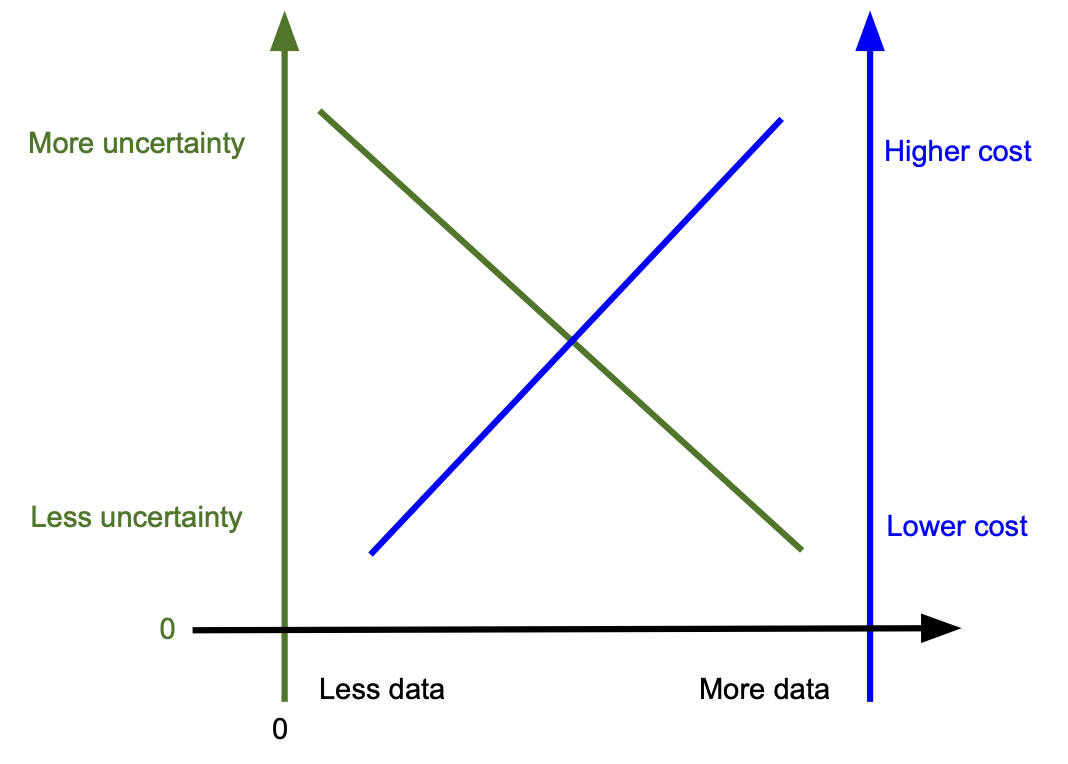
\includegraphics[width=0.8\textwidth]{images/cost_and_uncertainty_for_data_collection}
        \caption{Collecting more data costs money and time and decreases uncertainty.  See Dilemma~\ref{table:dilemma-personal-gather-data-lots-vs-little}. This plot is wrong for multiple reasons. Cost, whether temporal or financial, does not increase linearly with data quantity. Similarly uncertainty is not linear with data quantity. Even quantifying uncertainty is challenging. }
        \label{fig:data_collection_cost_uncertainty}
\end{figure}



% explanation of context for dilemma
% How does this relate directly to bureaucracy as defined as shared resource management policymaking?
Decision making is foundational to bureaucracy, so gathering data to inform decisions is crucial. There's typically insufficient time and resources available for this work, which results in imperfect decisions. 

The \hyperref[table:dilemma-personal-gather-data-lots-vs-little]{Dilemma of Data Quantity} is more nuanced than merely finding 
\href{https://en.wikipedia.org/wiki/Goldilocks_principle}{just the right amount} of data.
\index{Wikipedia!\href{https://en.wikipedia.org/wiki/Goldilocks_principle}{Goldilocks principle}}
\marginpar{[Wikipedia] Goldilocks principle}
The skill is knowing which data is most relevant to the decision, and having relationships with data owners to ease the cost of gathering data.

% How does this effect your relationships with other bureaucrats?
The logistics of gathering data can be measured, but there are other subjective aspects to account for as well. Making a decision has an emotional toll on the decider due to the risk of failure. Also, decisions are made in a social context, with decision makers accounting for the ramifications on people they have relationships with. 
%The \hyperref[table:dilemma-personal-gather-data-lots-vs-little]{Dilemma of Data Quantity}

% Are the incentive structures aligned to support one direction or the other?
While gathering less data means less cost for the bureaucrat facing a decision, you might imagine some accountability for bad decisions due to inadequate data. To shield individual bureaucrats from reputation-harming liability, a decision may require an approval chain. That review process diffuses responsibility for decisions.


The \hyperref[table:dilemma-personal-gather-data-lots-vs-little]{Dilemma of Gathering data} is distinct from the \hyperref[table:dilemma-personal-planning-vs-iterate]{Dilemma of Planning}. It is possible to do a lot of planning with only a little information gathered, and it is feasible to have lots of data and do no planning. 

\begin{center}
\begin{table}[H] % ht
\begin{tabular}{ | m{\dilemmatablewidth}| m{\dilemmatablewidth} | } 
  \hline
  \textbf{Extensive planning upfront (proactive).} & 
  \textbf{Iterative improvement of plans (reactive).} \\ 
  \hline
  \textit{Description}: Lots of time spent brainstorming potential scenarios and contingency options prior to taking action. & 
  \textit{Description}: Start taking action and use feedback to shape next actions. \\ 
  \hline
  \textit{Cons}: ``No plan survives contact with the enemy.'' {\small -\href{https://en.wikipedia.org/wiki/Helmuth_von_Moltke_the_Elder}{von Moltke}
  \index{Wikipedia!\href{https://en.wikipedia.org/wiki/Helmuth_von_Moltke_the_Elder}{Helmuth von Moltke}}
  } & 
  % initially the citation to Wiki page was a footnote, but footnote doesn't work inside a table
  % second approach was to use \footnotemark and \footnotetext[1]{link} as per https://tex.stackexchange.com/a/109470/235813 but the footnote ended up on the next page with the wrong index
  \textit{Cons}: Less prepared. \\  
  \hline
\end{tabular}
\caption{
\textit{Dilemma of Planning.}
\index{dilemma!of planning}
How much time to invest in different types of planning.
%{\tiny Tag: Decision making.}
}
\label{table:dilemma-personal-planning-vs-iterate}
%GV     "dilemma-personal-planning-vs-iterate" [label="how much planning", shape="box"];
%GV     "dilemma-personal-planning-vs-iterate" -> "plan";
%GV     "dilemma-personal-planning-vs-iterate" -> "iterate";
\end{table}
\end{center}

% explanation of context for dilemma
Managing a shared resource requires more than just on-the-spot decision making. Thinking ahead to potential scenarios that effect the shared resource is the responsibility of the bureaucrat. 

% How does this relate directly to bureaucracy as defined as shared resource management policymaking?
The \hyperref[table:dilemma-personal-planning-vs-iterate]{Dilemma of Planning} identifies a widely applicable challenge for bureaucrats throughout an organization (top to bottom, and on every team). Regardless of whether you're planning your next day or the next few years, there will be unforeseen challenges. Do those interruptions invalidate the effort of planning?

% How does this effect your relationships with other bureaucrats?
The \hyperref[table:dilemma-personal-planning-vs-iterate]{Dilemma of Planning} induces different responses for each bureaucrat, so you will likely encounter both someone who you think plans too much and someone who doesn't plan enough. Being exclusively reactionary can be demoralizing, as can seeing your plans become moot.

% Are the incentive structures aligned to support one direction or the other?



Making a decision imposes a bound on how much time is available for both gathering data and planning. More time gathering data is less time planning. Similarly, the number of people available for data gathering and planning is bounded, and tasking people is a zero sum choice.

\begin{figure}[H] % ht
    \centering
    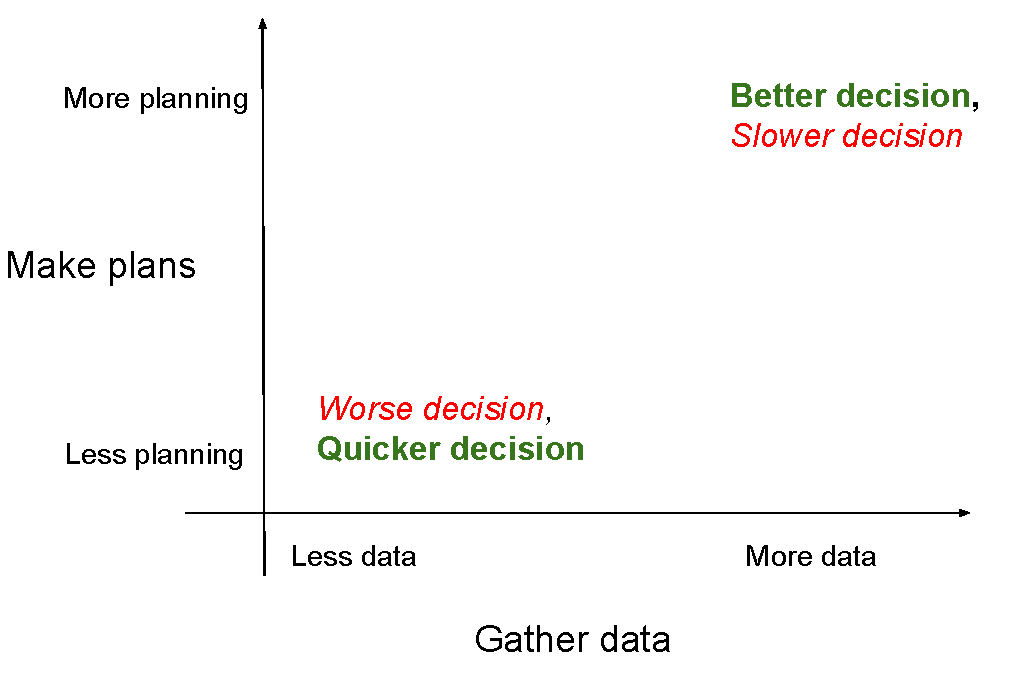
\includegraphics[width=0.8\textwidth]{images/planning_and_data_gathering.pdf}
    \caption{Planning (Dilemma~\ref{table:dilemma-personal-planning-vs-iterate}) and data gathering (Dilemma~\ref{table:dilemma-personal-gather-data-lots-vs-little}) trade-off.}
    \label{fig:pareto_frontier}
\end{figure}

%In practice, gathering data and planning rarely terminate -- they evolve.



When planning (Dilemma~\ref{table:dilemma-personal-planning-vs-iterate}), aspects to consider include
%\begin{itemize}
%    \item 
the amount of risk seeking or risk tolerance (Dilemma~\ref{table:dilemma-personal-risk-high-vs-low})
and
%    \item 
the intended scope of effect  (Dilemma~\ref{table:dilemma-personal-scope-broad-vs-narrow}).
%\end{itemize}

\begin{center}
\begin{table}[H] % ht
\begin{tabular}{ | m{\dilemmatablewidth}| m{\dilemmatablewidth} | } 
  \hline
  \textbf{Take on big risks and big rewards.} & 
  \textbf{Take on small risks and small rewards.} \\ 
  \hline
  \textit{Description}: High risk tolerance. &
  \textit{Description}: Low risk tolerance. \\
  \hline
  \textit{Pros}: Potential for failure and harm is significant. &
  \textit{Pros}: If any one investment fails, you can continue other efforts. \\
  \hline
  \textit{Cons}: Costly investment, longer feedback cycle. & 
  \textit{Cons}: Incremental can be slower. \\
  \hline
\end{tabular}
\caption{
\textit{Dilemma of \href{https://en.wikipedia.org/wiki/Risk_assessment}{Risk tolerance}.
\index{Wikipedia!\href{https://en.wikipedia.org/wiki/Risk_assessment}{Risk tolerance}}
} 
\index{dilemma!of \href{https://en.wikipedia.org/wiki/Risk_assessment}{Risk tolerance}}
%{\tiny Tag: Personal choice.}
}
\label{table:dilemma-personal-risk-high-vs-low}
%GV     "dilemma-personal-risk-high-vs-low" [label="big risk or small risk", shape="box"];
%GV     "dilemma-personal-risk-high-vs-low" -> "risk";
\end{table}
\end{center}

% explanation of context for dilemma
Taking big leaps can be exciting. But you might be leaping to failure. Small leaps are less risky, supporting an evolutionary path to discovery. 

% How does this relate directly to bureaucracy as defined as shared resource management policymaking?
The \hyperref[table:dilemma-personal-risk-high-vs-low]{Dilemma of Risk Tolerance} arises in bureaucracy because the environment around the shared resource being managed isn't static. Change requires policies and processes to change. Whether the change is small or large is dependent on the risk tolerance of individual bureaucrats involved in the decision. 

% How does this effect your relationships with other bureaucrats?
The risk tolerance of individuals is shaped by their experience. What you see as conventional and routine another bureaucrat would regard as untested. 

%The \hyperref[table:dilemma-personal-risk-high-vs-low]{Dilemma of Risk Tolerance}
% Are the incentive structures aligned to support one direction or the other?
The bias for bureaucrats is towards smaller risks. That way if failure does occur the bureaucrat incurs less harm to their reputation. As a consequence, significant 
\hyperref[sec:innovation]{innovation} is difficult in bureaucratic organizations. 


\begin{center}
\begin{table}[H]
\begin{tabular}{ | m{\dilemmatablewidth}| m{\dilemmatablewidth} | } 
  \hline
  \textbf{Involve people who disagree.} & 
  \textbf{Ignore people who disagree.} \\ 
  \hline
  \textit{Pros}: Get constructive feedback; account for factors you didn't consider; build a robust solution. & 
  \textit{Pros}: Save time by not interacting. \\  
  \hline
  \textit{Cons}: Results in a compromise or partial solution that minimizes aggregate unhappiness. & 
  \textit{Cons}: Miss a vital aspect you didn't consider. \\  
  \hline
\end{tabular}
\caption{\textit{Dilemma of Disagreement.}
\index{dilemma!of disagreement}
Engagement with opposition to process or change.
%{\tiny Tag: Decision making.}
}
\label{table:dilemma-personal-opposition-involve-ignore}
%GV     "dilemma-personal-opposition-involve-ignore" [label="involve opposition or ignore", shape="box"];
%GV     "dilemma-personal-opposition-involve-ignore" -> "disagree";
\end{table}
\end{center}

%  explanation of context for dilemma


% How does this relate directly to bureaucracy as defined as shared resource management policymaking?
Bureaucracy is the subjective decision making associated with management of shared resource, so the existence of people who disagree is not surprising. The choice you face is whether to engage with people who think you're wrong. 

% How does this effect your relationships with other bureaucrats?
The \hyperref[table:dilemma-personal-opposition-involve-ignore]{Dilemma of Disagreement} is sensitive to how social you are and how well you can negotiate. If you can hear criticism of your idea and not take it personally, you are more capable of getting constructive feedback. Having relationships where that level of honesty is available is a long-term investment.

%
% Are the incentive structures aligned to support one direction or the other?
The default behavior for bureaucrats facing the \hyperref[table:dilemma-personal-opposition-involve-ignore]{Dilemma of Disagreement} is to avoid negative input. What you might consider innovation another person might see as wasteful. To avoid that risk, don't share what you're working on.

\begin{center}
\begin{table}[H] % ht
\begin{tabular}{ | m{\dilemmatablewidth}| m{\dilemmatablewidth} | } 
  \hline
  \textbf{Broad scope of effect.} &
  \textbf{Narrow scope of effect.} \\
  \hline
  \textit{Description}: The consequence of the work has many stakeholders. &
  \textit{Description}: Small number of stakeholders. \\  
  \hline
  \textit{Pros}: Benefit more people. &
  \textit{Pros}: Niche effect means less dependencies on other people. \\
  \hline
  \textit{Cons}: Harder to get everyone in agreement. & 
  \textit{Cons}: Less visibility to the rest of the organization. \\
  \hline
\end{tabular}
\caption{
\textit{Dilemma of Scope of Effect.}
\index{dilemma!of scope of effect}
Scope of effect of your work. 
%{\tiny Tag: Personal choice}
}
\label{table:dilemma-personal-scope-broad-vs-narrow}
%GV     "dilemma-scope-broad-vs-narrow" [label="scope of effect broad vs narrow", shape="box"];
%GV     "dilemma-scope-broad-vs-narrow" -> "scope";
\end{table}
\end{center}

% explanation of context for dilemma
Framed as ``should you work on something consequential?" the naive answer is to say yes. However, to make effective change involves coordinating more stakeholders than you may be comfortable with. Experienced bureaucrats are more likely to crave off a small portion of a big challenge.

% How does this relate directly to bureaucracy as defined as shared resource management policymaking?
You may have some freedom to choose what you work on, in which case the \hyperref[table:dilemma-personal-scope-broad-vs-narrow]{Dilemma of Scope of Effect} is in play. Mentorship from more experienced bureaucrats can help you decide what scope of task is big enough to be meaningful but not too big as to be intractable.

% How does this effect your relationships with other bureaucrats?
%The \hyperref[table:dilemma-personal-scope-broad-vs-narrow]{Dilemma of Scope of Effect}
% Are the incentive structures aligned to support one direction or the other?


\ \\

Once \hyperref[table:dilemma-personal-gather-data-lots-vs-little]{data is gathered} (Dilemma~\ref{table:dilemma-personal-gather-data-lots-vs-little}) and a \hyperref[table:dilemma-personal-planning-vs-iterate]{plan is made} (Dilemma~\ref{table:dilemma-personal-planning-vs-iterate}), the result is disseminated. The choices of how to disseminate are the \hyperref[table:dilemma-personal-consistency-gradual-stepwise]{Dilemma of Consistency over time} (\ref{table:dilemma-personal-consistency-gradual-stepwise}) and the \hyperref[table:dilemma-personal-disseminate-one-by-one]{Dilemma of Disseminating information} (\ref{table:dilemma-personal-disseminate-one-by-one}).

\begin{center}
\begin{table}[H] % ht
\begin{tabular}{ | m{\dilemmatablewidth}| m{\dilemmatablewidth} | } 
  \hline
  \textbf{Guidance updated often; incremental change.} & 
  \textbf{Consistent application of policy over time. Rules persist; then sudden drastic change.} \\ 
  \hline
  \textit{Pros}: Adapt policy to new information and changing conditions. &
  \textit{Pros}: Stability is easier to predict between regime changes.  \\
  \hline
  \textit{Cons}: More work needed for revisions. Accused of lacking stability. & 
  \textit{Cons}: Doesn't adapt as conditions change. Accused of being inflexible to evolving conditions. \\
  \hline
\end{tabular}
\caption{
\textit{Dilemma of Consistency over time.} 
\index{dilemma!of consistency over time}
Stability of rules; how change is enacted. Can also be characterized as when to tell other people: sooner (decreases surprise) or later (when firmer information is available).
See the description of 
\hyperref[sec:static-dynamic-processes]{static versus dynamic processes} on page~\pageref{sec:static-dynamic-processes}.
%\ifpageref
%on page~\pageref{sec:static-dynamic-processes}
%\fi
%\iftoggle{pageref}{%
%on page~\pageref{sec:static-dynamic-processes}
%}
%\iftoggle{sectionref}{%
%in section~\ref{sec:static-dynamic-processes} 
%}
%{\tiny Tag: Organization's culture. Tag: Personal choice.}
}
\label{table:dilemma-personal-consistency-gradual-stepwise}
%GV     "dilemma-personal-consistency-gradual-stepwise" [label="incremental or step-wise change", shape="box"];
%GV     "dilemma-personal-consistency-gradual-stepwise" -> "consistency";
\end{table}
\end{center}

Deployment of products in industry and deployment of policies in a bureaucracy face similar dilemmas. The \href{https://en.wikipedia.org/wiki/Diffusion_of_innovations}{Diffusion of Innovation} 
\index{Wikipedia!\href{https://en.wikipedia.org/wiki/Diffusion_of_innovations}{Diffusion of Innovation}}
describes how innovation is adopted by people with different amounts of risk tolerance.

% How does this relate directly to bureaucracy as defined as shared resource management policymaking?
Bureaucracy arises to manage shared resources. Management occurs by policies and processes. The community accessing the shared resource changes over time, so the policies and processes evolve to reflect that change. The \hyperref[table:dilemma-personal-consistency-gradual-stepwise]{Dilemma of Consistency over time} is about the degree of incrementalism of the change.

% How does this effect your relationships with other bureaucrats?
Bureaucrats responsible for carrying out policies and processes disagree on the question of stability. This disagreement generates friction for other processes reliant on those relations within an organization.
The \hyperref[table:dilemma-personal-consistency-gradual-stepwise]{Dilemma of Consistency over time} is also disruptive to the subjects of bureaucracy. 

% Are the incentive structures aligned to support one direction or the other?
Bureaucrats are incentivized to avoid change, so the bias in this dilemma is towards consistency and stability even if that means not adapting to current local circumstances. 

\begin{center}
\begin{table}[H] % ht
\begin{tabular}{ | m{\dilemmatablewidth}| m{\dilemmatablewidth} | } 
  \hline
  \textbf{Tell people one-by-one.} & 
  \textbf{Tell everyone at once.} \\ 
  \hline
  \textit{Pros}: One-on-one allows a freer response from audience. &
  \textit{Pros}: Saves time for the speaker. \\
  \hline
  \textit{Cons}: Order matters for relationships. & 
  \textit{Cons}: Overwhelming feedback all at once. Some people don't feel heard. \\  
  \hline
\end{tabular}
\caption{
\textit{Dilemma of Disseminating information.}
\index{dilemma!of disseminating information}
%{\tiny Tag: Personal choice.}
}
\label{table:dilemma-personal-disseminate-one-by-one}
%GV     "dilemma-personal-disseminate-one-by-one" [label="notify one-by-one ar at once", shape="box"];
%GV     "dilemma-personal-disseminate-one-by-one" -> "";
\end{table}
\end{center}

Once a decision has been made, the decision is executed or enforced. \hyperref[table:dilemma-personal-number-of-rules]{How many rules are there} (Dilemma~\ref{table:dilemma-personal-number-of-rules}) and
\hyperref[table:dilemma-personal-rule-strictness-lax]{how strictly are the rules enforced} (Dilemma~\ref{table:dilemma-personal-rule-strictness-lax})?

% How does this relate directly to bureaucracy as defined as shared resource management policymaking?
Bureaucracy involves coordination to facilitate distributed knowledge and distributed decision making. Each bureaucrat has finite time and attention. When communication channels are instantaneous (e.g., phone, email, video) there is often more information to be consumed.
The \hyperref[table:dilemma-personal-disseminate-one-by-one]{Dilemma of Disseminating information} is a question of whether to save time by telling all stakeholders at one time or demonstrate the importance of a relationship by talking one-on-one. 

% How does this effect your relationships with other bureaucrats?

One aspect of the \hyperref[table:dilemma-personal-disseminate-one-by-one]{Dilemma of Disseminating information} can be addressed using personalized emails. Rather than send an email notice to 10 people, automating the process of sending 10 separate emails can make it appear to each recipient that the conversation is one-on-one.  That doesn't resolve the challenge of getting all feedback at once.

% Are the incentive structures aligned to support one direction or the other?
Whether to apply \href{https://en.wikipedia.org/wiki/Nemawashi}{Nemawashi} 
\index{Wikipedia!\href{https://en.wikipedia.org/wiki/Nemawashi}{Nemawashi}}
\marginpar{[Wikipedia] Nemawashi}
or not depends on how much time to allocate to sharing the information. 

\begin{center}
\begin{table}[H] % ht
\begin{tabular}{ | m{\dilemmatablewidth}| m{\dilemmatablewidth} | } 
  \hline
  \textbf{Enforce rules strictly.} & 
  \textbf{Lax rule enforcement.} \\ 
  \hline
  \textit{Pros}: Predictable. &
  \textit{Pros}: Bureaucrats feel empowered. Tolerance for changing conditions or exceptional cases. \\
  \hline
  \textit{Cons}: Insensitive to nuance. & 
  \textit{Cons}: Enforcement is subjective and unpredictable.  \\  
  \hline
\end{tabular}
\caption{
\textit{Dilemma of Strictness of rules.}
\index{dilemma!of strictness of rules}
%{\tiny Tag: Organization's culture.}
}
\label{table:dilemma-personal-rule-strictness-lax}
%GV     "dilemma-personal-rule-strictness-lax" [label="enforce rules strict or lax", shape="box"];
%GV     "dilemma-personal-rule-strictness-lax" -> "rules";
\end{table}
\end{center}

% How does this relate directly to bureaucracy as defined as shared resource management policymaking?
Bureaucracy is the subjective decision making associated with shared resources. Interpretation of rules and enforcement of rules is not objective. Bureaucrats are empowered to make trade-offs specific to the circumstances being considered.

% explanation of context for dilemma

The 
\hyperref[table:dilemma-personal-rule-strictness-lax]{Dilemma of Strictness of rules} 
is about how the bureaucrat enforcing policies decides to act, whereas the
\hyperref[table:dilemma-subject-consistency-per-situation]{Dilemma of Consistency} 
(whether to seek exceptions) and
\hyperref[table:dilemma-subject-flexibility]{Dilemma of Flexible Rules}
are from the subjects view. While the objective question is similar, the rationalization for behavior depends on which role is being considered.

Bureaucrats and subjects of bureaucracy both complain regardless of where on the spectrum each instances of \hyperref[table:dilemma-personal-rule-strictness-lax]{Dilemma of Strictness of rules} occurs. 

% How does this effect your relationships with other bureaucrats?
Different bureaucrats will evaluate which rules apply in each circumstance slightly differently. Barring consensus, the organization's hierarchy is used to have one person decide what the relevant interpretation is.

% Are the incentive structures aligned to support one direction or the other?
The default behavior is strict enforcement since that is a defensible story for the responsible bureaucrat. Exceptions based on personal relationships do not appear fair to outsiders.


\begin{center}
\begin{table}[H] % ht
\begin{tabular}{ | m{\dilemmatablewidth}| m{\dilemmatablewidth} | } 
  \hline
  \textbf{Control via rules.} & 
  \textbf{Freedom/autonomy/agility.} \\ 
  \hline
  \textit{Description}: High number of rules to cover various situations. & 
  \textit{Description}: Low number of rules to enable flexibility. \\ 
  \hline
  \textit{Cons}: The more rules that exist the more likely it is that someone will find a way to exploit them to their own advantage. & 
  \textit{Cons}: The fewer rules that exist the more likely it is that someone will try to get away with something bad. \\  
  \hline
\end{tabular}
\caption{
\textit{Dilemma of Number of rules.}
\index{dilemma!of number of rules}
%{\tiny Tag: Organization's culture}
}
\label{table:dilemma-personal-number-of-rules}
%GV     "dilemma-personal-number-of-rules" [label="rule or freedom", shape="box"];
%GV     "dilemma-personal-number-of-rules" -> "rules";
\end{table}
\end{center}



%  explanation of context for dilemma
% How does this relate directly to bureaucracy as defined as shared resource management policymaking?
The \hyperref[table:dilemma-personal-number-of-rules]{Dilemma of Number of rules}
\marginpar{[Tag] \href{https://en.wikipedia.org/wiki/Goldilocks_principle}{Goldilocks balance}}
\index{Goldilocks balance!number of rules}
arises in bureaucratic organizations because bureaucrats have to make subjective decisions about shared resources. 

% How does this effect your relationships with other bureaucrats?
%The \hyperref[table:dilemma-personal-number-of-rules]{Dilemma of Number of rules}
% Are the incentive structures aligned to support one direction or the other?

An alternative approach to the  \hyperref[table:dilemma-personal-number-of-rules]{Dilemma of Number of rules}
is to use guidance derived from principles. A principles-based approach relies on good judgment which can be adapted to specific situations. What qualifies as ``good'' has subjective boundary conditions and requires knowledge of the situation.



\begin{center}
\begin{table}[H] % ht
\begin{tabular}{ | m{\dilemmatablewidth}| m{\dilemmatablewidth} | } 
  \hline
  \textbf{If it's not against the rules, it must be okay.} & 
  \textbf{I can only do what is allowed by the rules and nothing more.} \\ 
  \hline
  \textit{Description}: I can do anything that's not illegal. &
  \textit{Description}: Do only what is mandated by the organization. \\
  \hline
  \textit{Pros}: Autonomy, flexibility. &
  \textit{Pros}: Less risk of getting in trouble. \\
  \hline
  \textit{Cons}: What one person deems reasonable another may not. & 
  \textit{Cons}: Constrains creative solutions. Less productive. Responding to novel situations is inhibited. \\  
  \hline
\end{tabular}
\caption{
\textit{Dilemma of Adherence to rules} depends on an individual's risk tolerance versus aversion to risk. 
The scope of your actions bound by mandates and legality, but the way you interpret that is subjective. 
Constraining activities to explicitly specified rules can be used as an excuse for laziness. 
\index{dilemma!of adherence to rules}
}
\label{table:dilemma-personal-rule-adherence}
%GV     "dilemma-personal-rule-adherence" [label="rules allow or conform", shape="box"];
%GV     "dilemma-personal-rule-adherence" -> "rules";
\end{table}
\end{center}

%  explanation of context for dilemma
Your understanding of your freedom versus responsibilities may be a philosophical topic, but it can manifest in bureaucratic organizations. Being a member of an organization means leveraging the resources available or acting in accordance with mandates. 

% How does this relate directly to bureaucracy as defined as shared resource management policymaking?

The \hyperref[table:dilemma-personal-rule-adherence]{Dilemma of Adherence to rules}
\footnote{See \href{https://en.wikipedia.org/wiki/Everything_which_is_not_forbidden_is_allowed}{Everything which is not forbidden is allowed} 
\index{Wikipedia!\href{https://en.wikipedia.org/wiki/Everything_which_is_not_forbidden_is_allowed}{Everything which is not forbidden is allowed}}
on Wikipedia.} is used by bureaucrats to rationalize their action (or inaction). 

% How does this effect your relationships with other bureaucrats?
Changing a coworker's attitude on this topic if they disagree with your understanding can rely on appeals to authority or emotional reassurance, depending on their stance.

%The \hyperref[table:dilemma-personal-rule-adherence]{Dilemma of Adherence to rules}
% Are the incentive structures aligned to support one direction or the other?

\begin{center}
\begin{table}[H] % ht
\begin{tabular}{ | m{\dilemmatablewidth}| m{\dilemmatablewidth} | } 
  \hline
  \textbf{A decision in a process is informed by a single bit of information.} & 
  \textbf{Fault tolerant decision making through redundancy.} \\ 
  \hline
  \textit{Description}: A form featuring a checkbox option. & 
  \textit{Description}: Multiple independent confirmations that the data collected is correct.  \\
  \hline
  \textit{Pros}: Less overhead. & 
  \textit{Pros}: Decrease mistakes. \\
  \hline
  \textit{Cons}: Single point of failure. Might be accidentally wrong. &
  \textit{Cons}: More time needed. Extra burden of collecting and processing more data. \\  
  \hline
\end{tabular}
\caption{
\textit{Dilemma of Redundant Data for Decisions.}
\index{dilemma!of redundant data for decisions}
Having a single checkbox on a form makes data collection easier for both the subject and the bureaucrat. However, the person using the form might not see the checkbox or may accidentally fill in the checkbox. Is there any validation of the selection? The process is sensitive to this single bit of data. This applies to written forms and verbal conversations. 
}
\label{table:dilemma-personal-single-bit-decision}
%GV     "dilemma-personal-single-bit-decision" [label="single bit error", shape="box"];
%GV     "dilemma-personal-single-bit-decision" -> "redundancy";
\end{table}
\end{center}

%  explanation of context for dilemma
With the intent of streamlining interactions between subjects and bureaucrats, collecting as little data as is needed benefits both parties. Bureaucratic management of shared resources depends on decision making, and decisions require information. 


% How does this relate directly to bureaucracy as defined as shared resource management policymaking?
The \hyperref[table:dilemma-personal-gather-data-lots-vs-little]{Dilemma of Data Quantity} is about how much data is needed, whereas the \hyperref[table:dilemma-personal-single-bit-decision]{Dilemma of Redundant Data for Decisions} is about the redundancy of data used for coordination. While not unique to bureaucracy, the lack of feedback loops motivating correct information can lead to harm for participants.

% How does this effect your relationships with other bureaucrats?
Most decisions are of low importance, so the correctness of information is rarely checked. Redundant information is deemed wasteful, and those habits don't necessarily change when the significance of a decision increases. 

The \hyperref[table:dilemma-personal-single-bit-decision]{Dilemma of Redundant Data for Decisions} presents a lose-lose situation: collect redundant information (which introduces additional risk of conflicting information) or hope that data collected represents reality without checking. 

% Are the incentive structures aligned to support one direction or the other?

\begin{center}
\begin{table}[H] % ht
\begin{tabular}{ | m{\dilemmatablewidth}| m{\dilemmatablewidth} | } 
  \hline
  \textbf{A single bureaucrat reviews information and makes a decision.} & 
  \textbf{Fault tolerant decision making using multiple reviewers.} \\ 
  \hline
  \textit{Description}: A decision process relies on a single bureaucrat. & 
  \textit{Description}: Multiple independent confirmations of a decision.  \\
  \hline
  \textit{Pros}: Less overhead. & 
  \textit{Pros}: Decrease mistakes. \\
  \hline
  \textit{Cons}: Single point of failure. Might get policy interpretation wrong. &
  \textit{Cons}: More time and staffing needed. Less ownership of decisions. \\  
  \hline
\end{tabular}
\caption{
\textit{Dilemma of Redundant Reviewers.}
\index{dilemma!of redundant reviewers}
Having a single bureaucrat make a decision is quicker than checking that person, but validating the decision slows down the process and requires additional bureaucrats getting involved.
}
\label{table:dilemma-personal-redundant-reviewers}
%GV     "dilemma-personal-redundant-reviewers" [label="redundant reviewers", shape="box"];
%GV     "dilemma-personal-redundant-reviewers" -> "redundancy";
\end{table}
\end{center}

% TODO: Explanation of context for dilemma
% How does this relate directly to bureaucracy as defined as shared resource management policymaking?
%The \hyperref[table:]{Dilemma of }
% How does this effect your relationships with other bureaucrats?
%The \hyperref[table:]{Dilemma of }
% Are the incentive structures aligned to support one direction or the other?

\begin{center}
\begin{table}[H] % ht
\begin{tabular}{ | m{\dilemmatablewidth}| m{\dilemmatablewidth} | } 
  \hline
  \textbf{Quickly complete tasks or deploy new policies or create new products.} & 
  \textbf{Methodically complete tasks (or well-founded policies, quality products).} \\ 
  \hline
  \textit{Description}: Enact a solution quickly to address urgent needs. &
  \textit{Description}: Methodical well-planned design and execution yield robust solutions/products/policies. \\
  \hline
  \textit{Pros}: Rapid solution. &
  \textit{Pros}: More like to get the solution right. \\
  \hline
  \textit{Cons}: Risk of quick task is that the result is ineffective, inefficient, or wrong. &
  \textit{Cons}: \href{https://en.wikipedia.org/wiki/Opportunity_cost}{opportunity cost}. 
  \index{Wikipedia!\href{https://en.wikipedia.org/wiki/Opportunity_cost}{opportunity cost}}
  \\  
  \hline
\end{tabular}
\caption{
\textit{Dilemma of Speed and Accuracy.}
\index{dilemma!of speed and accuracy}
Speed versus accuracy of task completion.
}
\label{table:dilemma-personal-quick-methodical}
%GV     "dilemma-personal-quick-methodical" [label="quick or methodical", shape="box"];
%GV     "dilemma-personal-quick-methodical" -> "speed";
\end{table}
\end{center}

If you try to resolve the \hyperref[table:dilemma-personal-quick-methodical]{Dilemma of Speed and Accuracy} by both getting a solution deployed quickly and then iterating towards a robust outcome, you may appear unpredictable or unstable; see Dilemma~\ref{table:dilemma-personal-planning-vs-iterate}. This is an example of cascading dilemmas. The interplay of a creative resolution to one dilemma can effect the solution space for other dilemmas. 

%  explanation of context for dilemma
% How does this relate directly to bureaucracy as defined as shared resource management policymaking?
%The \hyperref[table:dilemma-personal-quick-methodical]{Dilemma of Speed and Accuracy}
% How does this effect your relationships with other bureaucrats?
Regardless of where on this spectrum you are with the \hyperref[table:dilemma-personal-quick-methodical]{Dilemma of Speed and Accuracy}, someone that you depend on in the bureaucracy will take the opposite stance. This becomes a source of friction regarding how long tasks should take. 

% Are the incentive structures aligned to support one direction or the other?
The bias for this dilemma is that most bureaucrats want to be perceived as methodical and careful. Quick judgment is seen as risky. 


\begin{center}
\begin{table}[H] % ht
\begin{tabular}{ | m{\dilemmatablewidth}| m{\dilemmatablewidth} | } 
  \hline
  \textbf{Push people to work really hard.} & 
  \textbf{Create a comfortable work environment.} \\ 
  \hline
  \textit{Cons}: Burn out and leave. & 
  \textit{Cons}: Lower instantaneous productivity. \\  
  \hline
\end{tabular}
\caption{
\textit{Dilemma of Urgency.}
\index{dilemma!of urgency}
}
\label{table:dilemma-personal-manager-rate-of-work}
%GV     "dilemma-personal-manager-rate-of-work" [label="work hard or sustainably", shape="trapezium"];
%GV     "dilemma-personal-manager-rate-of-work" -> "level-of-effort";
%GV     "dilemma-personal-manager-rate-of-work" -> "dilemma-personal-work-extra-or-work-as-expected" [dir=none];
\end{table}
\end{center}

% How does this relate directly to bureaucracy as defined as shared resource management policymaking?
There is usually a large range of productivity possible for a bureaucrat. Management has input on what is expected from bureaucrat. The 
\hyperref[table:dilemma-personal-manager-rate-of-work]{Dilemma of Urgency} reflects the trade-off of how much to push employees of an organization. The \hyperref[table:dilemma-personal-manager-rate-of-work]{Dilemma of Urgency} is the manager's perspective, whereas the
\hyperref[table:dilemma-personal-work-extra-or-work-as-expected]{Dilemma of Working extra hard}
is the view of the bureaucrat. 

% How does this effect your relationships with other bureaucrats?
%The \hyperref[table:dilemma-personal-manager-rate-of-work]{Dilemma of Urgency}

% Are the incentive structures aligned to support one direction or the other?
Because of weak feedback loops in bureaucratic organizations, bureaucrats default to a relaxed work environment. Examples of exceptions to this include seasonal variations like tax collection time for the \href{https://en.wikipedia.org/wiki/Internal_Revenue_Service}{IRS} 
\index{Wikipedia!\href{https://en.wikipedia.org/wiki/Internal_Revenue_Service}{Internal Revenue Service}}
\index{exemplar!\href{https://en.wikipedia.org/wiki/Internal_Revenue_Service}{Internal Revenue Service (IRS)}}
and demand spikes like a natural disaster for \href{https://en.wikipedia.org/wiki/Federal_Emergency_Management_Agency}{FEMA}. 
\index{Wikipedia!\href{https://en.wikipedia.org/wiki/Federal_Emergency_Management_Agency}{Federal Emergency Management Agency}}
\index{exemplar!\href{https://en.wikipedia.org/wiki/Federal_Emergency_Management_Agency}{Federal Emergency Management Agency (FEMA)}}

% https://bennorthrop.com/Essays/2022/code-ownership-stewardship-or-free-for-all.php
\begin{center}
\begin{table}[H] % ht
\begin{tabular}{ | m{\dilemmatablewidth}| m{\dilemmatablewidth} | } 
  \hline
  \textbf{Talk more to convey more information.} & 
  \textbf{Listen more to learn more information.} \\ 
  \hline
  \textit{Cons}: Less time available for listening. & 
  \textit{Cons}: Less time to convey what you know. \\  
  \hline
\end{tabular}
\caption{
\textit{Dilemma of Talking.}
\index{dilemma!of talking}
In conversations or meetings there is a (subjective) balance for participants.
}
\label{table:dilemma-personal-talk-or-listen}
%GV     "dilemma-personal-talk-or-listen" [label="talk or listen", shape="box"];
%GV     "dilemma-personal-talk-or-listen" -> "speak";
\end{table}
\end{center}

% How does this relate directly to bureaucracy as defined as shared resource management policymaking?
The \hyperref[table:dilemma-personal-talk-or-listen]{Dilemma of Talking} captures the zero-some information constraint that most bureaucrats can't concurrently talk and listen. 

% How does this effect your relationships with other bureaucrats?
The \hyperref[table:dilemma-personal-talk-or-listen]{Dilemma of Talking} depends on the personality of each bureaucrat involved in coordination of distributed knowledge and distributed decision making. Some are patient listeners, while others feel uncomfortable with silence.

% Are the incentive structures aligned to support one direction or the other?
Talking constructively about work takes effort, so the default here is to not communicate. 


\begin{center}
\begin{table}[H] % ht
\begin{tabular}{ | m{\dilemmatablewidth}| m{\dilemmatablewidth} | } 
  \hline
  \textbf{Seek out experienced collaborators.} & 
  \textbf{Work with less experienced people.} \\ 
  \hline
  \textit{Pros}: Quicker to get something done. &
  \textit{Pros}: Less set in their ways and open to more novelty. \\  
  \hline
  \textit{Cons}: Experienced people who are good are probably busy. &
  \textit{Cons}: Slower progress; more education needed. \\  
  \hline
\end{tabular}
\caption{
\textit{Dilemma of Experienced Collaborators.}
\index{dilemma!of experienced collaborators}
People with experience are useful but less accessible.
}
\label{table:dilemma-personal-experienced-collaborators}
%GV     "dilemma-personal-experienced-collaborators" [label="experienced collaborators or not", shape="box"];
%GV     "dilemma-personal-experienced-collaborators" -> "";
\end{table}
\end{center}


% How does this relate directly to bureaucracy as defined as shared resource management policymaking?
Distributed knowledge in a bureaucracy relies on collaboration among bureaucrats. 
The \hyperref[table:dilemma-personal-experienced-collaborators]{Dilemma of Experienced Collaborators} is about the options of who to collaborate with. 

% How does this effect your relationships with other bureaucrats?

% Are the incentive structures aligned to support one direction or the other?
The bias for the \hyperref[table:dilemma-personal-experienced-collaborators]{Dilemma of Experienced Collaborators} depends on the promotion structure of your organization and the composition of the workforce. If training new member of the team is rewarded, then you might choose to work with less experienced bureaucrats. If the entire team is experienced, then this Dilemma doesn't apply.

\begin{center}
\begin{table}[H] % ht
\begin{tabular}{ | m{\dilemmatablewidth}| m{\dilemmatablewidth} | } 
  \hline
  \textbf{Say yes to new opportunities.} & 
  \textbf{Say no to new opportunities.} \\ 
  \hline
  \textit{Pros}: Positive attitude, collaborative. &
  \textit{Pros}: Able to prioritize and focus. \\
  \hline
  \textit{Cons}: Fail to complete tasks. &
  \textit{Cons}: Not a team player. \\  
  \hline
\end{tabular}
\caption{
\textit{Dilemma of opportunities.}
\index{dilemma!of opportunities}
Acceptance or rejection of more work can be explicit or implicit. Bureaucrats respond to this challenge by sending mixed signals: expressing interest but not following up with action.
}
\label{table:dilemma-new-opportunties-yes-no}
%GV     "dilemma-new-opportunties-yes-no" [label="new opportunities yes or no", shape="box"];
%GV     "dilemma-new-opportunties-yes-no" -> "";
\end{table}
\end{center}

% How does this relate directly to bureaucracy as defined as shared resource management policymaking?
The \hyperref[table:dilemma-new-opportunties-yes-no]{Dilemma of opportunities} depends as much on the workload as on your personality. 

% How does this effect your relationships with other bureaucrats?
Finding ways to avoid doing work while helping the person providing the opportunity is the central skill for the \hyperref[table:dilemma-new-opportunties-yes-no]{Dilemma of opportunities}. This may mean referring the opportunity to another coworker or expressing support but not investing effort. 

% Are the incentive structures aligned to support one direction or the other?


\begin{center}
\begin{table}[H] % ht
\begin{tabular}{ | m{\dilemmatablewidth}| m{\dilemmatablewidth} | } 
  \hline
  \textbf{Share less data.} &
  \textbf{Share more data.} \\
%  \hline
%  \textit{Description}:  &
%  \textit{Description}:  \\  
  \hline
  \textit{Pros}: Restricting data access saves money and time for the data owner.&
  \textit{Pros}: Sharing data improves transparency and accountability. \\
  \hline
  \textit{Cons}: People other than the data owner are unable to extract value from data. & 
  \textit{Cons}: Sharing data uses resources (people, money, time). \\
  \hline
\end{tabular}
\caption{
\textit{Dilemma of Sharing Data.}
\index{dilemma!of sharing data}
How much data to share. Potential solution is to make data discoverable. Advertise the availability of data without providing data. This way a negotiation is feasible for people interested in the data.
%{\tiny Tag: Personal choice.}
}
\label{table:dilemma-data-share-vs-hide}
%GV     "dilemma-data-share-vs-hide" [label="share data less or more", shape="box"];
%GV     "dilemma-data-share-vs-hide" -> "share";
%GV     "dilemma-data-share-vs-hide" -> "data";
\end{table}
\end{center}

In the \hyperref[table:dilemma-data-share-vs-hide]{Dilemma of Sharing Data} there many of aspects of data than can be shared to improve discoverability: who to contact about access, what the data sources are, how often data is collected, how long data is stored, how much data there is.

% How does this relate directly to bureaucracy as defined as shared resource management policymaking?
Distributed knowledge and distributed decision making both rely on having data. Without data the policies and processes of bureaucracy are less effective. 

% How does this effect your relationships with other bureaucrats?
Sharing data is typically perceived as helpful. 
The \hyperref[table:dilemma-data-share-vs-hide]{Dilemma of Sharing Data} points out that the helpfulness has a cost. 

% Are the incentive structures aligned to support one direction or the other?
Because sharing data consumes resources, the bias is to not provide data. That applies to sharing with other bureaucrats within the organization as well as subjects of the bureaucracy. 


\begin{center}
\begin{table}[H] % ht
\begin{tabular}{ | m{\dilemmatablewidth}| m{\dilemmatablewidth} | } 
  \hline
  \textbf{Compete for resources.} &
  \textbf{Cooperate for productivity.} \\
  \hline
  \textit{Description}: individuals compete for attention and promotion; teams compete for money and staffing resources. &
  \textit{Description}: cooperation improves productivity. \\  
  \hline
  \textit{Cons}: Fail to synergize skills resources. & 
  \textit{Cons}: Not clear who to assign responsibility for success or failure. \\
  \hline
\end{tabular}
\caption{
\textit{Dilemma of Cooperate or Compete.} 
\index{dilemma!of cooperate or compete}
Applies to teams and to individuals. 
%{\tiny Tag: Personal choice.}
}
\label{table:dilemma-personal-cooperate-vs-compete}
%GV     "dilemma-personal-cooperate-vs-compete" [label="cooperate or compete", shape="box"];
%GV     "dilemma-personal-cooperate-vs-compete" -> "";
\end{table}
\end{center}

% : explanation of context for dilemma

% How does this relate directly to bureaucracy as defined as shared resource management policymaking?
A bureaucratic organization responsible for management of share resources has finite staffing and money. When there are multiple concurrent efforts relevant to managing the shared resource,  dividing staffing and money is a challenge. 

The \hyperref[table:dilemma-personal-cooperate-vs-compete]{Dilemma of Cooperate or Compete} is best addressed through explicit conversations, both between peers and with decision makers. These discussions may not remedy the challenge, but they provide an opportunity for you to learn more about the people in your organization.

% How does this effect your relationships with other bureaucrats?
The \hyperref[table:dilemma-personal-cooperate-vs-compete]{Dilemma of Cooperate or Compete} can lead to animosity or stronger healthy relationships. 

% Are the incentive structures aligned to support one direction or the other?


\begin{center}
\begin{table}[H] % ht
\begin{tabular}{ | m{\dilemmatablewidth}| m{\dilemmatablewidth} | }
  \hline
  \textbf{Consistent application of policy across cases.} &
  \textbf{Adapt policy to specific cases.} \\
  \hline
  \textit{Description}: Maximize broad applicability; minimize exceptions. &
  \textit{Description}: Demonstrate flexibility for unique scenarios. \\  
  \hline
  \textit{Cons}: Less sensitive to the nuances of a specific situation. & 
  \textit{Cons}: Takes more work. More likely to be accused of bias. \\
  \hline
\end{tabular}
\caption{
\textit{Dilemma of Consistent Policies.}
\index{dilemma!of consistency policies}
Case consistency vs adaptability.
%{\tiny Tag: Personal choice.}
}
\label{table:dilemma-personal-policy-consistency-across-cases}
%GV     "dilemma-personal-policy-consistency-across-cases" [label="consistent policy or adapt", shape="box"];
%GV     "dilemma-personal-policy-consistency-across-cases" -> "consistency";
\end{table}
\end{center}

When change to policies is desired, there are options on how to advocate for change -- Dilemma~\ref{table:dilemma-how-to-change}.

% TODO: explanation of context for dilemma
% How does this relate directly to bureaucracy as defined as shared resource management policymaking?
%The \hyperref[table:policy_consistency_across_cases]{Dilemma of Consistent Policies}
% How does this effect your relationships with other bureaucrats?
%The \hyperref[table:policy_consistency_across_cases]{Dilemma of Consistent Policies}
% Are the incentive structures aligned to support one direction or the other?


% https://bennorthrop.com/Essays/2022/code-ownership-stewardship-or-free-for-all.php
\begin{center}
\begin{table}[H] % ht
\begin{tabular}{ | m{\dilemmatablewidth}| m{\dilemmatablewidth} | } 
  \hline
  \textbf{One person or team owns an area of responsibility.} & 
  \textbf{Anyone take on any task.} \\ 
  \hline
  \textit{Cons}: Staffing capacity may not be as flexible as varying workload. & 
  \textit{Cons}: Not everyone is skilled at everything. \\  
  \hline
\end{tabular}
\caption{
\textit{Dilemma of Swimlanes.} 
\index{dilemma!of swimlanes}
How are tasks assigned? This can be negotiated with coworkers and is not intrinsic to structure of the organization. 
}
\label{table:dilemma-personal-swimlanes}
%GV     "dilemma-personal-swimlanes" [label="swimlanes or not", shape="box"];
%GV     "dilemma-personal-swimlanes" -> "scope";
\end{table}
\end{center}


Independent of how tasks are assigned within a team or organization (Dilemma~\ref{table:dilemma-personal-swimlanes}), individual bureaucrats can decide how they act in Dilemma~\ref{table:dilemma-personal-scope-of-activity}.

% TODO: explanation of context for dilemma
% How does this relate directly to bureaucracy as defined as shared resource management policymaking?
%The \hyperref[table:dilemma-personal-swimlanes]{Dilemma of Swimlanes}
% How does this effect your relationships with other bureaucrats?
%The \hyperref[table:dilemma-personal-swimlanes]{Dilemma of Swimlanes}
% Are the incentive structures aligned to support one direction or the other?


\begin{center}
\begin{table}[H] % ht
\begin{tabular}{ | m{\dilemmatablewidth}| m{\dilemmatablewidth} | }
  \hline
% https://graphthinking.blogspot.com/2019/07/not-too-loose-not-too-tight-determining.html
  \textbf{Adhere strictly to the scope of your role.} & 
  \textbf{Stray outside (or outright ignore) the scope of your role.} \\ 
  \hline
  \textit{Description}: Inflexible to novelty. Specialization of tasking. & 
  \textit{Description}: Lack of structure. Generalization. \\ 
  \hline
  \textit{Cons}: Efficiencies of cooperation and specialization would not occur. Does scale well when flexibility is needed.  & 
  \textit{Cons}: \href{https://en.wikipedia.org/wiki/Deadlock}{Deadlock} 
  \index{Wikipedia!\href{https://en.wikipedia.org/wiki/Deadlock}{Deadlock}}
  condition arises due to a scheduling constraint -- no one can proceed because everyone is waiting on everyone else. Responsibilities are unclear when scope is unclear. \\  
  \hline
\end{tabular}
\caption{
\textit{Dilemma of Scope.}
\index{dilemma!of scope}
Both strict adherence to role scope and ignoring scope can decrease an organization's productivity. 
What happens when a person deviates from their role?
How are people who do not conform identified? Are they confronted?
}
\label{table:dilemma-personal-scope-of-activity}
%GV     "dilemma-personal-scope-of-activity" [label="job scope", shape="box"];
%GV     "dilemma-personal-scope-of-activity" -> "scope";
%GV     "dilemma-personal-scope-of-activity" -> "dilemma-personal-swimlanes" [dir=none];
\end{table}
\end{center}

Best approach to the dilemma of whether to specialize or generalize is to aim to be ``T'' shaped. 

As a specialist, you have two choices: invest in deepening your expertise and skills, or expand the breadth of integration with your team members. Both have the result of improving your organization but they are not equivalent in impact. Educating your coworkers and coordinating actions has a force multiplier effect at burrowing into a problem does not.

% TODO: explanation of context for dilemma
% How does this relate directly to bureaucracy as defined as shared resource management policymaking?
%The \hyperref[table:dilemma-personal-scope-of-activity]{Dilemma of Scope}
% How does this effect your relationships with other bureaucrats?
%The \hyperref[table:dilemma-personal-scope-of-activity]{Dilemma of Scope}
% Are the incentive structures aligned to support one direction or the other?


\begin{center}
\begin{table}[H] % ht
\begin{tabular}{ | m{\dilemmatablewidth}| m{\dilemmatablewidth} | }
  \hline
% https://graphthinking.blogspot.com/2019/07/not-too-loose-not-too-tight-determining.html
  \textbf{Speak outside the scope of your expertise.} & 
  \textbf{Have representative experts participate in discussions.} \\ 
%  \hline
%  \textit{Description}: . & 
%  \textit{Description}: . \\ 
  \hline
  \textit{Pros}: Make progress quickly. & 
  \textit{Pros}: Ensure correct information is shared among stakeholders. \\  
  \hline
  \textit{Cons}: Likely to make mistakes that aren't detected until being enacted. & 
  \textit{Cons}: Getting a diverse group of experts together is logistically challenging since they're busy. \\  
  \hline
\end{tabular}
\caption{
\textit{Dilemma of Speaking Scope.}
\index{dilemma!of speaking scope}
If you don't know what you're talking about, should you speculate or keep your mouth shut?
}
\label{table:dilemma-personal-scope-of-speaking}
%GV     "dilemma-personal-scope-of-speaking" [label="speak outside your expertise", shape="box"];
%GV     "dilemma-personal-scope-of-speaking" -> "scope";
%GV     "dilemma-personal-scope-of-speaking" -> "speak";
\end{table}
\end{center}

Distinguishing speculation from experience is critical in communication. Explaining the basis of your experience is also vital. 

% TODO: explanation of context for dilemma
% How does this relate directly to bureaucracy as defined as shared resource management policymaking?
%The \hyperref[table:dilemma-personal-scope-of-speaking]{Dilemma of Speaking Scope}
% How does this effect your relationships with other bureaucrats?
%The \hyperref[table:dilemma-personal-scope-of-speaking]{Dilemma of Speaking Scope}
% Are the incentive structures aligned to support one direction or the other?

\begin{center}
\begin{table}[H] % ht
\begin{tabular}{ | m{\dilemmatablewidth}| m{\dilemmatablewidth} | }
  \hline
% https://graphthinking.blogspot.com/2019/07/not-too-loose-not-too-tight-determining.html
  \textbf{Have more people participate in a discussion.} & 
  \textbf{Have fewer people participate in a discussion.} \\ 
  \hline
  \textit{Pros}: Diverse viewpoints and backgrounds contribute to a more robust result. People feel valued if they contribute. & 
  \textit{Pros}: Can make decisions quickly. \\  
  \hline
  \textit{Cons}: Synthesizing disparate information take time. & 
  \textit{Cons}: People feel excluded. \\  
  \hline
\end{tabular}
\caption{
\textit{Dilemma of Participants.}
\index{dilemma!of participants}
There is no \href{https://en.wikipedia.org/wiki/Goldilocks_principle}{Goldilocks balance}.
\index{Wikipedia!\href{https://en.wikipedia.org/wiki/Goldilocks_principle}{Goldilocks balance}}
}
\label{table:dilemma-how-many-participants}
%GV     "dilemma-how-many-participants" [label="number of people in discussion", shape="box"];
%GV     "dilemma-how-many-participants" -> "speak";
%GV     "dilemma-how-many-participants" -> "inclusion";
\end{table}
\end{center}
 

% TODO: explanation of context for dilemma
% How does this relate directly to bureaucracy as defined as shared resource management policymaking?
%The \hyperref[table:dilemma-personal-scope-of-speaking]{Dilemma of Speaking Scope}
% How does this effect your relationships with other bureaucrats?
%The \hyperref[table:dilemma-personal-scope-of-speaking]{Dilemma of Speaking Scope}
% Are the incentive structures aligned to support one direction or the other?


\begin{center}
\begin{table}[H] % ht
\begin{tabular}{ | m{\dilemmatablewidth}| m{\dilemmatablewidth} | } 
  \hline
  \textbf{Delegate; share work with other people.} & 
  \textbf{Work alone; don't rely on other people.} \\ 
  \hline
  \textit{Cons}: Your success is dependent on other people. & 
  \textit{Cons}: Can't do as much on your own. \\  
  \hline
\end{tabular}
\caption{
\textit{Dilemma of Delegation.}
\index{dilemma!of delegation}
Sharing work can improve productivity and build relationships but also incurs risks to reputation and success.
}
\label{table:dilemma-personal-delegate-or-not}
%GV     "dilemma-personal-delegate-or-not" [label="delegate or work alone", shape="box"];
%GV     "dilemma-personal-delegate-or-not" -> "share";
%GV     "dilemma-personal-delegate-or-not" -> "delegate";
\end{table}
\end{center}

% TODO: explanation of context for dilemma
% How does this relate directly to bureaucracy as defined as shared resource management policymaking?
%The \hyperref[table:dilemma-personal-delegate-or-not]{Dilemma of Delegation}
% How does this effect your relationships with other bureaucrats?
%The \hyperref[table:dilemma-personal-delegate-or-not]{Dilemma of Delegation}
% Are the incentive structures aligned to support one direction or the other?


\begin{center}
\begin{table}[H] % ht
\begin{tabular}{ | m{\dilemmatablewidth}| m{\dilemmatablewidth} | } 
  \hline
  \textbf{Health of the organization.} & 
  \textbf{Results of the organization.} \\ 
  \hline
  \textit{Description}: Maintain processes and train staff. Considered ``overhead.'' & 
  \textit{Description}: Do the work that motivates the existence of the organization. \\  
    \hline
  \textit{Cons}: Unproductive for subjects. & 
  \textit{Cons}: Unsustainable for members. \\
  \hline
\end{tabular}
\caption{
\textit{Dilemma of Health versus Results.}
\index{dilemma!of health versus results}
 Producing the results that motivated the existence of an organization often requires spending organization's health
}
\label{table:dilemma-personal-health-vs-results}
%GV     "dilemma-personal-health-vs-results" [label="health of org vs results", shape="box"];
%GV     "dilemma-personal-health-vs-results" -> "";
\end{table}
\end{center}

% TODO: explanation of context for dilemma
% How does this relate directly to bureaucracy as defined as shared resource management policymaking?
%The \hyperref[table:dilemma-personal-health-vs-results]{Dilemma of Health versus Results}
% How does this effect your relationships with other bureaucrats?
%The \hyperref[table:dilemma-personal-health-vs-results]{Dilemma of Health versus Results}
% Are the incentive structures aligned to support one direction or the other?

\begin{center}
\begin{table}[H] % ht
\begin{tabular}{ | m{\dilemmatablewidth}| m{\dilemmatablewidth} | } 
  \hline
  \textbf{Many small tasks or goals.} & 
  \textbf{Fewer big tasks or goals.} \\ 
  \hline
  \textit{Description}: Your day is occupied with various short-duration tasks. & 
  \textit{Description}: You work on only a few efforts during a typical day. \\  
    \hline
  \textit{Cons}: Enables a fail fast approach from quick feedback. & 
  \textit{Cons}: Less overhead of task switching to manage. \\
  \hline
\end{tabular}
\caption{
\textit{Dilemma of Chunk size.}
\index{dilemma!of chunk size}
You may or may not have a choice of task size and number of tasks. If you have autonomy, what do you prefer? Do your coworkers and supervisors know your preference? 
}
\label{table:dilemma-chunk-size}
%GV     "dilemma-chunk-size" [label="small tasks vs big tasks", shape="box"];
%GV     "dilemma-chunk-size" -> "";
\end{table}
\end{center}

% TODO: explanation of context for dilemma
% How does this relate directly to bureaucracy as defined as shared resource management policymaking?
%The \hyperref[table:dilemma-chunk-size]{Dilemma of Chunk size}
% How does this effect your relationships with other bureaucrats?
%The \hyperref[table:dilemma-chunk-size]{Dilemma of Chunk size}
% Are the incentive structures aligned to support one direction or the other?


\begin{center}
\begin{table}[H] % ht
\begin{tabular}{ | m{\dilemmatablewidth}| m{\dilemmatablewidth} | } 
  \hline
  \textbf{Task with many external dependencies.} & 
  \textbf{Task with few external dependencies.} \\ 
  \hline
  \textit{Cons}: Risk of failing because of a failed dependency. & 
  \textit{Cons}: Have to develop everything yourself; waste of resources due to redundancy. \\  
  \hline
\end{tabular}
\caption{
\textit{Dilemma of Dependencies.}
\index{dilemma!of dependencies}
External dependencies can enable broader scope. This Dilemma only is relevant if you have autonomy in the selection of your tasks. See also the Dilemma of Delegation, \ref{table:dilemma-personal-delegate-or-not}.
}
\label{table:dilemma-personal-number-of-external-dependencies}
%GV     "dilemma-personal-number-of-external-dependencies" [label="number of external dependencies", shape="box"];
%GV     "dilemma-personal-number-of-external-dependencies" -> "dependencies";
\end{table}
\end{center}

% TODO: explanation of context for dilemma
% How does this relate directly to bureaucracy as defined as shared resource management policymaking?
%The \hyperref[table:dilemma-personal-number-of-external-dependencies]{Dilemma of Dependencies}
% How does this effect your relationships with other bureaucrats?
%The \hyperref[table:dilemma-personal-number-of-external-dependencies]{Dilemma of Dependencies}
% Are the incentive structures aligned to support one direction or the other?


\begin{center}
\begin{table}[H] % ht
\begin{tabular}{ | m{\dilemmatablewidth}| m{\dilemmatablewidth} | } 
  \hline
  \textbf{Focused on one role.} & 
  \textbf{Have multiple roles.} \\ 
  \hline
  \textit{Cons}: If a role does not consume 40 hours per week, you'll be idle. & 
  \textit{Cons}: Context switches between roles and delayed responses. \\  
  \hline
\end{tabular}
\caption{
\textit{Dilemma of Roles.}
\index{dilemma!of roles}
The right number of roles for a bureaucrat depends on personality and tasking. 
}
\label{table:dilemma-number-of-roles}
%GV     "dilemma-number-of-roles" [label="number of roles", shape="box"];
%GV     "dilemma-number-of-roles" -> "";
\end{table}
\end{center}

% TODO: explanation of context for dilemma
% How does this relate directly to bureaucracy as defined as shared resource management policymaking?
%The \hyperref[table:dilemma-number-of-roles]{Dilemma of Roles}
% How does this effect your relationships with other bureaucrats?
%The \hyperref[table:dilemma-number-of-roles]{Dilemma of Roles}
% Are the incentive structures aligned to support one direction or the other?


\begin{center}
\begin{table}[H] % ht
\begin{tabular}{ | m{\dilemmatablewidth}| m{\dilemmatablewidth} | } 
  \hline
  \textbf{Dissent is welcome and discussed freely.} & 
  \textbf{Dissent is suppressed.} \\ 
  \hline
  \textit{Cons}: Can be disruptive to normal operations. Distracts from the task. & 
  \textit{Cons}: Limits novel ideas from spreading. Harms morale. \\  
  \hline
\end{tabular}
\caption{
\textit{Dilemma of Dissent.}
\index{dilemma!of dissent}
Dissent is caused by dissatisfaction with people or processes. 
}
\label{table:dilemma-how-dissent-is-responded-to}
%GV     "dilemma-how-dissent-is-responded-to" [label="dissent welcome or suppressed", shape="box"];
%GV     "dilemma-how-dissent-is-responded-to" -> "disagree";
\end{table}
\end{center}

% TODO: explanation of context for dilemma
% How does this relate directly to bureaucracy as defined as shared resource management policymaking?
%The \hyperref[table:dilemma-how-dissent-is-responded-to]{Dilemma of Dissent}
% How does this effect your relationships with other bureaucrats?
%The \hyperref[table:dilemma-how-dissent-is-responded-to]{Dilemma of Dissent}
% Are the incentive structures aligned to support one direction or the other?


\begin{center}
\begin{table}[H] % ht
\begin{tabular}{ | m{\dilemmatablewidth}| m{\dilemmatablewidth} | } 
  \hline
  \textbf{Do share lessons learned.} & 
  \textbf{Don't share lessons learned.} \\ 
  \hline
  \textit{Pros}: Honesty, accountability, self-awareness, and self-reflection. & 
  \textit{Pros}: Look competent, even when making mistakes. \\  
  \hline
  \textit{Cons}: Looks weak, unprofessional. & 
  \textit{Cons}: Limit the growth of bureaucrats in the organization. \\  
  \hline
\end{tabular}
\caption{
\textit{Dilemma of Sharing Lessons.}
\index{dilemma!of sharing lessons}
Sharing lessons learned may seem reasonable unless you want to maintain a pristine reputation. 
}
\label{table:dilemma-sharing-lessons-learned}
%GV     "dilemma-sharing-lessons-learned" [label="share lessons or not", shape="box"];
%GV     "dilemma-sharing-lessons-learned" -> "share";
\end{table}
\end{center}

% TODO: explanation of context for dilemma
% How does this relate directly to bureaucracy as defined as shared resource management policymaking?
%The \hyperref[table:dilemma-sharing-lessons-learned]{Dilemma of Sharing Lessons}
% How does this effect your relationships with other bureaucrats?
%The \hyperref[table:dilemma-sharing-lessons-learned]{Dilemma of Sharing Lessons}
% Are the incentive structures aligned to support one direction or the other?


% https://graphthinking.blogspot.com/2019/07/vulnerability-of-organizations-in.html
\begin{center}
\begin{table}[H] % ht
\begin{tabular}{ | m{\dilemmatablewidth}| m{\dilemmatablewidth} | } 
  \hline
  \textbf{Share lessons learned about yourself.} & 
  \textbf{Share lessons learned from observing others.} \\ 
  \hline
  \textit{Cons}: Potentially look stupid. & 
  \textit{Cons}: Potentially hurts their reputation. \\  
  \hline
\end{tabular}
\caption{
\textit{Dilemma of Sharing.}
\index{dilemma!of sharing}
When sharing lessons learned (option 1 in \ref{table:dilemma-sharing-lessons-learned}), the lessons do not have to be about you. 
}
\label{table:dilemma-share-lessons-learned}
%GV     "dilemma-share-lessons-learned" [label="share lessons learned", shape="box"];
%GV     "dilemma-share-lessons-learned" -> "sharing";
%GV     "dilemma-share-lessons-learned" -> "lessons";
\end{table}
\end{center}

% TODO: explanation of context for dilemma
% How does this relate directly to bureaucracy as defined as shared resource management policymaking?
%The \hyperref[table:dilemma-share-lessons-learned]{Dilemma of Sharing}
% How does this effect your relationships with other bureaucrats?
%The \hyperref[table:dilemma-share-lessons-learned]{Dilemma of Sharing}
% Are the incentive structures aligned to support one direction or the other?


\begin{center}
\begin{table}[H] % ht
\begin{tabular}{ | m{\dilemmatablewidth}| m{\dilemmatablewidth} | } 
  \hline
  \textbf{Learn lessons from your mistakes.} & 
  \textbf{Learn lessons from others (formal training).} \\ 
  \hline
  \textit{Cons}: Potentially look stupid; waste resources discovering what others already know. & 
  \textit{Cons}: Formal training may overemphasize irrelevant or impractical concepts. \\  
  \hline
\end{tabular}
\caption{
\textit{Dilemma of Learning.}
\index{dilemma!of learning}
How much formal training to invest in before learning by doing?
}
\label{table:dilemma-lessons-learned-source}
%GV     "dilemma-lessons-learned-source" [label="learn lessons from yourself or others", shape="box"];
%GV     "dilemma-lessons-learned-source" -> "lessons";
\end{table}
\end{center}

% TODO: explanation of context for dilemma
% How does this relate directly to bureaucracy as defined as shared resource management policymaking?
%The \hyperref[table:dilemma-lessons-learned-source]{Dilemma of Learning}
% How does this effect your relationships with other bureaucrats?
%The \hyperref[table:dilemma-lessons-learned-source]{Dilemma of Learning}
% Are the incentive structures aligned to support one direction or the other?


\begin{center}
\begin{table}[H] % ht
\begin{tabular}{ | m{\dilemmatablewidth}| m{\dilemmatablewidth} | } 
  \hline
  \textbf{Build a small coalition of interested parties.} & 
  \textbf{Build a large base of support and get everyone on board.} \\ 
  \hline
  \textit{Cons}: May not be representative of all stakeholders. & 
  \textit{Cons}: Takes time away from the work. Many people may disagree or be disinterested. \\  
  \hline
\end{tabular}
\caption{
\textit{Dilemma of Coalitions.}
\index{dilemma!of coalitions}
A coalition can provide morale support but takes time to build.
%{\tiny Tag: }
}
\label{table:dilemma-how-to-change}
%GV     "dilemma-how-to-change" [label="coalition size", shape="box"];
%GV     "dilemma-how-to-change" -> "";
\end{table}
\end{center}

% TODO: explanation of context for dilemma
% How does this relate directly to bureaucracy as defined as shared resource management policymaking?
%The \hyperref[table:dilemma-how-to-change]{Dilemma of Coalitions}
% How does this effect your relationships with other bureaucrats?
%The \hyperref[table:dilemma-how-to-change]{Dilemma of Coalitions}
% Are the incentive structures aligned to support one direction or the other?


\begin{center}
\begin{table}[H] % ht
\begin{tabular}{ | m{\dilemmatablewidth}| m{\dilemmatablewidth} | } 
  \hline
  \textbf{Process request as they arrive.} &
  \textbf{Process request in batches.} \\
  \hline
%  \textit{Description}: . & 
%  \textit{Description}: . \\
%  \hline
  \textit{Pros}: Responsive. & 
  \textit{Pros}: Improves efficiency. \\
  \hline
  \textit{Cons}: Decreased efficiency. & 
  \textit{Cons}: Induces a delay in processing. \\
  \hline
\end{tabular}
\caption{
\textit{Dilemma of Batching.}
\index{dilemma!of batching}
For repeated actions, who is the process optimized for -- the subject or the bureaucrat?
}
\label{table:dilemma-personal-batching-requests}
%GV     "dilemma-personal-batching-requests" [label="request batch size", shape="box"];
%GV     "dilemma-personal-batching-requests" -> "";
\end{table}
\end{center}

% TODO: explanation of context for dilemma
% How does this relate directly to bureaucracy as defined as shared resource management policymaking?
%The \hyperref[table:dilemma-personal-batching-requests]{Dilemma of Batching}
% How does this effect your relationships with other bureaucrats?
%The \hyperref[table:dilemma-personal-batching-requests]{Dilemma of Batching}
% Are the incentive structures aligned to support one direction or the other?

\subsection*{Dilemmas of Policy for an Organization's Structure\label{sec:org-dilemma}}

%GV } // end personal policies
%GV subgraph cluster_org {
%GV    label = "org policies";

The constraints a decision maker faces are informed by the person's environment. Dilemmas \ref{table:dilemma-org-people-per-supervisor} through \ref{table:dilemma-org-market-vs-monopoly} shape the experience of bureaucrats in an organization.

\begin{center}
\begin{table}[H] % ht
\begin{tabular}{ | m{\dilemmatablewidth}| m{\dilemmatablewidth} | } 
  \hline
  \textbf{Flatter hierarchical organization.} &
  \textbf{More layers of hierarchy.} \\ 
  \hline
  \textit{Description}: More people managed per supervisor. & 
  \textit{Description}: Fewer people managed per supervisor. \\ 
  \hline
  \textit{Cons}: Less feedback and attention per employee. & 
  \textit{Cons}: Fewer people doing work. \\  
  \hline
\end{tabular}
\caption{
\textit{Dilemma of Shape of hierarchical organization.}
\index{dilemma!of flatness}
%{\tiny Tag: Organization's culture}
}
\label{table:dilemma-org-people-per-supervisor}
%GV     "dilemma-org-people-per-supervisor" [label="people per supervisor", shape="box"];
%GV     "dilemma-org-people-per-supervisor" -> "staffing";
%GV     "dilemma-org-people-per-supervisor" -> "hierarchy shape";
\end{table}
\end{center}

% TODO: explanation of context for dilemma
% How does this relate directly to bureaucracy as defined as shared resource management policymaking?
%The \hyperref[table:dilemma-org-people-per-supervisor]{Dilemma of Shape of hierarchical organization}
% How does this effect your relationships with other bureaucrats?
%The \hyperref[table:dilemma-org-people-per-supervisor]{Dilemma of Shape of hierarchical organization}
% Are the incentive structures aligned to support one direction or the other?


\begin{center}
\begin{table}[H] % ht
\begin{tabular}{ | m{\dilemmatablewidth}| m{\dilemmatablewidth} | } 
  \hline
  \textbf{Concentrate the smartest people together.} &
  \textbf{Disperse the smartest people across the organization.} \\ 
  \hline
  \textit{Description}: Bring effective people in the organization together on a team. & 
  \textit{Description}: Provide local assistance where is is needed. \\ 
  \hline
  \textit{Pros}: Synergy produces unexpected results. & 
  \textit{Pros}: Less disruptive since each person is fighting local challenges. \\  
  \hline
  \textit{Cons}: Less feedback/attention per employee. & 
  \textit{Cons}: Fewer people doing work. \\  
  \hline
\end{tabular}
\caption{
\textit{Dilemma of Dense Effectiveness.}
\index{dilemma!of dense effectiveness}
Effectiveness of bureaucrats is not uniform. Some bureaucrats in an organization are more effective than others.
}
\label{table:dilemma-org-dense-effectiveness}
%GV     "dilemma-org-dense-effectiveness" [label="concentration of brilliance", shape="box"];
%GV     "dilemma-org-dense-effectiveness" -> "";
\end{table}
\end{center}


As an organization adds more bureaucrats, the distance in terms of relationships between the most effective members increases.
The larger the organization the more ineffective people there are between any two effective people. 

Bringing the smartest members of the organization together on a team can result in benefits at the cost of decreasing the productivity of the abandoned teams. 

% TODO: explanation of context for dilemma
% How does this relate directly to bureaucracy as defined as shared resource management policymaking?
%The \hyperref[table:dilemma-org-dense-effectiveness]{Dilemma of Dense Effectiveness}
% How does this effect your relationships with other bureaucrats?
%The \hyperref[table:dilemma-org-dense-effectiveness]{Dilemma of Dense Effectiveness}
% Are the incentive structures aligned to support one direction or the other?

\begin{center}
\begin{table}[H] % ht
\begin{tabular}{ | m{\dilemmatablewidth}| m{\dilemmatablewidth} | } 
  \hline
  \textbf{Staffing: good coverage.} &
  \textbf{Staffing: minimal coverage.} \\
  \hline
  \textit{Description}: Enough staff. &
  \textit{Description}: As small of staff as possible. \\  
  \hline
  \textit{Pros}: Cover all edge cases; resilient to changing demands. &
  \textit{Pros}: Less expensive. \\
  \hline
  \textit{Cons}: Slack resources; sometimes inefficient. Increased communication needed. & 
  \textit{Cons}: Fragile when requirements change or workload increases. If one person leaves and there's no redundancy, capacity and capability are harmed.  \\
  \hline
\end{tabular}
\caption{
\textit{Dilemma of Size of team or organization.}
\index{dilemma!of team size}
%{\tiny Tag: Design of organization.}
}
\label{table:dilemma-org-staff-many-vs-few}
%GV     "dilemma-org-staff-many-vs-few" [label="staffing level", shape="box"];
%GV     "dilemma-org-staff-many-vs-few" -> "staffing";
\end{table}
\end{center}

% TODO: explanation of context for dilemma
% How does this relate directly to bureaucracy as defined as shared resource management policymaking?
%The \hyperref[table:dilemma-org-staff-many-vs-few]{Dilemma of Size of team or organization}
% How does this effect your relationships with other bureaucrats?
%The \hyperref[table:dilemma-org-staff-many-vs-few]{Dilemma of Size of team or organization}
% Are the incentive structures aligned to support one direction or the other?


\begin{center}
\begin{table}[H] % ht
\begin{tabular}{ | m{\dilemmatablewidth}| m{\dilemmatablewidth} | } 
  \hline
  \textbf{In-house services for non-central activities.} &
  \textbf{External dependencies for non-central activities.} \\
%  \hline
%  \textit{Description}:  &
%  \textit{Description}:  \\  
  \hline
  \textit{Pros}: More control. &
  \textit{Pros}: Easier to replace. \\
  \hline
  \textit{Cons}: Expands scope of responsibilities. & 
  \textit{Cons}: Less understanding of problem.  \\
  \hline
\end{tabular}
\caption{
\textit{Dilemma of Services.}
\index{dilemma!of services}
Services that are necessary but not central.
%{\tiny Tag: Design of organization.}
}
\label{table:dilemma-org-inhouse-vs-external}
%GV     "dilemma-org-inhouse-vs-external" [label="in-house vs external services", shape="box"];
%GV     "dilemma-org-inhouse-vs-external" -> "services";
\end{table}
\end{center}

The \hyperref[table:dilemma-org-inhouse-vs-external]{Dilemma of Services} isn't unique to bureaucracy. It applies to businesses in a market and to governments in a global environment. Externalized services may be cheaper, but the long-term consequence is the loss of in-house expertise. 


% How does this relate directly to bureaucracy as defined as shared resource management policymaking?
Bureaucrats making decisions about shared resources benefit from personal experience gained from working on specific challenges. 
\index{mantra!wisdom comes from experience}
When services are outsourced, oversight doesn't provide insight on the nuances of the issue.

% TODO: explanation of context for dilemma
Teams in a bureaucratic organization that work on aspects not critical management of the shared resource will earn less of the glory and be seen as a cost. Because efficiency is sought, organizations benefit from outsourcing non-core activities to other organizations that specialize in the domain.

% How does this effect your relationships with other bureaucrats?
The \hyperref[table:dilemma-org-inhouse-vs-external]{Dilemma of Services} can serve as guidance for where in an organization you should position yourself. Working on a support team means less glory and less resources than working in a team that is more aligned with the purpose of the organization.

% Are the incentive structures aligned to support one direction or the other?


\begin{center}
\begin{table}[H] % ht
\begin{tabular}{ | m{\dilemmatablewidth}| m{\dilemmatablewidth} | } 
  \hline
  \textbf{Centralized services.} &
  \textbf{Locally distributed services.} \\
  \hline
  \textit{Description}: A single provider of services for the organization; typically top-down mandate. &
  \textit{Description}: Each team has a local service provider; typically bottom-up organic result. \\  
  \hline
  \textit{Pros}: Cheaper. Enables coordination. &
  \textit{Pros}: Quicker response. 
  Enables innovation. 
  Accounts for local deviations from the norm. \\
  \hline
  \textit{Cons}: Less sensitive to local issues. Less responsive. Longer delays. Single point of failure.  & 
  \textit{Cons}: Uneven quality of service. Inconsistent strategies and policies. \\
  \hline
\end{tabular}
\caption{
\textit{Dilemma of Centralization of Services.}
\index{dilemma!of centralization}
Oscillation (see figure~\ref{fig:central-vs-distributed}) indicates neither solution is optimal.
%{\tiny Tag: Design of organization.}
}
\label{table:dilemma-org-central-vs-distributed}
%GV     "dilemma-org-central-vs-distributed" [label="centralized vs distributed", shape="box"];
%GV     "dilemma-org-central-vs-distributed" -> "services";
\end{table}
\end{center}

\begin{figure}[H] % ht
    \centering
    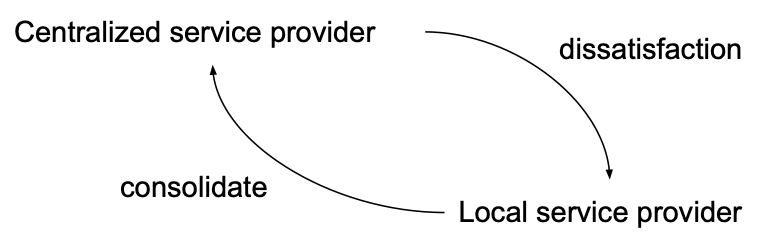
\includegraphics[width=0.8\textwidth]{images/dilemma_centralization-vs-distributed.pdf}
    \caption{Dipole oscillation. See Dilemma~\ref{table:dilemma-org-central-vs-distributed}. Migrating to the opposite paradigm gives people in charge a chance to show their responsiveness to the needs of participants. The rate of oscillation is a measure of institutional memory half-life.}
    \label{fig:central-vs-distributed}
\end{figure}

%  explanation of context for dilemma
Bureaucratic organizations are comprised of teams that provide services to other members of the organization and to subjects. A centralized approach improves efficiency through less redundancy, but also can decrease responsiveness.  
Grove~\cite{1995_Grove} calls the centralized model functional teams.

% How does this relate directly to bureaucracy as defined as shared resource management policymaking?
%The \hyperref[table:dilemma-org-central-vs-distributed]{Dilemma of Centralization of Services}
% How does this effect your relationships with other bureaucrats?
%The \hyperref[table:dilemma-org-central-vs-distributed]{Dilemma of Centralization of Services}
% Are the incentive structures aligned to support one direction or the other?

Centralization is often carried out for the purposes of cost efficiency. The cost savings are due to de-duplication and having less slack. Both of those ``savings'' are a decrease of redundancy, which has a cost when there are unexpected fluctuations in need. 

Another motive for centralization is to concentrate talent within the organization. This can have the unintentional result of silo'ing talent and isolating experts from the people they want to help.

Decentralized manifests as cross-functional teams. Do the compliance officers or financial people or IT support staff work directly on your team locally or are they in a separate team?

Rate of change between centralized and decentralized may be a function of turnover or promotion rates. \marginpar{[Tag] Speculation}

A matrixed organization~\cite{1985_NASA} mixes the centralized approach and cross-functional team.

% as per chapter 8 of Andy Grove's ``high productivity management''
% When deciding between organizing functionally and organizing along business units the right answer is always the other one.


Centralization is an intentional monopolization, with the corresponding decrease in choices. 
Centralization (de-localization) can decrease the value assigned to feedback from people using the service because personal relations are de-valued. 

The weaker feedback, lack of redundancy, and decreased emphasis on relationships motivates the creation of local services. 


\begin{center}
\begin{table}[H] % ht
\begin{tabular}{ | m{\dilemmatablewidth}| m{\dilemmatablewidth} | } 
  \hline
  \textbf{Redundant services in a market.} &
  \textbf{Monopoly service provider.} \\
  \hline
  \textit{Description}: Using a market model within the organization. &
  \textit{Description}:  \\  
  \hline
  \textit{Pros}: Enable customers to choose the best service. &
  \textit{Pros}: Efficiency of a single service. \\
  \hline
  \textit{Cons}: Redundancy. & 
  \textit{Cons}: Might not meet the needs of all customers. \\
  \hline
\end{tabular}
\caption{
\textit{Dilemma of Monopoly.}
\index{dilemma!of monopoly}
Services within an organization. See also figure~\ref{fig:market-vs-monopoly}.
%{\tiny Tag: Design of organization.}
}
\label{table:dilemma-org-market-vs-monopoly}
%GV     "dilemma-org-market-vs-monopoly" [label="redundant services vs monopoly", shape="box"];
%GV     "dilemma-org-market-vs-monopoly" -> "monopoly";
\end{table}
\end{center}


\begin{figure}[H] % ht
    \centering
    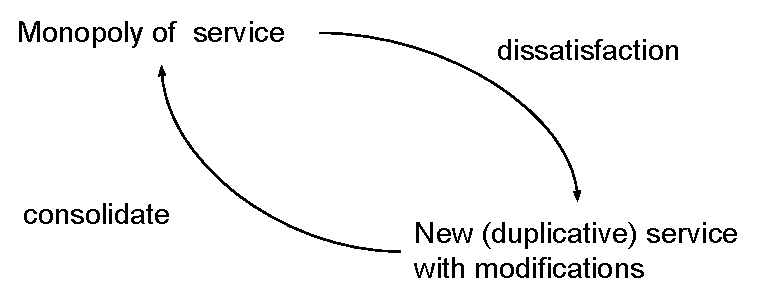
\includegraphics[width=0.8\textwidth]{images/dilemma_market_vs_monopoly.pdf}
    \caption{Dipole oscillation: solution A exists but doesn't meet my needs. Rather than tweak A, re-invent solution B which mostly overlaps with A but has independent development and support. See also Dilemma~\ref{table:dilemma-org-market-vs-monopoly}.}
    \label{fig:market-vs-monopoly}
\end{figure}

% explanation of context for dilemma
The \hyperref[table:dilemma-org-market-vs-monopoly]{Dilemma of Monopoly} is similar to the \hyperref[table:dilemma-org-central-vs-distributed]{Dilemma of Centralization of Services}, in that both seem initially to be dipole oscillations. The centralization of services can be addressed by a matrixed organization, while an approximation of that concept for services would be federation. 

% How does this relate directly to bureaucracy as defined as shared resource management policymaking?
The \hyperref[table:dilemma-org-market-vs-monopoly]{Dilemma of Monopoly} is a label for the tension between minimizing redundancy and customizing solutions. Services tailored to the needs of a bureaucrat or subject mean that someone else with different needs will want a different solution. 

% How does this effect your relationships with other bureaucrats?
%The \hyperref[table:dilemma-org-market-vs-monopoly]{Dilemma of Monopoly}

% Are the incentive structures aligned to support one direction or the other?
The default direction for a bureaucratic organization is towards centralization and monopoly because that seems more efficient. At the same time, individual bureaucrats observe local challenges and invent solutions relevant to their needs.


\ \\

\begin{center}
\begin{table}[H] % ht
\begin{tabular}{ | m{\dilemmatablewidth}| m{\dilemmatablewidth} | } 
  \hline
  \textbf{Decision making lower in a hierarchy.} &
  \textbf{Decision making higher in a hierarchy.} \\
  \hline
  \textit{Description}: Push decisions down to empower employees. &
  \textit{Description}: Escalate every decision to management. \\  
  \hline
  \textit{Pros}: Better information. &
  \textit{Pros}: Better scope. \\
  \hline
  \textit{Cons}: More inconsistency. & 
  \textit{Cons}: Decision maker has less skin in the game and may be less well informed. Employees are disempowered. \\
  \hline
\end{tabular}
\caption{
\textit{Dilemma of Decision Height.}
\index{dilemma!of decision height}
Where decisions get made in hierarchical organization.
%{\tiny Tag: Design of organization.}
}
\label{table:dilemma-org-decisions-low-vs-high}
%GV     "dilemma-org-decisions-low-vs-high" [label="decision making high or low", shape="box"];
%GV     "dilemma-org-decisions-low-vs-high" -> "decisions";
\end{table}
\end{center}

% explanation of context for dilemma
Bureaucrats with direct exposure to a challenge and the ramifications are better positioned to make decisions. As Marquet~\cite{2013_Marquet} points out, pushing decisions down improves the sense of ownership. However, people directly working on a challenge may lack a holistic perspective held by bureaucrats higher in the chain of command. 

% How does this relate directly to bureaucracy as defined as shared resource management policymaking?
The \hyperref[table:dilemma-org-decisions-low-vs-high]{Dilemma of Decision Height} indicates that no individual is ideally positioned to make decisions. Bureaucracy involves distributed decision making because no member has all the relevant information. The coordination of distributed knowledge is a remedy that requires ongoing investment.

% How does this effect your relationships with other bureaucrats?
The \hyperref[table:dilemma-org-decisions-low-vs-high]{Dilemma of Decision height} indicates that relationships up and down the chain of command are necessary. Low-level bureaucrats need to understand the holistic perspective, and bureaucrats at the top of the organization need to understand the ramifications of their decisions.

% Are the incentive structures aligned to support one direction or the other?
Relationships rarely span the chain of command, and bureaucrats make decisions based on locally accessible information and personal experience. 



\ \\

\textit{Trilemma}: \textbf{Do you support the cutting edge, most of the middle, or the laggards?}\\
\index{trilemma!cutting edge, middle, laggards}
For any given aspect of bureaucracy there is a \href{https://en.wikipedia.org/wiki/Normal_distribution}{bell curve} 
\index{Wikipedia!\href{https://en.wikipedia.org/wiki/Normal_distribution}{Normal distribution}}
of skills and interest of bureaucrats. In your role of bureaucrat you face a choice: find and collaborate with and enable the best and brightest, or aim your efforts at the massive mediocre middle (most bureaucrats), or try to get the dumbest bureaucrats up to speed? 

Trying to escape the trilemma by claiming that you treat everyone equally means you are disregarding the needs of the tail of the distribution. 

\ \\

% https://graphthinking.blogspot.com/2021/12/hierarchical-organization-trilemma.html
\textit{Trilemma}: \textbf{Do you work for your team, your manager, or yourself?} \\
\index{trilemma!team, manager, yourself}
Being a member of a team that operates within a hierarchy is tough. One reason is the question of who you are working for. The trilemma is whether you work for yourself, work for your supervisor, or work for your team.  Ideally you can find ways to do all three, but that is not always the case. 

Members of the team should work collaboratively, but there is a potential counter-force: accountability to the supervisor. Because each team member is accountable to their supervisor(s), that motivates the action of the individual. The team does not actually have autonomy -- they are accountable to the boss.

In the approach ``team members are directed by their supervisor," the synergy of the team is neglected and the supervisor becomes a bottleneck (for decision making and for creativity and for planning).

The third approach is for a person to ignore their team and their supervisor. This might enable quicker progress, at the risk of going in an unhelpful direction or not leveraging skills of coworkers. 

\ \\

\textit{Trilemma}:
\textbf{Seek less budget, same, or larger budget.} 
\index{trilemma!less, same, or larger budget}
Less budget is needed if you improved efficiency, but then the proportional power within the organization is decreased. A larger budget may be due to inefficiency or growth. Keeping the same budget indicates no promotions are relevant (although a steady state could result from a combination of growth and improved efficency). 

\ \\

A trilemma applicable to many situations is that options are \textbf{fast, inexpensive, good; choose two}. 
\index{trilemma!fast, inexpensive, good}
(This is the \href{https://en.wikipedia.org/wiki/Project_management_triangle}{Project management triangle}.) 
\index{Wikipedia!\href{https://en.wikipedia.org/wiki/Project_management_triangle}{Project management triangle}}
\\
\index{folk wisdom!\href{https://en.wikipedia.org/wiki/Project_management_triangle}{Project management triangle}}
In other words, the options are
\begin{itemize}
    \item Good and fast is expensive (i.e., requires lots of resources).
    \item Good and inexpensive takes a long time (i.e., find a clever solution).
    \item Fast and inexpensive will be low quality.
\end{itemize}

\subsection*{Dilemmas Raised by Subjects of Bureaucracy\label{sec:subjects-dilemmas}}

%GV } // end org
%GV subgraph cluster_subject {
%GV    label = "subject dilemmas";

Each subject of bureaucracy views themselves as logical and self-consistent and erudite. In practice, the bureaucrat servicing subjects encounters conflicting statements. 

\begin{center}
\begin{table}[H] % ht
\begin{tabular}{ | m{\dilemmatablewidth}| m{\dilemmatablewidth} | } 
  \hline
  \textbf{Subject asks, ``Why do I have to fill out this form?''} &
  \textbf{Subject asks, ``Why aren't you catching more cheaters and fraudsters?''} \\
%  \hline
%  \textit{Description}:  & 
%  \textit{Description}:  \\
%  \hline
%  \textit{Pros}: . & 
%  \textit{Pros}: . \\
  \hline
  \textit{Cons}: Filling out forms is burdensome for the subject and the bureaucrat. & 
  \textit{Cons}: To detect problems and identify risks, information is needed. \\
  \hline
\end{tabular}
\caption{\textit{Dilemma of Forms}: no one likes paperwork or letting cheaters cheat. The cost of protecting scarce resources is felt by everyone.
}
\label{table:dilemma-subject-forms}
%GV     "dilemma-subject-forms" [label="burden of forms", shape="box"];
%GV     "dilemma-subject-forms" -> "forms";
\end{table}
\end{center}

% explanation of context for dilemma
Subjects of bureaucracy expect efficiency. While that's reasonable, the nuances include minimizing the burden of interaction while also making sure the shared resource managed by bureaucrats isn't misallocated to malicious or unworthy recipients. 

The 
\hyperref[table:dilemma-subject-forms]{Dilemma of Forms}
is the subject's experience of the bureaucrat's 
\hyperref[table:dilemma-personal-single-bit-decision]{Dilemma of Redundant Data for Decisions}

% How does this relate directly to bureaucracy as defined as shared resource management policymaking?
%
% How does this effect your relationships with other bureaucrats?
As a result of the \hyperref[table:dilemma-subject-forms]{Dilemma of Forms}, bureaucrats are unable to satisfy the desire of subjects to have efficient bureaucracy. 

% Are the incentive structures aligned to support one direction or the other?


\begin{center}
\begin{table}[H] % ht
\begin{tabular}{ | m{\dilemmatablewidth}| m{\dilemmatablewidth} | } 
  \hline
  \textbf{Subjects desire consistency across situations.} &
  \textbf{Subjects seek exceptions for their specific situation.} \\
  \hline
  \textit{Description}: Predictability allows for planning. & 
  \textit{Description}: I am unique. \\
%  \hline
%  \textit{Cons}: . & 
%  \textit{Cons}: . \\
  \hline
\end{tabular}
\caption{\textit{Dilemma of Consistency.}
Consistency is seen as fairness, when in fact consistency can ignore critical differences. %Consistency is desirable for enabling predictability.
}
\label{table:dilemma-subject-consistency-per-situation}
%GV     "dilemma-subject-consistency-per-situation" [label="consistency vs exceptions", shape="box"];
%GV     "dilemma-subject-consistency-per-situation" -> "consistency";
%GV     "dilemma-subject-consistency-per-situation" -> "exception";
\end{table}
\end{center}

% explanation of context for dilemma
The origin of the \hyperref[table:dilemma-subject-consistency-per-situation]{Dilemma of Consistency} is based in narcissism on the part of subjects. ``I am uniquely special and no one else is.''  

% How does this relate directly to bureaucracy as defined as shared resource management policymaking?
%T
% How does this effect your relationships with other bureaucrats?
%The \hyperref[table:dilemma-subject-consistency-per-situation]{Dilemma of Consistency}
% Are the incentive structures aligned to support one direction or the other?
Bureaucrats seek consistency in the application of policies as a defensible story justifying the allocation of shared resources. A complicating factor is whether you think of fairness as equality (consistency means everything is the same) or equity (consistency accounts for differences). 

As with the \hyperref[table:dilemma-subject-forms]{Dilemma of Forms}, the consequence of the \hyperref[table:dilemma-subject-consistency-per-situation]{Dilemma of Consistency} is that subjects will usually be unhappy with bureaucracy. 

\begin{center}
\begin{table}[H] % ht
\begin{tabular}{ | m{\dilemmatablewidth}| m{\dilemmatablewidth} | } 
  \hline
  \textbf{Subjects seek clearly defined rules.} &
  \textbf{Subjects seek flexibility in application of rules.} \\
  \hline
  \textit{Description}: Rules are seen as enabling fairness, when in fact rules can perpetuate inequality. Rules (assuming uniform enforcement) are also seen as enabling predictability. & 
  \textit{Description}: Subject may expect their status in the community or their relationship with the bureaucrat enables exceptions. \\
%  \hline
%  \textit{Pros}: . & 
%  \textit{Pros}: . \\
%  \hline
%  \textit{Cons}: . & 
%  \textit{Cons}: . \\
  \hline
\end{tabular}
\caption{\textit{Dilemma of Flexible Rules.}
}
\label{table:dilemma-subject-flexibility}
%GV     "dilemma-subject-flexibility" [label="clear rules vs flexiblity", shape="box"];
%GV     "dilemma-subject-flexibility" -> "flexibility";
\end{table}
\end{center}

%  explanation of context for dilemma
The application of policy by bureaucrats is subjective. Relying on rules to be deterministic misses the relevance of human interpretation. Predictability of rulings can benefit bureaucrats and subjects.

% How does this relate directly to bureaucracy as defined as shared resource management policymaking?
% How does this effect your relationships with other bureaucrats?
As with all other dilemmas, the \hyperref[table:dilemma-subject-flexibility]{Dilemma of flexible rules} is enacted to various degrees by different bureaucrats, resulting in non-uniform outcomes for subjects. Your relationship with the deciding bureaucrat matters. Information you provide and arguments you make sway the decider. 

% Are the incentive structures aligned to support one direction or the other?
The bias for bureaucrats faced with the \hyperref[table:dilemma-subject-flexibility]{Dilemma of flexible rules} is to appear consistent across decisions. The appearance of inconsistent policy application is harmful to the reputation of the bureaucrat and the organization.

\begin{center}
\begin{table}[H] % ht
\begin{tabular}{ | m{\dilemmatablewidth}| m{\dilemmatablewidth} | } 
  \hline
  \textbf{Subject wants transparency.} &
  \textbf{Subject wants low cost (free).} \\
  \hline
  \textit{Description}: Transparency requires collection and reporting of data. & 
  \textit{Description}: Access to shared resources shouldn't be costly. \\
%  \hline
%  \textit{Pros}: . & 
%  \textit{Pros}: . \\
%  \hline
%  \textit{Cons}: . & 
%  \textit{Cons}: . \\
  \hline
\end{tabular}
\caption{\textit{Dilemma of transparency.}
Transparency has a cost.
}
\label{table:dilemma-subject-transparency}
%GV     "dilemma-subject-transparency" [label="transparency vs low cost", shape="box"];
%GV     "dilemma-subject-transparency" -> "transparency";
\end{table}
\end{center}

% explanation of context for dilemma
Whenever there is a desire for lower cost and some feature there is a tension with the costly feature. Bureaucrats make subjective decisions, so transparency helps other people understand the reasoning behind outcomes. Transparency is not free, so a dilemma occurs. 

% How does this relate directly to bureaucracy as defined as shared resource management policymaking?
%The \hyperref[table:dilemma-subject-transparency]{Dilemma of transparency}

% How does this effect your relationships with other bureaucrats?
The \hyperref[table:dilemma-subject-transparency]{Dilemma of transparency} depends on your role. If you are a decision maker or data owner, you do not gain immediate value from justifying decisions or sharing data. You pay a cost to provide transparency, both reputational (your mistakes become visible) and financial (for hosting data, time spent publishing). There are potential benefits to transparency -- improved trust in relationships, subjects detecting and reporting mistakes. 

% Are the incentive structures aligned to support one direction or the other?
An incumbent bureaucrat defaults to no transparency. If subjects want to dispute decisions they benefit from having information about how the policy was applied. If the subject is willing to pay the cost for the data, then the decision maker has to do extra work to make data available.


\subsubsection*{Consequences of the Dilemma-based Framing}

There are many dilemmas listed above but the list is not comprehensive. Even if each bureaucrat considers the same choices (which doesn't necessarily happen), not everyone makes the same selection. 

To avoid dilemmas, a response might be to defer to someone higher in the hierarchy to decide and coordinate. While fewer people making decisions would improve consistency, this would be \href{https://en.wikipedia.org/wiki/Micromanagement}{micromanagement}. 
\index{Wikipedia!\href{https://en.wikipedia.org/wiki/Micromanagement}{micromanagement}}
The people in the hierarchy above the person facing the choice don't have exposure to the problem. Choices are delegated to leverage expertise. 

\ \\

When you are facing these dilemmas and trilemmas
\marginpar{[Tag] Actionable Advice} 
\index{actionable advice}
there are constructive responses that can improve your effectiveness. Improvement benefits your results, your reputation, and the organization. 
\begin{itemize}
    \item Collect quantitative data for each variable. Quantitative arguments can augment qualitative stories. 
    \item Construct the Pareto frontier to identify non-optimal choices that can be eliminated.
    \item Instead of assessing variables in isolation, assess consequences in the context of workflows and effects on stakeholders.
    \item Discuss subjective decisions with stakeholders so that potential disagreements can be negotiated instead of creating friction.
\end{itemize}
 

%GV } // end subject subgraph
%GV } // end digraph G \clearpage
  \section{Unavoidable Hazards of Bureaucracy\label{sec:unavoidable-hazards}}

There are certain challenges in a bureaucracy that cannot be avoided. The value of recognizing them is to understand that what you're experiencing isn't an anomaly. The problem isn't unique to you, your circumstances, your coworkers, or the organization. The cause is the combination of all those factors.

Good ideas are not enough for adoption or continuation.
Concepts critical to the success of the organization do not need to continue. Emotional fortitude is critical.


\ \\
\begin{samepage}
\textit{Hazard}: \textbf{Separation of responsibility and accountability}. \\
Each bureaucrat in an organization has responsibilities associated with their role. The ability to complete the tasks associated with the role is not wholly within the scope of the bureaucrat's control. You are dependent on other bureaucrats. Even if there is a desire for action, the action might not be immediately feasible because of a dependence on another person or process. 

The consequence of separation of responsibility from authority is that other people look incompetent or lazy and unresponsive.
\end{samepage}

\ \\
\begin{samepage}
\index{mantra!perception matters more than intent}
\textit{Hazard}: \textbf{Perception matters more than intent}. \\
You may mean to convey a specific message, but the way your listeners hear that content or read the message depends on context and interpretation. 
Decreasing the ambiguity in phrasing is a useful investment, but you don't control how an audience responds. 

Communication is crucial for bureaucracy, so the best response is iterating with an audience rather than expecting a single message to be sufficient. 
\end{samepage}

\ \\
\begin{samepage}
\textit{Hazard}: \textbf{Appreciation for being an effective bureaucrat is rare.}\\
If you do your job well no one will notice. This is because of an expectation of smooth and fast interactions. Frictionless engagement is expected even if that is not the norm. 

Consider teachers who catch cheating students:
\begin{quote}
``No one [thanks teachers] for policing cheating. Not the cheaters, not the honest students who feel inconvenienced and mistrusted, and certainly not the school [administrators] who have to process academic dishonesty paperwork.''\footnote{\href{https://dynomight.net/teaching/}{https://dynomight.net/teaching/}.}
\end{quote}
\end{samepage}

This same concept applies to any bureaucrat. The number of thank you cards sent to \href{https://www.fda.gov/}{Food and Drug Administration} meat inspectors keeping food safe, \href{https://www.osha.gov/}{Occupational Safety and Health Administration} regulators ensuring a safe work environment, \href{https://www.fcc.gov/}{Federal Communications Commission} detecting disruptive electromagnetic signals, \href{https://www.ftc.gov/}{Federal Trade Commission}, and \href{https://www.sec.gov/}{Securities and Exchange Commission} is likely small.\footnote{FoIA 2022-000758 submitted to the \href{https://www.fcc.gov/}{Federal Communications Commission}  
sought the first 100 documents received by the FCC from consumers with any of the words ``thank,'' ``thanks,'' ``appreciate,'' or ``appreciated'' between January 1, 2020 to December 31, 2020. 
I reviewed the 100 documents and found no letter of gratitude; just complaints.}
% POTENTIAL task: ask each agency how many thank you letters they receive
% FOIA SSA-2022-01  5009
% FOIA FCC-2022-000758

There are counterexamples in public service bureaucracy. 
Law enforcement is thanked when there is a victim of a crime. 
\index{exemplar!law enforcement officers (LEO)}
The military is held in high regard. 
\index{exemplar!military}
In both of those bureaucracies the bureaucrats are visible and the consequence of their work is tangible. 

In large organizations there are teams of bureaucrats like the Information technology department and human resources. IT support bureaucrats are occasionally thanked by their subjects, though most of the time the expectation is that computers should just work. HR produces no tangible products, so the appreciation is lower.


\ \\
\begin{samepage}
\textit{Hazard}: \textbf{Lack of accountability to fellow bureaucrats who rely on you.}\\
You are more likely to feel accountable to your supervisor. Performing for your supervisor and explaining your value matters more than the work done to support coworkers.  This also applies when you depend on other people -- they aren't accountable to you.

To counter this tendency, build personal relationships with peers. This requires ongoing investment, both to maintain relationships and to create bonds with new coworkers as your previous coworkers leave.
\end{samepage}

\ \\
\textit{Hazard}: \textbf{Decision-makers are under-informed and inexperienced.}\\
You can make a decision with insufficient information. There is rarely an expectation of expertise or experience. 
Gathering information takes time and is thus burdensome.
Having experience requires getting experience -- you either start as a novice and make mistakes, have formal academic training, or rely on mentorship to avoid the direct experience of mistakes.

\ \\
\textit{Hazard}: \textbf{Gathering data for decisions takes resources and expertise.}\\
When there is a desire to gather data, and there is data available to be gathered, an investment of time is necessary. Well-informed decisions take time, experience, or both.

\ \\
\textit{Hazard}: \textbf{Defining success is subjective and dynamic}. \\
Who defines success and for which audience in a bureaucratic organization is subjective because of the lack of feedback mechanisms. Consequences may not be immediately obvious. Worse, how success is defined can be changed at any time -- there's no need for consistency. 

\ \\
\textit{Hazard}: \textbf{Change threatens incumbents}. \\
Change of plans, roles, tasks, resources, the flatness of the organization, scope, technology.

\ \\
\textit{Hazard}: \textbf{\href{https://en.wikipedia.org/wiki/Diffusion_of_responsibility}{Diffusion of responsibility} 
\index{Wikipedia!\href{https://en.wikipedia.org/wiki/Diffusion_of_responsibility}{Diffusion of responsibility}}
in the bureaucracy}. \\
A specific task needs to be completed, and action requires the involvement of multiple collaborators. 


Consider the perspectives of an office worker, an office manager, a building manager, an electrical substation operator, and an electrical grid operator.
\begin{center}
\begin{figure}
    \centering
    % left> <lower> <right> <upper
    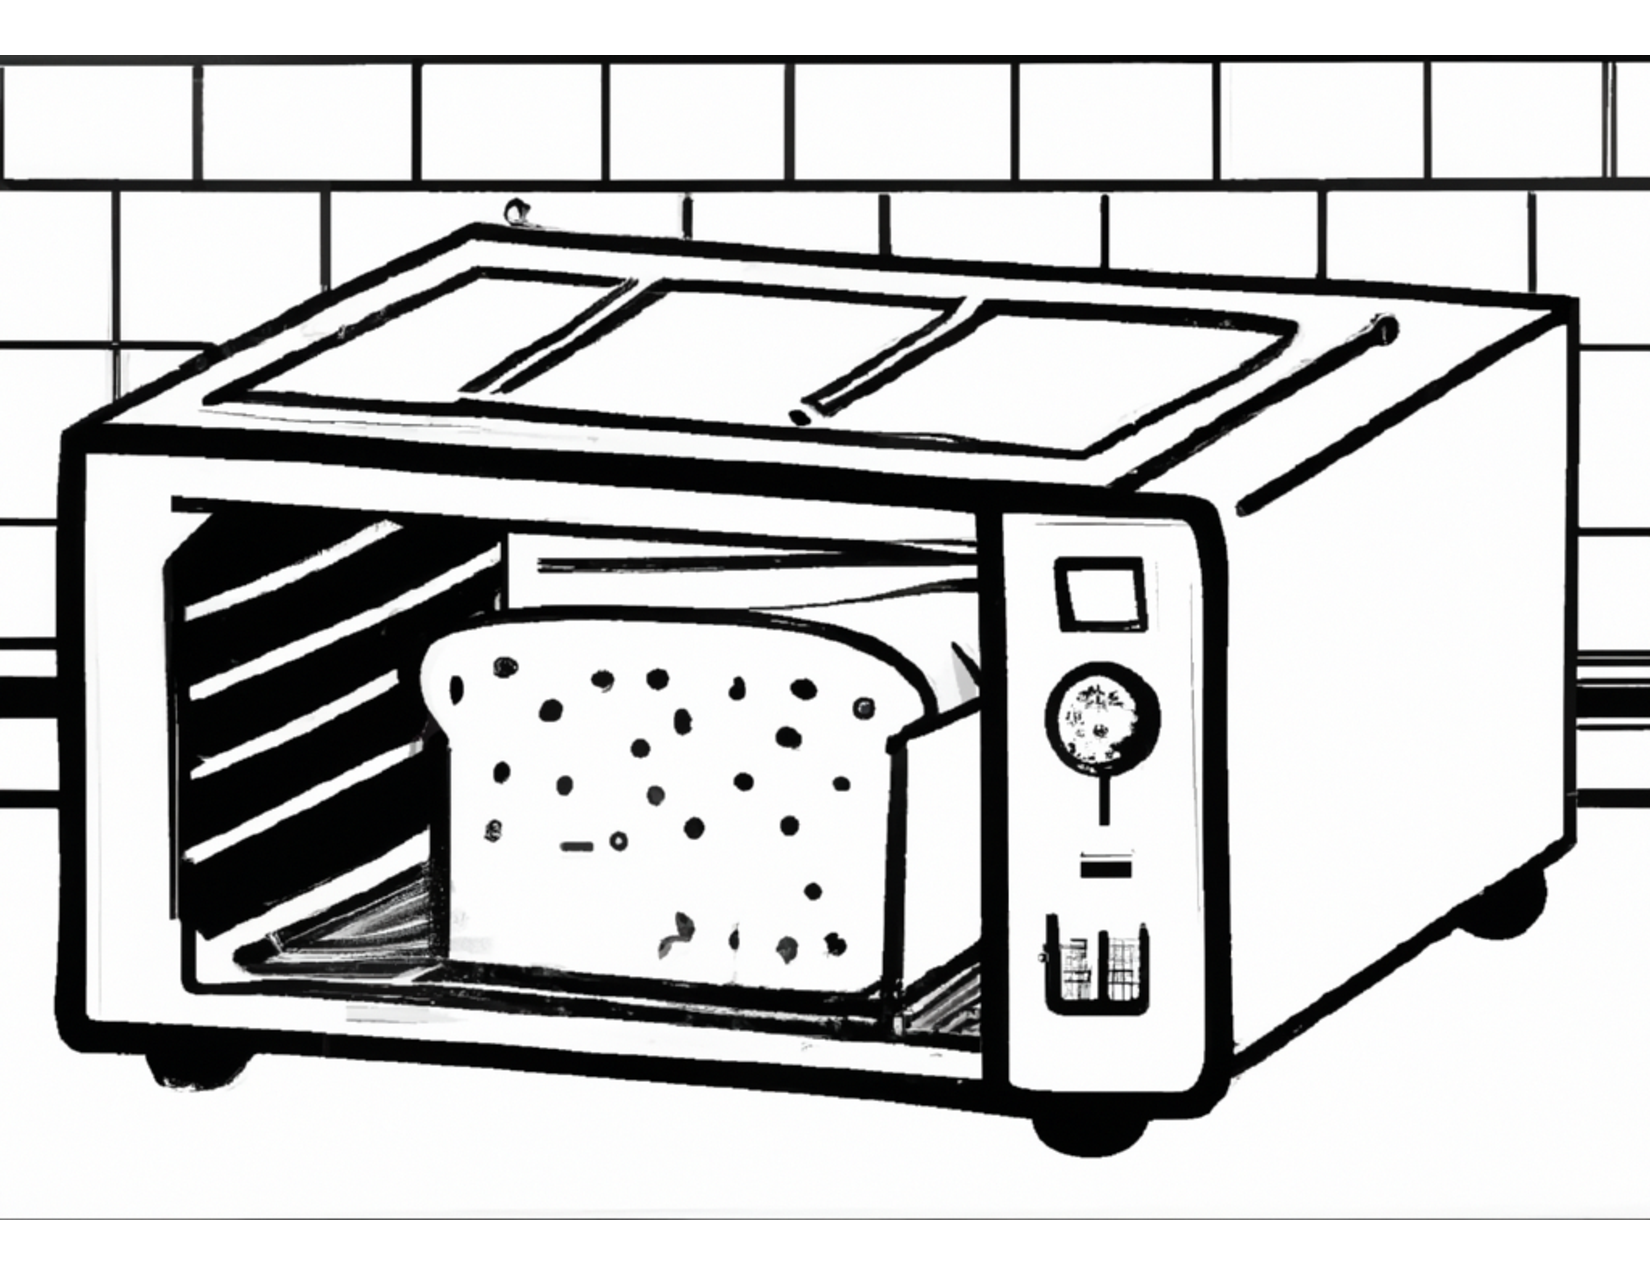
\includegraphics[width=0.7\textwidth,trim={0 2cm 0 0},clip]{images/toaster_oven_in_office_kitchen.pdf}
    \caption{Toaster oven in the office kitchen.}
    \label{fig:toaster_oven}
\end{figure}
\end{center}

\index{story time!layers of margins}
%\marginpar{[Tag] Story Time}
%\begin{storytime}{Layers of Margins}
\begin{mdframed}[frametitle={Layers of Margins},frametitlerule=true,frametitlealignment=\centering]
An office worker wants to plug in a toaster oven in the office kitchen (see figure~\ref{fig:toaster_oven}). The owner of the toaster oven files a notice with the office manager who tracks electrical loads in the kitchen. 
The toaster owner uses the power number (1200 \href{https://en.wikipedia.org/wiki/Watt}{Watts}) 
\index{Wikipedia!\href{https://en.wikipedia.org/wiki/Watt}{Watts}}
from the manufacturer's website. In practice the toast oven doesn't actually use that much power; that's just the maximum rating for the device. 

The office manager aggregates power from the devices in the kitchen. The office manager has a power budget for the team's kitchen equipment and keeps a margin of 10\% spare capacity for flexibility. The office manager's power budget is provided to the building manager (who keeps a margin of 10\% for flexibility). The building is one of many sharing the electrical substation. The electrical substation owner sees the power consumption is below the rated capacity, but the subscription for available power is full -- no new users can be supported.
%\end{storytime}
\end{mdframed}
Lesson: in a system of aggregated layers, each person only sees adjacent layers. When each person builds safety into their budget, the accumulated slack is excessive and wasteful.

Similar situations arise for temporal planning (schedule), financial budgets, and spatial planning. 

%Once responsibility is assigned, the new risk is that of blame.

\ \\
\textit{Hazard}: \textbf{Diffusion of blame in the bureaucracy}. \\
Example: if something goes wrong, who is at fault: the creator of a policy or the person tasked with executing the policy?

\ \\
\textit{Hazard}: \textbf{High latency feedback}. \\
See 
\hyperref[sec:slowing-communication]{slow communication}\iftoggle{haspagenumbers}{ on page~\pageref{sec:slowing-communication}}{} 
and 
\hyperref[sec:decision-delay]{decision delay}\iftoggle{haspagenumbers}{ on page~\pageref{sec:decision-delay}.}{.}

\ \\
\textit{Hazard}: \textbf{Weak feedback}. \\
Suppose my bureaucratic task depends on a service provided by you, a fellow bureaucrat. If your computer isn't working, your ability to provide the service is blocked by a dependency on a computer repair person. You might feel relieved -- you can relax while you wait on the computer repair and you don't have to do work providing the service to me. You might feel anxious -- you're unable to provide the service until the computer is fixed. Regardless of how you feel about the situation, my task is blocked. If neither you nor I have priority relative to the computer repair person's other tasks, then we wait. This question of priority could be resolved hierarchically (for which there is limited attention bandwidth) or socially (dependent on someone having a relationship with the repair person). 

The delay for my task may be sufficiently small that raising the issue through the hierarchy or socially is not a good use of time.

\ \\
\textit{Hazard}: \textbf{The person making the rules that you follow doesn't actually know what they're doing}. \\
Your choices then include
\begin{itemize}
    \item Follow the rules that are not correct. This harms your productivity and morale. 
\item You can violate the rules and be more effective. This puts you at risk for sanctions. 
\item You can work the change the rules. Then you are not doing the work that's needed.
\end{itemize}


\ \\
\textit{Hazard}: \textbf{You rarely get to pick who is on the team}. \\
When a task requires collaboration, there is rarely a choice of who you get to work with. 

\ \\
\textit{Hazard}: \textbf{You rarely get to alter team membership.}\\
As a team member, you typically get little input on who you work with. Even as a manager your options for hiring are often limited. 

\ \\
\textit{Hazard}: \textbf{Fear of the unknown.}\\
Current suffering is tolerable compared to the uncertainty of change, especially when the suffering isn't felt by the decision-maker.

By identifying this fear in yourself or those you collaborate with, you can discuss specific concerns and work to address them.
\marginpar{$>>$ Actionable Advice} 
\index{actionable advice}

\ \\
\begin{samepage}
\textit{Hazard}: \textbf{Fear of change.} \\
Change disrupts the status quo, putting accumulated power at risk and altering relationships. 
\end{samepage}

An emotional basis for decision-making (or avoidance of decision-making) may or may not be rational. Discussing the fear with fellow bureaucrats can ease the burden. 

\ \\
\textit{Hazard}: \textbf{Fear of conflict.}\\
Refers to conflict of ideas, not physical conflict. Conflict of ideas is not personal, though the consequences may have impacts on careers for stakeholders. \\
Professional disagreement is to be expected in a bureaucratic organization.

Feeling uncomfortable is distinct from feeling unsafe. Communicating while feeling discomfort is a useful skill, rather than avoidance. You can demonstrate courage by talking about your sense of discomfort. 

\ \\
\textit{Hazard}: \textbf{Inadequate resources: staffing, time, money.}\\
The resources you have to address a challenge may not match the complexity of the issue.

\ \\
\textit{Hazard}: \textbf{Outcomes for the team are ill-defined and constantly shifting.}\\
Most bureaucrats rely on approaches that assume consistency of their environment. Planning for uncertainty and change is more complicated.

\ \\
\textit{Hazard}: \textbf{The reward for good work is more work.}\\
When a coworker doesn't do their fair share, then the productive employee shoulders more burden. The deficient worker has no incentive to improve.

\ \\
\textit{Hazard}: \textbf{The organization has a lack of vision; or has vision but no plan; or has vision and a plan but no consensus; or has vision and a plan and consensus but inadequate resources.}\\
An organization of bureaucrats can operate without a vision, plan, or sufficient resources. Being busy is easy; being productive is hard.
\index{mantra!busy is easy, productive is difficult}

\ \\
\textit{Hazard}: \textbf{Progress depends on subjective decision-making.}\\
Rarely is the optimal path deterministic. 

\ \\
\textit{Hazard}: \textbf{Easier to ask for big money than small money.}\\
Processes are scale invariant. Regardless of whether you're asking for \$1000 or \$100,000, the process is the same. Accountability processes for large amounts of money are not scaled down to fit small amounts because people can be as dumb with \$100 as they are with \$10,000.


People problems are invariant of where in the hierarchy the problems occur. Less attention is paid to the same problem at the lowest levels as compared to higher in the hierarchy.
%The challenges observed in bureaucracy are scale invariant
%It doesn't matter how many people you have to manage
%It doesn't matter how many zeros are in your budget


\ \\
\textit{Hazard}: \textbf{Flux of people and processes.} \\
Sources of flux include staff turnover, changing conditions, changing timelines, change of vision, and the need to be promoted. Consistency doesn't yield promotion in a bureaucracy.

\ \\
\textit{Hazard}: \textbf{Why are there so many rules?}\\
To address edge cases and malicious or dumb people. See the \hyperref[table:dilemma-subject-forms]{Dilemma of Forms}.
\marginpar{See page~\pageref{table:dilemma-subject-forms}.}

\ \\
\textit{Hazard}: \textbf{So much paperwork or forms.}
Why is red tape endemic to bureaucracy?\\
Paperwork as a form of coordination in processes to facilitate decentralized decision-making. 

One of the motives for paperwork is to catch people who are misrepresenting their intent, whether accidental or intentional. Documentation makes prosecution more straightforward.

\ \\
\textit{Hazard}: \textbf{Everything is slower.}\\
What the person saying this means is ``slower than desired for what I need" or ``slower than I imagined in my simplified model."

Progress is slower than expected because there aren't as many hours available as na\"ively imagined. The actual time spent working in a bureaucracy is less than the number of hours you get paid for. Breaks taken during work, vacation from work, holidays, and sick leave are illustrated in figure~\ref{fig:hours_per_year}. An additional factor is that the people you depend on do not work exclusively on your request -- there are competing investments of attention. 

Developing \gls{process empathy} means having a more detailed model that accounts for the cost of coordination and accounts for there being less time available than the na\"ive expectation. 

% https://rescuetime.wpengine.com/work-life-balance-study-2019/

\begin{figure}[!htb] %[H]
    \centering
    \includegraphics[width=0.8\textwidth]{images/hours_per_activity_per_employed_year}
    \caption{Hours of ``work'' per year when accounting for the rest of life. Assumes five weeks of vacation, two days of sick leave, and eleven holidays.}
    %\href{https://docs.google.com/spreadsheets/d/1ZaOZZXWkEzX4fFltUdlR4A6ENrAXnkzTW4YrjA4tDO8/edit?usp=sharing}{source for calculations}
    % footnotes in caption is not recommended; see https://texfaq.org/FAQ-ftncapt
    % however it can be done; see https://stackoverflow.com/questions/67621322/footnote-in-caption-of-figure-on-latex
    \label{fig:hours_per_year}
\end{figure}

\ \\
\begin{samepage}
\textit{Hazard}: \textbf{Bureaucracy inhibits creativity.}\\
See 
%section~\ref{sec:innovation} for 
notes on 
\hyperref[sec:innovation]{innovation}\iftoggle{haspagenumbers}{ on page~\pageref{sec:innovation}.}{.}
\end{samepage}

\ \\
% https://graphthinking.blogspot.com/2017/06/measuring-growth-of-bureaucracy.html
\textit{Hazard}: \textbf{Bureaucracy grows.}\\
The causes of growth include
scope creep, an increased number of people participating in the process, an increased workload, or the ratio of workers to managers decreases. 

Bureaucracy grows because some people lie. 
The progress is called ``improved accountability" because we aren't sure who the next liar is going to be.
More work is created for everyone because we don't want to confront  liars and cheaters. 


You can measure the growth of bureaucracy using metrics like the latency in addressing a request and the number of people involved in addressing a request.  

\textbf{Increasing the size of a bureaucracy is easier than cutting it down.}\\


\ \\
% https://graphthinking.blogspot.com/2017/04/growth-of-bureaucracy.html
\textit{Hazard}: \textbf{The ratio of workers to managers gets worse as the size of the hierarchy grows}. \\
As complexity and workload increase, the number of staff needed increases. To facilitate coordination, managers arise. The amount of work being done in a bureaucracy can be small compared to the number of participants.

In figure~\ref{fig:growth_of_bureaucracy}a, the ratio of workers to participants is 3:3=1. When a manager is added, the ratio is 3:4 = 0.75 (a lower value means less apparent work per employee is being done). Adding a second team with dedicated management puts the ratio at 6:9=0.66. Finally, with a dedicated administrative team (e.g., payroll, hiring, facilities), the ratio is 6:13=0.46.

Adding more people to a hierarchical organization results in diminishing returns for time spent on the central work since bureaucrats invest time maintaining the hierarchy and administrative processes.

% TODO: make a better diagram, 
% TODO: plot ratio as function of depth for various branching
    \begin{figure}
        \centering
        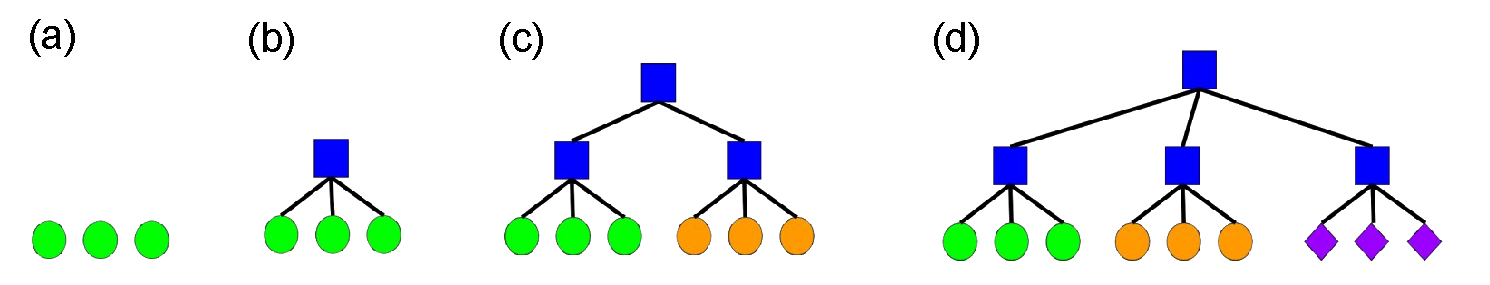
\includegraphics[width=1\textwidth]{images/growth-of-bureaucracy.pdf}
        \caption{Growth of an organization as complexity and workload increase. a: three technical workers (green dots); b: administrative functions are delegated to an administrative assistant or manager (blue square); c: as complexity and scale grows, a new technical team (orange dots) is brought in which has their own manager; d: administrative work is delegated to a dedicated team of non-technical staff (purple diamonds).}
        \label{fig:growth_of_bureaucracy}
    \end{figure}

\ \\
\textit{Hazard}: \textbf{Each person in a bureaucracy has multiple roles}.\\
To limit the expansion of the bureaucracy. The multiple roles come from multiple relationships necessary to span an organization larger than \href{https://en.wikipedia.org/wiki/Dunbar\%27s_number}{Dunbar's number}. \iftoggle{WPinmargin}{\marginpar{[Wikipedia] Dunbar's\\number}}{}
\index{Wikipedia!\href{https://en.wikipedia.org/wiki/Dunbar\%27s_number}{Dunbar's number}}

\ \\
\begin{samepage}
\textit{Hazard}: \textbf{Everything is more complicated}. \\
Bureaucracy administers access to resources, whether tangible items (water, air) or expertise. There's friction for tangible resources because the easiest solution is you get the resource (without an intermediary). There's friction for expertise because the expert understands things you do not. 
\end{samepage}

\ \\
\textit{Hazard}: \textbf{Bureaucracy is inefficient and wasteful.}\\
The inefficiency of an organization is not just due to a breakdown of communication among its many members. Other sources include 
\begin{itemize}
    \item Individuals in different roles face distinct external incentives which drive a diversity of investments. Work that is not aligned results in wasted effort.
    \item Participants have a different views of what constitutes a problem and which problem is most relevant. Coordinating to resolve disagreements appears inefficient regardless of which metric is used to measure efficiency.
    \item Within the organization there can competition  for resources. Competition leads to wasted effort.
    \item Because decisions by bureaucrats are subjective, there is significant risk of being wrong or being called out by others as being wrong. The incentive to 
\href{https://en.wikipedia.org/wiki/Cover_your_ass}{
cover your ass}\footnote{
\cite{1996_unknown}: ``the preferred options are to make sure somebody else does the failing, or to elegantly explain why it looks like a failure, sounds like a failure, but is actually a brilliant advance in an unexpected direction.''}
\index{Wikipedia!\href{https://en.wikipedia.org/wiki/Cover_your_ass}{
cover your ass}}\iftoggle{WPinmargin}{\marginpar{[Wikipedia] Cover\\your ass}}{}
exists for decisions. As a result, unnecessary work is carried out to limit blame. 
\item Situations and constraints change faster than the time it takes to complete a task.  Then you are faced with either continuing under the initial assumptions or pivoting a project partway through. If an objective quantitative measure of value is available, the return on investment could be determined.
\end{itemize}


Efficiency is typically assessed from the perspective of a serial process -- a single worker could do this task faster, so why involve ten people and get a slower, more burdensome result? Specialization of skills, resilience, validation checks, and increased throughput all  motivate the addition of bureaucrats to processes.

Brook's Mythical Man Month~\cite{1975_brooks} points out that dividing a task among ten people does not make the task finish in a tenth of the time. There is overhead of coordination and the training of new members who are intended to help. 

\href{https://en.wikipedia.org/wiki/Amdahl\%27s_law}{Amdahl's law}
\index{Wikipedia!\href{https://en.wikipedia.org/wiki/Amdahl\%27s_law}{Amdahl's law}}
is the quantification that a task which takes one person one hour is unlikely to scale to ten people accomplishing ten results in one hour.
The consequence is that you can't evaluate what should be considered wasteful by considering a single person's throughput and then multiplying by the number of people on a team.


%Inefficiency of process is similar. I need to file a request to replace the lightbulb in my office. Compared to the serial ``I'll just replace the lightbulb myself by running to the hardware store and purchasing one."



\ \\
% https://graphthinking.blogspot.com/2020/07/scope-creep-is-experienced-differently.html
\begin{samepage}
\textit{Hazard}: \textbf{Scope creep.}\label{sec:scope-creep} \\
Scope creep can originate from three sources: the bureaucrat doing the work, the customer of the bureaucrat's work, and the bureaucrat management. In the first situation, the person doing the work might see a nearby opportunity that only requires a little be more work. 
\end{samepage}

When the customer is the source of scope creep, the root cause is that customer wants more. While the exploration of what's possible can be exciting (a positive experience), what the bureaucrat hears is more work and delayed results. This implies a few trade-off options, all of which are negative for one or both parties.
\begin{itemize}
    \item Stick with the original terms (telling the customer ``no", which is negative for both parties).
    \item Re-negotiation for more time (a burden to both parties).
    \item The bureaucrat doing more for the same pay, which means less money per effort (yielding a less happy bureaucrat).
    \item Decreasing existing efforts to fit the added requirements (yielding a less happy customer).
    \item Even if the bureaucrat is getting paid by the hour, more work means the end product will be delayed to accommodate added features (yielding a less happy customer).
\end{itemize}

The third source of scope creep is from management. Executive decision-makers tried to make decisions without having the full context of the impacts of the decisions. Lower level people doing things see opportunities and extend their scope incorrectly because they don't have the full picture. In both these cases, the problem is that the person doesn't know what they don't know and trying to solve problems outside of their knowledge. How would that person know that they don't know? The easy answer to this is if you are in a position of authority, check downward before making a pronouncement. If you are in a position of execution, check upward before taking action. \href{https://en.wikipedia.org/wiki/Intent_(military)#Commander's_intent}{Commander's intent}
\index{Wikipedia!\href{https://en.wikipedia.org/wiki/Intent_(military)#Commander's_intent}{Commander's intent}}
works in both directions.

\ \\
% https://graphthinking.blogspot.com/2020/09/why-migrating-from-current-to-new.html
\textit{Hazard}: \textbf{Migrating technologies.} \\
The person enacting the transition has to be educated in both the old and new technology. 
The legacy code has to be migrated to the new implementation
convincing stakeholders; may require synchronization
difficulty scales with the number of stakeholders  \clearpage    

\chapter{You are an Individual in an Organization\label{sec:individual-in-org}}
  {\footnotesize Back to the \hyperref[sec:toc]{Main Table of Contents}}
  \minitoc
    This section focuses on an individual bureaucrat operating within an organization. What actions can you take?  This chapter is a prelude to the next chapter, 
    \hyperref[sec:working-with-other-bureaucrats]{working with others}.
    \marginpar{See page~\pageref{sec:working-with-other-bureaucrats}.}
    
    As a bureaucrat, understanding your options for action matters. If you don't know what your options are, you're less effective. If you are ok with being ineffective, or are not feeling the harm of your ineffectiveness, keep in mind that
    there is no neutral member of a bureaucracy. Either you are contributing to the organization, or you are sapping resources from the organization. This is because the organization operates in a zero-sum game for resource allocation.

    
%See also 
% "Making of a Manager" has Chapter 7 (pages 161-187) on hiring

% https://graphthinking.blogspot.com/2019/06/standard-issues-that-organization-must.html
Voluntary membership in a long-lasting organization implies a turnover rate. Organizations constantly have to onboard new members just to maintain a constant level of membership.

An organization is distinct from the rest of society due to the differences in norms and goals. If an organization does not invest in onboarding, the norms of wider society will prevail and the organization will cease to be distinguishable from society.

%In section~\ref{sec:hiring} 
I discuss \hyperref[sec:hiring]{hiring}
\marginpar{See page~\pageref{sec:hiring}}
from both the perspective of the person hiring and the person being hired. 
%In section~\ref{sec:promotion} 
I describe incentives for \hyperref[sec:promotion]{promotion}
\marginpar{See page~\pageref{sec:promotion}}
from both the view of the person promoting a bureaucrat and the person seeking promotion. 
%In section~\ref{sec:professional-training} 
%I explain the relevance of \hyperref[sec:professional-training]{professional training}
%\marginpar{See page~\pageref{sec:professional-training}}
%from the perspective of the employer and the employee. 
My intent is to help people in each position build empathy with the other person's experience. 


\section{Hiring into a Bureaucracy\label{sec:hiring}}


Hiring shapes the culture of an organization and determines what is feasible, both by the skills of those hired and how well new hires integrate with the existing organization. 

Hiring is an expensive process in terms of money, time, emotional investment of candidates, and the burden of reviewing applicants. 
% SO WHAT? What's the consequence?
As a candidate, recognize the risk the organization is taking. 
As a reviewer of candidates, this is an investment in the future of the organization. Even if your bureaucratic role does not require an exclusive focus on hiring, there is value in studying this domain. 

When hiring into an organization there is a selection bias in the people who join a bureaucracy, and there is a selection bias who stays in bureaucracy. 
% SO WHAT? What's the consequence?

% https://leadership.garden/onboarding-engineers/
% https://news.ycombinator.com/item?id=30810786

Regardless of the specifics of the job, there are specific attributes that make a candidate more likely to be successful in a bureaucracy. In addition to role-specific skills, hire for \href{https://en.wikipedia.org/wiki/Metacognition}{metacognition},
\index{Wikipedia!\href{https://en.wikipedia.org/wiki/Metacognition}{metacognition}}
social skills, and intrinsic motivation.

% https://graphthinking.blogspot.com/2021/04/screening-for-metacognition-in-job.html

% https://graphthinking.blogspot.com/2021/07/screening-for-intellectual-empathy-in.html

% https://graphthinking.blogspot.com/2021/04/questions-to-ask-interviewer-when.html

 \clearpage
    \section{Tips for Getting Started}

% https://graphthinking.blogspot.com/2019/11/formal-education-for-domain-exposure.html
You may have graduated from school with a degree in a specific subject. Then you go to work and expect the position you're in to apply the domain-specific education you have in your new role. Your work produces an outcome and gives meaning to the struggle of your prior education process (an investment of time, money, and effort). In practice, there can be a disconnect between your professional role and your educational training. The disconnect may feel dissatisfying when you are not practicing what you went to school for.

An alternative framing that is more helpful is that you went to school to learn how to learn. A degree represents your ability to learn and persist rather than a domain specialization. Then, when you get to work, you are presented with new opportunities to learn other domains. 

\subsection*{Onboarding into a Bureaucratic Organization}

The hiring process involves at least two people. Responsibility for successful integration relies on both people actively working together. This cooperative effort manifests in a few specific tactics. 

\ \\
%\begin{minipage}{\textwidth}
As the new hire, try to learn the names of those around you. %\\
\marginpar{$>>$ Actionable Advice}%
\index{actionable advice}%
As the hirer, make introductions. Not just the first time, but for the first week or two.
%\end{minipage}

\ \\
%\begin{minipage}{\textwidth}
As the new hire, learn the jargon of your new organization. %\\
As the hirer, explicitly expand jargon when used.
%\end{minipage}

\ \\
%\begin{minipage}{\textwidth}
As the new hire, seek one-on-one meetings to get feedback. %\\
As the hirer, offer one-on-one meetings to provide feedback.
%\end{minipage}

\ \\
%\begin{minipage}{\textwidth}
As the new hire, write documentation on processes as you experience them. You're in the best position to write down your observations because you are seeing things for the first time. %\\
As the hirer, provide documentation on processes. Your organization gets value from new hires faster when they are efficiently trained. 
%\end{minipage}

\subsection*{How to Orient Yourself}

Sometimes your role as a bureaucrat may be poorly defined. The lack of direction or objectives may feel disappointing or frustrating. This is especially the true for your first job having just left the structured environment of school. The positive perspective is that you can define your tasks and determine what would be helpful or interesting. 

Two mentalities that are useful throughout your career are enabling other people through collaboration and working yourself out of the job. Your goal is to facilitate success rather than being integral to the process. Enabling other people to be successful can apply to subjects, fellow bureaucrats, or management. Not everyone matters equally, so figuring out the priority of helping specific people informs your decision. 

Another tactic is to look around, look backward, and look forward. What are the challenges the team or organization faces? Then review previous attempts to address the challenges. Why did previous efforts fail to remedy the situation? Once you have a less na\"ive view and more context, what is your vision of the desired scenario? Without this vision for improvement, there is a danger of doing work that keeps you busy but yields no progress. 

The tactics of identifying challenges and learning the history of a challenge often rely on social interactions. A bureaucratic organization rarely maintains a searchable written record of decisions and failed efforts. If that content is available, it may lack the specificity available from a verbal narrative by people who were present. When investigating issues in a bureaucracy, end discovery-oriented conversations with the question, ``Who else should I talk to about this issue?'' 
\marginpar{$>>$ Actionable Advice}%
\index{actionable advice}%
Independent of the prior content or the quality of the preceding discussion, this question can be the entry point to an extensive second-order social network of expertise that is often separate from the hierarchical chain of command. If multiple  discussions with different people lead to the same person, then that person is key. 

Documenting your process as you proceed can help with self-reflection and your ability to measure progress. Written documentation of your status can be used as proactive updates to your management and provides a record when someone asks  why you took certain actions (rather than coming up with after-the-event rationalizations).

Bureaucratic challenges that do not violate the constraints of Nature (such as conservation of momentum, conservation of mass, the speed of light, \href{https://en.wikipedia.org/wiki/Uncertainty_principle}{Heisenberg's Uncertainty principle}) 
\index{Wikipedia!Heisenberg's Uncertainty principle@\href{https://en.wikipedia.org/wiki/Uncertainty_principle}{Heisenberg's Uncertainty principle}}
are solvable. There are typically political, social, personality, security, and technical aspects that need to be accounted for. Laws can be changed, regulations altered, people replaced, and norms updated. Constraints that appear to be logically inconsistent may be reframed to be resolved. Narrowing or broadening the scope may reset the context for a challenge.

\ \\

% TRANSITION

The tactics provided above can help you be an effective bureaucrat. Because there is variability to effectiveness there can be emotional highs and lows. The next section discusses the emotional aspect of bureaucracy.
 \clearpage
    \section{Setting Your Emotional State}

As a member of a bureaucratic organization, you may feel the frustration of bureaucracy, the happiness of success, the excitement of possibilities, or the fear of uncertainty of operating in a complicated environment. Your emotional state, whether set by your work or set by events outside the bureaucracy, alters your productivity and the well-being of your coworkers. 

You may see emotions as getting in the way of productivity and creating problems, or perhaps you see emotions as unprofessional. This view is not shared by everyone, and there are real benefits to feelings like passion, enthusiasm, excitement, and joy. Yes, joy can be felt by bureaucrats. 

Expecting bureaucrats to apply cold, rational logic to decisions and interactions is unrealistic. Openness to engaging emotionally is more constructive than avoiding or suppressing emotional aspects of the job. 

One source of emotions inspired by bureaucracy is when your roles, responsibilities, and resources do not align. You want to be effective and feel frustrated. This frustration can infect your interactions with coworkers. 

Another source of emotions in a bureaucratic organization is when you see someone else making what appears to be a poor decision or policy. If you cannot alter the decision or influence the policy, this can feel disheartening or demoralizing. Worse, these policies outside your control may impact you. 

A third set of emotions in bureaucratic interactions occurs when a group of bureaucrats with distinct perspectives, strong opinions, and diverse experiences faced with complex challenges have insufficient time to create consensus and select the optimal choice. Stress felt by each participant informs the interaction. 

These emotional states are relevant because frustration and stress can decrease your capacity for effective communication. Happier bureaucrats can be more productive and collaborative. 

By identifying these emotional patterns, the situation can seem less personal. Your feelings are legitimate, but they are not unique to you. Anyone in that situation is likely to feel similarly. Realizing this helps build empathy instead of ignoring the feeling.  \clearpage
    \subsubsection{Organization chart orientation
\label{sec:org-chart-orientation}}

A common method of describing relations within the bureaucracy is the organization chart (commonly the ``\gls{org chart}"). \iftoggle{glossaryinmargin}{\marginpar{[Glossary]}}{}%
Normally the Chief Executive Officer (CEO) is at the top of the chart, middle management is in the middle, and managed employees are at the bottom. See Figure~\ref{fig:org_chart_orientation_ceo-at-top}\iftoggle{haspagenumbers}{ on page~\pageref{fig:org_chart_orientation_ceo-at-top}.}{.}

Artifacts like org charts subtly convey an organization's culture. 
% What's the point of this section? Is there a consequence, or is this just an observation?
There are emotional connotations to alternative layouts. You can alter expected relations (culture and norms) by playing with the orientation of the org chart.
Org chart orientation can be overanalyzed, so the exploration in this section is limited.

The point of thinking about org chart orientation is to frame how you perceive your supervisors, peers, and the bureaucrats you manage. Notice that the framing is embedded in the words -- prefixes super (over) and sub (under). 
These concepts inform what you expect from relations.
Do I seek support or direction and guidance from my boss? What do I expect from my boss? My peers? The people I oversee? What do I expect to provide them?

%\begin{itemize}
%\item 
%\end{itemize}

The relative orientation of the \href{https://en.wikipedia.org/wiki/Chief_executive_officer}{CEO} 
\index{Wikipedia!Chief Executive Officer@\href{https://en.wikipedia.org/wiki/Chief_executive_officer}{Chief Executive Officer}}\iftoggle{WPinmargin}{\marginpar{$>$Wikipedia: CEO}}{}
to the workers sets expectations for relations. 
Options for orientation are the conventional CEO at the top
(Figure~\ref{fig:org_chart_orientation_ceo-at-top}), 
CEO at the bottom (Figure~\ref{fig:org_chart_orientation_ceo-at-bottom}),
CEO on the right (Figure~\ref{fig:org_chart_orientation_ceo-leads}),
CEO on the left (Figure~\ref{fig:org_chart_orientation_ceo-follows}),
CEO as the center of a star 
(for example, the diagram for the \href{https://en.wikipedia.org/wiki/File:League_of_Nations_Organization.png}{League of Nations} in 1930.)
\index{Wikipedia!League of Nations diagram@\href{https://en.wikipedia.org/wiki/File:League_of_Nations_Organization.png}{League of Nations diagram}}

\begin{figure}
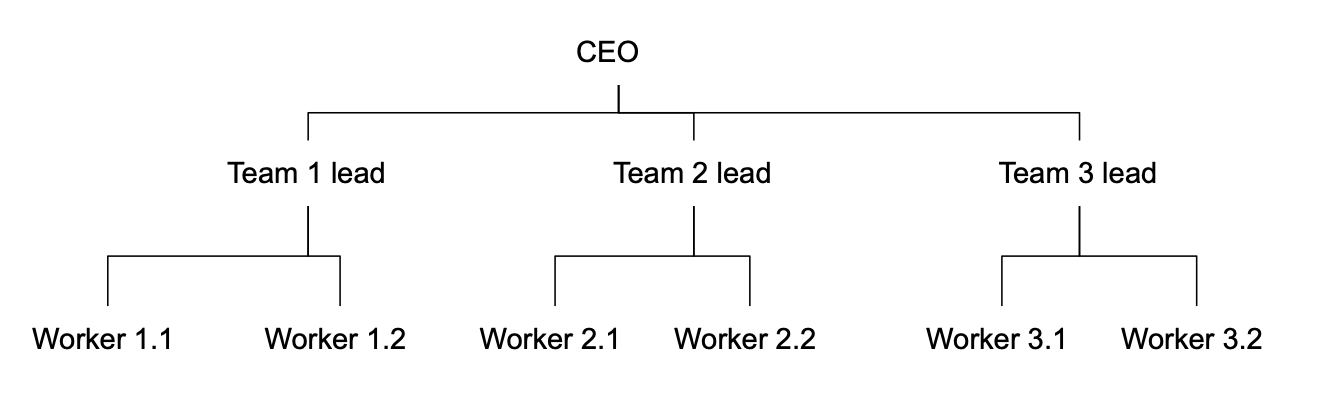
\includegraphics[width=1\textwidth]{images/org-chart-orientation-ceo-at-top.pdf}
\caption{Standard orientation. The role with the most responsibility and authority is at the top. Left-right ordering is intended to be irrelevant in this view, though left-to-right reading order emphasizes importance.}
\label{fig:org_chart_orientation_ceo-at-top}
\end{figure}

\begin{figure}
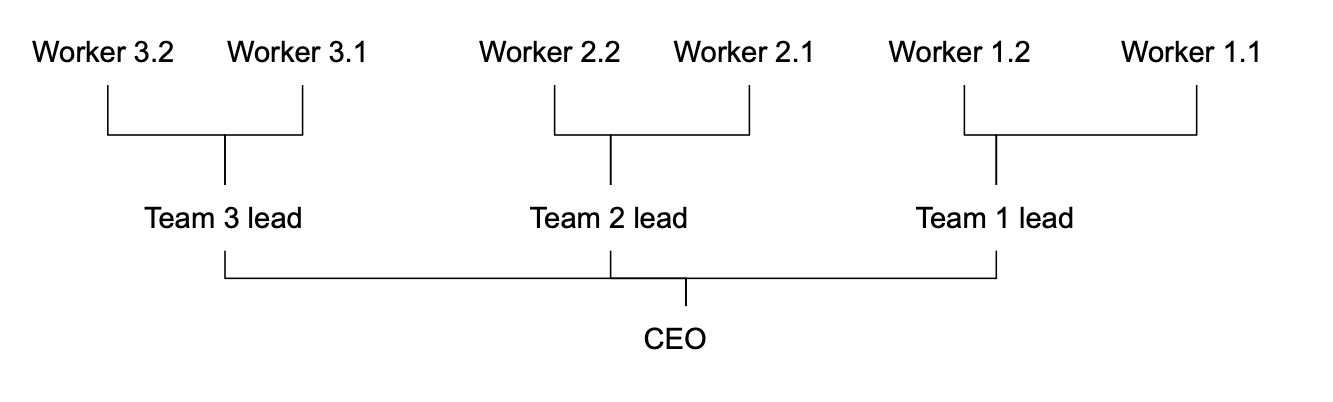
\includegraphics[width=1\textwidth]{images/org-chart-orientation-ceo-at-bottom.pdf}
\caption{Flipping the orientation presents a more realistic view of the CEO's responsibility. The crushing burden of servant leadership is clear. Left-right ordering is intended to be irrelevant in this view.}
\label{fig:org_chart_orientation_ceo-at-bottom}
\end{figure}

\begin{figure}
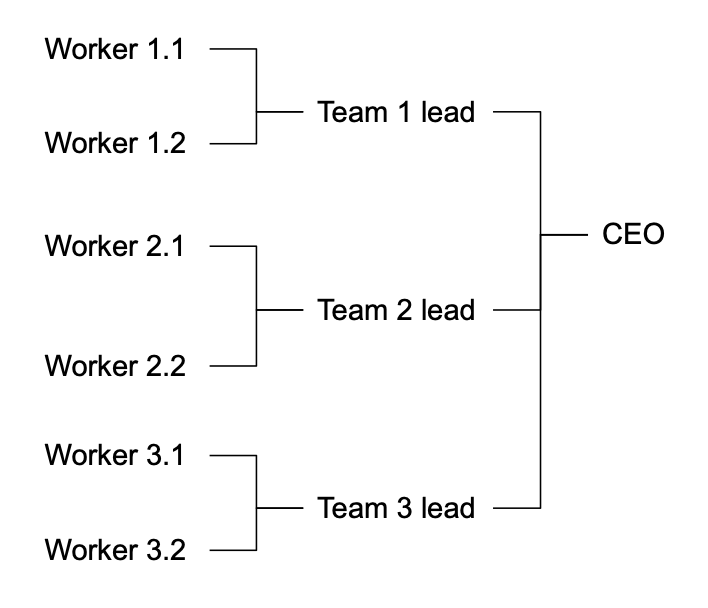
\includegraphics[width=0.8\textwidth]{images/org-chart-orientation-ceo-leads.pdf}
\caption{Conventionally time flows from left (old) to right (new), so in this graph the CEO leads the charge into the unknown. Is the CEO dragging workers forward, or are the workers pushing the CEO? The top-to-bottom order can be read as importance. }
\label{fig:org_chart_orientation_ceo-leads}
\end{figure}

\begin{figure}
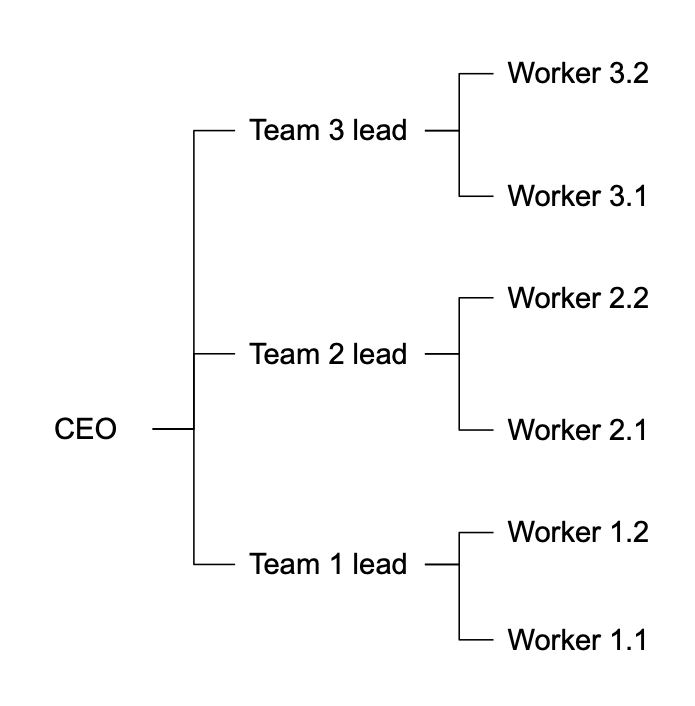
\includegraphics[width=0.8\textwidth]{images/org-chart-orientation-workers-lead.pdf}
\caption{The ``chariot view'' with the CEO in the chariot and the workers out front. Workers are in the future; the CEO is in the past operating on old information. As with Figure~\ref{fig:org_chart_orientation_ceo-leads}, top-to-bottom ordering can be read as importance. }
\label{fig:org_chart_orientation_ceo-follows}
\end{figure}

\begin{figure}
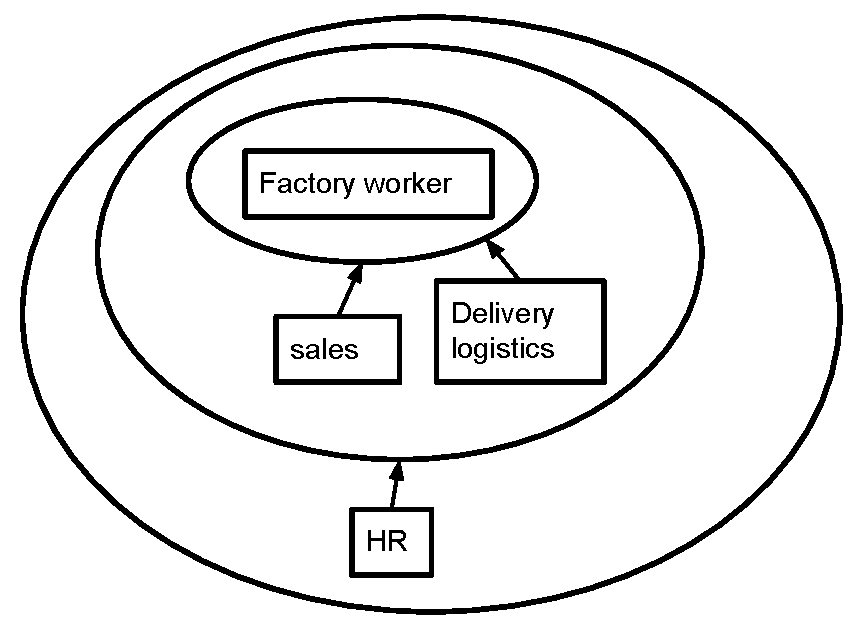
\includegraphics[width=0.8\textwidth]{images/org_chart_wedding_cake_dependencies_-_manufacturing.pdf}
\caption{An internal-customer-oriented view rather than a reporting-oriented view. The center of the bullseye is the team that generates the value that is the focus of the business or the organization.
The outer rings support teams that exist in the inner rings. The diagram is specific to an organization's domain. This visualization identifies which teams are the customers of which other teams in an organization.}
\label{fig:org_chart_wedding_cake_manufacturing}
\end{figure}



%extension of 
% \href{https://en.wikipedia.org/wiki/Conway\%27s_law}{Conway's law}: seating chart reflects org chart \clearpage
    \section{Learning from Failure\label{sec:learn-from-failure}}

This section on individual failure is separate from
%\ifsectionref
%section~\ref{sec:org-failure-and-success} on 
%\fi
\hyperref[sec:org-failure-and-success]{how an organization characterizes failure}\iftoggle{haspagenumbers}{ (see page~\pageref{sec:org-failure-and-success}).}{.}

\ \\

Making progress in a bureaucracy is not a linear sequence of steps. Ideally there is an ongoing cycle of trying something, not succeeding, and then applying what you learn towards the next try. This idealized ``\href{https://en.wikipedia.org/wiki/Fail-fast\%23Business}{fail-fast}'' 
\index{Wikipedia!\href{https://en.wikipedia.org/wiki/Fail-fast\%23Business}{fail-fast}}\iftoggle{WPinmargin}{\marginpar{$>$Wikipedia: Fail-fast}}{}
cycle does not occur naturally -- the participants have to either have intrinsic motivation or external incentives to make progress. Failing as a path for learning is justified after having exhausted less expensive alternative education opportunities like reading books, going to school, and talking with experts. 

The recognition of failure depends on a clear measurement. Do the participants know the measure, and can they make the measurement? Having a defined measure of failure and regularly making the measurement relies on having an understanding of the expectations for the situation. Expectations are assumptions about the future.

Assumptions about the future can be categorized as
\begin{itemize}
    \item Opinions. For example, the interpretation of policy. Policy interpretation can be bent or exceptions can be made. 
    \item Guesses; more formally interpolation -- ``Given multiple options, X seems most likely."
    \item Experience; more formally extrapolation -- ``Last time X happened, so next time ...''
\end{itemize}

Failure with respect to expectations implies thinking about the future so that you can measure your progress (or failure). That is a subset of planning. You can fail if you don't plan, and you can fail if you do plan. This does not indicate that planning is irrelevant. Plans can be overly detailed and prescriptive, or plans can be inadequately specified; both are unhelpful.

If your measurements indicate failure, this could be due to an invalid assumption (with a valid objective) or you may have selected a bad objective. Declaring failure means re-evaluating assumptions, resetting objectives, or giving up on the concept and doing something else.

\ \\

There are ways to avoid failing: by not setting an objective, or setting an objective that isn't measurable. You can avoid the appearance of failure by not telling anyone the objective. Extrinsic accountability for failure requires other people to have awareness. If these tactics are being employed, it may be because the person (or
%\ifsectionref
%, in section~\ref{sec:org-failure-and-success}, 
%\fi
\marginpar{See page~\pageref{sec:org-failure-and-success}.}
\hyperref[sec:org-failure-and-success]{the organization}) doesn't want to share how they've failed until they have a success. 

Understanding rationales like the failure avoidance mentality is critical if you want to avoid feeling baffled the first time you encounter it. By learning these bureaucratic anti-patterns, you can inoculate yourself emotionally and cognitively. You now have a chance to think ahead before encountering the explanation.

A counterargument when you hear that someone is avoiding failure is to explain that noticing failure is essential to improving. Detecting indicators of failure, addressing the cause, and then changing is the process of improvement. When someone wants to avoid failure, I don't understand how they expect to improve. 

 \clearpage
    \section{Success (and failure) in Your Organization\label{sec:org-failure-and-success}}

This section on how a team or organization conceptualizes failure is separate from %section~\ref{sec:learn-from-failure}
\hyperref[sec:learn-from-failure]{learning from failure} 
\marginpar{See page~\pageref{sec:learn-from-failure}.}  
as an individual bureaucrat. 

Understanding the ways your organization succeeds or fails matters to you because it affects how you are evaluated and how you feel about your work. Success and failure are measured against a quantitative objective. 


Bureaucratic organizations have varying definitions of success and failure because organizations are made up of individual bureaucrats with a multitude of motives and weak feedback mechanisms. There are a few macro-level patterns for organizations. Each pattern has a consequence on the individual bureaucrats operating within the organization. 

\ \\

A bureaucratic organization that provides infrastructure service (such as a public water utility, an electrical power company, or an organization's internal computer support) has a specific failure mode. When infrastructure is unavailable or degraded, that's a failure. Success means satisfactory operation at a minimal cost. An organization operating in this context is motivated to avoid failure. Success is merely a lack of failure. An effort to improve processes or otherwise innovate will face the inertia of a culture organized around avoiding failure. 

\ \\

A bureaucratic organization that claims ``wins'' but no failures (because either more or different work is needed) is difficult to be productive in when the successful outcome has ill-defined value. The success can be counted (number of wins), but the relative importance of the success is unclear.

Examples of win-focused organizations include law enforcement, research teams, and teams with a responsibility for innovation. 

For an organization focused on ``wins,'' funding depends on how convincing these success narratives are. This biases the organization to focus on investments most likely to get more funding. When the funding for an organization does not come from consumers of products or policies created by the organization, there is a disconnect. The ``wins'' may not be helpful to the consumer.


% NOT INCLUDED -- need an example to make this more concrete
%A team that works to improve the productivity of other teams may have neither successes nor failures. Money and time are invested with the hope that results are useful to someone at some future time. If the team didn't exist no one would be significantly affected.  \clearpage
    \section{Promotion\label{sec:promotion}}

Bureaucrats get promoted for a variety of reasons: due to their technical competence, a role needs to be filled, to motivate retention, or for their managerial ability.  Not being promoted can feel like a slight against any of those reasons. 

In this section, folk wisdom illustrates the frustration bureaucrats have with promotion. The purpose of you familiarizing yourself with these sentiments is to understand that the failures of promotion are not specific to the team you are on or the organization you are a member of. The deficiencies are generic to hierarchy. With this insight, you can choose a more emotionally-healthy response to the situation. Process Empathy is intended to produce emotional resilience based on an improved understanding of the situation you are in.

\subsection*{Folk Wisdom about Promotion}

The 
\href{https://en.wikipedia.org/wiki/Dilbert_principle}{Dilbert principle}
\index{Wikipedia!\href{https://en.wikipedia.org/wiki/Dilbert_principle}{Dilbert principle}}
\marginpar{$>>$ Folk Wisdom} 
\index{folk wisdom!\href{https://en.wikipedia.org/wiki/Dilbert_principle}{Dilbert principle}}
says organizations
``Systematically promote incompetent employees to management to get them out of the workflow.''
A similar-in-spirit observation is 
\href{https://en.wikipedia.org/wiki/Putt\%27s_Law_and_the_Successful_Technocrat}{Putt's Law}
\index{Wikipedia!\href{https://en.wikipedia.org/wiki/Putt\%27s_Law_and_the_Successful_Technocrat}{Putt's Law}}
\marginpar{$>>$ Folk Wisdom}
\index{folk wisdom!\href{https://en.wikipedia.org/wiki/Putt\%27s_Law_and_the_Successful_Technocrat}{Putt's Law}}
which says,
``\sout{Technology}[Bureaucracy] is dominated by two types of people, those who understand what they do not manage and those who manage what they do not understand."
Those two observations are post-hoc rationalizations for managers lacking management skills and lacking technical skills. 

For bureaucrats who don't seem effective in their role, try to determine whether there is a lack of training, lack of awareness, or lack of interest. Training can take the form of reading books or attending classes. Lack of awareness can be addressed with measurements of turnover rate and surveying team members. 




\href{https://en.wikipedia.org/wiki/Peter_principle}{Peter principle}~\cite{1970_Peter}:
\index{Wikipedia!\href{https://en.wikipedia.org/wiki/Peter_principle}{Peter principle}}
\marginpar{$>>$ Folk Wisdom} 
\index{folk wisdom!\href{https://en.wikipedia.org/wiki/Peter_principle}{Peter principle}}
``People in a hierarchy tend to rise to `a level of respective incompetence': employees are promoted based on their success in previous jobs until they reach a level at which they are no longer competent, as skills in one job do not necessarily translate to another.''
% https://graphthinking.blogspot.com/2021/03/a-tension-between-working-at-discount.html
This incompetence might manifest as recurring failure for a person in a role they are inadequate for. More likely, your incompetence will blind you to your failures.

To avoid falling victim to the Peter principle, do not seek promotion until you have a track record of performing at the next level. The downside is that you are working at a discounted rate since you are providing value beyond what is expected of your grade. (That's Dilemma~\ref{table:dilemma-personal-work-extra-or-work-as-expected}\iftoggle{haspagenumbers}{ on page~\pageref{table:dilemma-personal-work-extra-or-work-as-expected}.)}{.)} 


% https://graphthinking.blogspot.com/2021/04/notes-from-peter-principle-by-peter-and.html
The Peter principle has an element of truth, especially when a person starts a new role. It takes time to find your footing in a new job. However, you can learn their role and become competent. %Also, the Peter principle relies on the simplification of a single dimension of intelligence.  \href{https://en.wikipedia.org/wiki/Theory_of_multiple_intelligences}{Gardner's theory of multiple intelligences}.
%\index{Wikipedia!\href{https://en.wikipedia.org/wiki/Theory_of_multiple_intelligences}{Theory of multiple intelligences}}
%\iftoggle{WPinmargin}{\marginpar{$>$Wikipedia: Theory of multiple intelligences}}{}


\subsection*{Designing Incentives Determines Values}
Promotion is critical when designing incentives for behavior. Promotion is challenging to engineer because people a driven by various motives like money, status, and authority. 


Promotion typically focuses on the past success of a person. This de-emphasizes teamwork and lessons learned from failures. 
Promotion of a person (rather than the team) results in hero culture.


%Lowering the value of learning from failures increases risk aversion. 
The risk tolerance of a bureaucratic organization is driven in part by tensions in the promotion processes: an interest in success (more success is better) and avoidance of failure (organizations don't promote for failing). This imbalance can lead participants to seek ownership of efforts that are likely to succeed, to seek easier successes, and to steal credit for outcomes created by other people. 

%\subsection*{Promotion and Risk}

The promotion process within an organization is coupled to the idea of innovation, even if your promotion is at odds with taking risks. 

 \clearpage

    \section{Ideas for Innovation within a Bureaucracy\label{sec:innovation}}



As a bureaucrat in an organization, you will see deficiencies and challenges. You could ignore the issues, complain but not take action, work around (avoid) the issues, or try to improve your organization. This section focuses on the last option.

Sometimes the issue and the apparent fix seem straightforward. If the situation has persisted for a long time, consider why the conditions have remained as is. 
Instead of framing your idea with, ``Isn't it obvious that things would be better if ..." learn why what seems obvious doesn't happen. 
Learn the history. Talk to participants. If there is agreement that the situation is harmful, why has no one else tackled it? If previous attempts to innovate were tried and failed, why did they fail? What is novel about your innovation?

If you understand the conditions creating a challenge, and the history of why other approaches failed, and you have an innovative response, consider the stakeholders. 
Innovation is necessarily disruptive to incumbent processes and teams and social power. 
Do the incumbents benefit from the proposed innovation? Have they said they will benefit, or are you projecting their response? 
Innovation that benefits the organization but harms incumbents is less likely to succeed. 

In addition to the social hurdles, innovation requires taking risks (otherwise the effort is merely incremental improvement). Risk in an organization means losing time or resources, potential harm to reputation, legal consequences. 

Once you decide to innovate, and after you've learned the history and talked to participants, you have choices about how to innovate:
\begin{itemize}
\item Innovate while ignoring the bureaucracy. Your scope is limited to what you can accomplish alone. Integration is tough and causes frustration.
\item Fight to create a space free from bureaucracy to enable innovation. You've intentionally isolated innovators from resources present in the organization, and integration back into the org is now more challenging. 
\item Leverage existing hierarchy and processes. Can be frustrating to work with bureaucrats who are not as focused as you are.
\end{itemize}


A recap of the innovation lifecycle in a bureaucracy:
\begin{enumerate}
    \item You see problems and challenges in your environment. This manifests as complaints from both the people directly harmed and observers who see inefficiency.
    \item You share ideas for innovation and gets feedback. Build a coalition of people willing to fight for the idea on your behalf
\marginpar{[Tag] Actionable Advice}
\index{actionable advice}
    so that when you're not present, the idea is still proceeding towards implementation.  That puts the threshold at ``so important other people are willing to pause whatever they were working on and take up your cause.''
    \item Enacting these suggestions require either a change to existing processes or new processes or an investment of work. These changes may not succeed -- there's risk. Your idea could fail because it's not a good idea. It could also fail because someone doesn't like you, or the idea doesn't account for some dependency you weren't aware of, or it might conflict with other changes in progress.
    \item If you do decide to invest effort, the activity takes you away from your current work. Enacting the change might involve skills you don't have; learning those skills takes time. Carrying out the activity with new skills increases the likelihood of novice mistakes.
    \item If someone else enacts the idea they get the credit for having done the work.
    \item If the idea saves money or time, there's typically no monetary reward. Recognition and benefit to your reputation isn't required as part of the change process. 
\end{enumerate}

There are many barriers in that lifecycle. The problem has to be observable to someone willing to invest effort in change. That person has to build a coalition of stakeholders. If the person isn't negatively harmed, that person may also lack clear benefit from resolving inefficiency. 

\ \\

In addition to the work of enacting the change, there is an administrative overhead of documenting the reason for the change. 
Subjective decisions mean choices have to be defensible. 
The need for defensible justifications result in conservative decisions and risk aversion and a decrease of motive for innovation. 

\ \\

Don't bother buying new technology because there's a lot of risk and we already know how to use the existing technology. (Same applies to innovation with policies.)

The people in decision making positions in the hierarchy have more experience with existing technology and are therefore biased against novel technology. Also, getting burned a few times on innovation makes people more conservative.

With limited time and staff available within the organization, experienced decision makers are typically not on the bleeding edge of the \href{https://en.wikipedia.org/wiki/Gartner_hype_cycle}{hype cycle}.
\index{Wikipedia!\href{https://en.wikipedia.org/wiki/Gartner_hype_cycle}{hype cycle}}

\ \\

Bureaucrats, recognizing that bureaucracy stifles innovation, will occasionally invest in internal innovation efforts. Because innovation can come from unexpected sources, the process of innovation is opened to everyone. 

Incompetent people can innovate just as much as well-informed experts, but the output of inexperienced people is more likely to be disappointing, wasteful, or even harmful. 

\ \\

These barriers lead to external observers to conclude something like the following simplification:
\begin{quote}
Bureaucracy destroys initiative. There is little that bureaucrats hate more than innovation, especially innovation that produces better results than the old routines.
\marginpar{[Tag] Folk Wisdom}
\index{folk wisdom!bureaucracy destroys initiative}
Improvements always make those at the top of the heap look inept. Who enjoys appearing inept?\footnote{Frank Herbert's 1987 ``Heretics of Dune'', page 201}%, Penguin}
% https://www.azquotes.com/quote/453163
\end{quote}

 \clearpage
    \subsection*{Changing your Environment}

% https://quoteinvestigator.com/2017/05/23/culture-eats/
%\begin{quote}
%    Culture Eats Strategy for breakfast
%\end{quote}
%\href{https://en.wikipedia.org/wiki/Peter_Drucker}{Peter Drucker}

Changing the bureaucratic organization you are a member of is difficult. That applies regardless of your motive for change and the thing to be changed. Regardless of motive, there are tactics applicable to any change. 
The two major categories of change are 
\marginpar{See page~\pageref{sec:change-a-process}.}
\hyperref[sec:change-a-process]{processes} (e.g., technical solutions, changing policy)
%\ifsectionref
%described in section~\ref{sec:change-a-process} 
%\fi
and changing the \gls{culture} of the members of an organization.
\iftoggle{glossaryinmargin}{\marginpar{[Glossary]}}{}

\ \\

Culture is the set of norms that determine acceptable behavior for members of the organization. Norms come from the expectations of your fellow bureaucrats. Your coworkers can model desired behavior and inflict punishments for deviations from norms. The culture of the organization is practiced by members. 

% https://graphthinking.blogspot.com/2021/01/why-active-shaping-of-culture-is.html
The expectations of culture should be stated explicitly. If the explicitly stated norms are in conflict with what is experienced by the organization's members, the hypocrisy decimates trust. 

Besides modeling desired norms in the organization, there are a few more tactics you can take. 
\marginpar{$>>$ Actionable Advice}
\index{actionable advice}
You can reinforce examples of desired behavior with public praise and meaningful rewards. You have the ability to punish examples of undesirable norms. 

Altering cultural norms of a bureaucratic organization means altering member behavior, adjusting incentives to re-enforce the desired behavior, punishing undesirable behavior, and providing resources to make the intended outcomes easier. 

Although aspects of culture may be problematic, thinking of cultural change as problem-solving is not a useful framing. Bureaucrats don't solve problems; they address challenges. The word ``problem" implies a solution. The problem-solution framing is inaccurate in a bureaucracy since altering the situation merely introduces novel challenges. 
Even though you don't solve a challenge, you can still get a sense of emotional reward from having improved the situation. 

\ \\

Prior to investing effort in change, reflect on the emotional and career impact of your effort. Will the work bring you joy, or is your emotional reward tied to the outcome? If the outcome is the only source of reward, you'll either be disappointed in failure or you will be more conservative (intending to increase the likelihood of success). The work of creating positive change can be joyful: you can form relationships and focus on learning. 

One of the challenges of change in a bureaucratic organization is figuring out what is worth changing. There are many opportunities for improvement. Talk to stakeholders and enumerate their challenges.
\marginpar{$>>$ Actionable Advice}
\index{actionable advice}
From the myriad stories, identify recurring themes and root causes. Typically bureaucratic challenges intertwine technical, budget, staffing, historical context, personalities of participants, and organizational politics. 

Select an aspect that you have some competence in and allows for growth. If the challenge is big (many people involved, takes a long time, costs a lot), can it be broken down into incremental challenges? Distinguish wide-scale changes from local changes over which you have more influence.

Having surveyed challenges worth addressing and having picked an issue with a high return on investment, the guidance of
\href{https://en.wikipedia.org/wiki/G._K._Chesterton\%23Chesterton\%27s_fence}{Chesterton's fence} 
\index{Wikipedia!\href{https://en.wikipedia.org/wiki/G._K._Chesterton\%23Chesterton\%27s_fence}{Chesterton's fence}}
\marginpar{$>>$ Folk Wisdom}
\index{folk wisdom!\href{https://en.wikipedia.org/wiki/G._K._Chesterton\%23Chesterton\%27s_fence}{Chesterton's fence}}
is that you shouldn't change something until you understand why things are the way they are. Figuring out the history of an issue can be work when there is a lack of historical records.

Talking to stakeholders in the survey phase may yield tidbits of history. Why have previous efforts been rejected or not taken effect? Written documentation of the history should be augmented by oral folklore. 

If your idea has a novel justification for success, identify all possible methods of progress and then rank the tasks. If you can't do all the work, who can you collaborate with? Can you delegate to people with skills you lack, or will you have to gain new skills? 
If no one has the relevant skills, becoming the widely-acknowledged expert gains power. 


 \clearpage
    \subsection*{Creating Change in the Organization\label{sec:creating-change}}

If the organization you are in has no problems or challenges, this section can be skipped. For bureaucrats in organizations that do have issues, this part of the book provides points to ponder independent of the specific problem.

As a bureaucrat, you have unique insight on the challenges the organization faces, and you have unique leverage to alter the situation.  While you could proceed haphazardly, an effective bureaucrat has vision. The vision is a story of what-could-be. This vision can be broken out as goals: specific measurable outcomes. Each goal requires contingency plans for achieving the goal. Plans are marked milestones which indicate whether the plan is proceeding successfully. 

Perspectives to consider when assessing change include what the situation is, what the situation could be, and what the situation looks like for different stakeholders. Each person has different information, a different way of responding to issues, and shifting intents.

People who you depend on who have conflicting visions or no vision, confounding your ability to improve the organization. There are different views on whether something is actually a problem, distinct characterizations of an issue, and competing priorities.

A trade-off to consider is that having niche impact is easier than broad change (the \hyperref[table:dilemma-personal-scope-broad-vs-narrow]{Dilemma of Scope of Effect}). 
\marginpar{See page~\pageref{table:dilemma-personal-scope-broad-vs-narrow}.}
There's also a trade-off of the quick fix versus more robust solutions (the \hyperref[table:dilemma-personal-quick-methodical]{Dilemma of Speed and Accuracy}).


%Determine social/political/technical impediments. 

\index{list of tips!change within an organization}

\ \\
% https://graphthinking.blogspot.com/2018/08/potential-paths-when-faced-with.html
\textit{Suggestion}: Understand and empathize with the fear of change. \\
When faced with a challenge, the options are to take action or to not take action. If you take action, the options are failure, success, or iteration. 
The choice of no action is attractive if you are not suffering. Delay minimizes work, enables beneficial moves since the player can wait out other players, and there are other things to focus on.

Action incurs risk due to uncertainty and costs work to create change.

Fear of failure is justified if and only if the cost of the failure is greater than the value of lessons learned.

Fear of iteration is a fear that the process might be stopped prematurely -- before perfection.

\ \\
\textit{Suggestion}: Before starting a new effort, check to see whether this has been tackled before.
\marginpar{[Tag] Actionable Advice}
\index{actionable advice}
Learn the history of the problem. Why hasn't this been solved?

\ \\
\textit{Suggestion}: Query your first and second order social network.
\marginpar{[Tag] Actionable Advice}
\index{actionable advice}

\ \\
\textit{Suggestion}: Get feedback early before polishing.
\marginpar{[Tag] Actionable Advice} 
\index{actionable advice}

\ \\
\textit{Suggestion}: Advertise the result.

\ \\
\textit{Suggestion}: Hear criticism and respond.

\ \\
\textit{Suggestion}: Leverage both social networks and bureaucratic processes. 

\ \\
\textit{Suggestion}: Identify sources of power (hierarchical positions and titles, social influence, reputation and credibility, buzzphrases or popular paradigms) and leverage them.

\ \\
\textit{Suggestion}: Professional respect (for what the other person knows) and professional curiosity (for what you don't know) \\
Example: Getting approval from multiple overseers in different hierarchies is hard. Often different objectives and incentives.


\ \\
% https://graphthinking.blogspot.com/2016/01/methodology-for-people-acting-as.html
\textit{Suggestion}: Use social recommendations to name relevant individuals.\\
Leverage the trust already in an existing social network by starting with ``Person A recommended I talk to you about X."


\ \\
% https://graphthinking.blogspot.com/2016/01/methodology-for-people-acting-as.html
\textit{Suggestion}: Sit in on meetings, listen to topics, see who is talking, who is attending. After the meeting talk to individuals about the meeting. Set up one-on-one informal discussions. Keep the first conversation  brief - 10 or 15 minutes. Your body language should indicate engagement and interest. ``Who else would you recommend talking to?" is the last question in the first conversation.

\ \\
\textit{Suggestion}: Consensus doesn't mean everyone agrees on the problem, the remedy, or the approach, or who's taking the action. Consensus in a bureaucracy means people aren't going to resist the change. \clearpage
    % https://graphthinking.blogspot.com/2020/05/invisible-bureaucracy.html

\subsection*{Social and Bureaucratic interactions\label{sec:socializing}}

Change in a bureaucracy can apply to processes and people, but a more amorphous concept is changing the culture of a team or organization. What is meant by ``culture'' usually refers to norms -- the expectations of behavior that individuals hold to. That definition of culture is generic; what is meant within a bureaucratic context requires jargon for the specific expectations.

To evaluate expectations we start by introducing categories of interactions. 
Interactions among members of an organization are either a social interaction or a bureaucratic interaction. 

As examples of each of these,
\begin{itemize}
\item \textit{Social interaction example}: ``Did you see the game on TV last night? Our team really did well, right? I wanted to get tickets for the game but they were sold out."
\item \textit{Bureaucratic interaction example}: ``You'll need to get approval from Sue before presenting your idea to the board for their review. Then talk with Russ and get his thoughts about how to proceed."
\end{itemize}
Both social and bureaucratic interactions are vital to cohesion in an organization. 


Bureaucratic interaction can be broken into two subcategories: 
\gls{visible bureaucracy} 
\marginpar{[Glossary]}
(procedures and processes are written down and can be discovered by stakeholders) and 
\gls{invisible bureaucracy} 
\marginpar{[Glossary]}
(procedures and processes are known to some stakeholders and are conveyed verbally to some of the other stakeholders).

Invisible bureaucracy is akin to related topics outside the professional environment: invisible domestic work\footnote{cleaning your living space, raising children, caring for pets; see~\cite{1987_Daniels}} and invisible relationship work\footnote{consistent need to delegate, being curious without reciprocation}. The work associated with emotional cohesion, logistics, planning, scheduling, and communicating is hard to quantify so it does not get counted.


The relevance of this jargon is to break down the components of an organization's ``culture" experienced by participants.
When someone in the organization advocates for changing the culture, which expectations are they specifically referring to? Invisible bureaucracy is the hardest to alter because it is undocumented and not counted.
%The ratio of social relationship to visible bureaucracy to invisible bureaucracy is a characterization of the culture. There are norms associated with each of these three categories.

Processes default to invisible bureaucracy because creating and maintaining documentation requires work. Making the documentation discoverable requires work.
%, and because some processes are embarrassingly inefficient. 
To make invisible bureaucracy visible, document the work and enable other people to find the documentation.
 \clearpage % subsection
    \section{Measuring Bureaucratic Maturity}
% https://graphthinking.blogspot.com/2021/07/three-measures-of-bureaucratic-maturity.html

Bureaucratic maturity of bureaucrats in an organization can be broken into three stages of behavior: complaining (acknowledges an issue but doesn't seek to resolve), seeing opportunity (``what if we..."), and finally enacting 
\href{https://en.wikipedia.org/wiki/Nudge_theory}{nudges} (ways to alter behaviors) or altering incentives.
\index{Wikipedia!Nudge theory@\href{https://en.wikipedia.org/wiki/Nudge_theory}{Nudge theory}}\iftoggle{WPinmargin}{\marginpar{$>$Wikipedia: Nudge theory}}{}

The first and most widespread behavior is to see a problem and then complain about the situation. This indicates an awareness of the environment but no creativity regarding what to do about the problems.

The second, less common behavior, is to see a problem and recognize the situation as an opportunity. This requires creativity and reframing. 

The third behavior is to see a problem and then alter the situation toward a vision. Changes could be through either direct action or by influencing others. 


\ \\

An individual bureaucrat can show one or more of these behaviors. 
That is, being capable of the third behavior still allows the person to complain about other topics. 

There is not a specific amount of experience within the organization needed to arrive at any of these three paradigms. A holistic understanding of the system helps.

The ``vision" of the third behavior could be in the form of a long-term (temporally distant) outcome, or the vision could be of immediate multi-party cooperation.  \clearpage

  % person-to-person relations
\chapter{Working with other Bureaucrats\label{sec:working-with-other-bureaucrats}}
\iftoggle{showbacktotoc}{{\footnotesize Back to the \hyperref[sec:toc]{Main Table of Contents}}}{}

\iftoggle{showbacktotoc}{\ \\}{}

\iftoggle{showminitoc}{\minitoc}{}

You were hired to do a job. That job relies on technical skills you've accumulated through education and experience. Now you're a member of 
 the team. You'll need to interact with other bureaucrats for various reasons:
delegating tasks, asking for help, offering help, seeking input, and offering input.
%\begin{itemize}
%    \item Delegation of tasks.
%    \item Asking for help.
%    \item Seeking input.
%    \item Offering help.
%    \item Offering input.
%\end{itemize}
While that generic observation sounds reasonable, in practice you encounter significant friction in getting things done. 
% https://graphthinking.blogspot.com/2016/07/if-everyone-is-doing-right-then-why-are.html
If everyone participating in a process thinks they are doing the right thing, then why are there suboptimal outcomes? Potential reasons include
\begin{itemize}
    \item Each participant in the process may have a limited view of other parts of the process. Each person talks only to adjacent participants.
    \item Each participant typically has a limited scope of responsibility. They don't need to know everything. Specialization can improve efficiency and cause harm.
    \item Each participant typically has a limited scope of authority. Even if the person knows more than  their role, they lack control over other aspects of the process.
    \item Participants typically have insufficient time, resources, and expertise to enact improvements.
    \item Participants in the process may have a common goal but use different methods for addressing the challenges.
\end{itemize}
Those are all potential constraints; they don't exclude being effective or improving the process. 
You can learn what someone else's priorities are and why those are priorities. 

% https://graphthinking.blogspot.com/2021/10/why-i-dont-like-being-in-management-role.html
Solo work may be more emotionally rewarding due to fewer external constraints, but the cost is that task complexity and scope are limited to the skills of the individual. 


When you can't do everything yourself, you rely on your team and members of the broader organization. You can treat this loss of independence within the organization (\href{https://en.wikipedia.org/wiki/Deindividuation}{deindividuation}) 
\index{Wikipedia!\href{https://en.wikipedia.org/wiki/Deindividuation}{deindividuation}}\iftoggle{WPinmargin}{\marginpar{$>$Wikipedia: deindividuation}}{}
as either sublimation (and feel suffocated) or an extension of your capacity and abilities (and feel empowered).

Working with others allows you to occasionally accomplish complex results beyond your skills or your bandwidth despite  collaborators not being under your control. How? Through persuasion. 
The challenge of collaboration is to multiply productivity rather than merely sum the output of a set of individuals. 

Inside an organization, cooperation/coordination is not held together by internal contracts or even \href{https://en.wikipedia.org/wiki/Service-level_agreement}{service-level agreements}. 
\index{Wikipedia!\href{https://en.wikipedia.org/wiki/Service-level_agreement}{service-level agreements}}\iftoggle{WPinmargin}{\marginpar{$>$Wikipedia: Service-level agreements}}{}
What keeps the organization together is the force of will of participants. 


\subsection*{Your Value to Fellow Bureaucrats}

% https://graphthinking.blogspot.com/2017/05/presence-with-attention-time-alertness.html
When you engage fellow bureaucrats as part of a process, you are investing your attention in the relationship. Relationships take time, which is time not spent on other opportunities. In addition to your time (and theirs), the other two factors are your attention and alertness. To illustrate the relevance of those aspects, consider the following. I can talk to you for 15 minutes, but if your attention is directed toward your phone, then you're not fully engaged with me. If you are paying attention during the time we have together but haven't slept for 36 hours, your alertness may not be 100\%. 

When interacting with fellow bureaucrats, are you giving them your attention? Are you alert to their input? While engaging, determine if they are not attentive or alert. You can be curious and ask if deferring the interaction would allow them to give more of their attention. If you're not feeling alert, let the people you're interacting with know.


 \clearpage % chapter
    \section{Motives of Bureaucrats\label{sec:motivations}}

Learning the diverse motives of bureaucrats you depend upon is instructive for finding causes of delay or opposition. If you expect everyone to have the same motives as you, then you will be surprised by the friction created by diverse motives. 

Motivations of participants are rarely, ``How can I make the organization more successful?" or even, ``How can I sell or produce more product?" Usually, motivation is based on personal fulfillment in various manifestations. By learning the motives of each bureaucrat - what they value in terms of a \href{https://en.wikipedia.org/wiki/Utility}{utility function}
\index{Wikipedia!utility function@\href{https://en.wikipedia.org/wiki/Utility}{utility function}}
and how they perceive risk - then you can gather data relevant to the argument and frame the narrative more effectively.


Bureaucrats on the same team with similar skill sets have similar external incentives. However, their intrinsic motives may be different and result in distinct behaviors. Within an organization, bureaucrats differ due to their intrinsic motivations,  extrinsic incentives, and the  person's risk tolerance. These three factors combine into emergent phenomena, leading teams and organizations to act in ways no individual member would. The dissonance of how (personified) organizations behave confounds observers outside the bureaucracy. If you were to talk to each member, you could find a reason for that person's behavior. 


% see https://en.wikipedia.org/wiki/Social_influence

Each bureaucrat has a motive, even the bureaucrats who do nothing. Bureaucratic nihilism (showing up for your job but choosing to not provide value) is an option, but it is not without cost.
% https://graphthinking.blogspot.com/2020/02/there-is-no-idle-status-for-paid.html
In an organization where you are a paid bureaucrat, you are either actively working to improve the organization or your existence is parasitic to the organization. There is no ``idle" status for paid employees in an organization with limited resources.

Employees may choose to stop contributing value if they perceive that a lack of action will not harm their options. There is a perceived disconnect between their actions and the consequences for the organization. This is not pure nihilism, as the person still  benefits from showing up (usually a paycheck).

Rationalizing money as the cause for action is just one of many potential sources.
There are a variety of motivations and incentives for bureaucrats: 
stability (aka job security, the comfort of a routine),
money (current pay or future earnings), 
travel, 
problem-solving, 
status, 
exerting power or control, 
the credibility of being associated with the organization (if the organization has a positive reputation), 
logistical convenience (``the office is near where I live''), 
service to people the organization serves.


As an example incentive for a bureaucrat, I want to avoid being too efficient such that I eliminate the need for my job, 
\marginpar{$>>$ \href{https://en.wikipedia.org/wiki/Goldilocks_principle}{Goldilocks balance}}
while not so inefficient that the organization fails and I lose my job. Increasing the efficiency of bureaucracy is desirable for the organization and the outcomes, but can be harmful to the bureaucrat's career.


The consequence of diverse motives is that expecting bureaucratic organizations to be logical, fair, consistent, and efficient is unreasonable even when every participant wants those features. Each bureaucrat thinks, ``I am logical, fair, consistent, and efficient.'' Therefore each bureaucrat expects other bureaucrats to meet those same (unrealistic) standards. Next, anthropomorphize the team or organization and expect the group to meet those standards. 

Even if each bureaucrat were logical, fair, consistent, and efficient (they are not, and neither are you), each person has a different motivation. %Internal motivation depends on what you value in the sense of a
%\index{Wikipedia!\href{https://en.wikipedia.org/wiki/Utility}{utility}}
%\href{https://en.wikipedia.org/wiki/Utility}{utility}\iftoggle{WPinmargin}{\marginpar{$>$Wikipedia: Utility}}{}
%function.  
At the same time, each person wants to accomplish something using their skills.% and reference their own experiences. 
Compounding the confusion, each bureaucrat has to coordinate using communication that has latency, limited bandwidth, and isn't precise.

When viewed from the outside, an expectation that bureaucracy feels illogical, unfair, inconsistent, and inefficient is a useful baseline. From inside the bureaucracy, a baseline expectation is that every bureaucrat is driven by different motives and uses distinct ways to tackle challenges. Working against bureaucratic entropy (an ongoing investment) yields improvements even though perfection is inaccessible.


\ \\

% TRANSITION to tropes

The above discussion might leave you with the impression that individual bureaucrats are distinct. While that's true, with a sufficient number of different people there are recurring themes that are detectable. The next section identifies common tropes you might encounter. \clearpage
    \section{Bureaucratic Tropes\label{sec:tropes}}

Any sufficiently large organization will have a diverse group of bureaucrats. From that diversity certain tropes emerge.\footnote{J.~Duffy, personal communication, 2017.} The value of recognizing these recurring patterns is to leverage their strengths so that you and that person can be more effective. 


\begin{itemize}
    \item \textit{Trope}: \textbf{Excited intern or new employee}. \\
    \textit{What you can do}: Their enthusiasm can be channeled to take on challenges other bureaucrats are scared of taking on for political reasons. Their na\"ivet\'e 
    % https://en.wiktionary.org/wiki/na%C3%AFvet%C3%A9
    should be remedied by pairing them with a mentor who can explain the organization's history and specific challenges.
    
    \item \textit{Trope}: \textbf{Retired in place}. \\
    \textit{What you can do}: Recognizing this attitude allows you to temper your expectations about their productivity. 
    
    \item \textit{Trope}: \textbf{Font of institutional memory}. Likes to explain how the current situation relates to his experience ten years ago. \\
    \textit{What you can do}: You can benefit from talking to this person about historical processes and what has been tried before. 
    
    \item \textit{Trope}: \textbf{``Let them eat cake'' managers} who are removed from challenges and deny the problem is a problem. \\
    \textit{What you can do}: It is worth figuring out whether these managers don't care, or if they are busy fighting battles you are not exposed to.
    
    \item \textit{Trope}: \textbf{``Don't rock the boat''} people who tried changing the system, didn't succeed, and are emotionally beaten down such that they no longer try. \\
    \textit{What you can do}: These people are often creative and can be consulted before you tackle a challenge they have experience with. 
    
    \item \textit{Trope}: \textbf{The Patriot} is willing to sacrifice for the organization. \\
    \textit{What you can do}: Educate them that there are alternative ways to be effective in a bureaucracy.
    
    \item \textit{Trope}: \textbf{Mismatched} -- this person's skills and interests don't match their role, so they are despondent and frustrated. \\
    \textit{What you can do}: You can provide value to this person by networking with them and finding better opportunities.
    
    \item \textit{Trope}: \textbf{Friendly grouch} is friendly and helpful but unhappy in their job due to bureaucracy and other hurdles. \\
    \textit{What you can do}: Provide a copy of this book to increase their effectiveness and improve their spirits. They will be grateful to you, and the organization will benefit.
    
    \item \textit{Trope}: \textbf{Detail-oriented} -- you ask them what time it is and they'll tell you how to build a clock. \\
    \textit{What you can do}: You can serve as their ambassador to other members of the team or organization.  
\end{itemize}


% see related but not relevant
% https://blog.codinghorror.com/which-online-discussion-archetype-are-you/
The above personality tropes apply to individuals. If your team works on multiple projects, you may identify project tropes:
\begin{itemize}
    \item \textit{Trope}: \textbf{We've always done it this way}.\\
    \textit{Assessment}: The team is scared of change. The change may be known (and undesirable) or unknown. Change disrupts power.\\
    \textit{What you can do}: You can brainstorm with the team ways to improve incrementally. 

    \item \textit{Trope}: \textbf{Individual solutions to systemic challenges}.\\
    \textit{Assessment}: Demonstrating small wins helps build credibility. \\
    \textit{What you can do}: Plan to ramp up  complexity (towards the systemic challenges) and \hyperref[sec:reputation]{spend the earned reputation}.
\marginpar{See page~\pageref{sec:reputation}.}
\end{itemize}
Team tropes can emerge from either the top-down directives made by supervisors or by the collective (in)actions of team members.


\ \\

% TRANSITION to solving_problems

Tropes as labeled patterns of behavior can decrease surprise when you first encounter them and can help you develop constructive responses. 

The last set of tropes is on the topic of bureaucratic problems.  \clearpage
    \subsection*{How to Solve Problems}

%This list is somewhat in jest, somewhat as a source of bureaucratic patterns.

Not every bureaucrat responds to challenges the same way. Understanding the diversity of potential reactions (or inaction) before you encounter them decreases the surprise. 

% TODO: someone else at work wrote this. Get their permission
\begin{itemize}
    \item Solve the problem. This is the engineering approach.
    \item Solve a simpler problem. This is the Physics approach.
    \item Solve a more abstract problem. This is the Mathematical approach.
    \item Solve a different problem.
    \item Recognize and ignore the problem. 
    \item What problem?
    \item Assign someone else the problem.
    \item Redefine the problem so that it is already solved. ``That's not a problem, that's how it's supposed to work.''
    \item Apply for resources (staff, training, money) to solve the problem.
    \item Point to the problem as a justification for more resources.
    \item Give a talk about the problem.
    \item Write a paper about the problem.
    \item Teach a course on the problem.
    \item Talk to your therapist about the problem.
    \item Your manager declares the problem solved and gets a bonus.
    \item Reframe the problem as an opportunity. 
    \item Study the problem in the context of the broader system.
    \item Study the problem from other people's perspective.
    \item Explore the impact of the problem on the broader system.
    \item Develop a set of activities for role playing parts of the problem. 
    \item Solve part of the problem. Then another part.
    \item Research whether anyone else worked on the problem.
    \item Find other instances of the problem that were already solved.
    \item Find similar problems and identify the differences.
    \item Contract out the solution and select a bid.
    \item Explain why the problem does not need to be solved.
    \item Explain why the problem is beneficial. 
    \item Form a team and set a mission statement addressing the problem.
    \item Slow-roll the problem until you don't need to worry about the problem. 
\end{itemize}


Did you recognize any of those responses from your past experiences? 
\marginpar{[Tag] Reflect and Discuss}
Were any unexpected? \clearpage
    \section{Not My Job: Task Scope}

% https://graphthinking.blogspot.com/2021/05/not-my-job-task-scope-and-collaboration.html

If you ask someone for help on a task that benefits your team, that person might respond that the task is ``not my job" and explain that time spent on tasks like what you're asking for gets in the way of their progress. The emotionally engaging work is not that task.

This recurring pattern is sufficiently common that at least one domain has jargon for the concept.
`\href{https://www.urbandictionary.com/define.php?term=scut}{Scut}'\iftoggle{WPinmargin}{\marginpar{[Urbandictionary.com] scut}}{}
is  slang in the medical field for the non-clinical yet essential tasks that do not require a doctor's degree or expertise.
%This is different from 
Another label used for non-central tasks is administrivia (short for administrative tasks).
%as ``scut'' would include taking out trash. 

A mindset related to the ``not my job" view is the following.
``Once I realized someone else has the same problem, I stopped worrying about it.'' The separation of scope can be reasonable (no point in duplicating effort) but may cause harm (when there's no coordination). The ``not my job" refusal is merely about scope. 

The potential reasons for this reluctance to help include
\begin{itemize}
    \item Working on the task will not get them promoted.
    \item Their understanding of the scope of their job and their expertise does not include the task.
    \item The person doesn't know how to do the task and they don't want to learn.
\end{itemize}
In any case, progress as measured by the individual refusing to help is not aligned with the success of the organization. You can escalate the request up the chain of command to get a determination about whether the collaboration should happen.

\ \\

% TRANSITION

Asking for help and giving (or refusing to give) help is dependent on your reputation.
The next section addresses how you can manage your reputation in a bureaucratic context. \clearpage
    \section{Building, Managing, and Spending Reputation\label{sec:reputation}}

% distinct from
%Social Capital https://en.wikipedia.org/wiki/Social_capital
%Political Capital https://en.wikipedia.org/wiki/Political_capital


%How does an individual create and accumulate political capital? What does political capital mean for teams?

This section is about actions you can take to create a reputation. Even if you don't intentionally build a reputation, you still get one because you interact with other people. Also in this section: how to spend political capital -- both yours and that of your team. 

\subsection*{Relevance of Reputation in a Bureaucracy}

As a bureaucrat, you may want to be all things to all people. Since that is not feasible, you have to limit your scope and therefore disappoint some people. This same dynamic of a limited scope applies to the team you are on, and again to the organization the team is part of. The purpose of a bureaucratic team or bureaucratic organization is to manage a \gls{shared resource} for a constituency. The constituency will invariably be disappointed because access to the shared resource is limited. 

The good news is that you can influence how others perceive your limitations. Their perception of your value is shaped by your investment in relationships and by your creative negotiations with other bureaucrats. %, other teams, and other organizations shape . 

\subsection*{Definition of Reputation}

Your \gls{reputation} as a bureaucrat is what other people expect from you. \iftoggle{glossaryinmargin}{\marginpar{[Glossary]}}{}
\index{reputation}
Reputation is perception. What does that person think of you? Your team? Your organization? 
Reputation is set whenever and where ever you are observed, or artifacts are associated with you. 
What you wear matters to how you are perceived. When you show up alters your reputation. How your written communication is read alters perceptions. People are informed by your body posture in meetings. 

\subsection*{Reputation, Brand, Image}

There are multiple phrases that all refer to the same concept of being perceived and generating associated expectations. Individuals create (or get) a reputation; organizations have brands. A team of bureaucrats can have a reputation. 

\subsection*{Your Reputation matters}

Your reputation within the organization dramatically alters your effectiveness. People will let you do things (or prevent you from doing things) based on their expectations of you. 

Your reputation alters your influence. Whether other people turn to you for input depends on what they expect from you. How others perceive you impacts what you can accomplish and when people seek your help or input.

\subsection*{You can Manage your Reputation}

Managing reputation means acknowledging that your interaction with others is partially performative. This may feel disappointing if you want to be judged solely on your productivity or knowledge. 

Your success is limited if you focus exclusively on doing the work, and your success is limited if you focus exclusively on performative aspects. 
Neglecting to manage your reputation means you lose input to the stories others tell about you. Active management of your reputation requires engaging with people and generating evidence. 

Your reputation is dynamically changing based on your activities and communication. Your communication matters, and the stories other people tell about you matter.

\subsection*{Techniques for Building Reputational Capital}

Ideally, your reputation would be based on your technical skills, your ability to collaborate with other people, the strength of your network, and your creativity. None of those matters if the person you're engaging with doesn't know those things. 
You build your reputation by doing things that are useful contributions, are visible to other people, and are associated with you (or your team or organization). This positive association is what you are creating.

Because the definition of reputation is about expectations other people have about you, what you choose to work on matters. How you work on your tasks (creativity, enthusiasm, dedication), the artifacts produced, and your ability to communicate all shape your reputation. 

When building your reputation, you can work on multiple small wins or take larger risks on bigger bets. The bigger bets provide faster leverage of reputational capital as you have shown your worthiness and skill. 

The same concepts apply to teams of bureaucrats and bureaucratic organizations. Just as individuals compete for resources, teams compete for budget, staffing, and glory. How the team's budget and staffing are spent inform reputation. 

A specific technique for building a good reputation is 
\hyperref[sec:credit-others]{giving others credit}. 
%(section~\ref{sec:credit-others}).
\marginpar{$>>$ Actionable Advice}
\index{actionable advice}
This may seem counter-intuitive if you are focused on assignment of credit. What  matters is that other people observe you (whether directly or indirectly) giving credit. 

Similarly, another technique for building good reputation is offering to \hyperref[sec:take-blame]{take blame}.
%(section~\ref{sec:take-blame}).
\marginpar{$>>$ Actionable Advice}
\index{actionable advice}
Again, this can seem counter-intuitive since being blamed doesn't sound good. The value is in proclaiming your willingness to be blamed such that other people observe your offer. 

\subsection*{Using Good News (or Early News) to Increase Influence}

Rather than tell good news directly to a top-level decision-maker, first inform the person who influences the decision-maker.
\marginpar{$>>$ Actionable Advice}
\index{actionable advice}
You can tell the influencer the information does not need to be credited to yourself.

The benefits of this approach include
\begin{itemize}
    \item Improves the influencer's reputation with the decision-maker.
    \item The influencer can contextualize the information for the decision-maker.
    \item The influencer can leverage the information in ways you would not have.
    \item My reputation with the influencer is enhanced.
    \item You reaffirm the influencer's role and status.
    \item Influencers can be easier to access.
\end{itemize}

\subsection*{How to Spend Reputation}

Based on your reputation (what the other person expects), what trust does that person have?  You can then use that trust to do things that might not otherwise be feasible. You can spend your reputation to bend  rules. 

Reputation is not the only thing you as a bureaucrat can spend. Other examples include your time (up to your entire career), your ability to be a member of the team or organization, your self-respect, and your ability to be promoted or receive bonuses. At the level of the team and the organization, additional aspects to spend are  budget and  staff. Each of these (reputation, time, membership, budget, staffing) are potential investments. 
%Confusingly, the investments are not independent. 

When considering what to spend to build reputation, consider what boundaries you have. 
Things you might not want to spend include your integrity and your health (physical, mental, emotional). Similar boundaries apply at the team and organization levels -- trust in the team, the well-being of team members. 


Whenever you engage within your team, you are either actively spending or building your reputation within the team.
Whenever you are engaging with people from outside your team, you are either actively spending or building your team's reputation.
Because of that, spending reputation means taking risks that involve other people.

\ \\

Examples of spending reputation and not getting a return on the investment:
\begin{itemize}
    \item Ask for a favor and provide no value.
    \item Explore options that other people don't see as worthwhile and then there's no payoff.
    \item Produce nothing of value to the organization or other people.
    \item Talk with people outside your team and misrepresent the efforts of your team.
    \item Speak honestly about the faults of your team to people outside your team.
\end{itemize}




%Internal-to-the-org there is cultural norms. 
% https://graphthinking.blogspot.com/2021/01/why-active-shaping-of-culture-is.html


% https://graphthinking.blogspot.com/2018/05/my-evolving-view-on-role-of-my.html


% the following article is useless
% https://www.indeed.com/career-advice/career-development/build-a-reputation
% since it reduces to "be a good person"


% https://graphthinking.blogspot.com/2021/09/notes-from-class-on-being-politically.html


 \clearpage
    % https://graphthinking.blogspot.com/2021/07/patterns-anti-patterns-in-bureaucracy.html

% intra- and inter- team dynamics

\subsection*{Teams are Subdivisions of an Organization}

A flat organization (more employees per manager) means more people doing work instead of managing, but sufficiently large organizations are typically broken into teams to make coordination less chaotic. 

%TODO: \cite{2015_Katzenbach} (Wisdom of Teams book).

As a bureaucrat on a team, you might expect that there are structural ways to address challenges. 
In the context of altering teams, there are only a few options available: create a new team, merge teams, or dissolve a team. 

Not all changes have to be structural; there are choices to be made when operating within the existing hierarchy.
For a given set of teams, the lateral interactions are competitive or cooperative. Coordination is required (or conflict will occur) for money, staffing, and resources. Examples of resources include access to or control of data, computer equipment, hardware, floor space, prestige, and ownership of products.

The purpose of pointing out the variables that can be changed is that there aren't many. As a consequence, the importance of  relationships and effective communication is more significant. 

\subsection*{Roles of Management versus Leadership}

\index{mantra!management isn't leadership}
Teams include managers and leaders. Those roles are not necessarily filled by the same person. By clarifying the distinction, you can determine what to expect from various members of the hierarchy. A common mistake is to expect leadership from managers. 

A manager's role involves time management, task tracking, employee evaluations, promotion, pay, requesting resources for team members, and hiring. Sometimes the responsibilities of promotion, pay, and hiring are split into a supervisor role, leaving task tracking and time management to the project manager or product manager roles.

A leader's role focuses on coordinating vision and principles. The vision and principles do not have to originate from the leader -- other team members can contribute ideas. The leader's responsibility is primarily social consensus and aligning the goals of members. 
 % no clearpage here because the next input is a subsection
    \subsection*{Sources of Friction between Teams within an Organization}

Ideally there is a clear division of responsibilities among different teams. Having separate teams requires interaction among teams -- one team may depend on the output from another team. Coordination among the teams regarding the transfer of data, products, projects, or knowledge is critical to the smooth operation of the organization. Separation allows for de-duplication of work and easier transitions for work that spans teams. 

The division of  responsibilities between teams can become unclear because a team's scope tends to align with skills of the team members. One team may be responsible for an aspect of a task workflow, but if members of another team also have those skills (e.g., due to cross-training), the separation between responsibilities can be blurred. 
 

Another factor that leads to friction is the constraint that organizations have finite staffing, money, and time. Therefore, teams within the organization face a \href{https://en.wikipedia.org/wiki/Zero-sum_game}{zero-sum}
\index{Wikipedia!zero-sum game@\href{https://en.wikipedia.org/wiki/Zero-sum_game}{zero-sum game}}
distribution of resources -- more for one team means less for everyone else. While cooperation among teams would be efficient, competition is created in the allocation of resources.

As with coordination among individual bureaucrats, a source of friction for teams is the differences in perspective based on local conditions, having insufficient education or experience, different incentives, or different definitions of success. Ideally each team shares the organization's vision, but in practice local conditions influence decision-makers.

When trying to resolve friction between teams, there is an authority common to the teams due to the hierarchical structure of responsibilities. That person who, by position, is responsible for resolving conflict, lacks nuanced insight, doesn't have time to get involved in every challenge, and doesn't want to micromanage multiple teams. The resolution is often left to the respective teams. 

%\subsection*{Data Transfer }

%\marginpar{[Tag] Story Time}
\index{story time!data transfer}
%\begin{storytime}{Data Transfer}
\begin{mdframed}[frametitle={Data Transfer from one Team to Another},frametitlerule=true,frametitlealignment=\centering]
Two teams in an organization have a relationship, and each has data storage and data processing capability. Allen's team sends Bob's team data on a weekly basis. Because the teams were built for different purposes and at different times by different people, the data storage capabilities used by each team are not compatible. Members of Allen's team print all the records (usually about a hundred pages) and then delivers the paper documents to Bob's team. Members of Bob's team then retype all the information into the data storage used by Bob's team.

Recently the office went paperless. Now Allen's team sends Bob's team a set of PDF files. Member's of Bob's team type in the content from the PDFs into the database for Bob's team. This is deemed a win for efficiency -- no more printing of paper documents each week!

Why doesn't the organization common to both teams hire a data scientist to automate the recurring data transfer? Or train the current staff to learn to program a solution? Or create a third team that manages a common server?
Because the current staff skill set supports printing and typing (data entry). Training someone with a new skill set takes an investment of money, time, is an opportunity cost, and makes them a flight risk.
Hiring a data scientist is expensive. Whether the task is feasible is uncertain from the view of Bob and his manager (they both lack experience with the needed technology), and how long the task will take is uncertain. Even once they create a connection, then a person with the skill set to maintain it is needed. The cost of ongoing maintenance and implementation is unknown.

\end{mdframed}
%\end{storytime}
The choices for resolving this friction between teams is to either stick with the known working approach that is suboptimal and has a known cost, or take a risk with unknown potential improvement of unknown degree for an unknown capital and unknown ongoing cost.
And if that improvement works out, staff who were enacting the current solution would need to find new work or learn new skills.
 
    \clearpage
    \section{Intellectual Empathy\label{sec:intellectual-empathy}}

As a bureaucrat, you will work with people who are smarter on a specific topic than you are. That superior knowledge might come from experience or from formal education. 

The person with superior knowledge may be able to convey their knowledge to you, or they may struggle to. That struggle could be due to an inability to break down complex insights, or they don't recognize the mismatch between what they know and what you understand. 
This same scenario can be reversed -- you might be more knowledgeable on a given topic than some other bureaucrat you work with. In either situation, both parties have responsibilities of intellectual empathy. The more knowledgeable person needs to understand what they can build on when talking with the less knowledgeable person, and the less knowledgeable person has to be clear about what is making sense and what does not. 

I often start conversations with people who are new to me by asking about their professional background -- their education, past work experience, and other aspects that would allow me to build on their existing knowledge. This allows me to tailor the conversation to the gap of knowledge that exists when we are discussing a challenge. 

During a conversation you can monitor body language for reactions like a squint, a head tilt, an eyebrow raise or an eyebrow furrowed. Those are common reactions when information doesn't conform to what the listener expected. 

A more direct method is to ask about the other person's knowledge of the topic. The phrasing ``Do you know about (name of topic)?'' is less effective than ``What do you know about (name of topic)?'' Respondents might claim experience or knowledge of a topic, but probing for the difference between ``I've heard those words before'' versus ``I was part of a team that implemented (topic)'' versus ``I came up with the original idea for (topic)'' is helpful. 

Sometimes the person with less knowledge on a topic feels uncomfortable with indicating their confusion, or sometimes the person doesn't realize they are missing the main point. The more knowledgeable person can check in with the listener to confirm. ``What did you get from what I just talked about?'' is a better confirmation than ``You understood what I meant, right?'' The person with less knowledge can proactively check their knowledge by providing a read-back: ``Here's what I understood you to mean: ...'' These check-ins, regardless of who initiates, should be relatively frequent when exploring complex topics. 

Admitting ignorance can be intimidating and may feel like you risk losing the other person's respect. A gentler way of saying ``I'm lost'' is ``I was following up until the point where you described ...'' Intellectual empathy is the responsibility of both parties in a conversation.  \clearpage
    \section{Leveraging Expertise\label{sec:expertise}}


%**************************************
% Generic observations on Expertise
%**************************************

The definition of \gls{bureaucracy} is the management of shared resources. Besides tangible items like land and water and air, expertise is another shared resource. Finding people with expertise, vetting expertise, and deploying expertise are all critical skills for bureaucrats. 

Experts who accumulate knowledge and experience look for ways to apply their expertise. Finding the right decision makers and providing relevant context for decisions can feel satisfying when positive impacts are made. 


In the following two sections I describe both viewpoints: that of a bureaucrat seeking expert help, and that of an expert providing help. Bridging the cultural and knowledge gap in both directions is necessary for the success of an organization.

\subsection*{Non-experts seeking Experts}
%*******************************************************
% Advice for Bureaucrats collaborating with Experts
%*******************************************************

Before you seek expert help, your first instinct may be to try and proceed on your own. Or with help from a peer, or a trusted consultant. \textit{How hard could this be? Looks straightforward...}

A typical starting point for a challenging decision would be to collect data and then form a narrative based on that. Surprisingly, there are bureaucrats who take the opposite view: Don't measure things; if you do you'll be held accountable for them. 

Setting aside the avoidance of accountability for a moment, there is reasoning behind the intent to not measure.  \href{https://en.wikipedia.org/wiki/Goodhart\%27s_law}{Goodhart's law}
\marginpar{[Tag] Folk Wisdom}
\index{Wikipedia!\href{https://en.wikipedia.org/wiki/Goodhart\%27s_law}{Goodhart's law}}
\index{folk wisdom!\href{https://en.wikipedia.org/wiki/Goodhart\%27s_law}{Goodhart's law}}
%%%TODO\marginpar{[Wikipedia] Goodhart's law}
says that ``when a measure becomes a target, it ceases to be a good measure.'' While there are ways to minimize this (e.g., not telling people what you're measuring), what you invest in measuring should be proxies for what the organization values.

If you decide a challenge requires skills you don't have, anyone with those skills has more expertise than you. Expertise is relative. 

\subsubsection*{Finding Experts}

One reason you as a bureaucrat seek an expert is you don't have expertise yourself. (If your motivation is merely to seek an external scapegoat that can be blamed, then getting any expert that appears convincing will suffice.)

To find a relevantly qualified expert, you can triangulate. Seek guidance from your existing social network. Multiple referrals from independent parties are a positive indicator. 

Do people defer to the candidate because of the candidate's title or position in the hierarchy, the candidate's experience, or the candidate's knowledge of technical details?

Within an area of expertise there may be sub-disciplines that you are not familiar with. Don't be embarrassed to ask the expert you find what subfield they have experience in, and their evaluation of how well that aligns with the effort you're recruiting them for.

If you're tackling a complex challenge, you may need experts from different disciplines. This introduces added challenges of cross-discipline communication. 



%\begin{itemize}
%    \item When asked about the topic, does the candidate respond defensively (emotionally) or with an anecdote or with a direct answer (logical)?
    %\item Does the candidate know the history of the topic? The important people in the field? The history matters for understanding the evolution of mistakes and innovations of the topic.
 %   \item Does the candidate know who the stakeholders are for the current situation? 
%\end{itemize}


\subsubsection*{Communicating with Experts}
Once you find a candidate expert, you'll need to evaluate their expertise and the ability to collaborate. This is inherently difficult since you lack expertise you are seeking. 

When signaled solely by credentials, expertise is independent of experience. The expert may lack ability to communicate their knowledge with people outside their domain. A common barrier is use of jargon by experts.

Jargon can serve two purposes: to signal group membership (harmful to people outside the group); and to be more precise about a concept (desirable). An pseudo-expert may use jargon relevant to a topic but not be able to explain

Levels of expertise:
\begin{enumerate}
    \item Self-designated expert is unfamiliar with domain-specific jargon.
    \item Pseudo-expert can use jargon in discussion but cannot expand the definition or provide analogs.
    \item Pseudo-expert has memorized definitions and has analogies but doesn't grasp underlying relations and principles.
    \item Expert can map situation-of-interest to underlying relations and principles, then use that mapping to remedy the issue (or explain why a fix is infeasible). The result works and the solution wasn't obvious to non-experts.
\end{enumerate}


Experts are cautious to include caveats and limitations.

Does the candidate use the relevant jargon for the topic?

Does the candidate use the jargon for the topic in the right way?
    
Can the candidate explain the topic with minimal use of jargon?

\ \\

\subsubsection*{What to use an Expert For}

Translation process is necessary from ``here's what's known in general" + ``situation specific facts" to ``plan of (in)action" and what's realistic with what confidence. 

Experts straying outside their expertise are dangerous because the boundary may not be clear to the audience.


%***************************************************
% Advice for Experts collaborating with Bureaucrats
%***************************************************
\subsection*{For Experts looking to help non-expert decision makers}


\subsubsection*{Finding the relevant person to provide advice to}



\subsubsection*{How to talk with non-experts}

Coherence of data can lead to increased confidence about the results.
Having less data may be more coherent. 

More data is likely to be less consistent and therefore lowers confidence.

\ \\

Non-experts think and speak less precisely.

You will need to simplify in the sense of applying to the relevant decisions - funding, staffing, planning.

\ \\

% https://graphthinking.blogspot.com/2012/05/notes-on-consulting-experience.html
You, the expert, may not win any debates based on number of years of experience. Some audiences may have many years in the field. However, expertise (rather than experience) is what they can benefit from. 

Identify which party (you, the expert, or the non-expert audience) has broader diversity of situations.

Respect and account for the expertise of the audience (especially when they work in a different field). Acknowledge your  limits.

Don't rely completely on expertise as a single dimensional relation. Find ways to relate personally to audience members. They will need to build trust in you personally.

Facilitate the audience setting the goals. They should be able to identify how success is defined.

Identify strengths your audience has and build on those.

You don't have to teach a group all-at-once. One-on-one teaching is more customizable, and the audience may feel less worried about asking dumb questions.

Once you've taught more than one person, they can help each other translate the skill. 



\subsubsection*{Advice for Experts}

Being the sole subject matter expert in an organization can feel isolating. You are constantly educating others but the stakeholders are not expected to become your peers. Typically stakeholders want to know just enough to make a decision. 

You are unable to ask someone smarter than you. Membership in professional organizations.

Cultivate your replacement.  \clearpage
    \section{Does Anyone Want to Volunteer?}

Bureaucracy relies on coordination to facilitate the management of shared resources. In the course of coordination, new tasks arise that have no one clear person responsible. The word volunteer has two meanings in this setting: contributing without seeking financial gain, and choosing to contribute of your own free will. 

% https://graphthinking.blogspot.com/2020/06/what-to-ask-instead-of-does-anyone-want.html

When the facilitator of a meeting asks the group, ``Does anyone want to volunteer for this task?" the question is often met with silence. No one wants extra work that does not help them, even if there is benefit to the team or organization. 
The lack of response is the \href{https://en.wikipedia.org/wiki/Tragedy_of_the_commons}{Tragedy of the commons}, 
\index{Wikipedia!\href{https://en.wikipedia.org/wiki/Tragedy_of_the_commons}{Tragedy of the commons}}
but in an anticipatory sense.
Instead of asking this poorly-framed question, the facilitator can get higher engagement with the following tactics:
\begin{enumerate}
    \item Ask each person in the meeting whether they are attending to passively observe or to participate.
    \item Ask each person willing to participate how much time they are able to invest. Responses could be zero hours, one hour (non-recurring), one hour per month, or something else.
    \item Ask each person what their goals in the interaction are. It is usually generic (``I want the group to succeed.") but it can be narrow, in which case that gives you something to focus on.
    \item Ask each person what they are good at and what skills they have. Are they good with personal interaction? Writing? Computers? Coordinating? Logistics? Fundraising? Making phone calls?
    \item From the inventory of tasks, are there any that fit both the skills and time? Can the task be scoped to fit the time? If there are multiple candidate tasks for a volunteer, let them pick the task. (If no existing task aligns with their skills, do not create work to be assigned.)
    \item If there are other people working on the same task, put the volunteer in contact with the other people.
    \item Give the volunteer a deadline for the task. Your deadline should not be arbitrary -- it should be based on the task dependencies. 
    \item Confirm that the volunteer is willing to commit the time to complete the tasks by the deadline.
    \item Schedule a check-in with the volunteer before the task deadline to review progress.
    \item To create accountability among multiple volunteers, hold a group review to explain how each participant's work contributes to the goals and how work done by one person enables the next task done by someone else. (Enumerate the dependency graph; include deadlines.)
\end{enumerate}

As the facilitator looking to designate tasks to participants, the above tactics align the work with the skills of contributors. 

As a contributor, your obligations to the team are knowing how much time you have to contribute and being clear about the relative priorities of tasks. Explaining that the new task is lower priority than all your other obligations is a valid response. Your responsibility is to negotiate with the person looking to assign new work and the people who depend on the results of your current tasks.  \clearpage

\chapter{Communication within a Bureaucracy\label{sec:communication-within-bureaucracy}}
\chaptermark{Communication}

\iftoggle{showbacktotoc}{{\footnotesize Back to the \hyperref[sec:toc]{Main Table of Contents}}}{}
\iftoggle{showminitoc}{\minitoc}{}


\section[Communication is Critical for Bureaucracy]{Communication is Critical for Bureaucracy\label{sec:critical-communication}\iftoggle{shortsectiontitle}{\sectionmark{Communication is Critical}}{}}
\iftoggle{shortsectiontitle}{\sectionmark{Communication is Critical}}{}

% LONG1 shows up in the TOC
% LONG2 is the section title

\iftoggle{glossaryinmargin}{\marginpar{[Glossary]}}{}
\iftoggle{glossarysubstitutionworks}{\Gls{decentralized bureaucracy}}{Decentralized bureaucracy}
relies on distributed knowledge and distributed decision-making. Distributed decision-making relies on effective communication. Bureaucrats communicate by writing and speaking; both methods convey incomplete information and are imprecise. The inability to communicate  comprehensively and precisely  means iteration is helpful when establishing a shared mental model of the situation and plan.


The dependence on iterative interactions means relationships matter for communication. 
\href{https://en.wikipedia.org/wiki/Metcalfe\%27s_law}{Metcalfe's law} 
\index{Wikipedia!Metcalfe's law@\href{https://en.wikipedia.org/wiki/Metcalfe\%27s_law}{Metcalfe's law}}
says
\marginpar{$>>$ Folk Wisdom}%
\index{folk wisdom!Metcalfe's law@\href{https://en.wikipedia.org/wiki/Metcalfe\%27s_law}{Metcalfe's law}}%
the value of an organization is proportional to the square of the number of people interacting in the organization. A team of 5 people is not just the aggregated skills of five individuals -- there's the synergy arising from ten bilateral relationships. Broadening your network of collaborators increases your potential effectiveness and, symmetrically, the reach of your fellow bureaucrats. 

% https://graphthinking.blogspot.com/2018/08/confusion-leads-to-confusion.html
Suppose that you don't invest in relationships with your fellow bureaucrats. Then you'll be less likely to know what is happening in your organization, and you won't understand why certain decisions were made. Your confusion might lead you to focus on your interests since that is what you have some control over and insight into. Being selfish doesn't leverage the potential synergy of collaboration, but at least you look busy. 

The analysis above applies to each person in the bureaucratic organization.
% A Nash equilibrium?
The consequence is that the organization's goals are not achieved when bureaucrats act independently. 
There is a way out of this: broadcast your intent to other people, be transparent with decisions, and share the results of your activities. That decreases the confusion other people may have about your actions and can improve everyone's effectiveness. You can make yourself and the organization more effective even when your investment in communication is not reciprocated.

\ \\

Information within a bureaucracy shapes the relationships among bureaucrats. You have a choice: you can decide to not share information, you can be transparent, or you can be vulnerable.  
Not sharing information can harm or protect relationships. 
Being transparent conveys ``here's what is happening." Being vulnerable expands transparency to explain ``here's why that's happening or what might happen."
Each of those options informs how your coworkers, peers, management, and team members interpret their perception of your intent. Your communication shapes your \hyperref[sec:reputation]{reputation}.
\marginpar{See page~\pageref{sec:reputation}.}


Another way communication alters bureaucratic organizations is when actions informed by locally available information produce \hyperref[sec:failure-to-comm]{suboptimal results for participants}, 
\marginpar{See page~\pageref{sec:failure-to-comm}.}%
as illustrated by the
\href{https://en.wikipedia.org/wiki/Prisoner\%27s\_dilemma}{Prisoner's dilemma}. 
\index{Wikipedia!Prisoner's dilemma@\href{https://en.wikipedia.org/wiki/Prisoner\%27s\_dilemma}{Prisoner's dilemma}} 

\begin{mdframed}[frametitle={Prisoner's Dilemma},frametitlerule=true,frametitlealignment=\centering]
(The \gls{Prisoner's dilemma} describes the following scenario. Two people suspected of a crime are held by police. The suspects are not allowed to communicate with each other. The suspects can either both remain silent (and be jailed for 1 year), one testifies against the other (in which case the silent person goes to jail for 3 years), or both testify and each goes to jail for 2 years.

Each suspect would select the testimony (resulting in betrayal) to minimize their imprisonment even though there's a better option of remaining silent since each suspect cannot predict the behavior of the other person. 
\label{prisoners_dilemma_explanation}
\end{mdframed}

As with suspects in the Prisoner's Dilemma scenario, bureaucrats rarely have access to the holistic view of their organization. Bureaucrats have a narrow view of their team and interfaces to adjacent teams.
The concept of ``locally available information'' applies to communication among bureaucrats that facilitates delegation of work, allocation of resources, relationship creation/maintenance, and carrying out processes. 

If having a holistic view yields better results, why not just do that instead of relying on local information? Each bureaucrat benefits from gathering information that shapes their actions, but communication has a cost: time spent building and verifying consensus delays action. You get fewer things done when you spend time talking with people. That trade-off of not being able to do everything well is called an 
\href{https://en.wikipedia.org/wiki/Opportunity_cost}{opportunity cost}.
\index{Wikipedia!opportunity cost@\href{https://en.wikipedia.org/wiki/Opportunity_cost}{opportunity cost}}\iftoggle{WPinmargin}{\marginpar{$>$Wikipedia: opportunity cost}}{}

% https://graphthinking.blogspot.com/2021/09/why-is-everything-so-hard-in-large.html


% TRANSITION to communication_reflects_thinking

\ \\

The explanations above show that communication is critical for bureaucracy and essential for being an effective bureaucrat. Communication occurs between two or more people, but before getting to that you need to improve your \href{https://en.wikipedia.org/wiki/Intrapersonal_communication}{inner monologue}. 
\index{Wikipedia!intrapersonal communication@\href{https://en.wikipedia.org/wiki/Intrapersonal_communication}{intrapersonal communication}}
\iftoggle{WPinmargin}{\marginpar{$>$Wikipedia: Intrapersonal communication}}{} \clearpage % chapter
    \section[Communication Reflects Your Thinking]{Communication Reflects and Shapes Your Thinking\iftoggle{shortsectiontitle}{\sectionmark{Communication and Your Thinking}}{}}
\iftoggle{shortsectiontitle}{\sectionmark{Communication and Your Thinking}}{}

% LONG1 shows up in the TOC
% LONG2 is the section title


Before you talk to another person, you have an internal dialog about how to interpret events and what you think will happen in the future. Your inner monologue shapes your expectations and your actions. When you talk with fellow bureaucrats, you're sharing some of your thoughts and allowing their thoughts to shape your contemplation. 

As a bureaucrat, you might have a few complaints you've thought about regarding your team or organization. Complaining about bureaucracy is a common way for bureaucrats to bond. Complaints occasionally lead to insights, but that's typically not the goal. 

By changing how you think about the challenges you face, you can alter your perception and your reputation. As an example of this change, can you turn complaints into impact statements? 
\marginpar{Actionable Advice}%
\index{actionable advice}%
The following examples show how to spin a negative experience. Providing a solution isn't required in this exercise. 

\ \\
\textit{Negative observation}: ``Logging into my computer takes a long time.''\\
\textit{Positive statement with explanation of impact}: ``If I were able to log into my computer more quickly, then I could do more tasks.''

\ \\
\textit{Negative observation}: ``I need support from a team that doesn't offer a way to track the status of my request.''\\
\textit{Positive statement with explanation of impact}: ``If the service team I need support from offered a way to track requests, then I would be able to know the status of my request.''

\ \\
\textit{Negative observation}: ``When I submit a support request to the team, I don't have visibility on the status of the request.''\\
\textit{Positive statement with explanation of impact}: ``If the service team I need support from offered visibility into their tracking of tasks, then I could proceed with other tasks knowing my request wasn't lost.''

\ \\
Sharing negativity is a way of commiserating, but it doesn't indicate to other people that you're adding value.  
When you notice a complaint, can you frame it as describing why the issue matters? 

\ \\

Another framing that harms your thinking and how you communicate is the use of generalizations. Personifying other teams and organizations is a simpler-to-understand and simpler-to-describe model, though the simplification is often incorrect. 

Here's a progression that shows how to transform generalizations into action: 
\marginpar{Actionable Advice}%
\index{actionable advice}%
\begin{enumerate}
    \item This organization does not like blueberry pie.
    \item No one in this organization likes blueberry pie.
    \item I don't know of anyone in the organization who likes blueberry pie.
    \item I like blueberry pie. How would I find someone else in the organization who wants blueberry pie?
\end{enumerate}
The first statement personifies the organization. Organizations cannot like or dislike tangible items, so that statement is meaningless. The second statement is slightly more precise (each person can have likes and dislikes) though still a generalization and therefore likely inaccurate. Did you confirm with every member of the organization that they do not like blueberry pie? The source of the generalization might be your lack of relationships with every member of the organization. That leads to the fourth statement which is correct, precise, and curious. 

\ \\

Now that you've reflected on how your internal dialog alters your perceptions and actions, the next section describes how communication goes wrong. \clearpage % subsection
    \section{Failure to Communicate\label{sec:failure-to-comm}}

Communication is critical in bureaucracy because bureaucracy is a system of distributed knowledge and distributed decision-making. When less effective communication occurs, individual bureaucrats are less able to rely on the knowledge of other experts, and they have to make decisions with less consensus. 

This section on failure outlines how ineffective communication happens. Identifying generic sources of difficulty is intended to help you distinguish what is common in bureaucratic organizations versus what is specific to the people you collaborate with. 


\ \\

Sometimes failure to communicate is caused by too much ineffective communication. 
You can get overwhelmed when there is a lot of communication happening (whether from too many sources or too much content).
Feeling saturated with meetings, emails, phone calls, and other coordination may stem from ineffective communication. 
Communication that is incorrect, imprecise, redundant, and insufficient can be improved. 
% https://graphthinking.blogspot.com/2016/04/impact-of-communication-on-negotiation.html
Improvement in communication effectiveness is more than just a time saver --
poor communication yields poor negotiation. When negotiations are not going well,  the interaction defaults to an emotional struggle of willpower. 


\subsection*{Why written communication does not happen\label{sec:written-comm-does-not-happen}}
If you can identify specific causes of why communication isn't happening, then you can intervene and address the concerns others may have. The following list is a set of common reasons that you can remedy by developing a workaround or by discussing explicitly. 
\begin{itemize}
    \item Too many reports, emails, and messages to read and process and respond to. Bureaucrats feel emotionally and cognitively overwhelmed.
\item The receiving bureaucrat may read slowly.
\item The bureaucrat-as-author may type slowly, or their handwriting is poor.
\item Potential participants fear imperfect communication. What if the email is incomplete or inaccurate or ambiguous?
\item The bureaucrat views written communication as ``official" or ``plan of record'' and feels uncomfortable brainstorming or creating contingency plans.
\item The bureaucrat wants to avoid accountability for their statements.
\item The bureaucrat may not be confident in their writing ability -- spelling, grammar, sentence composition, structuring content. \footnote{For tips on writing, see page~\pageref{sec:resources-for-writing}.}
\end{itemize}
Once you can identify why written communication is not happening, you can work with the other people involved to develop creative solutions. 

Another source of challenge for written communication is the latency of asynchronous interactions. By labeling distinct types of delay, you are better equipped to respond when the issue arises. 

\subsection*{Slowing Communication\label{sec:slowing-communication}}

In an ideal scenario there would be no delay associated with communication -- you would get the information you need when you need it. In practice, there are various causes for why your progress is blocked when you depend on other people. 

Tactics that delay communication within a bureaucratic organization are stonewalling, slow-rolling, bikeshedding, and red herrings. By learning these concepts you will be better able to identify and then respond to their use.

\index{responsiveness!stonewalling}
\iftoggle{glossaryinmargin}{\marginpar{[Glossary]}}{}
\iftoggle{glossarysubstitutionworks}{\Gls{stonewalling}}{Stonewalling} 
is when the recipient of a request or question  doesn't reply. There are \hyperref[sec:email-responsiveness]{legitimate reasons for the lack of response}\iftoggle{haspagenumbers}{; see page~\pageref{sec:email-responsiveness}.}{.}

The person may be busy and didn't see your message, or they did see your message but didn't have a chance to reply yet because a response to you is lower priority than other tasks they have. You cannot differentiate those reasonable causes from when the recipient doesn't want to enable you to proceed. They may disagree with your objective and see silence as \href{https://en.wikipedia.org/wiki/Passive-aggressive_behavior}{less confrontational}
\index{Wikipedia!passive-aggressive behavior@\href{https://en.wikipedia.org/wiki/Passive-aggressive_behavior}{passive-aggressive behavior}}\iftoggle{WPinmargin}{\marginpar{$>$Wikipedia: Passive-aggressive behavior}}{}
than explicit rejection. 

One way of circumventing stonewalling is to ask if the respondent is opposed to your idea. 
\marginpar{$>>$ Actionable Advice} 
\index{actionable advice}
Then a lack of response indicates no opposition. This tactic applies if you are confident the recipient will read or hear the message.

An unintentional source of stonewalling is when you ask on the wrong channel. Sending an email may result in what appears to be stonewalling if the person relies on chat messages or the phone. The solution for this 
\marginpar{$>>$ Actionable Advice} 
\index{actionable advice}
is feasible, but action is required by the person who doesn't respond. The person who only uses certain channels should explicitly indicate that. An automatic out-of-office email that says, ``Contact me by phone'' tells the sender the \hyperref[sec:communication-preferences]{preferred channel}. 
\marginpar{See page~\pageref{sec:communication-preferences}.}

From the view of the person doing the stonewalling, if you need time to think or gather information before responding, 
\marginpar{$>>$ Actionable Advice} 
\index{actionable advice}
tell the person who sent a request that you acknowledge their message and will follow up in more detail later (with a specific timeline). While better than no response, this leads to the next challenge.

\index{responsiveness!slow-rolling}
\iftoggle{glossaryinmargin}{\marginpar{[Glossary]}}{}
\iftoggle{glossarysubstitutionworks}{\Gls{slow-rolling}}{Slow-rolling} 
is when you get a response to your request or question, but the response isn't helpful. Progress is delayed because you have to iterate to get an answer. There are valid reasons for a slow-roll and there are uncool reasons for a slow-roll response. Perhaps the person wants to acknowledge your request but doesn't currently have time to provide a full explanation. The person may need to gather more information for the complete response. Or the person is \href{https://en.wikipedia.org/wiki/Passive-aggressive_behavior}{passive-aggressive}
\index{Wikipedia!passive-aggressive behavior@\href{https://en.wikipedia.org/wiki/Passive-aggressive_behavior}{passive-aggressive behavior}}\iftoggle{WPinmargin}{\marginpar{$>$Wikipedia: Passive-aggressive behavior}}{}
and may understand your question but does not want to enable your progress. 

The reason for a slow-roll should be made explicit by the respondent, 
\marginpar{$>>$ Actionable Advice}
\index{actionable advice}
and a timeline for a complete response is helpful. 


\label{concept:bikeshedding}
\index{responsiveness!bikeshedding}
\iftoggle{glossaryinmargin}{\marginpar{[Glossary]}}{}
\iftoggle{glossarysubstitutionworks}{\Gls{bikeshedding}}{Bikeshedding} 
is when the recipient of a question or request 
\href{https://en.wikipedia.org/wiki/Law_of_triviality}{focuses on unimportant details relative to the primary topic}. 
\index{Wikipedia!Law of Triviality@\href{https://en.wikipedia.org/wiki/Law_of_triviality}{Law of Triviality}}\iftoggle{WPinmargin}{\marginpar{$>$Wikipedia: Law of Triviality]}}{}
Whether this behavior is intentional or not, the best response is to refocus the conversation on the core issue. The amount of time allocated for various topics should be proportional to their consequence. 

\index{responsiveness!red herring}
A \gls{red herring}\iftoggle{glossaryinmargin}{\marginpar{[Glossary]}}{}
response is misleading, whether intentional or not. The respondent provides what looks like a reasonable answer but results in unproductive work. Occasionally there is a coincidental benefit of discovering something unexpected, but that wasn't the respondent's intent. 


Even though bikeshedding and a red herring can be a dark pattern, that may not be the intent of the speaker or author. Perception matters more than intent.
\marginpar{$>>$ Mantra}
\index{mantra!perception matters more than intent}
Process Empathy applies both when you are sharing information (how could the information be perceived?) and when you are receiving information (what was the author's intent?).

\subsection*{Decreased Effectiveness in Communication and Some Remedies}

This section describes a few common challenges and what you can do if you find yourself in this situation.

\textit{Challenge}: The \href{https://en.wikipedia.org/wiki/Allen_curve}{Allen curve} 
\index{Wikipedia!\href{https://en.wikipedia.org/wiki/Allen_curve}{Allen curve}}
is 
\marginpar{[Tag] Folk Wisdom}
\index{folk wisdom!\href{https://en.wikipedia.org/wiki/Allen_curve}{Allen curve}}
%%%CANTDO\marginpar{[Wikipedia] Allen\\curve}
an ``exponential drop in frequency of communication between engineers as the distance between them increases."

\index{mantra!presence creates priority}
Presence creates priority - go to their desk. 
\marginpar{[Tag] Story Time}
\index{story time!Presence creates priority}
\begin{mdframed}
I needed some data from a coworker. After trying email and phone calls multiple times, I ended up flying across the country. Once I arrived the person was able to provide the data in a few hours.
\end{mdframed}

Merely sitting next to a coworker, even with no official purpose of interaction, results in spontaneous informal discussions. See the discussion of 
\hyperref[sec:prisoner-exchange]{Prisoner exchange}.
\marginpar{See page~\pageref{sec:prisoner-exchange}.}

Take advantage of the \href{https://en.wikipedia.org/wiki/Allen_curve}{Allen curve} 
\index{Wikipedia!\href{https://en.wikipedia.org/wiki/Allen_curve}{Allen curve}}
by implementing the Inverse Conway Maneuver: if you know what interfaces a product or process need, then design the placement of your team members to reflect that.

\ \\
\textit{Challenge}: \href{https://en.wikipedia.org/wiki/Wiio\%27s_laws}{Wiio's law}: 
\index{Wikipedia!\href{https://en.wikipedia.org/wiki/Wiio\%27s_laws}{Wiio's law}}
\marginpar{[Tag] Folk Wisdom}
\index{folk wisdom!\href{https://en.wikipedia.org/wiki/Wiio\%27s_laws}{Wiio's laws}}
``Communication usually fails, except by accident.''\\
This pessimistic take is similar to \href{https://en.wikipedia.org/wiki/Murphy\%27s_law}{Murphy's law}
\index{Wikipedia!\href{https://en.wikipedia.org/wiki/Murphy\%27s_law}{Murphy's law}}
and is indicates the level of investment needed for effective communication. 

\ \\
\textit{Challenge}: Periodic status reports sent up the chain of command get sanitized so that only good news is shared. The removal of ``bad'' information impedes risk analysis. \\
If your reports are getting sanitized, ask for a copy of the sanitized version. If you have the responsibility for consolidating and aggregating reports, aim for conciseness rather than good news. 

\ \\
\textit{Challenge}: Decisions by bureaucrats high in the \href{https://en.wikipedia.org/wiki/Command_hierarchy}{chain of command}
\index{Wikipedia!\href{https://en.wikipedia.org/wiki/Command_hierarchy}{command hierarchy}}
\marginpar{[Wikipedia] Command hierarchy}
are not pushed down the chain. \\
You can request management provide a summary of their activities.

\ \\
% Role of assumptions 
\textit{Challenge}: To assume makes an ass out of you and me, 
\marginpar{[Tag] Folk Wisdom}
\index{folk wisdom!To assume makes an ass out of you and me}
yet assumptions are necessary to making progress in communication.\\ 
You can address this dissonance by looking for sources of difference and then talking about them. For example, when you first talk with someone you can ask what their educational background is. You can tune your language to their academic training if they have a different degree than yours. You can make your story more relatable. 

Another technique for detecting differences is to ask about the person's previous experience. What did they work on previously in this organization? What were their jobs before joining this organization? This backstory can provide context for decisions that need to be made in the current context. 


\subsection*{Disrupting the Path to Failure}

% https://graphthinking.blogspot.com/2021/09/why-is-everything-so-hard-in-large.html 

To break the 
\href{https://en.wikipedia.org/wiki/Prisoner\%27s\_dilemma}{Prisoner's dilemma}, 
\index{Wikipedia!\href{https://en.wikipedia.org/wiki/Prisoner\%27s\_dilemma}{Prisoner's dilemma}}
\marginpar{[Wikipedia] Prisoner's\\dilemma}
options are 
\begin{itemize}
    \item Expose all participants to the consequence of outcomes. In practice this feels unfair to each participant because the outcome is partially attributable to other people involved in the process. Dividing responsibility limits exposure to consequences.
    \item Have all participants communicate. In practice communication takes time and skill. Not everyone is willing to invest since communication is not seen as ``doing the work.'' Accounting for the \href{https://en.wikipedia.org/wiki/Allen\_curve}{Allen curve}
    \index{Wikipedia!\href{https://en.wikipedia.org/wiki/Allen\_curve}{Allen curve}}
    \marginpar{[Wikipedia] Allen\\curve}
    takes effort. The time needed to arrive through consensus at an optimal approach for a given situation may exceed time available for solving the problem.
    \item Limit everything to what can be accomplished by one person. This hero-based approach is limited to the person's attention-bandwidth and skills. As the complexity increases the necessary skills increase and the number of candidate heroes decreases. Large organizations accomplish complicated tasks by leveraging diverse skill-sets of teams of bureaucrats.
\end{itemize}
To break the Prisoner's Dilemma that is rampant within bureaucratic organizations depends on recognizing the issue and identifying possible routes. You will have to invest effort beyond what other bureaucrats are doing.

%  How does communication among individuals fail?

%**************************

\ \\

% TRANSITION to communication_preferences

The multitude of potential causes of communication failure is made more complicated by the myriad ways individuals prefer to communicate. The next section provides an example why of a bureaucrat might prefer one channel over another. 
 
  \clearpage % subsection
    \section{Communication Preferences\label{sec:communication-preferences}}
% why this matters: source of friction among bureaucrats
% benefit to reader: understanding why people are different

There are typically multiple communication channels available between bureaucrats in an organization. Rather than focus on specific implementations using specific technologies, consider two variables. The first variable is asynchronous versus synchronous. Examples of asynchronous communication channels include voice mail, email, web forums, websites, and calendars. Synchronous options include phone calls, video calls, in-person, text-based chat like \href{https://en.wikipedia.org/wiki/Internet_Relay_Chat}{IRC}
\index{Wikipedia!IRC@\href{https://en.wikipedia.org/wiki/Internet_Relay_Chat}{IRC software}}
or \href{https://en.wikipedia.org/wiki/Slack_(software)}{Slack}. \index{Wikipedia!Slack@\href{https://en.wikipedia.org/wiki/Slack_(software)}{Slack software}} 
The distinction between asynchronous and synchronous can be blurred, like if someone immediately replies to your (asynchronous) email.  The second variable is a set of categories: voice (e.g., phone), text (e.g., website, web forums, calendars), video (e.g., calls), and in-person. 

The two variables are  latency (how much delay) and bandwidth (how much content per unit time). Any novel communication technology, platform, or service is characterized by latency and bandwidth. 

% https://graphthinking.blogspot.com/2016/04/communication-channel-equivalence.html
When a communication channel has less bandwidth, there is a loss of ability to interpret intent. 
For example, consider audio that has been converted to text. In addition to the text transcription, voice audio  has inflection, volume, volume variation, rate, and rate variance. Those aspects help the audience understand the speaker better, improving the effectiveness of communication.

The relevance to a bureaucrat of identifying these channels is to know which channel is preferred for what purpose.  You can list your preferences so that people know how best to engage with you.
\marginpar{$>>$ Actionable Advice}
\index{actionable advice}
Second, you can learn and then leverage the preferences of people you collaborate with.
\marginpar{$>>$ Actionable Advice}
\index{actionable advice}

As an example of knowing your behaviors, do you keep your calendar up-to-date? Or is your calendar irrelevant? Is that preference stated explicitly to the people who might reference your calendar? Is your calendar visible to your coworkers?

\ \\

\textit{The following illustrates when to use which channel for what purpose, and in what order.} 

Text chat is useful for asynchronous interrupts. Text chats are better than stopping by in person or calling on the phone since in-person drive-bys and phone calls interrupt whatever I'm thinking about or discussing. The purpose of the text chat is either a reminder or to find a convenient time to talk. 

Email is useful for notifications or questions or setting up logistics. If I don't respond to your question or request for action within two days, please send a reminder. 

Video calls are my preferred method for group meetings. Group meetings via video call scheduled in advance on my calendar are best. Impromptu video calls are acceptable but as disruptive as a phone call. 

In-person discussions are my preferred method for one-on-one discussions. Stopping by my desk  without an appointment interrupts whatever I'm thinking about. If a calendar invitation is inconvenient, a text chat confirming my availability before the in-person discussion is helpful. 

The phone is useful when the caller is unable to be present in-person. Phone, being voice-only, is inferior to video calls. Unscheduled phone calls interrupt whatever I'm thinking about. I've intentionally disabled voicemail. 

Status updates in electronic issue trackers, wikis, or forums are best (rather than email-only). Notifying in text chat or email that a wiki page or issue is updated is helpful but not mandatory. 

Given all those caveats, I prefer communication in any form at any time over surprises. 

If you're unsure whether you should communicate, default to communicating. If you're not sure whether communication would interrupt something, check my calendar and then communicate. If it's urgent or blocking progress, ignore my calendar and interrupt me. 

\ \\

You may not have the same prioritization, or you may not have as detailed preferences. The take-aways from the above example are that you should know when to switch communication channels.
\marginpar{$>>$ Actionable Advice} 
\index{actionable advice}
You should know when to start in one channel and then escalate from text to phone to in-person.

\ \\

% TRANSITION from preferences to communication_vulnerability

The discussion above of which channel to use is person-specific. While bureaucracy can seem (and is designed to be) impersonal, being an effective bureaucrat means tailoring your interactions to the people you work with. That personalization doesn't have to stray into being intimate friends; there's a professional capacity for vulnerability.  \clearpage % subsection
    \section[Communicating Professional Vulnerability]{Communicating a Professional Sense of Vulnerability\label{sec:professional-vulnerability}\iftoggle{shortsectiontitle}{\sectionmark{Communicating Professional Vulnerability}}{}}
\iftoggle{shortsectiontitle}{\sectionmark{Communicating Professional Vulnerability}}{}

% LONG1 shows up in the TOC
% LONG2 is the section title


Personal emotionally vulnerable communication is a form of intimacy. You are exposing personal issues to other people. Being emotionally vulnerable deepens relationships. The risk is that information could be used to manipulate or harm. Whether you choose to form social friendships with your coworkers is up to you, but that isn't a requirement for an effective bureaucrat. However, there is a more relevant practice of vulnerability.

Professional vulnerability is about going beyond transparency regarding bureaucratic issues. Transparency is about what is happening, while professional vulnerability is about why something is happening. For example, professional topics of conversation include processes and incentives. Bureaucratic processes may be intended to be impersonal, but the consequences are felt by participants.


Discussions of internal intrigues of an organization are a form of gossip among professionals. \href{https://en.wikipedia.org/wiki/Gossip}{Gossip} 
\index{Wikipedia!gossip@\href{https://en.wikipedia.org/wiki/Gossip}{gossip}}\iftoggle{WPinmargin}{\marginpar{$>$Wikipedia: Gossip}}{}
can be constructive (finding aspects to remedy), lead to insights, and shapes cultural expectations within the bureaucracy. As with personal gossip, professional gossip can risk harm if used against other organization members. 

As with personal vulnerability, professional vulnerability involves learning who to share what information with and when. When interacting with a person who is new to you, you can experiment by being professionally vulnerable 
\marginpar{Actionable Advice}%
\index{actionable advice}%
and see whether they reciprocate or at least explore the topic with you. Being open, direct, and curious can help the person you're talking with feel more comfortable. Shared introspection is the objective. 

As an example, you can say something like, ``Perhaps the reason behind (observation) is (reason 1) or (reason 2).'' That gives the other person a chance to brainstorm with me without committing to a position. If the other person is unwilling to explore in-depth, reverting to safer topics is easy. Being vulnerable does not mean the other person will reciprocate. That is a risk on your part. 

Another tactic for using professional vulnerability is asking for help. This can be especially effective for engaging with people who you disagree with or don't like you. Establishing a common goal and a shared task is a way to collaborate. Alternatively, leveraging a difference in knowledge can create an opening for vulnerability: state your lack of skill or insight and ask for the other person's expertise.  \clearpage % subsection
    \section{Communication Tips}

The role of verbal and written communication is critical for bureaucrats. Bureaucracy is distributed knowledge and distributed decision-making, both of which benefit from effective coordination. 


Plenty of advice on effective communication (e.g., enunciate, speak loud enough to be heard, be humble, be curious) exists; the advice below is included because of specific relevance within bureaucratic organizations. 
However, the following is generic to interactions outside of bureaucracy. 

\index{list of tips!communication}

\ \\
\textit{Communication Tip}: \textbf{Not all Interaction Challenges are Communication problems}.\\
Sometimes an inability to discuss ideas is not a communication problem but a psychological deficit of personality. Distinguishing ``I'm an ineffective communicator'' from ``the person I'm talking with doesn't communicate effectively'' from ``that person has a diagnosed psychological reason they are unable to communicate'' is tough for those of us who are not psychologists or psychiatrists. 

%how to measure effectiveness: The waste or inefficiency in a bureaucracy is a measure of the lack of coordination or inconsistent decision-making among the members

\ \\
\textit{Communication Tip}: \textbf{Avoid relying on stereotypes}. \\
Within an organization, different teams may build up reputations for certain behaviors, or there may be significant events that the team is associated with. 
When interacting with members of a team that has a reputation, avoid relying on that stereotype or event as an opening for discussion. 
You're speaking to an individual, so discuss that person's behavior with them. Be curious.

\ \\
\textit{Communication Tip}: \textbf{Avoid questions that have a binary response\label{sec:yes-no-questions}}.\\
Responding to a request with ``no'' is helpful for the person replying to the question. There is less work required, less risk of failure, and better continuity. As an example of a poorly framed question, I could ask, ``Can I have a copy of the data you're using?'' The person I'm asking is less disrupted if they refuse to share. 

A more constructive phrasing is, ``I need information on X to work on Y, and I think you have information about X. How can you help me get information on X?'' By clarifying my intent, I allow the person with the data to provide options I may not have considered.

Similarly, when I'm being asked for information, I try to learn the person's intent motivating the question. Sometimes the requester doesn't actually know what to ask for. Instead of ``no'' I try to figure out how to enable the person to be successful. 

\ \\
\textit{Communication Tip}: \textbf{Leverage the other person's experience while focusing on your own\label{sec:advice}}.\\
Advice without context is less effective.\\
\textit{Bad}: ``Here is what I think you should do in that situation.''\\
\textit{Better}: ``Here is what I did in that situation.''

People usually find talking about themselves an easy topic if you are curious about their experiences. 
If you can learn the other person's background, history, and motivations, you can weave that into the advice you provide. 
Tailoring your message increases the likelihood of implementation. 

\ \\
\textit{Communication Tip}: 
\textbf{Avoid Platitudes\label{sec:platitudes}}.\\
% https://graphthinking.blogspot.com/2017/10/why-platitudes-are-used.html
\href{https://en.wikipedia.org/wiki/Platitude}{Platitudes}
\index{Wikipedia!\href{https://en.wikipedia.org/wiki/Platitude}{Platitudes}}
are \gls{thought-terminating}; 
\iftoggle{glossaryinmargin}{\marginpar{[Glossary]}}{} the statement feels true and is resistant to debate. Platitudes capture a feeling with sufficient accuracy, but with imprecise language. As a result, there's no specific action.

Because platitudes result in a conclusion, the conversation participants may feel more bonded. However, that bond is shallow.

Example platitudes to avoid:
% https://graphthinking.blogspot.com/2017/02/phrases-which-serve-as-thinking-stoppers.html
% https://graphthinking.blogspot.com/2017/10/a-list-of-platitudes.html
\begin{itemize}
    \item Pick your battles.
    \item Some things you can't explain.
    \item Your time will come.
    \item You can be anything that you want to be.
    \item I just want to get through this day.
    \item It is what it is.
    \item I'm just one person.
    \item That's that.
    \item Life's not perfect.
    \item Life's not fair.
    \item There's only so much you can do about it.
    \item What is meant to be will be.
    \item It is God's will.
    \item It's part of God's plan.
\end{itemize}

If your goal is to understand a concept or issue deeply, you need to use precise language.

\ \\
\textit{Communication Tip}: \textbf{Strive to use Precise Language}.\\
Imprecise language causes miscommunication. The speaker's or writer's intent is unclear, as is the expected consequence. Typically people get away with imprecise language because their actions are inconsequential. Only when the consequences matter does the problem of imprecise language manifest.

\ \\
\textit{Tip for Precision}: If you have a specific definition for a word central to the topic of interest, ask your new collaborator for their definition. Do not expect others to share your definition even when there are established norms for the topic. 

\ \\
\textit{Tip for Precision}: Instead of asking a collaborator, ``Are you taking action on this topic?'' ask, ``What actions are you taking on this topic?''

\ \\
\textit{Tip for Precision}: If someone claims, ``We plan to get to that action,'' ask for a timeline. A deadline can be for an artifact or a re-evaluation of the topic.

\ \\
Imprecise language takes less cognition to create and can take less time to convey. Thinking harder about how to precisely convey an idea takes effort. 
The importance of precise language is proportional to the potential consequences of action, inaction, or wrong action.
Precision also should be proportional to the complexity of the topic being discussed. 

\ \\
\textit{Communication Tip}: \textbf{Word is Bond\label{sec:word-is-bond}}.\\
Your communication (verbal, written) is your reputation. People rely on what you tell them even if there isn't legal recourse. Reliance on your word is why precision matters. 

Frustration and disappointment follow when you don't uphold your word, others misinterpret your imprecise language, or you are misunderstood.

Communication implies responsibility for the content.  There is corresponding accountability in the relationship between speaker and listener (or writer and reader).

\ \\
\textit{Communication Tip}: \textbf{Take care near the Boundaries of Knowledge}.\\
Trying to find someone else's extent of knowledge is tricky -- they don't want to appear stupid. They may interpret the exploration as a trap. ``I don't know'' can be an embarrassing statement to make, even if you don't share their embarrassment. 

Knowing the limitations of your knowledge and disclosing those boundaries to others is critical. Distinguish what you know from speculation about things you don't. 

\ \\
\textit{Communication Tip}: \textbf{Listen all the way to the last word of the speaker}.\\
Formulating a response to the first part of an idea or a sentence is tempting. Waiting for the speaker to finish before thinking of how to respond is courteous. Waiting creates a pause which makes you seem more thoughtful. 

This is complicated by the speakers who include long pauses for contemplation and then resume. 

\ \\
\textit{Communication Tip}: \textbf{Stop speaking over other people\label{sec:crosstalk}}.\\
% https://graphthinking.blogspot.com/2017/10/crosstalk.html
Crosstalk occurs when two people who are communicating verbally experience interference from another audible conversation. That can occur because a third person is talking at one of the original two participants, or when four or more people are holding two separate conversations concurrently. 

Crosstalk in a bureaucracy is motivated by
limited time available to communicate. A meeting participant may feel inspired by something someone else said and want to interject. 
%Typically manifests as popcorn style stories based on experience. 
%Intended as wisdom for self-validation by others in our community. 
Crosstalk can indicate engagement and enthusiasm, or it can be due to the speaker wanting to dominate the topic through interruption. The likelihood of crosstalk is dependent on the level of aggressiveness of participants.
In either case (enthusiasm or power-seeking), the original speakers are disrespected. The original speaker may feel annoyed at being interrupted.



%Crosstalk has four roles and a minimum of two people participating: the discussion facilitator, the original speaker, the interrupter, and other meeting participants. 
%During crosstalk, the discussion facilitator loses control of the interaction to the interrupter.  
The audience is frustrated by the lack of clarity of where to focus. This distraction causes participants to lose  focus, and productivity of the interaction decreases.

\textit{Bystander intervention for an out-of-control meeting}: raise your hand. 
\marginpar{$>>$ Actionable Advice} 
\index{actionable advice}
This non-verbally reverts focus back to the discussion facilitator. 

\ \\
\textit{Communication Tip}: \textbf{Account for Warnock's dilemma}.\\
% https://graphthinking.blogspot.com/2018/09/dealing-with-warnocks-dilemma-in.html
\href{https://en.wikipedia.org/wiki/Warnock\%27s_dilemma}{Warnock's dilemma}
\index{Wikipedia!\href{https://en.wikipedia.org/wiki/Warnock\%27s_dilemma}{Warnock's dilemma}}
\marginpar{$>>$ Folk Wisdom}
\index{folk wisdom!\href{https://en.wikipedia.org/wiki/Warnock\%27s_dilemma}{Warnock's dilemma}}
is the common experience of figuring out how to interpret not getting feedback. This is especially vital in meetings where the speaker or facilitator needs to gauge participant comprehension of delivered content. Asking, ``Does anyone not understand what I just described?" is likely to get no response from attendees because individuals want to avoid looking stupid.

\textit{Technique for getting participation}: Pick an individual to provide a recap.

\textit{Technique for getting participation}: Survey the audience using multiple-choice to gauge understanding.
\marginpar{$>>$ Actionable Advice}
\index{actionable advice}

\ \\
\textit{Communication Tip}: \textbf{Seek action with a Deadline}.\\
% https://graphthinking.blogspot.com/2017/11/collected-wisdom.html
When asking someone for help or input, specify a deadline for their response. 
\marginpar{$>>$ Actionable Advice}
\index{actionable advice}
This helps the person rank the urgency of their tasks.

\ \\
\textit{Communication Tip}: \textbf{Make Deadlines Explicit}.

Typically requests have two deadlines. The first deadline is when a response is sought. The second deadline is when a response is no longer useful.  

As an example, suppose I am inviting people to a meeting. I send the invitation five days before the meeting and I want to know who is able to attend by three days before the meeting. The second deadline is the time of the meeting. Replies after that second deadline do not help me understand who is going to attend. 

\ \\
\textit{Communication Tip}: \textbf{Identify the cause of miscommunication}.\\
% https://graphthinking.blogspot.com/2019/06/miscommunication-versus-inability-to.html
Letting miscommunication go uncorrected takes the least amount of work. Left uncorrected, the same behavior is likely to happen again. 

\begin{itemize}
    \item Miscommunication the cause is often due to definitions of words used or differences in context. In this situation, more time spent communicating and taking different approaches is sufficient to remedy the issue.
\item A speaker may be inarticulate. If the speaker is unable to coherently convey their internal experience to a listener, then the communication failure is of a distinct category. No amount of added communication will lead to improved understanding on the part of the listener.
\item A speaker has nothing to say about a subject. Regardless of whether they are capable of articulating a concept, they may be unable to relate to the topic. Often a person in this situation still wants to take part, but they are unable to meaningfully contribute. 
\end{itemize}
% https://graphthinking.blogspot.com/2019/05/identifying-empty-talk.html
Empty talk is the use of words that are ill-defined, emotionally resonant, unactionable, and impersonal.

\ \\
\textit{Communication Tip}: \textbf{ask-tell-ask}.\\
Collaborating with fellow bureaucrats who have expertise in areas you do not requires extra work. There may be differences in the words used to describe certain situations, more precision in wording that you're used to, or thinking about situations in ways you are not familiar with. In that context, to bridge the differences you can ask, tell, ask.\footnote{\href{https://cepc.ucsf.edu/sites/cepc.ucsf.edu/files/Curriculum_sample_14-0602.pdf}{``The 10 Building Blocks of Primary Care: `Ask Tell Ask' Sample Curriculum''} from https://cepc.ucsf.edu and \href{https://www.the-hospitalist.org/hospitalist/article/125126/qi-initiatives/ask-tell-ask-simple-technique-can-help-hospitalists}{Ask-Tell-Ask: Simple Technique} from www.the-hospitalist.org.} 

The first step is asking what the other person's perspective is on the topic. This helps establish the right level of nuance and can tell you how that person frames the issue. The second step is to tell the person what you want to say. The ``tell'' step should leverage what you learned from the first ``ask'' step. Use phrasing that is consistent with what you just learned from the other person. The third step is to ask the person what they heard from you. If they are unable to tell you, you may need to refine your delivery. To improve the likelihood of success, keep the content in the second step short. 

The ask-tell-ask technique can be used iteratively in the same conversation, especially when discussing complex topics with a new collaborator. 
\marginpar{$>>$ Actionable Advice}
\index{actionable advice}
Using ask-tell-ask takes longer than just telling but increases the effectiveness of the communication. You also get to learn more about the other person's perspective. 

\ \\
\textit{Communication Tip}: \textbf{Initial responsiveness and status updates}.\\
In a bureaucracy requiring approval, or asking for input, sometimes waiting can provide value to the person doing the waiting. The request may be overcome by events, or the person asking may remind to indicates priority.

\ \\
\textit{Communication Tip}: \textbf{Don't seek Attribution for Contributions; Credit Others\label{sec:credit-others}}.\\
Give credit to others for good ideas and beneficial actions. Either they accept credit and you are seen as a contributor to their success, or they push back and you look generous. Credit is not a \href{https://en.wikipedia.org/wiki/Zero-sum_game}{zero-sum game}.
\index{Wikipedia!\href{https://en.wikipedia.org/wiki/Zero-sum_game}{zero-sum game}}

\ \\
\textit{Communication Tip}: \textbf{Offer to take Blame\label{sec:take-blame}}.\\
Before an action begins, tell collaborators that you are willing to accept blame if something goes wrong. This alleviates their fear of risks.

\ \\
\textit{Communication Tip}: \textbf{Survey Stakeholders}.\\
% https://graphthinking.blogspot.com/2016/01/how-to-solve-and-not-solve-problems.html

%\marginpar{[Tag] Story Time}
\index{story time!build well in village}
%\begin{storytime}{Building a Well in a Village}
\begin{mdframed}[frametitle={Building a Well in a Village},frametitlerule=true,frametitlealignment=\centering]
Suppose you are a \href{http://www.peacecorps.gov/}{Peace Corps} worker in Africa. 
You show up and the village doesn't have easy access to clean water. Villagers walk a long distance in dangerous areas for dirty, unsafe water. This is an obvious problem and all the villagers agree that they don't have good water and that this problem should be fixed.

Enacting the solution would take about a week - get the equipment to the village, drill a well, build a pump.

You could take more time and involve the villagers in this project. They could participate in getting the equipment, which should lead to a sense of ownership.
But then when the equipment shows up, they don't drill the well. If the well is drilled, it soon falls into disrepair and the villagers are back to doing things they way they used to. What happened?

The villagers don't see access to clean water as the most significant issue. You came in and imposed your view of what the problem is and how to fix it. When you impose your view of what the problem is, the solution won't be adopted by villagers because they don't prioritize it.
It is better to survey the community to see how they operate. What do they think the problems are?
Community members need to provide priorities.

This issue is exacerbated if you come to the village as a representative of a company providing wells. You are biased when you ask, ``Do you have any problems?"

Of course the villagers have water problems which could be fixed with better wells. However, when you get into the details of placing or improving a well, they lose interest. What the community really wants is free installation, zero maintenance, easy to use, and no operational costs. That would improve their lives.
%\end{storytime}
\end{mdframed}

When you say there's cost (both initial investment of capital and then operations+maintenance) and a learning curve associated with the solution, then the user's interest wanes -- you are presenting another cost/benefit ratio for them to evaluate. Then they ask, ``Can we get by without the well?" Yes, they don't need the well -- they've survived without it.

Novel solutions (in this example, drilling a well and installing a pump) have barriers to adoption. Two barriers are the current priorities of the community and the incumbent solution or processes.

If there are problems with higher priority, the community will delay enacting your solution. That's fine if the higher-ranked priorities are bounded, but they are often not. An example of this is the following:
Suppose a person has three tasks, and you introduce a solution which is a fourth task.
If the first task is ``go from point A to point B," then that task will eventually be eliminated and there will be three remaining.
If the second task is ``secure your village," that is an unbounded task. The person won't get to or won't prioritize your low-ranked task.

How will your solution impact their higher-ranked priorities?

\ \\

If enacting all these tips sounds like a lot of work, that's because it is. Effective written communication requires intentional effort because of the lack of augmenting channels (compared to voice or video or in-person). 




\subsection*{Summary of what action should be carried out} 

As the outsider, you should help the community enumerate and document all of the problems they identify. Then you can help enumerate and document how the problems are related (dependencies). Only then can you help the community identify and document the root causes.

If the solution you, the outsider, identified really is the root cause, then the community will arrive at that independently. If that is the case, then you can enable them to enact a solution that addresses the root causes. The community will then have a sense of ownership.
 \clearpage % subsection 
    \section{Effective Emails and Reports}

% TODO (maybe) https://graphthinking.blogspot.com/2020/09/identifying-and-eliminating.html

A common misconception is that emails and reports are for communication. To be more precise, the only true statement you can surmise from the activity is, ``I wrote something." 
Asynchronous communication has no requirement for a response or action. There's no guarantee that what you wrote has been incorporated into the audience's mental conception of reality. That's what makes it asynchronous. Any communication (i.e., building a shared mental model) that occurs is merely incidental.

Even though emails and reports may not be ideal forms of communication, there are other reasons they are useful to invest time in.

\ \\
\textit{Written documents as notifications}: Email can be used to document that you told someone something. Even if they don't read the content, you can later point out that the information was provided.

\ \\
\textit{Email as a task request}: Putting a task in another person's shifts the responsibility. Emails in their queue may or may not be read, and may or may not be acted upon. 

\ \\
Just because you sent an email or filed a report, your responsibility to communicate effectively hasn't finished. You need to confirm that the audience has integrated the information. 

\ \\
%***************************

%\subsection*{Email: A Piece of Art, A Form, and A Game\label{sec:art-form-game}}

Another reframing of emails and reports is to discard the concept of an essay. When you learned to write in school, you were taught the essay structure and associated conventions. Emails are not essays, and they don't have to conform to the norms of essays. Three ways of novel ways of thinking of emails are as a template, as art, and as a game.

\ \\
\textbf{Email is Structured}: Originality is not a requirement in bureaucratic writing. Plagiarism is acceptable. The consistency of a fill-in-the-blank 
%\href{https://en.wikipedia.org/wiki/Mad_Libs}{Mad Libs} 
%\index{Wikipedia!\href{https://en.wikipedia.org/wiki/Mad_Libs}{Mad Libs}}\iftoggle{WPinmargin}{\marginpar{$>$Wikipedia: Mad Libs}}{}
template for reports is efficient.  

\ \\
\textbf{Email is a Piece of Art}: Effort invested in each email to improve readability means more than just careful wording. 
Use visual cues (different fonts, different font sizes, highlighting, font color) and pictures to improve readability. See figure~\ref{fig:email_computer_font} for an example.

\ \\
\textbf{Email is a Game}: Email is a game of documenting decisions and responses so that the sequence of interactions is clear for audits and recrimination. 

\ \\
Your emails are not constrained to an essay-like narrative structure. 

\subsection*{Asynchronous Communication Responsiveness\label{sec:email-responsiveness}}

Delayed response applies to any asynchronous communication such as voicemail, email, memos,  and reports. Here I'll use email, though the same issues apply to other channels.


There are tiers of responsiveness, assuming the reader wants to respond but doesn't have sufficient time available.
(The explanations below can be the other side of \gls{stonewalling} or \gls{slow-rolling}.)
\iftoggle{glossaryinmargin}{\marginpar{[Glossary]}}{}

Which level you are at depends on the speed of your reading, how fast you can write, the number of incoming emails, the number of outgoing emails, and how much time you allocate for email. 
\begin{enumerate}
    \item You can read all incoming emails and reply to all emails that necessitate a response.
    \item You can read all emails and reply to some. 
    \begin{itemize}
        \item Only important emails.
        \item Only emails that have short answers.
    \end{itemize}
    \item You are unable to read all incoming emails. 
    \begin{itemize}
        \item Skim the content of all emails to find relevant information, but likely to miss some key points.
        \item Read emails from important people only (based on who the sender is).
        \item Search through your inbox if someone needs something and cites an email that was sent to you.
    \end{itemize}
    \item You have an assistant to respond to emails.
    \item You have a front office team to handle messaging.
\end{enumerate}
The following scenarios are focused on case 2, where you can triage (skim) emails but do not have enough time to respond to each.


In a situation where you have insufficient time, which of the following emails do you reply to? An email from your boss, an email from your peer, an email from a person who reports to you, or a person who you do not know?
(The ratio of these email categories is not one to one to one to one.)

The email from your boss is likely the top priority. Of the remaining emails (peer, subordinate, unknown), the peer email is likely the next priority.
The subordinate and unknown person are likely last.

The consequence of triage is that when there's insufficient time available, your transparency to subordinates and unknown people is likely to decrease. 

\ \\
Let's consider another scenario requiring triage of email. Three emails come in. One has no action, one is easy to reply to, and the third is difficult and takes time. Which one gets the response?
As with the previous scenario, the ratio of these inbound emails is not one to one to one.

The email that is easy to reply to gets answered first.  The difficult email is second.
If you only have time for one of the emails, it's likely to be the easy one. This is an example of 
\href{https://en.wikipedia.org/wiki/Ambiguity_aversion}{ambiguity aversion} -- preferring known over the unknown.
\index{Wikipedia!\href{https://en.wikipedia.org/wiki/Ambiguity_aversion}{ambiguity aversion}}\iftoggle{WPinmargin}{\marginpar{$>$Wikipedia: Ambiguity\\aversion}}{}
As a consequence, outsiders see this as you demonstrating bikeshedding, also known as the
\href{https://en.wikipedia.org/wiki/Law_of_triviality}{law of triviality}: disproportionate weight is given to trivial issues.
\index{Wikipedia!\href{https://en.wikipedia.org/wiki/Law_of_triviality}{Law of Triviality}}



\subsection*{Improving your Emails\label{sec:email-structure}}

\index{list of tips!email}

Whether you are the only recipient or one of many receivers can change the intent of the email. Whether you are in the ``to" or ``cc" field matters. Unfortunately, ``to" versus ``cc" are not reliable indicators since email senders do not reliably conform to the expected use. 


%This categorization of text within emails is a useful natural language processing challenge for machine learning. Currently a few email providers already do some of this with identifying meeting logistics, providing reminders to follow-up, and providing reply snippets. A browser plug-in that differentiates the various purposes of text could help readers determine relevant actions and responses. 

An email sent to multiple recipients may have different purposes for different readers. The reader's role or knowledge may factor into how they interpret the content. The inclusion or exclusion of recipients alters how the content is understood. 

\ \\
\textit{Email Improvement}: Good emails balance enough context (the why) and relevant details (the what) against conciseness (word count). 

\ \\
\textit{Email Improvement}: Emails convey both emotional tone and facts. Your intent as an author is practically irrelevant; the reader's perception is paramount. 


% from https://graphthinking.blogspot.com/2021/10/structuring-email-content-for.html

\ \\
\textit{Email Improvement}: Use consistent design and structure for your emails. Emails are part of your professional reputation. See Figure~\ref{fig:email_template}.

\ \\
\textit{Email Improvement}: Emails start with a greeting: Hi, Hello, Good morning, Good afternoon, Good evening. 
Email greetings include the name of the targeted recipient(s). See Figure~\ref{fig:email_two_questions}.

\ \\
\textit{Email Improvement}: Emails end with a professional closing, e.g., ``Kindly", ``Regards", etc. See Figure~\ref{fig:email_template}. % template

\ \\
\textit{Email Improvement}: Emails have a signature block with contact information -- phone number, normal hours of response, which timezone you're in if your team spans timezones, how long to wait for a response before asking again, which communication channel you prefer, etc. See Figure~\ref{fig:email_template}. % template

% https://www.overleaf.com/learn/latex/Errors/%60!h%27_float_specifier_changed_to_%60!ht%27
\begin{figure}%[H] % formerly ht
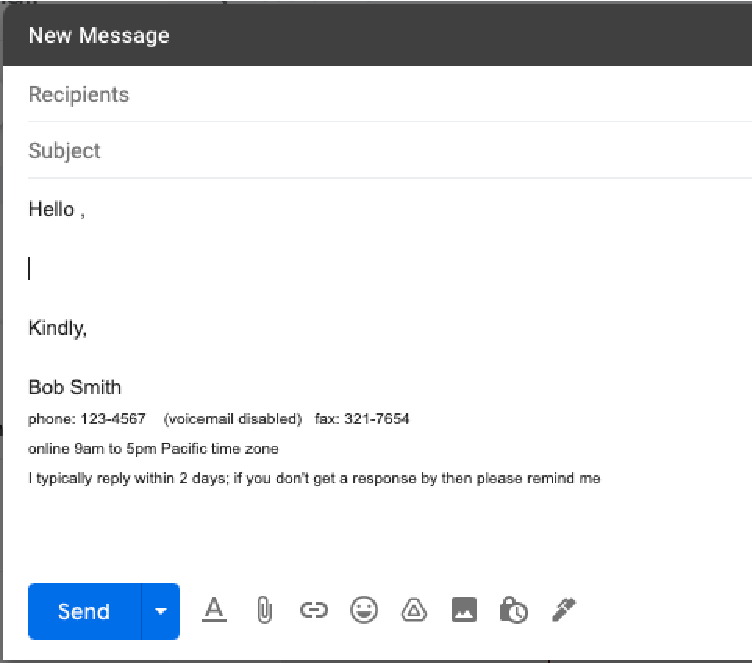
\includegraphics[width=1\textwidth]{images/email_template.pdf}
\caption{Template for new email messages. The greeting has a space after the comma -- that is where the recipient's name will go. Signature block uses a smaller font size after the name.}
\label{fig:email_template}
\end{figure}

\ \\
\begin{samepage}
\textit{Email Improvement}: Email signature blocks do not include unnecessary images, as that uses more storage for recipients.
\end{samepage}

\ \\
\begin{samepage}
\textit{Email Improvement}: Email threads focused on a specific instance of a recurring event include the date (YYYY-MM-DD) in the subject line. See Figure~\ref{fig:email_meeting_notes}.
\end{samepage}

\ \\
\begin{samepage}
\textit{Email Improvement}: Based on the purpose of the email, example key phrases for subject lines include: ``meeting notes" versus ``agenda" versus ``question about."
\end{samepage}

\ \\
\begin{samepage}
\textit{Email Improvement}: Revising an existing subject line can disrupt the ability of email software to thread conversations. However, sometimes the revision is worth breaking threading.
\end{samepage}

\ \\
\begin{samepage}
\textit{Email Improvement}: When replying to an ongoing thread, keep the original message as part of the thread to provide readers with historical context.
\end{samepage}

\ \\
\begin{samepage}
\textit{Email Improvement}: When replying to threads with sensitive messages, sanitize the included content by removing names or identifying details.
\end{samepage}

\ \\
\begin{samepage}
\textit{Email Improvement}: If an email has multiple requests or questions, at the top of the email (after the greeting) explicitly say how many of each type. Then, in the body of the message, number them. See Figure~\ref{fig:email_meeting_notes}.
\end{samepage}

% https://www.overleaf.com/learn/latex/Errors/%60!h%27_float_specifier_changed_to_%60!ht%27
\begin{figure}%[H] % formerly ht
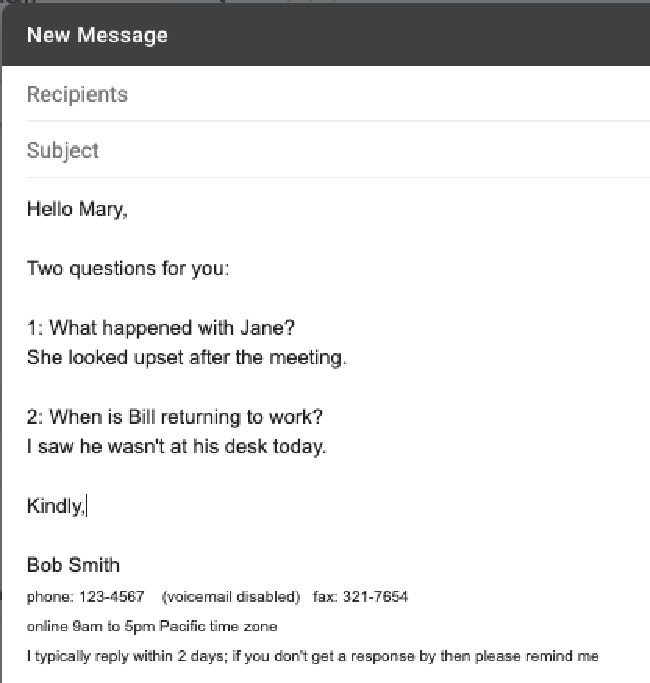
\includegraphics[width=1\textwidth]{images/email_two_questions.pdf}
\caption{Distinct items the recipient should address in a reply. A good subject for this email would indicate there are two questions you are seeking answers for.}
\label{fig:email_two_questions}
\end{figure}

\ \\
\begin{samepage}
\textit{Email Improvement}: If an item corresponds to a requested action, separately highlight the action and indicate who is supposed to take the action and what the deadline for response is.
\end{samepage}

% https://www.overleaf.com/learn/latex/Errors/%60!h%27_float_specifier_changed_to_%60!ht%27
\begin{figure}%[H] % formerly ht
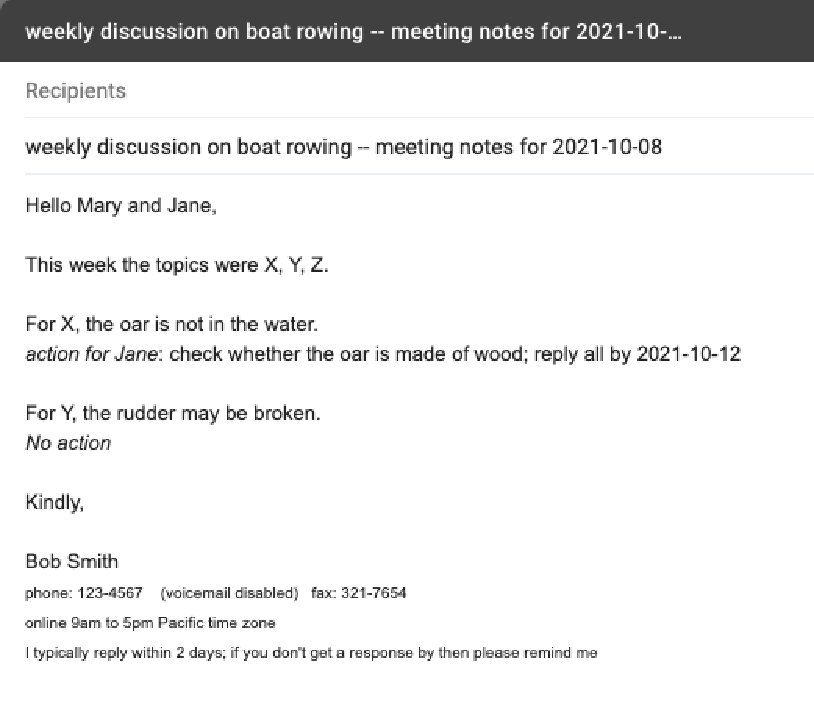
\includegraphics[width=1\textwidth]{images/email_meeting_notes.pdf}
\caption{Who has what action due when? The meeting notes are for a particular instance of a recurring event, so YYYY-MM-DD is included in the subject. Process Empathy involves thinking ahead about how future readers will differentiate this message from others.}
\label{fig:email_meeting_notes}
\end{figure}

\ \\
\begin{samepage}
\textit{Email Improvement}: Computer commands should use distinct separate fixed-width font. This distinguishes the text from the rest of the narrative.  See Figure~\ref{fig:email_computer_font}.
\end{samepage}


\begin{figure}%[H] % formerly ht
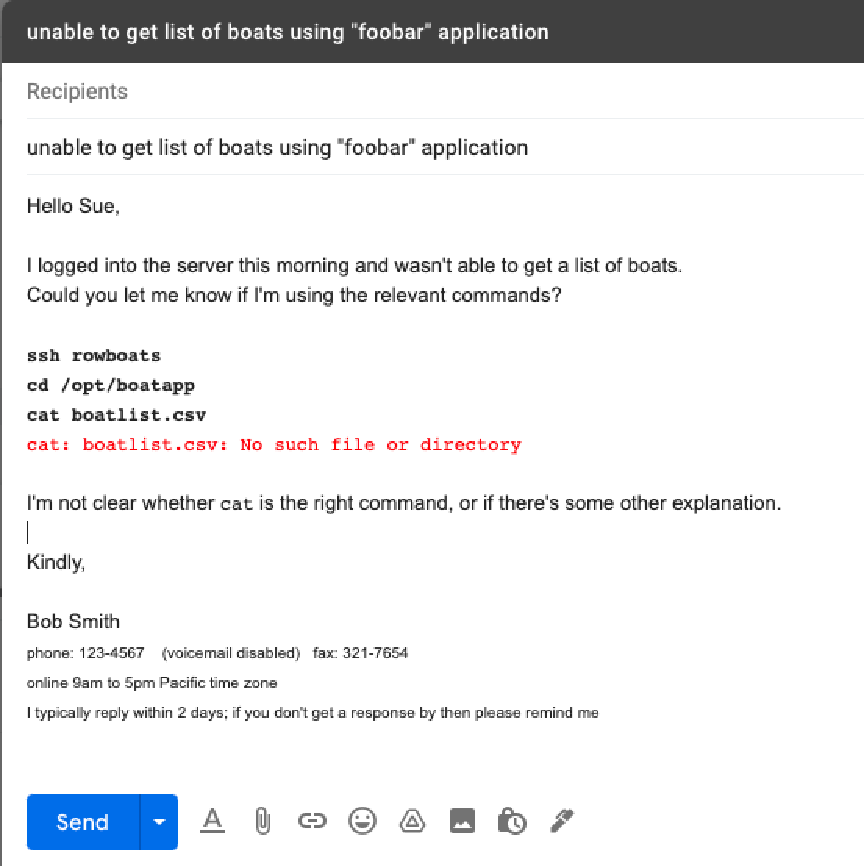
\includegraphics[width=1\textwidth]{images/email_computer_font.pdf}
\caption{The computer commands use fixed-width font. Input is distinguished from output using of bold and non-bold respectively. The error message is highlighted using red. Inline text like ``cat'' in the last line is also fixed width.}
\label{fig:email_computer_font}
\end{figure}

\ \\
\begin{samepage}
\textit{Email Improvement}: References to documents include a direct full path.
\end{samepage}

\ \\
\begin{samepage}
\textit{Email Improvement}: If referring to a previous separate thread, include the subject and the date+time that email was sent.
\end{samepage}

\ \\
\begin{samepage}
\textit{Email Improvement}: For bullet points, explicitly specify that items are joined by one of the following: OR, XOR, AND. For example,
\begin{itemize}
    \item Buy bread.\\
    \textit{and}
    \item Sell socks.
\end{itemize}
versus
\begin{itemize}
    \item Press the ``Return'' key.\\
    \textit{xor}
    \item Press the ``Space'' key.
\end{itemize}
\end{samepage}

\ \\
\begin{samepage}
\textit{Email Improvement}: If you have an unordered list, explicitly state that order is irrelevant.
\end{samepage}

\ \\
\begin{samepage}
\textit{Email Improvement}: If you have a sequence of steps, number them and indicate which steps are required versus optional. For example,
\begin{enumerate}
    \item (\textit{required}) Go to France.
    \item (\textit{optional}) Go to Greece.
    \item (\textit{required}) Go to Spain.
\end{enumerate}
\end{samepage}

\ \\
\begin{samepage}
\textit{Email Improvement}: Use visual sketches to illustrate concepts rather than always relying on text. Don't use pictures all the time, and don't have too many pictures in an email. 
\end{samepage}

\ \\
\begin{samepage}
\textit{Email Improvement}: Know how to both embed pictures inline and how to attach files and when to use which. 
Email replies should preferentially be at the top of the thread. 
If replying to multiple points in the previous email, embed replies inline, mark the distinction, and highlight the authorship. 
\end{samepage}

\begin{figure}[H] % formerly ht
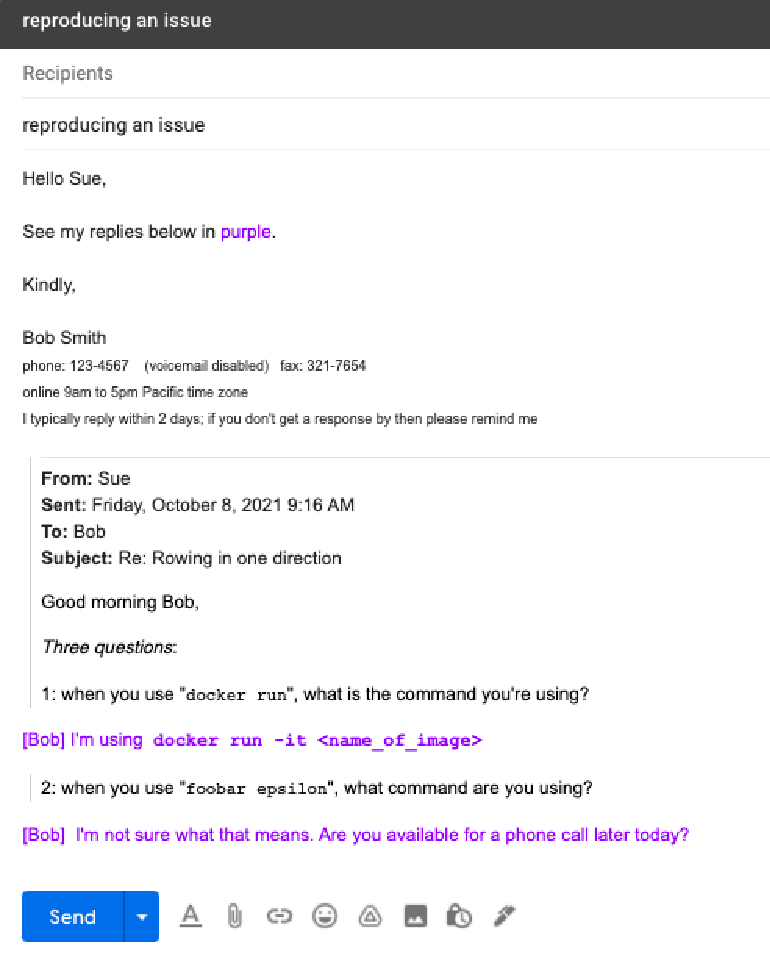
\includegraphics[width=1\textwidth]{images/email_reply.pdf}
\caption{Bob's reply to Sue's questions. The third question is not shown in this illustration.}
\label{fig:email_reply}
\end{figure}

\ \\
\begin{samepage}
\textit{Email Improvement}: If replying inline, explicitly state that at the top of the thread.
\end{samepage}

\ \\
\begin{samepage}
\textit{Email Improvement}: If the email is longer than a paragraph, provide a \href{https://en.wikipedia.org/wiki/BLUF_(communication)}{B.L.U.F}  (bottom line up front)
\index{Wikipedia!\href{https://en.wikipedia.org/wiki/BLUF_(communication)}{BLUF}}\iftoggle{WPinmargin}{\marginpar{$>$Wikipedia: BLUF}}{}
or 
\href{https://en.wikipedia.org/wiki/TL;DR}{tl;dr} (too long; didn't read)
\index{Wikipedia!\href{https://en.wikipedia.org/wiki/TL;DR}{tl;dr}}
or summary. In general emails should be short. Longer discussions should be held on the phone or in person, with a summary report after the discussion. Reliance on a BLUF or tl;dr risks resulting in the reader skipping the content. 
\end{samepage}

\ \\
\begin{samepage}
\textit{Email Improvement}: Every email should have a purpose. What are you asking the recipient to do? How do you want them to feel? How should they respond?
\end{samepage}

\ \\
\begin{samepage}
\textit{Email Improvement}: When replying, starting your email with an expression of gratitude for the work the recipient has done so far sets a positive tone by acknowledging their investment.
\end{samepage}

\ \\
\begin{samepage}
\textit{Email Improvement}: Read each email and report to determine the purpose. 
\end{samepage}

Reading each email is burdensome. If you don't have time to read everything, a common tactic is to skim the content. 
% https://graphthinking.blogspot.com/2021/03/read-each-email-to-determine-purpose.html
This tactic of skimming can lead to problematic behavior. First you scan the text of a message to see if there is immediate action or response needed. If no action or response is needed, go to the next email. 
That may not work for emails that have logistics associated with future events, or emails that alter your perception of the situation.

If you read an email to figure out the purpose of the email, that will help determine what action and response are relevant. Here I'm using ``action" to refer to activities outside the email channel. 


\subsection*{Why did this Email get sent?}
Below are potential intentions of the person writing the email. 

\ \\
\begin{samepage}
\textit{Email intent}: \textbf{Decision needed}. Typically includes context. \\
\textit{Action}: if the team maintains a decision log, update that.
Response is your selection of a choice.
\end{samepage}

\textit{Improvement for decision-centric emails}: Instead of asking for a decision, ask if the person is opposed. Or, even better, ask for the go-ahead. 
This framing biases the respondent towards action (specifically approval) rather than thinking. 
See 
\hyperref[sec:approval-forgiveness-opposition]{approval and forgiveness and opposition}
\marginpar{See page~\pageref{sec:approval-forgiveness-opposition}.}
for more details.

\ \\
\begin{samepage}
\textit{Email intent}: \textbf{Situational awareness}.\\
\textit{Action}: Expected default is no action, but interject if there's an issue.
\end{samepage}

\ \\
\begin{samepage}
\textit{Email intent}: \textbf{Action or Tasking}.\\
\textit{Action}: Do something within a specified deadline.
\end{samepage}

\ \\
\begin{samepage}
\textit{Email intent}: \textbf{Approval sought}.\\
\textit{Action}: Confirm or deny.
\end{samepage}

\ \\
\begin{samepage}
\textit{Email intent}: \textbf{Feedback sought}.\\
\textit{Action}: Assessment of proposal.
\end{samepage}

\ \\
\begin{samepage}
\textit{Email intent}: \textbf{Meeting logistics}. Can be an announcement (widely available), registration (limited attendance), or invitation (specific to you). Attendance is either optional or required. \\
\textit{Action}: Create or update a calendar event.
Response should restate the logistics (specifically the time and date and location and purpose) to confirm. 
\end{samepage}

\ \\
\begin{samepage}
\textit{Email intent}: \textbf{Brainstorming}.\\
May provoke a response for building on an idea.
``For your situational awareness, no action needed." Notification of activity by someone else. Or change in plans. 
If needed, a correction to the described direction might trigger a response or even a meeting.
\end{samepage}

\ \\
\begin{samepage}
\textit{Email intent}: \textbf{Reference}. E.g., describing a process, or a business workflow, or a citation.\\
\textit{Action}: Copy process documentation to wiki. Copy citation to bibliography.
Acknowledgement response thanking the sender for the update or clarification.
\end{samepage}

\ \\
\begin{samepage}
\textit{Email intent}: \textbf{Setting a formal policy or issuing an informal edict}.\\
\textit{Action}: move the policy or edict documentation to \href{https://en.wikipedia.org/wiki/Confluence_(software)}{Confluence}
\index{Wikipedia!\href{https://en.wikipedia.org/wiki/Confluence_(software)}{Confluence}}
or Wiki.\iftoggle{WPinmargin}{\marginpar{$>$Wikipedia: Confluence}}{}
Acknowledgement response needed only if the edit is aimed at just me or the group I am leading.
\end{samepage}

\ \\
\begin{samepage}
\textit{Email intent}: \textbf{Question}.\\
If this is a recurring question, move to a ``Frequently Asked Questions" page on a Confluence or Wiki.
Response is needed that provides an answer or seeks clarification.
\end{samepage}

\ \\

By categorizing the intent of emails and reports, you can respond more appropriately. Often the intent may be unclear, in which case a response can be framed as curiosity-based: ``I think you're seeking a decision, but here's the question that is crucial to ask before deciding."

\ \\

% TRANSITION to  \clearpage 
    

    \section{Meetings are Bureaucratic\label{sec:meetings}}
    %There are many books on how to do meetings well. 
    % "Making of a Manager" has chapter 6 (pages 139-159)
    % How is this section (in a book about bureaucracy) distinct?
    % how does understanding bureaucracy matter in the context of a meeting? what's the change in behavior for the effective bureaucrat?
    \Gls{bureaucracy} is distributed decision-making and distributed knowledge associated with management of shared resources. Bureaucrats rely on a variety of mechanisms to communicate, one of which is a meeting with other bureaucrats. 

    Every participant in an organization is invested the outcome of every decision made because there is consequence to how resources are divided and the direction of the organization. Every bureaucrat has an opinion, even when lacking experience or expertise. 

    \ \\

    The section describes \hyperref[sec:financial-models-of-communication]{financial models of communication}, essentials of \hyperref[sec:well-run-meeting]{a well-run meeting}, \hyperref[sec:characterizing-meetings]{types of meetings}, options when \hyperref[sec:bad-presentations]{listening to bad presentations}, and how to \hyperref[sec:effective-presentations]{make effective presentations}.

    %Stakeholders care about the outcome of a decision. 
        \subsection*{Financial models of communication\label{sec:financial-models-of-communication}}

This section analyzes communication from a financial perspective, focusing on two observations:
being late to a meeting is theft, 
and poorly written email and email to the wrong people has financial cost.
The point of raising these is to enable comparison with other investments the organization makes. Creating a cost model can help determine how much effort into improving what might otherwise seem like cultural issues.

\subsubsection*{Meeting time compared to theft}
% https://graphthinking.blogspot.com/2021/02/organizations-value-things-more-than.html

In large organizations there can be significant bureaucracy associated with even small purchases. A multi-step review process may be incurred for a \$200 acquisition. (Typically the cost of the review process in terms of person-hours spent isn't part of the calculus.)

Another measurement of value is that if an employee were to steal even \$200 worth of materials, the organization would likely punish that employee.

In the book High Output Management~\cite{1995_Grove}, Grove points out that those metrics apply to tangible goods, but not to people's time. Consider a meeting of 10 people and each person's cost is \$200 per hour. 
\marginpar{$>>$ Math}%
A wasted meeting is not unusual and would not incur bureaucratic review processes. The cost to the organization is fiscally the same -- \$2000. Similarly, consider an employee who is late and causes a loss of productivity. Merely depriving the organization of \$200 worth of time is not punished in the same way theft is.

In practice, organizations default to meetings (even recurring meetings) rather than not meet. And being late (by a few minutes) to a meeting is commonly accepted. 
We can debate the differences between theft of materials and theft of time. The financial argument is the two are indistinguishable. 


\subsubsection*{Email is not free}

Bureaucracy as distributed knowledge and distributed decision-making requires communication. Because synchronous communication like phone calls, video calls, and in-person meetings is challenging to coordinate, written communication is widely used for asynchronous collaboration. Whether that written content is emails or text-based chat, writing is expensive.

The cost of email includes
\begin{itemize}
    \item Time spent writing (authorship).
    \item Time spent reading (readership).
    \item Infrastructure maintenance.
\end{itemize}

Those three factors can be quantified as variables. 
\marginpar{$>>$ Math}%
\begin{multline}
\text{Cost per email} = 
(\text{hourly rate of writer})*(\text{time spent writing}) +\\
(\text{hourly rate of reader})*(\text{time spent reading})*(\text{number of readers})+\\
\frac{\text{annual salary of maintainer}}{\text{number of emails per year}} + \frac{\text{email server cost}}{\text{number of emails per year}}
\end{multline}
Plugging in some numbers, suppose an author charging \$50 per hour spends 5 minutes writing an email to 4 people. Each of those four people also charges \$50 per hour and spends 2 minutes on reading. 
\begin{equation}
50*(5/60) + 50*(2/60)*4 + \frac{100000}{1000000} + \frac{10000}{1000000} = \$10.84
\label{eq:four_readers}
\end{equation}
The cost to the organization is \$11 for one email! The breakdown of the three variables is shown in Figure~\ref{fig:my_label}. You've probably sent and received more than one email in your professional career as a bureaucrat. 


If the cost of one email doesn't lead you to be careful with communication, consider the cost to the organization of communication. If email consumes 2 hours a day per person (reading and writing), and if staffing is 50\% of the organization's budget, then 
    % (2/8)*0.5
12.5\% of the organization's budget is spent on email. The same math for applies to meetings, so with 2 hours of meeting and 2 hours of email that's 25\% of the organization's budget on coordination.

\begin{figure}
    \centering
    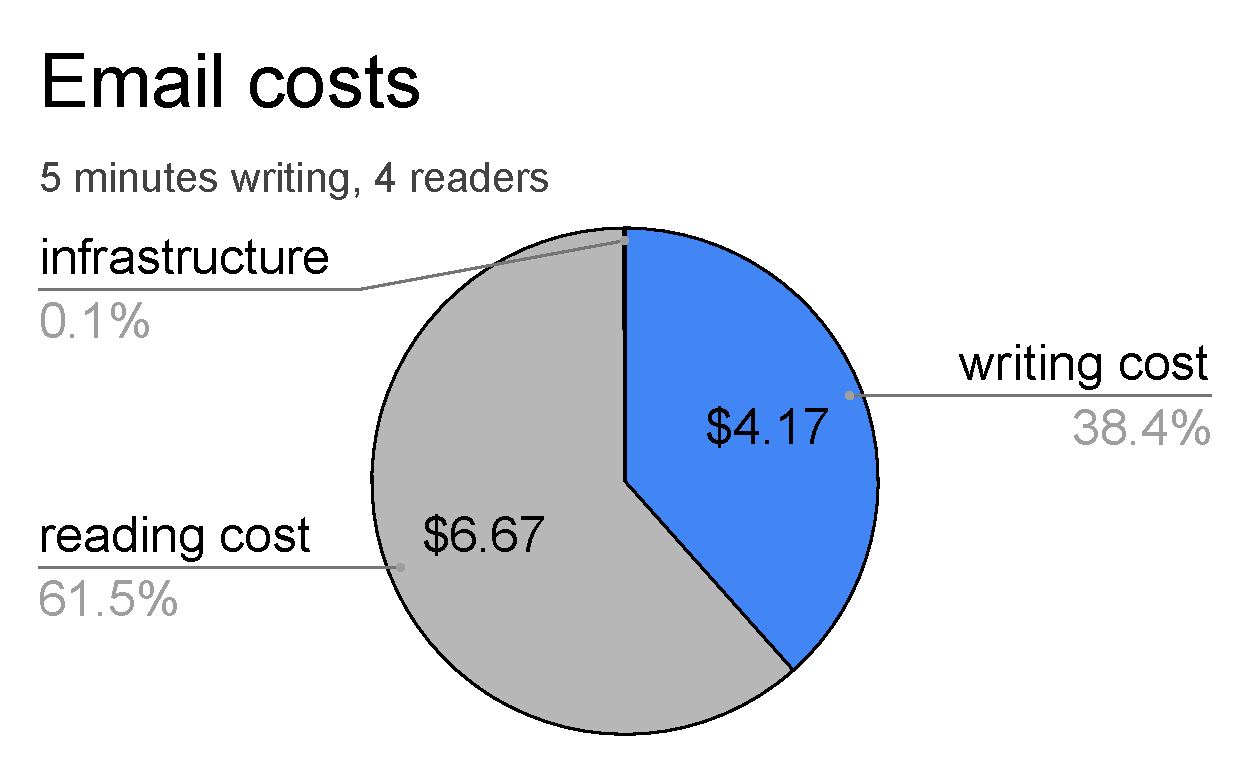
\includegraphics[width=0.7\textwidth]{images/email_costs_5minutes_4people.pdf}
    \caption{Breakdown of costs for Equation~\ref{eq:four_readers}. Assume an hourly rate of \$50 per person, and assume a reading time of 2 minutes.}
    \label{fig:my_label}
\end{figure}

% https://docs.google.com/spreadsheets/d/1ysV5PA3cEcneKv5BViUhAfgNq26cOlNRj6l5fXuHM3Q/edit?usp=sharing


 
        \section{Well-run meeting\label{sec:well-run-meeting}}

Explaining how to run an effective meeting (the scope of this section) is easy. Explaining why meetings are ineffective is a \href{https://en.wikipedia.org/wiki/Nash_equilibrium}{Nash equilibrium}. No one player benefits by reducing the number of meetings or effectiveness even though the group would benefit. So we all sit in ineffective meetings. 

The scope of this section is distinct from the processes covered by \href{https://en.wikipedia.org/wiki/Robert\%27s_Rules_of_Order}{Robert's Rules of Order}\footnote{I have not used Robert's Rules of Order for a meeting internal to a bureaucracy. Inside bureaucracies I'm aware of Robert's Rules of Order does not appear to be commonly used.}. 

\subsection*{Form relationships and understand constituents before the Meeting}

\href{https://en.wikipedia.org/wiki/Nemawashi}{Nemawashi}

\subsection*{Don't invite everyone}
Identify essential attendees. If someone does not need to be present, tell them in advance that you will share the meeting notes afterwards. 

\subsection*{Create and use an Agenda}
\textit{Bad}: no meeting agenda\\
\textit{Good}: Have an agenda. \\
\textit{Better}: \underline{Share the agenda with other participants}. Having an agenda keeps attendees focused.  Enables tracking of progress during the meeting so participants are more likely to get to all topics.\\
\textit{Best}: For formal meetings, \underline{share the agenda in writing before meeting}. Sharing the agenda in advance allows attendees to prepare.

Forces conspiring against agendas: takes time to create an agenda. Attendees might not take the time to read beforehand. Attendees may not stick to the agenda during the meeting.

\subsection*{Ensure facilities are adequate}
For formal in-person meetings verify meeting venue has enough space, seating, working IT equipment. For formal virtual meetings ensure participants are familiar with virtual meeting controls. 
%  why logistics and infrastructure matter in a bureaucracy
As a bureaucrat you may not see taking care of details like this as your responsibility. Ensuring well-run logistics and effective use of infrastructure may not be your area of expertise, you lack training in this domain, it's not in your job description, and you won't get promoted for taking care of it. 

Attention to detail outside the scope of your official duties benefits your reputation. Proactive concern for the smooth operation of the bureaucracy enables efficiency in time and resources.

% TODO: forces conspiring against logistics and infrastructure

Fire alarm or other emergencies. 

\subsection*{Body language matters}

If you are not speaking, are you reclined or leaning forward on the edge of your seat? Are you looking at the speaker?

If your eyes are closed, other people don't know if you're picturing something or falling asleep. 

If you approve of something but don't want to verbally interject, a thumbs up is useful signaling. 

\subsection*{Take and share Meeting Notes}

Meeting notes are more detailed than the agenda but less detailed than a transcript of who said what. Meeting notes synthesize the discussion. Meeting notes specify follow-on who is taking which actions with what deadlines. 

See also the discussion on \hyperref[sec:written-comm-does-not-happen]{why meeting notes do not get taken}.
%, see section~\ref{sec:written-comm-does-not-happen}. 

\subsection*{Facilitator ensures Presenters are Capable}

Does the presenter know how to project materials? How to present slides?

\subsection*{Facilitator's ground rules}

To run a smooth and productive meeting, I explicitly state two ground rules to the attendees:
\begin{itemize}
    \item If you want to talk, raise your hand and I will call on you. If there are multiple people wanting to talk, I'll track the order of speakers.
    \item If you talk too long, I'll cut you off. 
\end{itemize}
This approach is critical when there are many people present, when people with diverse backgrounds are present, or when there is a mixture of dominant and submissive personalities present. 
If a visual signal like hand raising is not used, reliance on verbal interruption defaults to dominant personalities. Waiting for a person to finish speaking doesn't work for everyone because some participants will use more than their fair share of time. speaking for a long time needs to be addressed regardless of whether an intentional effort to exclude others or a consequence of verbosity.

As a facilitator, my focus is on structure (distinct phases of the discussion) and ensuring participation. I remove myself from taking part in the discussion.

\subsection*{Facilitate Asking Dumb Questions without Feeling Intimidated}

Asking a question of an expert from a position of ignorance can feel intimidating. You may worry you're wasting the expert's time. In a recurring meeting a facilitator can address this by having participants write questions on paper and submitting anonymously. The questions or discussion topics can then be raised at following meetings. 

To facilitate the anonymity every participant must be given paper and pen, and every participant must write something on the paper. The facilitator then has to collect the paper from each participant. For contributors who don't have a question, they can write down feedback about the meeting. 

This technique allows the expert to get the information needed for a response, or to figure out who the best person to respond is. 

\subsection*{Collect feedback from Attendees on How to Improve}

Follow up with meeting attendees to get feedback on how to improve. % subsection
        \subsection*{Characterizing Meetings}
% relevance of this section:
Characterizing meetings is critical to distinguishing which norms are applicable, and what people expect from the different formats. 



Types of meetings: internal meetings, customer meetings, conferences, scheduled one-on-ones, impromptu walk-around.   


%What is the purpose of a meeting?
% https://graphthinking.blogspot.com/2019/12/what-is-purpose-of-this-meeting.html
There are many potential purposes of a meeting, including
\begin{itemize}
    \item To gather input from attendees.
    \item To make a pronouncement to attendees.
    \item To educate attendees.
    \item To educate one person.
    \item To signal interaction.
    \item To brainstorm ideas.
    \item To make progress towards an goal.
\end{itemize}
When the purpose is not explicitly stated, confusion arises. 
When multiple purposes occur in one meeting and the transition is not explicitly stated, confusion arises.
The reason for this confusion is that the assumptions and expectations and norms of each purpose are different. When the attendees don't know the purpose or the purpose shifts, the expected behaviors and roles are unclear. 

An attendee can ask what the purpose of the meeting is during the meeting but that is generally considered rude. An attendee can try to deduce the purpose of a meeting, but this takes time and attention and can result in the wrong conclusion. An attendee can try to set the purpose of the meeting during the meeting, but this can conflict with the intent of other attendees. 

A meeting's purpose can shift during a meeting. If done intentionally, the changes should be stated explicitly. Otherwise an attendee may continue to work under the previous set of expectations rather than the current norms. 



% https://graphthinking.blogspot.com/2014/12/how-to-understand-meetings-at-work.html
Level of formality, start time (early or on time or late), 
end time (early or on time or late), utility, 
duration, number of attendees, number of speakers, number of participants.



Meetings involve people, either known or strangers.
Meetings involve information, either relevant or irrelevant. Relevant information is either new or related to previous work.
Meetings either have a leader or no leader (brainstorming). If there's a leader, the leader may be disseminating info to participants, or gathering information from attendees.


\subsubsection*{Phases of a meeting}

\begin{enumerate}
    \item Establish understanding of what the topic is. Without a shared focus and a common goal a meeting is unlikely to be productive. 
    \item Set aside topics that are not the focus. Either discuss outside the current meeting or defer to a later meeting. Managing scope is critical to accomplishing the goal. 
    \item Establish a shared language specific to the topic and to the participants.
    \item Establish each participant's viewpoint on the topic.
    \item Brainstorm options.
    \item Build consensus or nominate a decider.
\end{enumerate} 
        \subsection*{Walk-around impromptu meetings\label{sec:walk-arounds}}

Meetings aren't constrained to occur in conference rooms around a table with everyone seated. Walking around the shared office space and having conversations with coworkers can be an intentional form of informal meeting. 

Ambushing coworkers when they aren't expecting interruption takes tact. As the (potential) interrupter, you need to be sensitive that other people may not want to be interrupted, while others seek diversion from their current task. If you're the person being interrupted by the coworker walking around, you have the right to deferral. 


Walking around and finding people to talk with can be for 
\hyperref[sec:socializing]{social engagement} 
\marginpar{See page~\pageref{sec:socializing}}
or to discuss tasks you are working on. 
In either case, you are interrupting existing activities. Presence creates priority,
\index{mantra!presence creates priority}
whether intentional or accidental.


%The \href{https://en.wikipedia.org/wiki/Allen_curve}{Allen curve}; 



% https://graphthinking.blogspot.com/2016/04/role-models-for-great-leaders.html
This concept isn't new. 
In the American Revolution, \href{https://en.wikipedia.org/wiki/Friedrich_Wilhelm_von_Steuben}{Baron von Steuben}
\index{Wikipedia!\href{https://en.wikipedia.org/wiki/Friedrich_Wilhelm_von_Steuben}{Baron von Steuben}}\iftoggle{WPinmargin}{\marginpar{[Wikipedia] Baron\\ von Steuben}}{}
and 
\href{https://en.wikipedia.org/wiki/George_Washington}{George Washington}
\index{Wikipedia!\href{https://en.wikipedia.org/wiki/George_Washington}{George Washington}}
%%%CANTDO\marginpar{[Wikipedia] George \\Washington}
used walk-around meetings to understand the needs of the members of their army.\footnote{\href{https://www.battlefields.org/learn/articles/winter-valley-forge}{https://www.battlefields.org/learn/articles/winter-valley-forge}: ``Like Steuben, Lafayette engaged directly with his soldiers and became well known for enduring the same hardships as his men.''}
 
        \subsection*{One-on-one check-in meetings\label{sec:meetings-one-on-one}}

% CONTENT CHOICE: I'm avoiding tips on "how to manage" and "how to coach"?
% I have a lot of potential content on 
% https://graphthinking.blogspot.com/2021/09/notes-from-half-day-course-on-coaching.html

Formal one-on-one meetings of a supervisor and a team member. Opportunity for the supervisor to coach the team member and for the supervisor to learn what the problems are on the team. From the team member's perspective, a one-on-one is an opportunity to ensure alignment with the team's direction and to provide insight on how to improve the team. Education in both directions. 

% https://graphthinking.blogspot.com/2021/09/notes-from-half-day-course-on-coaching.html
One-on-one discussion take lot of time, so the mindset ``no news is good news" or ``everything is going well, no need to engage" is tempting. As a consequence only negative feedback causes interaction. 

% https://graphthinking.blogspot.com/2021/05/the-agenda-for-one-on-one-meeting.html

One-on-one meeting questions for helping the supervisor understand the team member's status. 
The one-on-one check-in should be tailored to the phase of the employee's progression. Frequency of check-ins depends on the newness of the team member, the complexity of the work, or how quickly the conditions are changing.
\begin{enumerate}
    \item \textit{Name of phase}: \underline{Welcome to the team!}\\
    \textit{Scenario: New team member, either new to the team or new to the organization. }\\
    Here the focus of the one-on-one is to ensure a smooth on-boarding process. Get them up-to-speed on the technical challenges, professional norms, and integrated with other team members. Resolve administrative blockers: Does the employee have the necessary computer log-in accounts? Do they have an email account? Are they on the mailing list? \\
    Questions:
    \begin{itemize}
        \item What are the goals for the team?
        \item What items on the onboarding checklist are not yet completed?
        \item Who have you met on the team? What is your understand of their role on the team?
    \end{itemize}
\textit{The duration of this phase could last between a day and two weeks.}
    \item \textit{Name of phase}: \underline{Initial contributions}\\
    \textit{Scenario: Team member handles small tasks. }\\
    The one-one-one is for discussions on training and planning and task reviews. Characterized by the team member being dependent on others for their success. In this phase the employee collaborates on tasks.\\
    Questions:
    \begin{itemize}
        \item What are the goals for the team?
        \item What are your task goals?
        \item What are you expecting to deliver to the team? When? 
        \item What dependencies does that deliverable have (external to the team or internal to the team)?
    \end{itemize}
\textit{The duration of this phase could last a few months to years.}
    \item \textit{Name of phase}: \underline{Experienced contributor}\\
    \textit{Scenario: Team member handles large tasks (which get broken into subtasks). }\\
    The one-on-one is to help the team member define their success. Activities include planning, resource allocation, assessment. Characterized by the need to coordinate with others on the team or other teams. Team member understands task scope and intent and relevant processes. Team member decomposes task into subtasks.\\
    Questions:
    \begin{itemize}
        \item How do the artifacts you're working on support your plan for the team's progress?
        \item What dependencies does that deliverable have (external to the team or internal to the team)?
        \item What insights do you have about the team or organization?
        \item What insights do you have about the relevance of the task relative to the intent of the organization?
        \item What should management be doing to enable the team's success?
    \end{itemize}
\textit{The duration of this phase could be the rest of a career.}
    \item \textit{Name of phase}: \underline{Facilitator}\\
    \textit{Scenario: Facilitating the productivity of others.}\\
    Rather than being task-oriented, this team member supports coworkers. \\
    Questions:
    \begin{itemize}
        \item What observations from mentoring team members do you have?
        \item What collaborations should we be fostering?
    \end{itemize}
    \item \textit{Name of phase}: \underline{Peer}\\
    \textit{Scenario: Peer check-in.}\\ 
    This one-on-one is a form of mentorship. The value of the exchange is to get a different perspective and to hold each other accountable.
\end{enumerate}

To evaluate when a team member and their supervisor should move to the next phase in the evolution, have an explicit conversation about the threshold for progression.


In addition to phase-specific questions, there are questions that fit all phases. A supervisor should ask the team member
\begin{itemize}
    \item What have you been successful with since we last met?
    \item What is blocking our team's progress?
    \item What are your plans?
    \item How are you collaborating with the rest of the team?
    \item If there was just one thing you could change about our organization, what would it be and why?
    \item How do you plan to train your coworkers on topics you understand and they don't?
    \item What have you learned in the past month?
    \item What are the biggest risks for the team?
    \item What's limiting your productivity?
\end{itemize}
Responding to these questions takes time (an hour) and willingness to be open. 

If the supervisor doesn't ask these questions, the team member has the ability to include these in the agenda and to bring them up. 


\ \\

A one-on-one meeting requires preparation. Before the meeting the team member should document
\begin{itemize}
    \item What was discussed previously.
    \item What progress has been made since the previous meeting.
    \item What is blocking progress.
\end{itemize}


%\ \\

% lots of comments, not much useful info
% https://news.ycombinator.com/item?id=30152268

\ \\

\subsubsection*{One-on-one meeting questions to spur discussion}

Not sure what to discuss? An extensive list of questions on topics like career development, conversation starters, and job satisfaction are available on \href{https://github.com/VGraupera/1on1-questions}{https://github.com/VGraupera/1on1-questions}\footnote{\href{https://news.ycombinator.com/item?id=22341138}{comments}}. 
        \subsection*{Listening to Bad Presentations\label{sec:bad-presentations}}

Occasionally you attend a meeting with a bad presentation. The slides may appear slick but the content is poorly thought out. Or the presenter does not understand the topic well. Or the presenter has good content but does not convey it well. Or the presenter is wrong about the topic. Regardless of the cause, you should assume the presenter is making their best effort. 

You could remain silent, complain, criticize, ask leading questions, or offer constructive feedback. Your silence may result in other attendees and the presenter leaving with incomplete or wrong information. If you speak up you'll prolong the meeting or limit the presenter's time to convey their material. 

Your assessment of the presentation may be wrong. You may lack relevant information. A reliable technique for interjection is to assume a state of confusion instead of confidently asserting that the presenter is wrong. 
If you believe the presenter is wrong, asking about the source of their information is a good entry point.

You should ask for clarification when the information is correct but presented poorly (or above the level you understand). 

\ \\

% TRANSITION

By paying attention to a bad presentation, you can  identify issues that you do not want to repeat. The next section summarizes a few insights so you don't need to learn from bad presentations.
        \subsection*{Make Effective Presentations\label{sec:effective-presentations}}

% https://graphthinking.blogspot.com/2011/10/presentation-notes.html

Speaking is vital at decision points in your career progress -- at interviews, competitions, gaining new collaborators at conferences. 
Because you want to avoid mistakes in those situations, you will need to prepare and practice.
Aim to impress your peers, supervisors, and the bureaucrats you oversee. 

Breaking down the variables of your presentation can help identify questions to consider. 
\begin{itemize}
    \item \textbf{Purpose}: What's your goal? What does your audience want? Are those aligned? 
    \item \textbf{Scope}: What is the minimum information you need to convey your point, while balancing that against the need to provide enough evidence of your claims?
    \item \textbf{Audience}: What's their background? What are they seeking? What are they expecting?
    \item \textbf{Speaker}: What should your appearance be? Do you need to alter your normal enunciation, volume, or rate?
    %, verbal accent, enunciation, smell.
    \item \textbf{Slides}: What is the layout of your content? What's the content? 
    \item \textbf{Props}: Are there artifacts that demonstrate the point of your presentation?
    \item \textbf{Venue}: How big is the room? What technology is available? How is the lighting? Will you be competing with a noise source? Other visual distractions?
    \item \textbf{Time}: How much time do you have to prepare? Do you have access to the venue before the event? How much time do you have for presentation? For questions?
\end{itemize}

% from https://graphthinking.blogspot.com/2023/01/more-questions-to-ask-when-you.html
\label{sec:extending-Heilmeier}
Expanding on the question of purpose for your talk, a standard framing is 
\href{https://en.wikipedia.org/wiki/George_H._Heilmeier\%23Heilmeier's_Catechism}{Heilmeier's Catechism}.
\index{Wikipedia!Heilmeier's Catechism@\href{https://en.wikipedia.org/wiki/George_H._Heilmeier\%23Heilmeier's_Catechism}{Heilmeier's Catechism}}
Heilmeier's list of questions is concise enough to be memorable, but skips some relevant aspects. The list I recommend reflecting on builds on the original set:
\begin{itemize}
    \item (Heilmeier asks) What are you trying to do? Articulate your objectives using  no jargon.
    \begin{itemize}
        \item Should the solution be technical, social, or a process?
        \item Which aspects are quantifiable and which are qualitative?
    \end{itemize}
    \item (Heilmeier asks) How is it done today, and what are the limits of current practice?
    \begin{itemize}
        \item How did we get to the current situation? 
    \end{itemize}
    \item (Heilmeier asks) What's new in your approach and why do you think it will be successful?
    \begin{itemize}
        \item What has been tried before? Why did those efforts not succeed?
    \end{itemize}
    \item (Heilmeier asks) Who cares? If you're successful, what difference will it make?
    \begin{itemize}
        \item Who are the stakeholders? What involvement do you expect from each stakeholder?
    \end{itemize}
    \item (Heilmeier asks) What are the risks and the payoffs?
    \item What are the constraints?
    \begin{itemize}
        \item (Heilmeier asks) How much will [each milestone] cost?
        \item (Heilmeier asks) How long will [each milestone] take?
        \item What skills are needed for each milestone?
        \item How do you know that set of constraints is correct? Complete?
    \end{itemize}
    \item (Heilmeier asks) What are the midterm and final ``exams" to check for success?
    \begin{itemize}
        \item Who is evaluating the milestone artifacts?
        \item What will be measured to determine the success of each milestone?
        \item You should pre-register what counts as failure to enable accountability.
    \end{itemize}
\end{itemize}








In addition to the questions above, another way to think ahead is the sequential tasks associated with the presentation. 
The following can serve as a checklist.

\subsubsection*{Planning your presentation}

Evaluate your audience's experience and education before creating the presentation. The question you are addressing in your presentation may be independent of the audience, but the level of delivery depends on the audience's background.

When speaking to an audience outside your field, aim to use jargon your audience is familiar with. Another tactic is to look for areas of commonality and then build on that.

When introducing your topic, there are a few ways to open the talk:
\begin{itemize}
    \item \textbf{Compliment} the audience.
    \item \textbf{Humor}: tell a relevant joke.
    \item \textbf{Vulnerability}: Tell how this work makes you feel.
    \item \textbf{Numbers}: Explain context and relevance in terms of money, number of people involved, and size of the system.
\end{itemize}


%\begin{itemize}
%    \item . For example, a physicist uses ``quantization of energy" whereas an audience of mathematicians may be more comfortable with ``discrete energy levels."
%    \item Look for commonality. For example, both physicists and mathematicians use assumptions and build models.
%\end{itemize}

Prepare the content:
\begin{itemize}
    \item Tell a coherent story with a unified theme. Each slide should be logically connected to the following slide. Don't just put a bunch of slides with data or pictures together. You risk disorienting your audience.
    \item Run spell check before presenting.
    \item Translate your slides from your native language to the language of your audience.
\end{itemize}


For the visual content in presentations:
\begin{itemize}
    \item Switching between dark and light slides in a dark room stresses the eyes. The audience needs time to adjust to varying light levels.
    \item Images should use both color contrast and distinct symbols; this is called redundant coding. 
    \item Pick colors that are accessible for colorblind audiences. For example green and magenta are better than green and red. 
    % https://jfly.uni-koeln.de/color/
    % prevoiusly http://jfly.iam.u-tokyo.ac.jp/color/
    \item Making slides appear ``professional" means adding non-informational content. This added content should be consistent, not distracting.
\end{itemize}

%Software:
Common choices include \LaTeX (specifically \href{https://en.wikipedia.org/wiki/Beamer_(LaTeX)}{Beamer}), 
\index{Wikipedia!Beamer@\href{https://en.wikipedia.org/wiki/Beamer_(LaTeX)}{Beamer software}}\iftoggle{WPinmargin}{\marginpar{$>$Wikipedia: Beamer}}{}
Microsoft \href{https://en.wikipedia.org/wiki/Microsoft_PowerPoint}{PowerPoint}, 
\index{Wikipedia!PowerPoint@\href{https://en.wikipedia.org/wiki/Microsoft_PowerPoint}{PowerPoint software}}
and Apple's \href{https://en.wikipedia.org/wiki/Keynote_(presentation_software)}{Keynote}. 
\index{Wikipedia!Keynote software@\href{https://en.wikipedia.org/wiki/Keynote_(presentation_software)}{Keynote software}}
%Less well-known are Prezi (and its open source equivalent, InkScape+Sozi add-on).
You are sending a few messages to your audience if you use Microsoft Word, a document PDF, Notepad, or any other non-presentation software to make a presentation.
The two messages are first, the audience isn't worth the time you needed to develop a proper presentation, and second, you are not technically savvy.

\ \\

%Presenting multiple topics within one presentation:
%Disparate topics require a segue to show why you are transitioning.
%Inter-relate the multiple topics 

Live demos can invigorate a boring presentation. Besides the interactivity aspect, the audience is excited by the risk of technical failure. 
If you plan to give a live demo, have screenshots of the process in the presentation. That way, if the demo fails you can show what was supposed to happen in the slides. If the demo works, skip the slides.


Practice the presentation (out loud in real-time) at least once.
Use the setup as close to reality as possible for practice sessions. Project onto the screen using the projector. This experiment will show if the color contrast is sufficient.

\ \\
%Prior to giving a talk at a remote (or unfamiliar) environment

Questions to ask your host:
\begin{itemize}
    \item Will I have a projector and screen for the presentation?
    \item For the technology I'm using (PowerPoint, PDF, Keynote), which version is provided? 
    Or does the speaker bring their computer? 
    Or is there internet access?
    \item How to best get the presentation content to the host? Bring a USB drive or laptop, or email the presentation file to the host?
\end{itemize}


\subsubsection*{Day of talk}

Appearance (suit and tie or jeans and t-shirt?):
\begin{itemize}
    \item Underdressed = I don't respect the audience.
    \item Overdressed = I'm better than you.
    \item Similar level of dress = I'm a peer.
\end{itemize}

\ \\

Some of these suggestions should seem glaringly obvious. They are here because I have seen them in ``official" presentations given by a ``professional." For example, do not curse. No profanity while speaking, in the slide presentation, or even the name of the file.

\subsubsection*{Before the talk begins}
\begin{itemize}
    \item Ensure your facility has power, a screen, a projector, a pointer, and any other necessary equipment. (Don't rely on your host to think of these things for you.)
    \item Ensure all equipment works and functions together.
    \item Before the presentation begins, use a slide to make announcements and reminders:
\begin{itemize}
    \item List the agenda if there are multiple speakers.
    \item Time talk begins, how long it will last.
    \item Reminder: Turn OFF Cell Phones. Airplane mode is insufficient since previously set alarms can ring.
\end{itemize}
    \item Announce whether to ask questions during the talk (i.e., the audience should interrupt) or to hold questions until done.
\end{itemize}

\subsubsection*{During the talk}
\begin{itemize}
    \item Opening: Thank hosts, inviters, and organizers. Establish a connection between you (the speaker) and the audience.
    \item Do not pace.
    \item Do not stand frozen.
    \item If you are the only person laughing at your joke, it isn't funny.
\end{itemize}

 \subsubsection*{End of Your Presentation}

\begin{itemize}
    \item Let the person asking the question finish. Even if you think you know what they are going to ask, wait.
    \item Restate the question to make sure the audience heard it and that you understood it.
    \item Aim for shorter responses. Save your longer answer for a follow-up discussion after the audience has been released.
\end{itemize}


%\subsubsection*{After the Presentation}


  % multi-person interactions = process
  \chapter{Bureaucratic Processes\label{sec:process}}
  {\footnotesize Back to the \hyperref[sec:toc]{Main Table of Contents}}
  \minitoc
    % Claim: you already have habits; these are similar to processes use by bureaucrats in organizations

Because bureaucratic policies and processes seem convoluted, let's start from a more relatable point: your own personal habits.
You might eat at the same time every day, or you might go to bed at the same time. Those are both examples of personal policies. Sticking to a routine decreases the need to think about options. In the same way, bureaucrats in organizations seek routines to decrease uncertainty. 

You have experience with creating and using personal policies (your habits).  Bureaucratic processes for organizations are similar.
Both are routines which ease the burden of decision making. A habit can be intentional (e.g., my policy is to brush my teeth before going to bed), just as a process can be designed. Habits can be unconscious (e.g., arriving at work without recalling driving there), just as processes can arise without an intentional design. 

Consider your own intentional habits -- they are likely motivated by a personal policy. Similarly, bureaucrats acting on behalf of an organization apply processes that support policies of the organization.

\ \\

The sections of this chapter address the what (page~\pageref{sec:definition-of-process}), why (page~\pageref{sec:why-processes-exist}), and how (page~\pageref{sec:process-chaos}) of processes. 
The last sections of this chapter (design on page~\pageref{sec:design-of-processes} and change on page~\pageref{sec:change-a-process}) assume a level of control and autonomy that you may not think of you have. Regardless of where your role is in the hierarchy, your purpose is to provide value to the organization. That value can be negotiation with fellow bureaucrats on improvements to the design of task workflows. 

The foundation of your \gls{process empathy} is based on the sections in this chapter, whereas previous chapters have been focused on your skills as a bureaucrat.  \clearpage
    \section{Definition of Process and Policy\label{sec:definition-of-process}}


Bureaucratic organizations manage shared resources (tangible or expertise). 
A subjective decision about a resource that is administered by bureaucrats is formalized as a \gls{policy}.
The policy of an organization constrains what action is required, allowed, or not allowed with respect to the shared resource being managed by the organization.

% definition
To determine which policies apply in a given circumstance, a sequence of tasks (referred to as a \gls{process}) are defined. 
% Also known as a procedure. 
In a confusingly circular dependence, tasks may invoke policy enforcement by bureaucrats. 

Processes inform the decision-making of bureaucrats and result in access to or denial of shared resources. 
A process has inputs and outputs. 
A process can be decomposed into other processes. 
Processes operate on both information and tangible objects. 
Processes require \href{https://en.wikipedia.org/wiki/Work_(physics)}{work}
\index{Wikipedia!work, physics@\href{https://en.wikipedia.org/wiki/Work_(physics)}{work}}
and time. 
Processes are carried out by people or machines.

Processes are important for organizations because they create a defensible story for the bureaucrats involved. Processes are not correlated with fair distribution of the shared resource managed by the bureaucracy. Management of shared resources require policies, and enacting policies require processes. The processes are one step removed from the management of the shared resources. 


The alternative to process is an \hyperref[sec:exceptions-to-process]{exception}\iftoggle{haspagenumbers}{ -- see page~\pageref{sec:exceptions-to-process} for more details.}{.}
Creating and maintaining processes is burdensome, as is dealing with exceptions. This is the \hyperref[table:dilemma-personal-policy-consistency-across-cases]{Dilemma of Consistent Policies}\iftoggle{haspagenumbers}{; see page~\pageref{table:dilemma-personal-policy-consistency-across-cases}.}{.}

\ \\

% https://graphthinking.blogspot.com/2019/04/dealing-with-rules.html
In your role as bureaucrat or subject you have options for responding to policies and processes. You can:
\begin{itemize}
    \item Accept them. The default for most bureaucrats in an  organization.
    \item Intentionally break them maliciously (to cause harm). Typically limited to a small number of participants. These defectors have various motives -- frustration, moral opposition, personal revenge, etc.
    \item Intentionally break them for disruptive innovation. 
    From the view of other bureaucrats, your intent of innovation may be indistinguishable from malice. 
    \item Be ignorant of them. This may initially be easier for you (there's less to think about) but causes friction for everyone else and results in you being less effective. 
    \item Work in an environment where the rules have not yet been set. Then you are either limited in scale and complexity, or you will need to form new policies and processes as the organization grows.
\end{itemize}

\ \\

% process and roles
Processes are typically divided into separate tasks. With sufficient scale and complexity, each task becomes associated with distinct roles. The distinction of roles originates in skill specialization, separation of responsibilities, and enabling narrow authority. 

When there is insufficient staffing then individual bureaucrats have multiple roles. This can lead to a conflict of interest among the roles held by one person and is experienced by the bureaucrat as a \href{https://en.wikipedia.org/wiki/Cognitive_dissonance}{cognitive dissonance}. 
\index{Wikipedia!cognitive dissonance@\href{https://en.wikipedia.org/wiki/Cognitive_dissonance}{cognitive dissonance}}
For example, when one person has both the responsibility to enact a plan and review the completed implementation, the oversight is ineffective.\footnote{For a formal mechanism of documenting roles, see the Wikipedia entry for the 
\href{https://en.wikipedia.org/wiki/Responsibility_assignment_matrix}{Responsibility Assignment Matrix}.
\index{Wikipedia!responsibility assignment matrix@\string\href{https://en.wikipedia.org/wiki/Responsibility_assignment_matrix}{responsibility assignment matrix}}
}

\ \\

% how does understanding process help me?
The above observations are theoretical and generic, but there's already practical relevance to your actions as a bureaucrat.
\begin{itemize}
    \item Understanding concepts like process and policy helps you know when to work within versus work around, when to accept versus change, when to ignore, how to leverage, and how to design.
    \item In your role as a bureaucrat you administer a process. When you do that, check that the person you are inflicting the process on can explain the steps back to you. If they cannot, their confusion will likely create more work for the bureaucrats involved. 
\marginpar{$>>$ Actionable Advice}%
\index{actionable advice}
    \item As the subject of a process, check that your understanding of the process is consistent with the bureaucrat's intent. Summarize the next steps and applicable deadlines so they can confirm. 
\end{itemize}

\ \\

% dangers of process
The simplifications necessary for making policies and the neglect of specific circumstances results in \gls{process friction}. Process friction manifest in waste of resources (tangible or expertise), temporal inefficiency, emotional frustration, and social distrust of institutions.


%Two distinguishing features in the context of bureaucracy are authorization and justification.  

\subsection*{Types of Process}
% https://graphthinking.blogspot.com/2016/07/three-process-types-in-large-complex.html
The generic definition of \gls{process} used above obscures distinct subcategories. In practice, there are three types of processes: heroic, bureaucratic, and social.

\index{process type!heroic}
A \underline{heroic process} is exemplified by a single person or a small number of people doing the work associated with a specific task. The person may be acting in multiple roles and typically relies on expertise from multiple domains. This approach is not sustainable as there's significant dependence on the hero(s). The heroic process is a common pattern because it minimizes the work of other bureaucrats and is more efficient because there's less hand-off between bureaucrats. The heroic process may cause demoralization of the hero (because other bureaucrats are not able to reward the hard work) and result in burn-out. 

% process design trade-offs
Processes with fewer people and fewer steps can be quicker and use fewer resources, but they are more fragile and likely to be particular to the administering bureaucrat. Having more people involved helps with edge cases but slows down the process.  Hero culture is rarely an intentional design; it is based on personalities and cost to the organization. Enabling redundancy in the form of a buddy system (\href{https://en.wikipedia.org/wiki/Pair_programming}{pair programming} 
\index{Wikipedia!pair programming@\href{https://en.wikipedia.org/wiki/Pair_programming}{pair programming}}
for software, \href{https://en.wikipedia.org/wiki/Standard_RAID_levels\%23RAID_1}{RAID 1} 
\index{Wikipedia!RAID levels@\href{https://en.wikipedia.org/wiki/Standard_RAID_levels}{RAID levels}}
for data storage) costs more in the short term. 

The arguments against hero culture center on the long-term benefits of resilience and scalability. Those motivations lead to the next type of process.

\index{process type!bureaucratic}
A \underline{bureaucratic process} is a sequence of steps with each step administered by a different bureaucrat. The steps of the process may not be communicated to process participants, which often causes frustration when the subject of bureaucracy has to discover each step sequentially. The number of steps in the bureaucratic process may seem onerous to subjects going through the process because of the multiple interactions with different bureaucrats (compared to the heroic process). The process often takes longer than desired due to loss of information and context in the hand-off among bureaucrats. The participant has to re-explain the same background to each bureaucrat.

In contrast to heroic processes and social processes, bureaucratic processes are associated with forms (paper or electronic). Forms are meant to enable hand-off among bureaucrats, ensure consistent application of policy, and to catch people who shouldn't get the resource (both in cases of accidental request and malicious request). For malicious requests, a more burdensome process merely filters the low-cost grifters. 

\index{process type!social}
A \underline{social process} is undocumented and relies on relationships instead of hierarchy. There is a strong sensitivity to prior experiences of the bureaucrats and on the skills of the people involved. There is no single person that represents or manages the social network, so the entry point is through relationships with bureaucrats who have existing connections.

Once distinctions between heroic, bureaucrats, and social processes are recognized, tactics can be used to address the challenges associated with each type of process.

If you are blocked by the hero of a heroic process, you can try waiting until the hero leaves. Given burn-out and turnover, sometimes this is only a few years. Alternatively, you can try creating a positive relationship with the hero.  If you're the hero and don't want to be, look for ways to transition to bureaucratic or social processes. 


For the social process, participants are swayed by reputation more than title. In an ideal bureaucratic process your reputation wouldn't matter. That assumption turns out to not be valid. Building and maintaining relationships matters for all three types of process.
%Prestige and reputation matter. 
\begin{itemize}
    \item Learn the interests and dislikes of your coworkers involved in processes you care about.
    \item Doing favors for process participants acts as professional lubricant. However, explicit quid pro quo is likely to fail due to inadequate trust. 
    \item Bring cookies and donuts and brownies to foster relationships and good will. 
\marginpar{$>>$ Actionable Advice}%
\index{actionable advice}%
Instead of bringing food when a favor is needed, bring food on a recurring basis before the favor is needed. Again, trust is built of over time. 
\end{itemize}

Social processes can work well for small tasks that are infrequent.
Social processes can be effective in anomalous situations.
Bureaucratic processes are useful under typical conditions.

When you are forced to use a bureaucratic process for a complex objective and you have not previously used the process, avoid using the critical case for learning. Instead of starting with the most important or hardest problem, send a test case through the process. This enumerates the sequence of steps, provides a measure of the time needed to get through the process, and identifies key personnel. 

Thinking of bureaucratic processes in opposition to social relationships is a false dichotomy. Bureaucratic processes are formalized versions of interactions intended to displace the need for social relationships among bureaucrats.
% https://graphthinking.blogspot.com/2021/04/laffer-curve-and-minimum-viable.html
When no process exists, only people with relationships succeed. Processes enable novices to an organization to contribute value and gain experience. 



Processes (whether heroic, bureaucratic, or social) are not consistent because relationships vary -- both among the bureaucrats administering the process and the person going through the process.






\begin{figure}
    \centering
    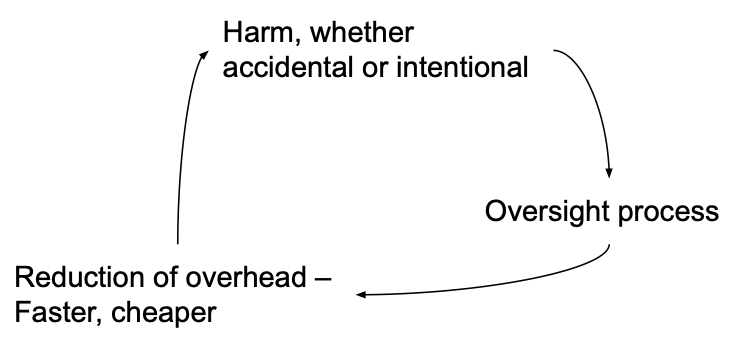
\includegraphics{images/process_loop_harm-oversight-improvement}
    \caption{The harm-oversight-improvement loop that motivates policies and processes.}
    \label{fig:harm-oversight-improvement}
\end{figure}







% Process discovery: Detect whether a process exists. 

% https://graphthinking.blogspot.com/2015/07/notes-on-bureaucracy-and-social-network.html
%Do participants know about existing processes?

%Processes can be undocumented. Then oral folklore is the mechanism. 

 \clearpage
    \section{Why do Processes Exist?\label{sec:why-processes-exist}}


The following sections explain why organizations rely on \glspl{process}. The reasoning matters to you in your role as a bureaucrat when you design a process or try to revise an existing process. Similarly, as a person going through a process, the reasoning below explains why you are experiencing \gls{process friction}. 

\subsection*{Processes Enable Consistent Application of Policy}

Organizations are intended to be insensitive to individual participants. That de-personalization applies to both bureaucrats and subjects. In practice there is sensitivity to who the bureaucrat is and who the subject is. 

Processes address risk to the allocated resource and risk to the bureaucrats carrying out the process.
Use of processes address the risk of both current bad behavior and the potential of things going bad in the future. Process is the guardrail limiting harm to bureaucrats and the shared resource. 

One motive for bureaucracy is the \href{https://en.wikipedia.org/wiki/Tragedy_of_the_commons}{Tragedy of the commons}, 
\index{Wikipedia!\href{https://en.wikipedia.org/wiki/Tragedy_of_the_commons}{Tragedy of the Commons}}
which says that when there is a shared resource someone will try to get away with behavior that is harmful to the community of users. Limiting harmful behavior can take the form of oversight processes. If oversight processes are not in place malicious actors dominate.

Another example guardrail is keeping stakeholders informed (justifications) so that intervention can be taken if needed. 

Each process for oversight, review, or approval may be justifiable when evaluated in isolation, but the aggregate can feel unreasonably burdensome to both subjects and bureaucrats.


% https://advancedbiofuelsusa.info/rodney-hailey-sentenced-to-more-than-12-years-in-prison-for-selling-9-million-in-fraudulent-renewable-fuel-credits/



\subsection*{Processes Enable Simplification}
Compared to an ad hoc approach, processes are intended to simplify what could otherwise be complicated moral decisions, complex coordination challenges, or financial assessments. %The simplification benefits the bureaucrat's workload; rarely are benefits to the subjects of the bureaucracy.  


The relation between complexity of a task and skill of the bureaucratic workforce is another motive for the creation of processes.
A positive story is that specialization allows narrow focus and thus deeper understanding and skill. An alternative perspective is that specialization allows for dumbing down the role, thus enabling a cheaper workforce. See figure~\ref{fig:complexity-and-size} 
\ifhaspagenumbers
on page~\pageref{fig:complexity-and-size} 
\fi
for a visualization of the trade-off.

Applying a process allows dumb individuals to do complicated things. The collective talent exceeds that of any individual.  As a specific example, consider the process of designing and building a car. That complexity is feasible to undertake for a skilled and knowledgeable individual, but the cheaper approach is to hire individuals capable of installing the passenger-side doors in an assembly line.

% Potential story to inject: founders of AMD left Fairchild
% https://en.wikipedia.org/wiki/Advanced_Micro_Devices#History

\subsection*{Processes Enable Increased Throughput}

Processes that leverage specialization can improve scalability. Adam Smith's \href{https://en.wikipedia.org/wiki/Business_process#Adam_Smith}{pin factory example} cites a productivity gain of 240x.
\index{Wikipedia!\href{https://en.wikipedia.org/wiki/Business_process}{Business process}}
Similarly, the introduction of moving assembly lines in Ford's car factory produced an 8x improvement of throughput \footnote{Wikipedia entry describing \href{https://en.wikipedia.org/wiki/Assembly_line\%2320th_century}{Ford's assembly line}
\index{Wikipedia!\href{https://en.wikipedia.org/wiki/Assembly_line\%2320th_century}{Assembly line}}
}. 


While social processes may work well for low-volume ad-hoc requests, formalized bureaucratic processes become necessary for recurring high-volume activities.

\subsection*{Processes Enable less Reliance on Social Relations}

The relation between bureaucratic processes and social bonds was noted by Selznick in his 1943 paper~\cite{1943_Selznick}. The needs of individual members of an organization may be at odds with (or at least not aligned with) the purpose of the organization. This dissonance is observed as the interplay between personal relationships and bureaucratic processes.

Generalizing claims about social bonds in an organization is unfounded. 
For a given complexity and given scale, there are people who are more social and less social and therefore desire more or less process.
There are bureaucrats who want documented processes and are confused as to how things are operating when those aren't present. 

The invisibility of social relationships limits bureaucrats not attuned to the importance of these bonds. 
Social influence among bureaucrats lacks transparency-- discoverability and documentation. 
In contrast, processes are easier to understand and to track. The counter to social influence is the hierarchical \gls{org chart} described on 
page~\pageref{sec:org-chart-as-guide-and-lie}.
Social influence is not antithetical to processes. There's always a mixture of the two.


\subsection*{Processes Enable New Bureaucrats and Subjects}

Bureaucrats new to a team are likely to ask, ``What are the processes and where is the documentation?'' Bureaucrats who have been on a team for a long time say, ``Don't burden me with processes, I just need to get things done using the relationships with the people I have.'' One motive for processes is to help with onboarding team members who don't have relationships available.

Besides not having formed a social network, there's a second reason new people seek processes. New team members who recently graduated from school are used to the existence of formal processes at the high school or university level. Therefore when they join a job, they expect a similar set of conditions for processes to exist and follow.

Once this motive for processes is recognized, the relevance when onboarding new hires is apparent. New hires will need to discover the existing processes while they form social bonds. Discovering processes comes through oral folklore or written documentation. To augment both process discovery and creation of relationship, one technique is to have new hires sit with experienced team members.
\marginpar{[Tag] Actionable Advice}
\index{actionable advice}
This is described in the section on  
\hyperref[sec:prisoner-exchange]{Prisoner exchange} on 
page~\pageref{sec:prisoner-exchange}.
Where you sit matters to your effectiveness as a bureaucrat.

\subsection*{Processes Enable Promotion}

Processes can arise organically (bottom up) or be created top-down. In either context, creating a new process counts as bureaucratic innovation. Process creation is confused as being worthy of promotion because of the lack of distinction between novelty and innovation. Real innovation incurs risk, whereas new processes are merely novel. Both cause change, but processes are typically designed to decrease risk. Rewarding decreased risk is reasonable, but it shouldn't be labeled as innovation.

 \clearpage
    \section{Riding the Chaos\label{sec:process-chaos}}

Bureaucratic organizations are imperfect because they are composed of humans. %Somethings work, others do not. 
A bureaucratic organization is a complex and chaotic\footnote{Chaotic in the \href{https://en.wikipedia.org/wiki/Chaos_theory}{mathematical sense} 
\index{Wikipedia!\href{https://en.wikipedia.org/wiki/Chaos_theory}{chaos theory}}
of non-linear dependence on initial conditions, not just colloquial sense of disorder} environment. An understandable response is to impose processes and hierarchy and roles. Imposing structure can feel intellectually fulfilling and emotionally satisfying. Imposing structure looks like progress and may even help with your promotion in the hierarchy. The challenge (or continual source of employment) is that chaos is dynamic. A process created in response to chaos create new challenges and is disrupted by changes in number of staff, changes to who is part of the process, changes to amount of work. The half-life of structure depends on the rate of change of tasking and the rate of 
\marginpar{See page~\pageref{sec:turnover}.}
\hyperref[sec:turnover]{personnel turn-over}\iftoggle{haspagenumbers}{; see page~\pageref{sec:turnover}.}{.}

A bureaucrat in the organization could strive for perfection, run away from the chaos (to something less chaotic), exploit the chaos, or adopt an attitude of ``I do what I can'' or ``I'll wait out the problem.'' 
Another option, and the focus of this section, is to build skills for navigating the chaos of a bureaucratic organization.

You can build and maintain your network of professionally connections with fellow bureaucrats. 
\marginpar{$>>$ Actionable Advice} 
\index{actionable advice}
This augments the chain of command of a hierarchy. There is a turn-over in both hierarchical roles and in your professional network, so you need to continually invest effort in creating new bonds and maintain existing relations. 

You can see change as an opportunity for improvement rather than a destruction of your previous investments. The \href{https://en.wikipedia.org/wiki/Sunk_cost}{sunk cost fallacy}
\index{Wikipedia!\href{https://en.wikipedia.org/wiki/Sunk_cost}{sunk cost fallacy}}
applies both to your emotional state and the resources you invested. Fear of change is understandable -- it disrupts the comfort of stability and known processes. Anticipating change and preparing for it eases the stress of change.

You can leverage personalities and unique traits rather than expecting everyone to be interchangeable and treating differences as flaws. 
\marginpar{$>>$ Actionable Advice}
\index{actionable advice}
By knowing the strengths, interests, and weaknesses of coworkers you can facilitate the process of change.  \clearpage
    \section{Processes Involve a Person New to the Process}

% https://graphthinking.blogspot.com/2022/07/bureaucratic-processes-typically.html

% The IPYNB notebook is in
% https://drive.google.com/drive/u/0/folders/1awZYk4EisFIR3mY1iF2X7Hb6CwcNDavp

Bureaucratic processes require working with other people. One source of friction is that participants may lack familiarity with the process. 

This observation can be quantified with a small number of assumptions. The distribution of team membership tenure might fit a \href{https://en.wikipedia.org/wiki/Power_law}{power law distribution}
\index{Wikipedia!\href{https://en.wikipedia.org/wiki/Power_law}{power law}}\footnote{See \href{https://numpy.org/doc/stable/reference/random/generated/numpy.random.power.html}{numpy.random.power} documented on https://numpy.org/doc.}
-- there are more inexperienced people than experienced people. What matters in this context is how long the team member has been in their role (rather than how long they've been a member of the organization). Let's assume a max tenure of ten years~\cite{2022_BLS_tenure}. If the process involves five people, the least experienced member will have a median of 100 calendar days of experience.

% image float options:
% https://tex.stackexchange.com/a/32605/235813
\begin{figure}[!htb] %[H]
    \centering
    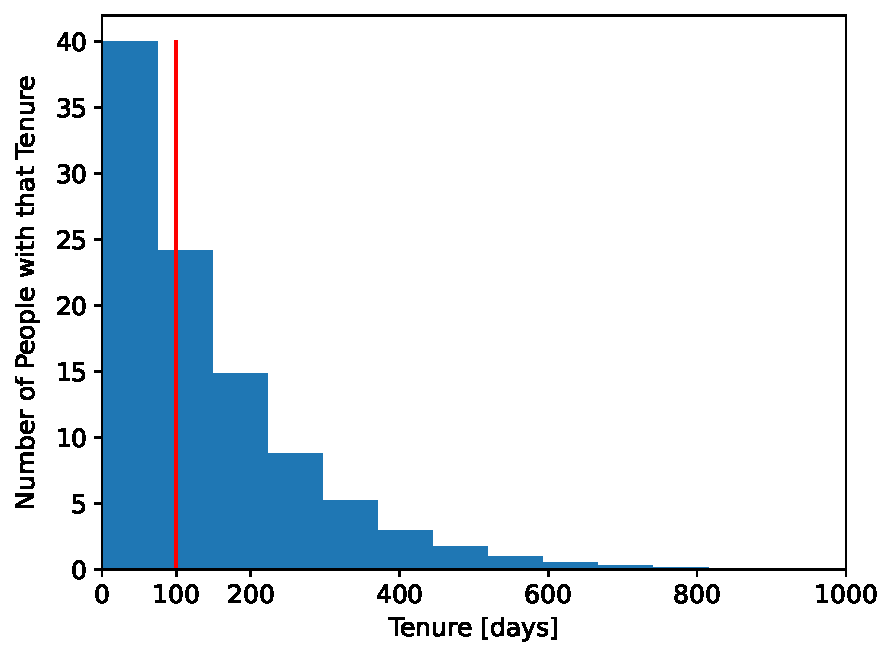
\includegraphics[width=0.8\textwidth]{images/tenure_power_distribution_a5_with_max_tenure10_and_5_participants.pdf}
    \caption{The power law distribution of tenure using the \href{https://en.wikipedia.org/wiki/Probability_density_function}{probability density function}
    \index{Wikipedia!\href{https://en.wikipedia.org/wiki/Probability_density_function}{probability density function}}
    described by $a\ x^{(a-1)}$ where $a=5$. The median tenure of the youngest participant  in a process with five people is 100 days. Population size has been normalized to 100 people.}
    \label{fig:tenure-powerlaw-5-participants-tenure10}
\end{figure}


Three calendar months (or 70 business days) may be inadequate for complex processes or processes that are infrequent (quarterly or annual), especially if there was no training. When the number of participants is ten people, then the median tenure of the youngest participant is 51 calendar days (37 business days).

\ \\

To recap, the assumption made were:
\begin{itemize}
    \item Random, independent sampling of organization members. 
    \item Tenure in your role matters, not the tenure in the organization. (This assumption excludes transfer learning among roles.)
    \item Tenure in role fits a power law distribution.
    \item The power law distribution is characterized by (a=5, max tenure=10 years). 
    \item There are five people involved in the process.
\end{itemize}
If that last parameter is varied, the estimate of three months as the median  is reasonable for processes with five or more participants.

% image float options:
% https://tex.stackexchange.com/a/32605/235813
\begin{figure}[!htb]  %[H]
    \centering
    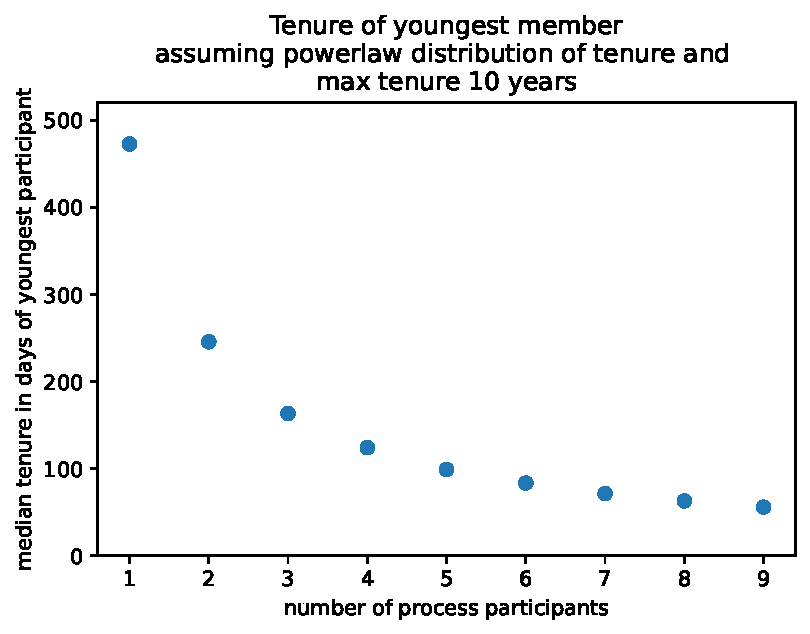
\includegraphics[width=0.8\textwidth]{images/tenure_power_distribution_a5_with_max_tenure10.pdf}
    \caption{Median tenure of the youngest participant (in calendar days) as a function of the number of process participants with tenure following a 
    \href{https://en.wikipedia.org/wiki/Probability_density_function}{probability density function},
    \index{Wikipedia!\href{https://en.wikipedia.org/wiki/Probability_density_function}{probability density function}}
    $a=5$, and max tenure of ten years.}
    \label{fig:tenure-powerlaw-5-participants}
\end{figure}


Even when there's a single participant, the median tenure is less than two years because of the power law distribution of tenure.

% Uniform Distribution of Tenure instead of a Power Law Distribution
What if the power law distribution of tenure were replaced with a uniform distribution?
Surprisingly the shape of the distribution of the youngest participant's tenure is not uniform, see Figure~\ref{fig:tenure-uniform-5-participants}

% image float options:
% https://tex.stackexchange.com/a/32605/235813
\begin{figure}[!htb]  %[H]
    \centering
    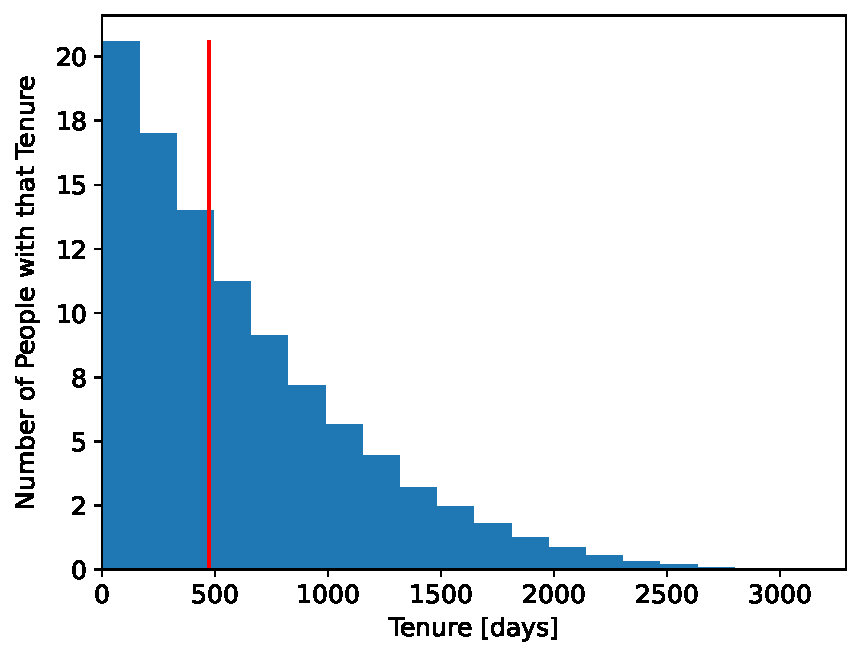
\includegraphics[width=0.8\textwidth]{images/tenure_uniform_distribution_with_max_tenure10_and_5_participants_median472.pdf}
    \caption{The median tenure of the youngest participant
 in a process with five people is 472 days when the distribution of tenure is uniform. The population size has been normalized to 100 people.}
    \label{fig:tenure-uniform-5-participants}
\end{figure}

The median tenure of the youngest member of a process with five participants is 15 months. 

% https://latex.org/forum/viewtopic.php?t=17111
\FloatBarrier \clearpage
    \section{Automating Processes\label{sec:automating-processes}}



% https://graphthinking.blogspot.com/2022/07/automating-management.html

For bureaucratic organizations that deal with intangibles (referred to as ``\href{https://en.wikipedia.org/wiki/Knowledge_worker}{knowledge work}''), the desire to automate processes is wide-pread.  (When physical objects are involved, then robotics is necessary for automation.) Automation has the benefits of consistency, predictability, decreased labor costs, and easier troubleshooting. 

% why automation doesn't happen by default:
While the benefits of automation are known to participants, there are barriers to automation you will need to address.  
As with making information discoverable and searchable, automation requires an investment of time, money, and skills that are ancillary to the purpose of the organization. A transition from manual processes to automated workflows requires doing the original work while enabling automation. Creating the conditions that are needed for automation has a delayed pay-off. 

The evolution of automating a process involves
\begin{enumerate}
    \item Identify who is involved in the process. How did the process get created and how has it evolved up to now? Who evaluates the success of the process? 
    \item For existing processes, transition verbal folklore to written documentation. The purpose of this step is to write down the workflow, business logic, and relevant decisions. 
    \item Transition the documentation in the previous step from plain text documentation to structured data. Examples of structured text that can be parsed by a computer include  decision trees and workflow diagrams. Implementation could be in \index{Wikipedia!Graphviz@\href{https://en.wikipedia.org/wiki/Graphviz}{Graphviz}}
    \href{https://en.wikipedia.org/wiki/Graphviz}{Graphviz} or \index{Wikipedia!PowerPoint@\href{https://en.wikipedia.org/wiki/Microsoft_PowerPoint}{PowerPoint software}} \href{https://en.wikipedia.org/wiki/Microsoft_PowerPoint}{PowerPoint}.
    \item Collect metrics (for example, the number of times software application was opened, how frequently the folder was reviewed, how much  time was spent on the webpage) for existing manual processes to enable cost evaluation for implementing automation. This is the modern version of a
    \index{Wikipedia!time and motion study@\href{https://en.wikipedia.org/wiki/Time_and_motion_study}{time and motion study}}
    \href{https://en.wikipedia.org/wiki/Time_and_motion_study}{time and motion study}.\footnote{\href{https://xkcd.com/1205/}{https://xkcd.com/1205/} -- the trade-off of task frequency versus temporal savings per task instance.}
    \index{xkcd!xkcd.com/1205@\href{https://xkcd.com/1205/}{1205}}
    \item Implement stand-alone software (scripts) for each task using personal automation tools like \href{https://pyautogui.readthedocs.io/en/latest/}{PyAutoGUI} (a free Python-based automation package) or \href{https://www.autoitscript.com/site/}{AutoIt} (a free domain-specific language for Windows GUI applications).
    \item Tie the scripts in the previous step to the task workflows from step 2.
    \item Create an automation assistant that actively monitors your activities (keystrokes, mouse clicks, on-screen events) to detect repetitive actions that are candidates for automation.
\end{enumerate}

The path described above is not accessible to many bureaucrats for multiple reasons. 
The barriers to automating bureaucracy depend on having relevant skills, IT resources, and predictable workflows that justify the
\index{Wikipedia!return on investment@\href{https://en.wikipedia.org/wiki/Return_on_investment}{return on investment}}
\href{https://en.wikipedia.org/wiki/Return_on_investment}{return on investment}. Compounding these hurdles, the skill of identifying opportunities for automation depends on your practical skills (what are you capable of) and your experience.

Where you are in the hierarchy of your bureaucratic organization affects your options. 
Automating bureaucracy from the bottom-up can be augmented and supported by management. 
At the organizational level, there are system-level changes like
\begin{itemize}
    \item Hire people who desire automation and the skills to enact automation.
    \item Use tracking bits in
    \index{Wikipedia!PDF@\href{https://en.wikipedia.org/wiki/PDF}{PDF}}
    \href{https://en.wikipedia.org/wiki/PDF}{PDFs} and webpages to collect data on how systems are used. This decreases the burden on process participants to report metrics and can be less biased since it does not rely on self-reporting.
    \item Provide a metrics aggregation service. The ability to store metrics from multiple teams enables a holistic perspective on the organization and can help identify chokepoints. Without the ability to view the entire organization, premature optimization is likely.
    \item Align incentives (e.g., pay, promotion) with the implementation of automation.
    \item Transition from paper to 
    \href{https://en.wikipedia.org/wiki/PDF}{PDF} 
    \index{Wikipedia!PDF@\href{https://en.wikipedia.org/wiki/PDF}{PDF}}
    to a website to an%
    \index{Wikipedia!API@\href{https://en.wikipedia.org/wiki/API}{API}}
    \href{https://en.wikipedia.org/wiki/API}{API} (application programming interface).\footnote{To read about how this worked out at Amazon, see \href{https://gist.github.com/bhpayne/49c8379a3ea880b7cc079fc8d32c87a7}{Yegge's 2011 description}~\cite{2011_Yegge}.}
%and \href{https://news.ycombinator.com/item?id=3101876}{https://news.ycombinator.com/item?id=3101876}}
%and \href{https://news.ycombinator.com/item?id=27566676}{https://news.ycombinator.com/item?id=27566676}.}
    \item Members of bureaucratic teams should be trained to develop software, share code, use \href{https://en.wikipedia.org/wiki/API}{API}s, 
    \index{Wikipedia!API@\href{https://en.wikipedia.org/wiki/API}{API}}
    create APIs, and maintain APIs.
\end{itemize}

%\ \\

%\noindent\hrulefill

Automation can reduce labor costs, but designing, implementing, maintaining, and updating automation requires significant investment, a change of culture, and new skills for the workforce.  


% TRANSITION to next section: process_exceptions
When automating bureaucratic processes, exceptions disrupt the expected workflow of tasks that comprise the process. Handling exceptions is a tricky subjective topic because exceptions are sometimes critical to allow for and can be abused. Abuse of exceptions to a process can originate from the subjects of a process or from the bureaucrats administering the process. \clearpage
    \section{Exceptions to a Process\label{sec:exceptions-to-process}}


Process designers are usually motivated to address a specific issue associated with access to shared resources. When bureaucrats execute a process to support a policy, there may be cases that violate the designer's assumptions. Now the person with the exceptional case and the bureaucrat carrying out the policy have extra work to deal with the broken process. This is a source of \hyperref[sec:bureaucratic-debt]{bureaucratic debt}. 
\marginpar{See page~\pageref{sec:bureaucratic-debt}.}
%\ifsectionref
%(see section~\ref{sec:bureaucratic-debt} for details). 
%\fi

When the routine process is inadequate, there are routes for exceptions:
\begin{itemize}
    \item Change the process to address the exceptional case. This takes extra time and work for the subject and the bureaucrat.
    \item Ignore the process. Use relationships instead.
    \item Ignore the task. If the result wasn't crucial to your efforts and the work is too burdensome compared to alternatives, terminate the process.
    \item Seek an exception to the process. The exception can be recurring or one-time. The justification for the exception can be based on social capital of participants (title, reputation) or be a data-driven argument or some mixture of both.
\end{itemize}

The designer of a process may not be able to anticipate future circumstances, but expecting the capacity to be responsive to change is reasonable. The process designer should use sunset provisions and escape hatches.  
\marginpar{$>>$ Actionable Advice}
\index{actionable advice}
A sunset provision can be time-based (this policy expires after 3 years) or based on a threshold (this policy should be evaluated for renewal after 1000 cases). An escape hatch specifies the conditions under which the participants are excepted from the policy. A good escape hatch for a policy provides directions about what follow-on actions should be taken.

Another reason processes may be inadequate is due to urgency. A result that is needed quickly may not fit the timeline of sequential tasks for a process.

\subsection*{Time Sensitivity Exceptions}
Exceptions to a process may be required when a result is need quickly. In the medical setting there are categories of urgency; a task may be routine, priority, urgent, stat. 
Each of those categories is associated with a time bound, though the specific duration varies by medical domain and by location.\footnote{\href{http://docport.columbia-stmarys.org/EHR/PhysicianOrdersPriorityandDeptServiceHours.aspx}{Physician Orders Priority} and \href{https://www.unitypoint.org/peoria/services-priority-definitions-and-critical-values.aspx}{Priority Definitions}}
% as of 2022-12-17, the docport.columbia-stmarys.org page is unavailable. The google cache and Wayback machine provide valid pages.

Common failure modes for processes include abuse of prioritization (everything is important) or abuse of urgency (everything is needed quickly). Either of these abuses need to be corrected to have a healthy bureaucracy, but typically the cost of labeling an effort as ``priority'' or ``urgent'' is low. 

To limit abuse of processes, interaction between the bureaucrats tasked with work and the people characterizing relative value is needed. This interaction is a negotiation of what work gets done when and in what order. Labeling every task as ``urgent'' is a failure to communicate the relative value of a set of tasks.


Process friction can arise from the separation of roles needed to support a process. Those separate roles can happen within a team of bureaucrats, or the process can span distinct teams. The difficulty imposed across teams within an organization is moderated by the existence of a common arbiter in the chain of command.  
% TRANSITION to next section: processes_two
Troubleshooting processes is even more complicated when processes span organizations.   \clearpage
    \section{Processes involving Two Organizations\label{sec:processes-two-organizations}}

When two independently-managed processes interact across organizational boundaries there can be friction. Process friction, especially between two  organizations that lack shared coordination, results in either \hyperref[sec:exceptions-to-process]{exceptions to the process} 
%\ifsectionref
%(section~\ref{sec:exceptions-to-process}) 
%\fi
or lying or a \hyperref[sec:change-a-process]{change in process}.
%TODO \marginpar
%\ifsectionref
%(section~\ref{sec:change-a-process}). 
%\fi

The following stories illustrate process friction between teams within an organization and process friction between organizations. The teams within an organization have shared objectives (set by the organization), whereas separate organizations lack incentive to coordinate. 

\subsection*{Data Transfer from one Team to Another}

\marginpar{[Tag] Story Time}
\index{story time!data transfer}
\begin{mdframed}
Two teams in an organization have a relationship, and each has data storage and data processing capability. Allen's team sends Bob's team data on a weekly basis. Because the teams were built for different purposes and at different times by different people, the data storage capabilities used by each team are not compatible. Members of Allen's team print all the records (usually about a hundred pages) and then delivers the paper documents to Bob's team. Members of Bob's team then retype all the information into the data storage used by Bob's team.

Recently the office went paperless. Now Allen's team sends Bob's team a set of PDF files. Member's of Bob's team type in the content from the PDFs into the database for Bob's team. This is deemed a win for efficiency -- no more printing of paper documents each week!

\ \\

Why doesn't the organization common to both teams hire a data scientist to automate the recurring data transfer? Or train the current staff to learn to program a solution? Or create a third team that manages a common server?

Because the current staff skill set supports printing and typing (data entry). Training someone with a new skill set takes an investment of money, time, is an opportunity cost, and makes them a flight risk.
Hiring a data scientist is expensive. Whether the task is feasible is uncertain from the view of Bob and his manager (they both lack experience with the needed technology), and how long the task will take is uncertain. Even once they create a connection, then a person with the skill set to maintain it is needed. The cost of ongoing maintenance and implementation is unknown.

Known working suboptimal with known cost versus unknown potential improvement of unknown degree for an unknown capital and ongoing cost. And if that improvement works out, staff who were implementing the old solution now need to find new work.
\end{mdframed}

Two teams operating within an organization, with a shared intent and working relationship, may be stuck with the process they have even when the friction is clear. When organizations lack a common objective, the friction can be even more significant. 

\subsection*{Example of coordinating processes between two Organizations}
This story is about receipts from one process being submitted for reimbursement to another process.
Submitting the receipt shifts the accountability and justification burden to the accepting bureaucrat.

% https://graphthinking.blogspot.com/2017/02/financial-motivation-in-bureaucracy.html
\marginpar{[Tag] Story Time}
\index{story time!dental insurance}
\begin{mdframed}
I have dental insurance. I visited the dentist December 2 and one of the procedures during a routine cleaning was ``bitewing x-rays." This procedure is covered by my insurance, so I was surprised when I received a bill for it from my dentist a few weeks after my visit.

I called my dentist and they explained that the dental insurance had declined to pay for the procedure. I called the insurance company January 3 and they confirmed that the procedure was covered by my policy. 
Every time I call the insurance provider I had to provide my social security number, date of birth, and zip code twice -- once to the automated system, a second time to the person I talk with. The insurance company apparently had made a mistake and said they would cover the cost of the procedure. I followed up with my dentist and explained the situation.

I called the dentist to see if they had received payment yet. They had not, so I called the dental insurance provider again February 6 and 8. February 8 the insurance company said they would process the payment within 7-10 business days. I called again February 20 and the claim hadn't been started within the insurance company. I spoke to the supervisor and she said she would personally visit the claims office within the insurance company.

From the perspective of the dentist, they are seeking money for the service they provided me.

From the perspective of the insurance company, delaying payment on a claim makes good financial sense -- the policy holder is likely to just pay the balance to avoid going to court with the dentist.

From my perspective, the question is whether chasing this issue makes financial sense. I think of my hourly rate as \$40, so after an hour the charge of \$38 would have been better to pay out of pocket. Effectively I'm devaluing my time. The emotional stress and thought-cycles spent are also relevant, though harder to quantify.

Streamlining bureaucratic processes does not occur automatically. There needs to be both incentive to change and authority to make the change. 
\end{mdframed}

In the above story the dental office wanted to be paid for services provided. The insurance company wanted to minimize the number of payments made. And I wanted to minimize my costs. While none of those are conflicting, each organization has separate objectives.

\subsection*{Deploying Bureaucrats to Different Teams or Organizations\label{sec:prisoner-exchange}}

One method of addressing friction between teams or organizations is to deploy a person. This may not result in a specific change, but it can help members of both the originating team and receiving team better understand their counterpart. For the rest of this section I'll use ``team~A" as the origin and ``team~B'' as the receiver, though the concept applies to exchange of organization members. The name of the bureaucrat in this example is Mark. This example covers an informal deployment in which Mark remains employed with team~A. While Mark is with team~B he provides the management of team~A with a weekly activity report. 

The easiest question regarding Mark's deployment to team~B is ``how long?'' That depends on the purpose of the exercise and the complexity of the work Mark will be doing with team~B, as well as how long team~A can operate without Mark's contributions. What is a successful outcome for Mark? For team~A? For team~B? For the organization? How long will integration of Mark onto team~B take? Does Mark need time on team~A to delegate current work?

A deployment harms the productivity of originating team~A by loss of staff. The deployment also harms Mark's productivity for his work with team~A. The deployment harms the receiving team~B since they have to train or integrate Mark. 

Incentives for this investment include cross-training for Mark, better process empathy for both teams, and temporary (exceptional) support. What is team~B expecting from Mark? How will team~A benefit? What is Mark expecting to gain from the deployment? Or is this a sacrifice on Mark's part? 

Cross-training Mark can improve productivity of Mark and the teams. 
team~B gets to hear an outsider's perspective from Mark, and Mark returns to team~A with a broader perspective of the organization.
A deployment can build relationships among the teams. Both teams are better able to address process friction or exceptional interactions. 


Potential engagement modes for Mark: consultant (providing knowledge to team~B), integree (increasing the capacity of team~B), or shadowing (learning from team~B). Shadowing can be of an individual on team~B, or Mark can shadow team~B by attending meetings. 


Mark could be deployed full time for the entire duration, split his him between teams, or build-up and back-down over the course of the deployment.

Are there criteria for early termination of the deployment? Are there criteria for extending Mark's deployment?

If this sounds useful to your team there are a few considerations. Are you on the originating team A or the receiving team B? Who gets deployed? How is Mark picked? Was the opportunity advertised? If you're receiving Mark, what are your acceptance criteria? How many concurrent deployments can your team support?


\subsection*{Service-Level Agreements\label{sec:sla}}

When two teams or two organizations need to interact on a recurring basis, a formalized approach is to create a \href{https://en.wikipedia.org/wiki/Service-level_agreement}{Service-Level Agreement}. 
\index{Wikipedia!\href{https://en.wikipedia.org/wiki/Service-level_agreement}{Service-Level Agreement}} 
While a Service-Level Agreement (SLA) is constructive for outlining what each party expects from the other, within a bureaucracy an SLA is typically not a legally binding contractual agreement. Instead of a judge resolving disputes, an SLA within a bureaucracy may be adjudicated by a supervisor common to the two teams.

A Service-Level Agreement within a bureaucracy is dependent on the good will and honor of the signatories. Since an SLA is a formalization of a relationship, it is subject to revision when there is turn-over of signatories in any of the teams. 

An Service-Level Agreement should include providing historical and live data to stakeholders so violations can be measured. The need for measurements is because enforcement of the SLA is by the signatories. Observability is key to accountability. 

A supervisor common to the parties may be invoked when an SLA is not met, or if there is a dispute over the interpretation of an SLA. Usually the threat of invoking oversight is enough to coerce change in negotiations. 
When the common supervisor gets involved there are not many options available for sanctions. The supervisor could withhold bonuses or promotions, or assign a new team lead, or re-negotiate the SLA. 

Because creation of SLAs are burdensome to all parties invovled, monitoring to enable enforcement incurs work, and punishment is limited, most cooperation between teams and between organizations is informal and ad hoc. Relying on personal relationships is easier than formal agreements. Reputations, both for individual bureaucrats and for teams and organizations, are then formed on the basis of performance and reliability.

\ \\

% TRANSITION to next section: process_mistakes
%TODO
The next section addresses mistakes, a common source of process friction. 
 \clearpage
    \section{Process Mistakes\label{sec:process-mistakes}}

Any process involving humans incurs mistakes
\footnote{\href{https://en.wikipedia.org/wiki/Murphy\%27s_law}{Muphy's law}
\index{Wikipedia!\href{https://en.wikipedia.org/wiki/Murphy\%27s_law}{Muphy's law}}
}. The only way to drive the number of mistakes to zero is by doing nothing, but that isn't a practical way of managing shared resources. 
The purpose of pondering bureaucratic mistakes is to come up with ways to limit the consequence of mistakes to cause damage. 

\subsection*{Fixes are Difficult}
Imposing checks on a process as a way to  reduce mistakes creates more bureaucracy. The extra work can be in the form of redundant data collection, or additional justifications needed. 
Maintaining coordination of diverse activities in a bureaucracy requires that information propagate up the chain of command to a common authority. Some mistakes like duplication of effort can only be detected by checks made high up the chain of command.


\subsection*{Fixes Fail}
The path of information from the person with a problem to the person who can address the situation may pass through many people. 

The consequence is familiar to people who have played the \href{https://en.wikipedia.org/wiki/Chinese_whispers\%23Game}{game of telephone}.
\index{Wikipedia!\href{https://en.wikipedia.org/wiki/Chinese_whispers\%23Game}{game of telephone}}
%\marginpar{[Tag] Story Time}
\index{story time!game of telelphone}
\begin{storytime}{Game of Telephone}
The person has a problem and explains their problem to the helpdesk staff member. The helpdesk staff member hears the problem with incomplete context and from their own frame, then relays it to their manager, who talks to the manager of the engineering team, who delegates the responsibility to the engineer. 
\end{storytime}
This is a solvable problem: the engineer could talk with the customer. 
% source: 
% https://news.ycombinator.com/item?id=30480083

At each hand-off there is a significant chance the information is unintentionally mangled. 

\subsection*{Where Process Mistakes come from}
Mistakes in a process can originate from the bureaucrat who inflicts the process, in the hand off between participants, or from the \gls{subject} of the bureaucratic process. Typically there are more checks on subjects and fewer on bureaucrats. 

\subsection*{Choices about Mistakes}
As a process participant, I may cause a mistake or observe a mistake. My options are to can ignore it, fix it (which incurs extra work), or report it. If I chose to report it, I can do so anonymously (which decreases the risk of harm to my reputation, but also eliminates feedback) or with my name so that discussion can occur and I get feedback.

\ \\

\noindent\hrulefill

\ \\

% TRANSITION to next section: process_design_of
Pondering types of mistakes and causes of mistakes for processes is important if you want to revise a process or create a new process. \clearpage
    \section{Design of Processes\label{sec:design-of-processes}}

TODO: where does this fit in?

Deployment of processes need to account for 
normal users, power users, malicious users, and edge cases.

\ \\


TODO: where does this fit in?

% https://graphthinking.blogspot.com/2016/04/if-you-want-boulder-to-roll-place-it-at.html
When designing a process, look for ways to minimize the work for people involved. Minimizing work (both physical and mental) for the people involved means less sensitivity to entropy in a bureaucracy. Minimizing work requires significant situational awareness on the part of the designer. To minimize effect on existing bureaucracy, it's vital to minimize the requirements to achieve success.

\ \\


Bureaucracy is the use of distributed knowledge and distributed decision making for policies concerning access to shared resources. A set of \glspl{process} is used by \glspl{bureaucrat} to leverage specialization and improve throughput. 
    
Because bureaucrats are typically not formally trained in designing processes, ad hoc ideas reactive to the immediate situation and local constraints are used. A thoughtful process designer attempts to account for exceptions (page~\pageref{sec:exceptions-to-process}) and potential mistakes (page~\pageref{sec:process-mistakes}).

The following sections describe why static process designs are the norm, the role of bureaucratic debt, and how to design for turnover of staff.
    
\subsection*{Static and Dynamic Process\label{sec:static-dynamic-processes}}

% https://graphthinking.blogspot.com/2017/04/static-versus-dynamic-processes.html

Change within an \gls{organization} \iftoggle{glossaryinmargin}{\marginpar{[Glossary]}}{}%
is to be expected since the external environment the organization exists in is not static. 
Sources of external change include improving technology, changes to the \gls{shared resource}, \iftoggle{glossaryinmargin}{\marginpar{[Glossary]}}{}%
or shifting expectations of subjects of the bureaucracy.
Change is also driven internally to the organization by \hyperref[sec:turnover]{turnover of staff}.%
\marginpar{See page~\pageref{sec:turnover}.}
Since change is expected, why are static processes that are not robust to change created in the first place? Because static processes are easier to design and appear initially to require less maintenance.

Creating robust processes that are dynamic takes more effort to create. First, the process must be documented so that it can be analyzed. What is expected to happen? Who are the stakeholders? These conditions are likely to change, making the process fragile. Second, document assumptions used in the process. If the assumptions are invalidated, then the process is broken and needs to be discarded or at least revised. 

A challenge is that even when the process is documented and assumptions enumerated, there may not be an incentive to check to see if revision is necessary. Measurements (which are costly and disruptive) need to be periodically taken to see if the assumptions are still applicable. To force periodic validation of assumptions, one approach is to use \href{https://en.wikipedia.org/wiki/Sunset_provision}{sunset provisions} -- automatic expiration dates set at the time of creation. 
\index{Wikipedia!sunset provisions@\href{https://en.wikipedia.org/wiki/Sunset_provision}{sunset provisions}}
\iftoggle{WPinmargin}{\marginpar{$>$Wikipedia: sunset provisions}}{}

A more quantitative approach (and even less frequently used) is to tie a process to a cost-benefit model. Enacting a process provides a benefit and comes at some cost. If the assumptions of the process can be tied to a cost-benefit model, then we can determine whether the process is worth enacting. Periodic measurements are needed to update the cost-benefit model and determine whether the process is effective.

Summarizing the steps for creating a robust process,
\begin{enumerate}
    %\item If a process already exists, document the process that is fragile.
    \item List assumptions used in the process. Who are the stakeholders, what are the goals, and what are the constraints?
    \item Relate the assumptions to a \href{https://en.wikipedia.org/wiki/Cost\%E2\%80\%93benefit_analysis}{cost-benefit model}.
    \index{Wikipedia!cost-benefit model@\href{https://en.wikipedia.org/wiki/Cost\%E2\%80\%93benefit_analysis}{cost-benefit model}}
    \iftoggle{WPinmargin}{\marginpar{$>$Wikipedia: cost-benefit model}}{}
    \item Determine the measurable parameters of the cost-benefit model. 
    \item Collect recurring measurements to verify the assumptions. 
    \item If the assumptions are broken, revise the process. 
\end{enumerate}
A robust process is just a fragile process with a feedback loop informed by ongoing measurements. Robust processes require extra work by bureaucrats compared to static processes. A static process shifts the burden to subjects. In this situation bureaucrats have externalized the burden.
In practice, ignoring exceptions and reacting to problems is common because then there's less work for the bureaucrats enacting the process. Process Empathy in this case is not just rationalizing suboptimal behavior, but empowers you to take action. 

\ \\

The above description of robust dynamic processes and fragile static processes characterizes workflows in isolation from the history of a team or organization. Typically processes are evolved from previous processes.  That evolution induces another source of bureaucratic friction. 

\subsection*{Decisions and Processes Create Bureaucratic Debt\label{sec:bureaucratic-debt}}

% https://graphthinking.blogspot.com/2017/09/bureaucratic-debt-and-what-to-do-about.html

Suppose a \gls{process} is enacted and later found to be ineffective. Some work is needed to revise the process and hopefully improve effectiveness (or an \hyperref[sec:exceptions-to-process]{exception} is needed).
%\ifsectionref
%; see section~\ref{sec:exceptions-to-process}).
%\fi
\iftoggle{glossarysubstitutionworks}{\Gls{bureaucratic debt}}{Bureaucratic debt}\footnote{Similar to the concept of \href{https://en.wikipedia.org/wiki/Technical_debt}{technical debt} in the creation and maintenance of software\iftoggle{printedonpaper}{; see Wikipedia entry}{}.
% 2023-11-15: the "\index" on the next line has to have a line break, or else pandoc's parser gets confused
\index{Wikipedia!\href{https://en.wikipedia.org/wiki/Technical_debt}{technical debt}}} is 
\iftoggle{glossaryinmargin}{\marginpar{[Glossary]}}{}  the work needed to change a process.
Bureaucratic debt is caused by choosing an easy solution now (with limited information or insufficient resources) instead of using an approach that would take longer to design and enact but be more robust.


Decisions made by \glspl{bureaucrat} occur in a resource-constrained environment.
Getting information (measurement) and analysis are costly in terms of money, time, skill, and labor.
Each decision made results in options that are not explored. These missed opportunities are associated with short-term versus long-term trade-offs of costs.

The \href{https://en.wikipedia.org/wiki/Opportunity_cost}{opportunity costs}
\index{Wikipedia!\href{https://en.wikipedia.org/wiki/Opportunity_cost}{opportunity cost}}
(options the organization doesn't take) alter which future decisions become available.

\ \\

The purpose of defining bureaucratic debt as a concept is to capture the work resulting from decisions that would otherwise be unaccounted for.
Once the concept of bureaucratic debt is understood it can be tracked.

To document bureaucratic debt, you need to record aspects of decisions as they are made:
\begin{itemize}
    \item What is the decision to be made?
    \item When was the decision  identified?
    \item When was the decision made?
    \item Who made the decision?
    \item What options were identified?
    \item Which option was chosen?
    \item Why was that option  chosen over the other options?
\end{itemize}
The purpose of documenting decisions is to enable both aversion to bad decisions and attraction to good decisions. That may sound strange, but the default of decision-makers is to apply the same behavior in future decisions. 
Without documenting decisions, there is no transparency, accountability, historical measure of progress, or ability to track dependencies. 

Creating a record of decisions is necessary but not sufficient. The documentation of decisions needs to be shared with stakeholders to enable accountability. This should occur as promptly as possible. 

Every bureaucrat exercises policies that apply to subjects, even if the subjects are other bureaucrats. What I'm describing above is beyond merely documenting what the processes and policies are for subjects. Documenting bureaucratic debt is for use internal to the team or organization.  

The scale of decision impact determines the level of documentation. ``Do I choose pencil or pen?" incurs negligible bureaucratic debt; therefore the documentation needed is also negligible. Projecting then consequence of decisions is a subjective prediction. 

%Similarities of tech debt and bureaucratic debt.
%In developing software, there are three artifacts: the software, documentation on how to use the software, and documentation on why to use the software. The two distinct types of documentation are typically combined in one document. Each of these three artifacts are independent. The ramification of this is that each artifact can be created independently, and it takes work to maintain synchronization of the artifacts. 



\subsection*{Design Processes for Turnover of Staff\label{sec:turnover}}

% https://graphthinking.blogspot.com/2020/02/design-for-turnover-rather-than-rely-on.html

When designing a \gls{process}, there are a few goals to optimize for: time-to-first-result, average latency, initial financial cost, total financial cost, flexibility to input conditions, throughput, and scalability. In theory all these factors should inform decision-making. An often neglected aspect that is harder to predict and harder to measure is the importance of employee turnover. 
On a long time scale, the turnover of \iftoggle{glossarysubstitutionworks}{\glspl{bureaucrat}}{bureaucrats} is 
a significant source of risk for any team or project. 

Besides the loss of knowledge associated with turnover, another complication is the change of assumptions when new people join an existing process. 
Processes are enacted differently than initially intended because the people implementing them are not the same people who came up with and designed them. One solution (rarely enacted) is to document the assumptions and reasoning for the design of a process. Having a written record enables bureaucrats who were not present at the time of conception to understand the purpose of the process. 

The conditions under which a process is created are not static -- requirements and resources change. 
Making processes resilient to change requires  bureaucrats to be educated beyond the requirements of the immediate task. The relevance of education is on-going: during onboarding of the bureaucrat, while carrying out the process, and as bureaucrats exit participation in the process. 

Providing training for a process is complicated by the variety of bureaucrats participating in a process.
That is why designing a process typically relies on roles -- participants are treated as interchangeable with other people who have similar skills. As a bureaucrat coming up with a novel process, accounting for differences in enthusiasm or communication among participants is difficult. 
Designing processes that are robust to turnover does not mean ignoring the unique talents of participants. 
To account for differences emphasize documentation that explains the how and why in training new participants. 
\marginpar{Actionable Advice}%
\index{actionable advice}


Onboarding new bureaucrats involves technical training, explanation of norms, learning the processes, and creating a professional network of coworkers. During this onboarding the new bureaucrat should be documenting their observations. Postponing the creation of documentation until the new person has experience results in a skewed and incomplete capture of the challenges.

Trained and experienced bureaucrats executing a process are responsible for coordinating with other bureaucrats. Bureaucrats should be cross-trained in other roles to gain familiarity with other parts of a process. 

Bureaucrats exiting the team or organization or changing roles have a responsibility to document their knowledge for team members. An exit interview can inform how the team improves. 

In each phase, documentation is the mechanism for spreading knowledge. Documenting the why (in addition to the how) is critical for the reader. How frequently  documentation is accessed should be measured to determine whether there was value in investing in documentation. 


\ \\

% TRANSITION to process_change_existing
The opportunity for you to create novel processes is likely to be rare if you are a bureaucrat in an old organization or team. A more frequent activity is updating and revising existing processes. The next section covers topics specific to changing a process. \clearpage
    \section{Change Existing Processes\label{sec:change-a-process}}

\subsection*{Bureaucratic Inertia}

Creating an organization, staffing, funding, getting office space, setting up communication technologies, and creating processes is a significant investment of time and money and people. Changes to the size of an organization (making it larger or smaller) to better reflect the scope of task and the number of tasks has a lag. Changes to processes or creating new processes displace how participants think of their roles, or rely on new skills. 

Seemingly simple tasks like buying pens incurs significant overhead of work and time. 

Another source is the over-subscription of tasks to amount of attention available and resources available. The response to some tasks is necessarily delayed or left unaddressed, impeding workflows that depend on those outcomes. 



\subsection*{Why Processes Change}


When impact of activities in an organization is unclear, bureaucrats are promoted based on change, not improvement.

Any \href{https://en.wikipedia.org/wiki/Nash_equilibrium}{Nash equilibrium}
\index{Wikipedia!\href{https://en.wikipedia.org/wiki/Nash_equilibrium}{Nash equilibrium}}
is constantly being upset by the change in conditions and change in people (who have varying motives).

Processes change over time because the conditions change. Processes are implemented differently than intended because the people implementing them are not the same people who came up with and designed them


\subsection*{Why Change a Process}
% https://graphthinking.blogspot.com/2016/11/reflecting-on-mistake-leads-to-insight.html
Why change:
\begin{itemize}
    \item To make an improvement to an existing processes that are working as desired (i.e., a more clever solution).
    \item Improving an existing process by undoing mistakes previously made.
    \item Inventing a new process where there previously was not one.
\end{itemize}

If you recognize that processes are evolutionary, then the right response is to allow and look for iterative change (fail fast) rather than trying to create static processes.

\subsection*{How to Change a Process}
% https://graphthinking.blogspot.com/2016/06/top-down-and-bottom-up-approaches-to.html
% How to change:
Top-down:\\
\textit{benefit}: unified vision enables global optimization.\\
\textit{inefficiency}: can't see all the details from the top, so solutions may not fit well.\\
\textit{resolution}: better reporting up the chain.

Bottom up:\\
\textit{benefit}: each component in the hierarchy has local control, sees local aspects, and creates solutions for the local problem.\\
\textit{inefficiency}: local optimization across multiple components in a workflow can yield suboptimal outcomes.\\
\textit{resolution}: each local component acts with same objective

\ \\

\href{https://en.wikipedia.org/wiki/Market_segmentation}{Segment}
\index{Wikipedia!\href{https://en.wikipedia.org/wiki/Market_segmentation}{Market segmentation}}
your stakeholders into 

\begin{itemize}
 \item people interested in active collaboration. They may not share your zeal, but finding shared activities is helpful for participation.
    \item people who passively support the activity but do not provide resources. May provide feedback or enlarge the coalition
    \item people who don't care and are not engaged.
    \item people who disagree with you. Seek these contrarians out to refine the idea or scope. Negotiate
    \item people who are actively working against you. Try to understand their motives. Not through speculation, but by direct discussion. Written communication is inadequate. 
\end{itemize}

Which segment a person is part of changes as your scope and timeline shifts. Their activities and priorities may cause their position to evolve. 

\ \\

% https://graphthinking.blogspot.com/2016/03/how-to-evolve-organization-community-or.html
% How to change
\begin{enumerate}
    \item Humans use \href{https://en.wikipedia.org/wiki/OODA_loop}{OODA loops}.
    \index{Wikipedia!\href{https://en.wikipedia.org/wiki/OODA_loop}{OODA loop}}
    \item To change an organization, change the OODA loops of participants.
    \item Not all humans are equally important in an organization. For that reason, surveys may be misleading. Organizations typically have a few dominant participants -- the mavens. These people may or may not be leaders in the organization.
    \item Use a social implementation of Page Rank to find the relevant participants. In a one-on-one interaction, ask the person who they would recommend talking to.
``Who else would you recommend talking to about this topic?" is the last question in the first conversation.
To start this search process, simply start with your first-order social connections. Cover both low-level participants and the chain of command.
\end{enumerate}

% https://graphthinking.blogspot.com/2016/01/methodology-for-people-acting-as.html
Leverage the trust already in the social network by starting conversations with ``When I spoke with Bob he recommended I talk to you about $<$name of topic$>$."





\ \\

Changing complex processes is hard because individuals involved in the process may depend on steps that are not visible to other people.


Processes do not exist in isolation
\footnote{\href{https://www.hyrumslaw.com/}{https://www.hyrumslaw.com/}}. % https://news.ycombinator.com/item?id=29848295



\subsection*{Tactic: Approval, Forgiveness, Opposition\label{sec:approval-forgiveness-opposition}}
% https://graphthinking.blogspot.com/2017/10/flipping-approval-mentatlity.html

Bureaucracy involves distributed decision-making. 
A common bureaucratic task is seeking consensus regarding action or spending resources. There are distinct options about how to get that consensus:
\begin{itemize}
    \item Seek approval before taking action. This approach incurs both providing justification and waiting.
    \item Ask forgiveness after taking action. Often viewed as being in contrast to seeking approval. Less delay, and usually works if things go well or if no one notices. 
    \item Notification of Intent with deadline for response. The window for response should be sufficient to actually allow feedback. If no response is provided default is for action to be taken.
    \item Solicit opposition before taking action\footnote{\href{https://www.dailykos.com/stories/2009/2/11/696188/-}{``Unless Otherwise Directed" in Iraq}}. This is a different framing from approval or forgiveness. It decreases the risk the approver has to take on.
\end{itemize}
The best way to proceed depends on the personalities of the people involved in building consensus and their relationships. 

Most organizations default to an approval-based  processes. Each new idea needs to be signed off as approved by a sequential list of \glspl{bureaucrat}. The sequential (not concurrent) process may be known in advance, or it may be ad hoc if the request is novel.

Relying on approval is harmful to innovation because sign-off by each bureaucrat is interpreted as ``I am 100\% in agreement with this.'' Each stakeholder has to bless innovation and tie their reputation to the outcome.

Soliciting opposition and a response of ``I won't stop this'' is a more useful paradigm. With the consensus process language changed to ``I won't stop this," then the bureaucrat reviewing the idea can avoid taking responsibility for the idea and therefore is not tying their reputation to the result.

% https://news.ycombinator.com/item?id=15407757

\noindent\hrulefill

\ \\

% TRANSITION to next section: process_deployment
The section above described tactics for changes to processes driven by changes of resources or staffing but assuming the underlying policy had remained the same. The next section describes the case where changes to a policy require that processes be revised.  \clearpage

\chapter{Attitude of an Effective Bureaucrat\label{sec:last-chapter}}
\iftoggle{showbacktotoc}{{\footnotesize Back to the \hyperref[sec:toc]{Main Table of Contents}}}{}

\iftoggle{showbacktotoc}{\ \\}{}

You could operate within a \gls{bureaucracy} and entirely focus on just doing the job you were hired for and ignore administrative distractions. Or you can be more effective in your job by understanding the role of engaging with other people -- peer bureaucrats, supervisors, and subjects of bureaucracy. 

Learning bureaucracy as a skill doesn't mean you can ignore personalities of individuals. Bureaucracy as a skill separate from and in addition to being a good person, being an effective member of a team, being a good project manager, being a good product owner, skillful writing, excellent verbal communication skills, applying technical skills, etc. The distinction from those aspects is that as a bureaucrat you understand the complications and constraints of your environment and then can more effectively operate within those conditions.

If you are new to being a \gls{bureaucrat}, then this book armed you with understanding your environment. On your first day of employment you are capable of framing new information constructively.
If you are an experienced bureaucrat, it is not too late to improve. Even on your last day of employment you can learn and be more effective.

In this book I described bureaucracy and provided options for action. If you are able to apply these generalized perspectives to your specific situation, you are applying the paradigm developed throughout this book. Concepts like learning the history of your situation, identifying and engaging \glspl{stakeholder} to learn their perspective. Brainstorming the incentives of the individuals involved, and listing what levers they have for action. 
What are the \hyperref[sec:dilemma-trilemma]{dilemmas}? Are there feedback loops?


%\section{}

The narrow scope of your role (which hopefully leverages your education or training) does not capture all relevant aspects of your job. 
Based on the definition of \gls{bureaucracy}, the critical aspects of success are having knowledge, sharing your knowledge, leveraging the knowledge of others, effective communication, working well with other people, understanding the role of both processes and social influence, and how those interplay. 


The attitude of the effective bureaucrat  is that of realistic optimism. A realistic optimist will occasionally be wrong but makes progress, whereas a pessimist will be right (because the prediction is self-fulfilling) but not make progress.


% FUTURE WORK
% If bureaucracy is a distributed knowledge distributed decision system, compare with paxos and Byzantine generals
% https://en.wikipedia.org/wiki/Paxos_(computer_science)
%https://blog.the-pans.com/understanding-paxos/
%https://martinfowler.com/articles/patterns-of-distributed-systems/paxos.html
% I'm not including those because I don't have expertise on those topics


% https://en.wikipedia.org/wiki/Complexity_theory_and_organizations

\appendix

\chapter{Assessments for Publication}
 % \section{Reader's Report\label{sec:reader-report}}
An view from inside bureaucracy as a \href{https://en.wikipedia.org/wiki/Complexity_theory_and_organizations}{complex adaptive system}. 

Central claims:
\begin{itemize}
    \item Everyone in modern society takes part in bureaucracy. Therefore learning to be a skilled bureaucrat is useful.
    \item Individuals already have experience with bureaucracy from conventional roles in modern society. 
    \item Emergent behavior and being a \href{https://en.wikipedia.org/wiki/Wicked_problem}{wicked problem} make the complexity of bureaucracy irreducible to a simplistic model.
    \item The techniques of bureaucracy are meetings, processes, communication. These facilitate the coordination of distributed knowledge for distributed decision making.  
    \item Bureaucracy occurs when there is a lack of common quantitative feedback mechanism for individuals.
\end{itemize}
The consequences of thinking like a bureaucrat include
\begin{itemize}
    \item You are not limited to only the direct personal interactions that you have with other people. Bureaucratic processes that exceed your direct visibility and experience extend your influence.
    \item Help you recognize options beyond the naive defaults associated with \hyperref[sec:fallacies]{fallacies}.
    \ifsectionref
    in section~\ref{sec:fallacies}. 
    \fi
    What's feasible? What's negotiable? Once you realize rules and processes are subjectively created and enforced, negotiation (and identifying who to negotiate with) is more obvious.
    \item Decreased surprise when thing is not the way you naively expect. See the discussion of \hyperref[sec:dilemma-trilemma]{dilemmas}
    \ifsectionref
    in section~\ref{sec:dilemma-trilemma} 
    \fi
    and 
    \hyperref[sec:unavoidable-hazards]{known hazards}.
    \ifsectionref
    in section~\ref{sec:unavoidable-hazards}.
    \fi
\end{itemize}


The effects of bureaucracy are not attributable to one person, but each person can improve bureaucracy.\clearpage % section
  \section{Audience Analysis}

The primary audience for this book is self-identified novice bureaucrats and people planning to work in a bureaucracy. The value of this book is advice beyond ``be a good person'' and specific to the role of a bureaucrat, while avoiding adjacent domains like project manager, team lead, software developer. 

The secondary audience is white collar workers who have experience working in a bureaucracy and are beginning to realize they are bureaucrats. This audience will find some of the information to be already known.  The value for this audience is a re-framing of the situation and challenges. 

The tertiary audience is non-bureaucrats who want to better understand why bureaucratic systems are challenging. Americans consider themselves ``individuals" and neglect the necessary integration of operating within a society. This book is intended for a lay audience and does not assume prior academic exposure to the topic.

Lastly, this book may be of interest to researchers of bureaucracy. This book is not a theoretical systemic analysis or historical review, but it may provide novel framing for how to think about bureaucrats. 

\ \\

I assume the reader has a college education. 
% according to
% https://federaljobs.net/college-degrees/
% "sixty percent of all federal workers do not have a college degree"


% Citations for literacy level:
% https://nces.ed.gov/naal/
% 1999: https://nces.ed.gov/pubs99/1999470.pdf
% https://nces.ed.gov/surveys/piaac/\clearpage  % section

\chapter{Author Biography}
%\section*{Paragraph Biography}

Ben Payne brings his decades of experience as a professional bureaucrat prior to writing ``Process Empathy: How to be an Effective Bureaucrat."

Ben Payne was born in Wisconsin and attended the University of Wisconsin for 6 years, followed by 5 years at the Missouri University of Science and Technology. While in school, Ben was also in the Air Force as a National Guard member. Ben joined the United States Department of Defense as a federal government employee, where he has been for 10 years. While working for the DoD, Ben taught a graduate-level course on data science for two years. Ben enjoys cooking and traveling. 

%\section*{One Page Biography}


\chapter{Resources}
  \section*{Resources for Writing\label{sec:resources-for-writing}}

\begin{itemize}
    \item \href{https://en.wikipedia.org/wiki/The_Elements_of_Style}{The Elements of Style}
\index{Wikipedia!Elements of Style@\href{https://en.wikipedia.org/wiki/The_Elements_of_Style}{Elements of Style}}


\item \href{https://www.youtube.com/watch?v=vtIzMaLkCaM}{LEADERSHIP LAB: The Craft of Writing Effectively}
and \href{https://www.youtube.com/watch?v=aFwVf5a3pZM}{LEADERSHIP LAB: Writing Beyond the Academy},

\item \href{https://www.google.com/search?q=dodm+5110.04}{DoDM 5110.04, Manual for Written Material}
\end{itemize}



\chapter{Interview Questions}

The following two sections are a set of questions for interviews involving bureaucrats. The first section is for the hiring manager and the \hyperref[sec:moving-to-new-team]{second section} \iftoggle{haspagenumbers}{(starting on page~\pageref{sec:moving-to-new-team})}{} is for the candidate.


\section*{Interviewing a Candidate}

Interviewing candidates for a bureaucratic position should involve the evaluation of skills specific to bureaucracy. For example, ask questions that gets the candidate to demonstrate  their experience facilitating coordination, working with experts from other domains, learning from self-reflection, having an ability to professionally disagree, and practicing negotiation. 

A specific phrasing I use below is ``Tell me about a time you...'' rather than asking the candidate to speculate about a hypothetical scenario (``What would you do if...''). The retrospective story is more concrete and demonstrates the candidate's ability to reflect on their behaviors.


\begin{itemize}
    \item Tell me about a time you had competing priorities. \\
    \textit{What to evaluate for}:
    \begin{itemize}
        \item Did the interviewee coordinate a response with other people? Teamwork is an essential skill in a bureaucratic organization.
        \item Did the interviewee clarify a misconception?
    \end{itemize}
    \item How does this position fit into your career goal?\\
    \textit{What to evaluate for}:
    \begin{itemize}
        \item Can the organization provide the candidate what they are seeking?
    \end{itemize}
    \item In previous jobs, how often did you check in with your supervisor (formally or informally)?\\
    \textit{What to evaluate for}:
    \begin{itemize}
        \item Does the candidate communicate with their supervisor? 
        \item Who starts the discussion?
    \end{itemize}
    \item In previous jobs, how often did you check in with your coworkers (formally or informally)?\\
    \textit{What to evaluate for}:
    \begin{itemize}
        \item Does the candidate communicate with their peers? 
        \item Who starts the discussion?
    \end{itemize}
    \item In previous jobs, in what situations did you turn to your boss for help? Or did your boss help you?\\
    \textit{What to evaluate for}:
    \begin{itemize}
        \item When the candidate's boundary is tested, how do they engage?
        \item Who starts the discussion?
    \end{itemize}
    \item In previous jobs, in what situations did you turn to your coworkers for help? Or did your coworkers help you?\\
    \textit{What to evaluate for}:
    \begin{itemize}
        \item When the candidate's boundary is tested, how do they engage?
        \item Who starts the discussion?
    \end{itemize}
    \item How do you engage with coworkers who know something work-related that you want to learn?
    \item Tell me about a time you were given the wrong scope (or an ill-defined scope) for a task. 
    \item In previous jobs, how did you evaluate the success and shortcomings of your organization?
    \item What are the leading indicators you look for that the team you are on is headed in a bad direction?
    \item Tell me about a time you started a collaboration with a coworker to leverage their expertise.
    \item Tell me about a time you worked with someone who had a distinct perspective from yours. How did you collaborate?
    \item Tell me about a time when project requirements were unclear, ill-defined, or constantly shifting.
    \item Describe how you responded to a mistake you made at work.
    \item Tell me about a time the organization you were in changed and how you navigated that. 
    \item Tell me about a time when you, in your role as an expert, collaborated with people who didn't share your expertise. How does that compare with interacting with fellow experts?
    \item When you have learned a new topic in the past, what strategies did you use to balance understanding the theory and doing the practice?
    \item How have you assessed your progress when you were learning a new topic in the past?
    \item How have you structured your time when faced with a novel challenge?
    \item How do you distinguish between accidental complexity and essential complexity?\footnote{from Brook's \href{https://en.wikipedia.org/wiki/No_Silver_Bullet}{No Silver Bullet}, 1986.}
    \index{Wikipedia!\href{https://en.wikipedia.org/wiki/No_Silver_Bullet}{No Silver Bullet}}
\end{itemize}

%\subsection{Questions for a Generic Manager}

\clearpage
\section*{Moving to a New Team\label{sec:moving-to-new-team}}

Prior to leaving the team you're on, reflect on your current role:
\begin{itemize}
    \item What are my current care-abouts?
    \item What would I miss from my current role? Are there projects, tasks, responsibilities, or people that I will miss? If yes, can I change my current role to have more of what I like?
\end{itemize}
You can negotiate with your management and coworkers to address your needs. Sometimes other people are not aware of what you want. 

\ \\

Once you are interviewing for a position, you should consider the interactions as a chance to learn more about the work and the people. When interviewing for a new position, ask the following questions:\footnote{See also \href{https://www.themuse.com/advice/51-interview-questions-you-should-be-asking}{51 Great Questions to Ask in an Interview} from https://www.themuse.com.}\textsuperscript{,}\footnote{
\href{https://github.com/Twipped/InterviewThis}{github.com/Twipped/InterviewThis} and 
\href{https://news.ycombinator.com/item?id=32519547}{news.ycombinator.com/item?id=32519547}.}\textsuperscript{,}\footnote{
\href{https://github.com/viraptor/reverse-interview}{github.com/viraptor/reverse-interview}.
}
\begin{itemize}
    \item Is the team growing or is the focus shifting? \\
    (Teams hire to replace or grow. If replacing, why did the person leave? If growing, is it an increase in capacity, an expansion of scope, or a change of focus?)
    \item What's the turnover rate of the team I would be joining? Has anyone quit? Has anyone recently joined?
    \item How many members are there on the team I would be joining?\\
    (Is the team size stable, or does it fluctuate according to changes in tasking?)
    \item Would I be on a single team, or would my work span multiple teams?
    \item How many different roles would a person in my position have? 
    
    \item What would my day-to-day routine be like?
    \item How many meetings would I have per day? Per week?

    \item What indicates success in my new team? 
    \item What indicates failure in my new team? 
    \item How am I evaluated as an employee?
    \item How is my team evaluated?

    \item Who do I report to? 
    \item How many bosses do I have?

    \item What balance of independence and collaboration is expected of me?
    \item Do I identify what to work on or is a task assigned to me? If a task is assigned, who assigns the work? (the customer or a manager or another team?)
    \item What is the typical duration of a task I would work on? \\
    (An hour or a day or a week or a month or a year.)
    \item How does my new team support my autonomy?
    \item What support does the organization provide a person in my role? (Training)
    \item In the past year, how quickly have new employees been trained in this position?
    \item What computer resources are available? Is there other equipment relevant to the job? 

    \item How often would I interact with customers? 
    \item Who are my customers? What do my customers want?
    \item How many customers are there?
    \item How often would I interact with coworkers? 
    \item How often would I interact with the boss (or bosses)? 
    \item What are the goals for the organization? For the team?

    \item What is your favorite part of working in this organization?

    \item What are the technical challenges?
    \item How does the team document shared knowledge?
    \item Does the team have current onboarding materials to reference? Or is the process more social?
    \item What are the biggest challenges someone in this role faces? \\
    (Sometimes the challenges are political or personality rather than technical.)
    \item How diverse are the educational and experiential backgrounds of team members?
    \item What skills do other team members have?
    \item What gaps in skills does the team have that you are looking to fill?
    
    \item Where is the office I would be working in located?
    \item Is the location of the office expected to change in the next six to twelve months?
    \item Would I be expected to travel?
    
    \item How many different tasks would I be expected to work on in a day? In a week?
    
    \item Do you expect the answers to any of the above questions to change in the next six to twelve months?

    \item What are the next steps in the hiring process?
    \item When will a hiring decision be made?
    \item When would I be starting in this position?
    
    % https://graphthinking.blogspot.com/2019/06/questions-to-ask-in-interview-of-your.html
    \item What ethical issues or moral challenges should I expect to face if I were employed on this team in this organization?
    \item What are the known conflicts of interest that exist?

    \item Who is working against the progress of the team?
    
\end{itemize}

That's a long list of questions, and it doesn't even include questions specific to the role you're interviewing for or the organization you're interviewing. Bringing a printed-out list shows you are thought ahead and prepared. 

%\section{Exit Interview Questions} \clearpage% chapter

% https://tex.stackexchange.com/questions/5894/latex-conditional-expression
\newif\ifbooknotes
\booknotesfalse
\ifbooknotes
\chapter{Book notes}
%\section{``Dynamics of Bureaucracy'' by Blau}

\cite{1955_Blau}

Intended audience:

Ben Payne has read this book: in progress\\
Ben Payne has a copy: yes\\
Ben Payne's assessment:

\clearpage
\section{``Values of Bureaucracy'' by Du~Gay\label{review:dugay_values}}

\cite{2005_DuGay}

Intended audience:

Ben Payne has read this book: no\\
Ben Payne has a copy: yes, electronic\\
Ben Payne's assessment:


Each chapter is from a workshop on ``Defending
Bureaucracy'' held in 2003. Each chapter has a different author. \clearpage
\section{``Handbook of Bureaucracy'' by Farazmand\label{review:farazmand_handbook}}

\cite{1994_Farazmand}

Intended audience:

Ben Payne has read this book: no\\
Ben Payne has a copy: no\\
Ben Payne's assessment:


\begin{quote}
    This encyclopedic reference/text provides an analysis of the basic issues and major aspects of bureaucracy, bureaucratic politics and administrative theory, public policy, and public administration in historical and contemporary perspectives. Examining theoretical, philosophical, and empirical interpretations, as well as the intricate position of bureaucracy in government, politics, national development, international relations, and a host of other institutions, the book focuses on the multifunctional role of public bureaucracies in societies with various socioeconomic, political, cultural, and ideological orientations and covers a wide range of processes and subjects.\footnote{\href{https://www.routledge.com/Handbook-of-Bureaucracy/Farazmand/p/book/9780824791827}{https://www.routledge.com/Handbook-of-Bureaucracy/Farazmand/p/book/9780824791827}}
\end{quote}\clearpage
\section{``Utopia of Rules'' by Graeber\label{review:graeber_utopia}}

\cite{2015_Graeber}

review: https://muse.jhu.edu/article/749032/pdf

review: https://journals.sagepub.com/doi/abs/10.1177/0170840615590746?journalCode=ossa

% https://www.amazon.com/gp/product/1612195180

Intended audience:

Ben Payne has read this book: no\\
Ben Payne has a copy: yes, electronic\\
Ben Payne's assessment: written by an anthropologist; gives an outsider's view and the experiences of a subject of bureaucrats. Introduction gives a good history of modern bureaucracy.


This book is comprised of an introduction, three chapters, and an Appendix. 

In the introduction Graeber proposes his ``Iron Law of Liberalism'',
\begin{quote}
    any market reform, any government initiative intended to reduce red tape and promote market forces will have the ultimate effect of increasing the total number of regulations, the total amount of paperwork, and the total number of bureaucrats the government employs.
\end{quote}

Graeber claims working-class Americans see government as comprised of politicians and bureaucrats.

The options for decision making are bureaucracy and the market.

First essay starts with an illustration of the maze.\clearpage
\section{``Research Handbook on Street-Level Bureaucracy'' by Hupe\label{review:hupe_handbook}}
\cite{2019_Hupe}


Intended audience is researchers.

Ben Payne has read this book: no\\
Ben Payne has a copy: no\\
Ben Payne's assessment:

\begin{quote}
Street-level bureaucracy concerns a vital part of the ways in which public policy programs are implemented, particularly through the relationship between public officials and individual citizens. Addressing the state of the art and providing a systematic exploration of the theoretical and methodological issues at stake, this Research Handbook is a crucial contribution to the analysis of public policy from the perspective of the ground floor of government. 

The Research Handbook covers theoretical themes in current research such as institutional theory, social inequality, national culture, discrimination and representation, digitalization, and accountability. Analysing the role of teachers, police officers and other street-level bureaucrats, chapters explore how these individuals implement policies through their daily contact with citizens. Further sections investigate the methodological tools for research, as well as the future challenges facing the area. Peter Hupe concludes with lessons for the study of street-level bureaucracy and a significant research agenda for the topic.\footnote{\href{https://www.ippapublicpolicy.org/book/research-handbook-on-street-level-bureaucracy/19}{https://www.ippapublicpolicy.org/book/research-handbook-on-street-level-bureaucracy/19}}
\end{quote}\clearpage
\section{``Street-Level Bureaucracy'' by Lipsky\label{review:lipsky_street}}

\cite{1983_Lipsky}

Intended audience:

Ben Payne has read this book: yes\\
Ben Payne has a copy: yes, physical\\
Ben Payne's assessment: Well-written and easy to read. Outsider perspective based on theoretical assessment of conventional roles. 


Lipsky separates the roles in a bureaucracy as: customer, bureaucrat, boss of the bureaucrat

\subsection*{Summary of claims}
From \cite{2015_Cooper}
\begin{quote}
Street-level bureaucracy (SLB) is a sociological theory that seeks to explain the working practices and beliefs of front-line workers in public services and the ways in which they enact public policy in their routine work. Developed by an American, Michael Lipsky, it examines the workplace in terms of systematic and practical dilemmas that must be overcome by employees, with a particular focus on public services such as welfare, policing, and education. The theory is based on the notion that public services represent ‘the coal mines of welfare where the “hard, dirty and dangerous work” of the state’ is done.’ According to Lipsky, that is because:

\begin{itemize}
\item demand from clients will always outstrip supply due to finite resources (cost, time, or service access). Most clients are unable to obtain similar services elsewhere (such as private alternatives to state organisations). As a result, employees must resort to ‘mass processing’ of excessive client caseloads.

\item extensive personal discretion is a critical component of the work of many front-line public sector employees, particularly those who undertake private, face-to-face interaction with clients to assess the credibility of cases. Employees must use their personal discretion to become ‘inventive strategists’ by developing ways of working to resolve excessive workload, complex cases, and ambiguous performance targets.4

    \item employees compromise the quality of their work by ‘creaming off’ cases that are likely to be straightforward or to have a positive outcome. Alternatively, workers may act as an ‘advocate’ for clients who are perceived as being at the tip of an iceberg of social vulnerability. Because workers are unable to offer all services to every individual they may be forced to ‘deny the basic humanity’ of other clients. These pragmatic micro choices ultimately become the de facto policy of the organisation, which may contrast starkly with its official stated aims.
\end{itemize}
This theory has implications not just for the individual employee but also the overall system. In particular, Lipsky suggests that the extensive unmet demand from clients means that even substantial expansion of staff and budgets are unlikely to decrease workload pressures. Instead, he predicted that increased capacity would result in ongoing expansion of the same level of service quality at a higher volume.
\end{quote}


\clearpage
\section{``Bureaucrat's Handbook'' by O'Hearn\label{review:ohearn_handbook}}

\cite{2015_OHearn}

Intended audience: novice bureaucrats starts their public service career

Ben Payne has read this book: yes\\
Ben Payne has a copy: yes, physical\\
Ben Payne's assessment: terrible; avoid this book!

\section{Ben's review on Amazon}

See~\href{https://www.amazon.com/Bureaucrats-Handbook-Step-Step-Bureaucracy/dp/1508995877}{Amazon listing}.


As a government bureaucrat, I wanted to see if this book could be useful for helping new members of my organization. This book is not appropriate for that use, and the book contains bad advice. Some of the views are harmful. 

In a paragraph about communicating with the public on page 51, the author provides a racist observation: "If the person you are talking to is Asian, and they are nodding when they say yes, assume they don't have the slightest idea of what you're saying, but are too polite to tell you."

In the chapter on education, on page 12 the author's advice is, "To be a good bureaucrat you should become computer literate, as opposed to becoming computer stupid. This is true for any career field you choose. Almost all job applications are submitted on the computer. Office E-Mails have replaced typed memorandums." 

This book was published in 2015, so this content is jarring from the perspective of 2022. I suspect part of the cause is that author is old; the author bio mentions a 48 year career, which means he was probably 70 at the time of publication.

Setting aside the bad advice and harm in this book, the author's view is that a bureaucrat is a government employee. The author advocates working in Human Resources or a budget office since those are stable jobs. The book does contain some valid observations about life as a bureaucrat; however, the valid insights are outweighed by the number and importance of incorrect explanations. 

The book appears to based wholly on the author's experience. No citations to research and no surveys are mentioned. Only two other publications are cited (Webster's dictionary for definitions, and the book "Rules for Radicals").  The advice is written to be generic to modern (American) bureaucrats. 

The book is self-published. There are a few minor errors (missing periods, extra periods) but not so many as to be disruptive to reading the content. 
\clearpage
\section{``Bureaucracy: A Key Idea for Business and Society'' by Vine\label{review:vine_key}}

\cite{2020_Vine}

Intended audience:

Ben Payne has read this book: no\\
Ben Payne has a copy: no\\
Ben Payne's assessment:
\clearpage
\input{notes_on_books/vonmises_bureaucracy}\clearpage
\section{``Bureaucracy'' by Wilson}

\cite{1991_Wilson}

Intended audience: researchers

Ben Payne has read this book: no\\
Ben Payne has a copy: yes, physical\\
Ben Payne's assessment: Written from the perspective of an outside. Within that limitation it has useful analysis, though there are parts I disagree with. Well-written and easy to read.


Wilson defines ``operators'' as the street-level bureaucrats [Page 33].

Agencies typically have (ambiguous) goals, which are separated (subjectively) into tasks. [page 34]

Incentives (rewards and penalties) matter more than attitude.
[page 51]

Agencies operate under constraints set by Congress; businesses have more freedom to respond to clients.

What distinguishes business bureaucracy from government bureaucracy are feedback loops and self-determination of scope. -- From page 115.

Agencies are ``production" (ch8), or procedural/craft, or coping.
[page 245]

Procedural agencies have ambiguous outputs; Craft agencies have invisible operations
[page 250].

Coping or procedural agencies can discuss their activities but cannot verify their achievements
[page 252].

In chapter 5, agency environments were classified into four categories: majoritarian, entrepreneurial, clientist, and interest group.
[page 248].


\else
% nothing
\fi

\clearpage
\backmatter

\printglossaries

\nocite{*} % causes LaTeX to include every entry in your .bib file.

% To investigate: bibliography per chapter
% https://stackoverflow.com/questions/2765209/latex-bibliography-per-chapter
% https://stackoverflow.com/questions/2503555/using-latex-how-can-i-have-a-list-of-references-at-the-end-of-each-section

% https://www.overleaf.com/learn/latex/Bibtex_bibliography_styles
% http://www-math.ucdenver.edu/~billups/courses/guides/annotated_bibliography.html
\bibliographystyle{plain-annote}
\bibliography{biblio_bureaucracy}%,biblio_meetings}

% https://www.overleaf.com/learn/latex/Multibib
%\bibliographystylebureaucracy{plain-annote}
%\bibliographybureaucracy{all}
%\bibliographystyleemail{plain-annote}
%\bibliographyemail{biblio_email}
%\bibliographystylemeetings{plain-annote}
%\bibliographymeetings{biblo_meetings}
%\bibliographystyleooom{plain-annote}
%\bibliographyooom{biblio_one-on-one_meetings}


\printindex


\end{document}
